% 150 câu đã gỡ khỏi ngân hàng (chuyen_dang) — chép lại vào file dạng để khôi phục

% từ: cau-hoi/lop10/0D0_Xac_suat/0D0-2-1_Cac_cau_hoi_ly_thuyet_tong_hop.tex
\begin{ex}%[0D0H2-1]%[ma:4d058834]
	Cho $A$ là một biến cố liên quan phép thử $T$. Chọn  đúng, sai cho mỗi khẳng định sau:
	 \choiceTF
		{$\mathrm{P}(A)>0$} 
		{\True  $\mathrm{P}(A) = 1 - \mathrm{P}\left(\overline{A}\right)$}
		{\True $\mathrm{P}(A) = 1 \Leftrightarrow A = \Omega$} 
		{$\mathrm{P}(A)<1$} 
	 \loigiai{
		 Với $A$ là một biến cố liên quan phép thử $T$. Khi đó
		\begin{itemize}
			\item $0 \leq  \mathrm{P}(A) \leq 1$ nên mệnh đề $\mathrm{P}(A)$ là số lớn hơn $0$ và $\mathrm{P}(A)$ là số nhỏ hơn $1$ là các mệnh đề sai.
			\item $\mathrm{P}(A) = 0  \Rightarrow A = \Omega$ nên mệnh đề $\mathrm{P}(A) = 0 \Leftrightarrow A = \Omega$ đúng.
			\item Mệnh đề $\mathrm{P}(A) = 1 -  \mathrm{P}(\overline{A})$ là mệnh đề đúng.
		\end{itemize}
	} 
\end{ex}

% từ: cau-hoi/lop10/0D0_Xac_suat/0D0-2-4_Lien_quan_viec_chon_nguoi.tex
\begin{ex}%[0D0V2-4]%[ma:3ca9702d]
	Từ tập hợp gồm $12$ học sinh trong đó  có $6$ học sinh khối $12$, $4$ học sinh khối $11$ và $2$ học sinh khối $10$, người ta chọn hoặc cho học sinh xếp hàng.
	\choiceTF 
		{Có $27$ cách chọn  ra $3$ học sinh cùng một khối}
		{\True Có $48$ cách chọn ra $3$ học sinh ở $3$  khối}
		{\True Có $207\ 360$ cách xếp $12$  học sinh trên thành một hàng ngang sao cho các học sinh cùng khối thì đứng cạnh nhau}
		{ Có $1\ 036\ 800$ cách xếp $12$ học  sinh trên thành một hàng ngang sao cho không có $2$ học sinh cùng khối nào đứng cạnh nhau}
	 \loigiai{
		\begin{itemchoice}
			\itemch {\bf Sai.} Để chọn học sinh cùng một khối  tham gia đội xung kích, ta có các phương án
			\begin{enumerate}
				\item Phương án 1: $3$ học sinh cùng khối  12, có $\mathrm{C}_6^3$ cách.
				\item Phương án 2: $3$ học  sinh cùng khối 11, có $\mathrm{C}_4^3$ cách.
			\end{enumerate}
			Suy ra số cách chọn $3$ học sinh cùng khối  là $\mathrm{C}_6^3+\mathrm{C}_4^3=24$.
			\itemch {\bf Đúng.} Chọn  $1$ học sinh khối $12$ có $6$ cách.\\
			Chọn $1$  học sinh khối $11$ có $4$ cách.\\
			Chọn $1$ học sinh khối $10$ có $2$  cách.\\
			Theo quy tắc nhân, số cách là $6\cdot 4\cdot 2=48$  (cách).
			\itemch  {\bf Đúng.} Sắp xếp $6$ học sinh khối 12 với nhau, có $6!$ cách.\\
			Sắp xếp $4$ học sinh  khối 11 với nhau, có $4!$ cách.\\
			Sắp xếp  $2$ học sinh khối 10 với nhau, có $2!$ cách.\\
			Sắp xếp $3$  khối $10, 11, 12$ với nhau, có $3!$ cách.\\
			Theo quy tắc nhân, số cách sắp  xếp là $6!\cdot 4!\cdot 2!\cdot 3!=207\ 360$ (cách).
			\itemch  {\bf Sai.} Trước hết, xếp $6$ học sinh khối 12 thành hàng ngang, có $6!$ cách.
			\begin{center}
				\scalebox{1.5}{\color{teal}\circled{$1$}}\ \scalebox{2}{\textcolor{red}{\fbox{\bf $12$}}}\  \scalebox{1.5}{\color{teal}\circled{$2$}}\ \scalebox{2}{\textcolor{red}{\fbox{\bf $12$}}}\ \scalebox{1.5}{\color{teal}\circled{$3$}}\ \scalebox{2}{\textcolor{red}{\fbox{\bf $12$}}}\ \scalebox{1.5}{\color{teal}\circled{$4$}}\ \scalebox{2}{\textcolor{red}{\fbox{\bf $12$}}}\ \scalebox{1.5}{\color{teal}\circled{$5$}}\ \scalebox{2}{\textcolor{red}{\fbox{\bf $12$}}}\ \scalebox{1.5}{\color{teal}\circled{$6$}}\ \scalebox{2}{\textcolor{red}{\fbox{\bf $12$}}}\ \scalebox{1.5}{\color{teal}\circled{$7$}}
			\end{center}
			Khi đó giữa $6$ bạn khối $12$ tạo thành $7$ khoảng trống, để đảm bảo không có $2$ học sinh cùng  khối đứng cạnh nhau, có $2$ trường hợp sau:
			\begin{enumerate}
				\item [TH1.] Xếp $6$ bạn khối $10$, $11$ vào các vị trí {\color{teal}\circled{$1$}}\ {\color{teal}\circled{$2$}}\ {\color{teal}\circled{$3$}}\  {\color{teal}\circled{$4$}}\ {\color{teal}\circled{$5$}}\ {\color{teal}\circled{$6$}} hoặc {\color{teal}\circled{$2$}}\ {\color{teal}\circled{$3$}}\ {\color{teal}\circled{$4$}}\ {\color{teal}\circled{$5$}}\ {\color{teal}\circled{$6$}}\ {\color{teal}\circled{$7$}}, có $2\cdot 6!$ cách.
				\item [TH2.] Chọn $1$ cặp $10-11$ đứng cạnh nhau, cùng với $4$ bạn  còn lại xếp vào các vị trí {\color{teal}\circled{$2$}}\ {\color{teal}\circled{$3$}}\ {\color{teal}\circled{$4$}}\ {\color{teal}\circled{$5$}}\ {\color{teal}\circled{$6$}}, có $\mathrm{C}_4^1\cdot \mathrm{C}_2^1\cdot 2!\cdot 5!$.
			\end{enumerate}
			 Vậy có $6!\left(2\cdot 6!+\mathrm{C}_4^1\cdot \mathrm{C}_2^1\cdot 2!\cdot 5!\right)=2\ 419\ 200$ (cách).
		\end{itemchoice}
	 }
\end{ex}

% từ: cau-hoi/lop10/0D1_Menh_de_Tap_hop/0D1-1-2_Tinh_dung_sai_cua_menh_de.tex
\begin{ex}%[0D1N1-2]%[ma:14ffef94]
	 Mệnh đề nào sau đây là mệnh đề đúng?
	 \choice
		{Tứ giác có 4 cạnh bằng nhau là  hình vuông}
		{Tứ giác có 2 đường chéo bằng  nhau là hình chữ nhật}
		{\True Hình thang cân có 1  góc vuông là hình chữ nhật}
		{Hình thoi là hình vuông có 1 góc  vuông}
	\loigiai{ 
	 }
\end{ex}

% từ: cau-hoi/lop10/0D1_Menh_de_Tap_hop/0D1-1-2_Tinh_dung_sai_cua_menh_de.tex
\begin{ex}%[0D1B1-2]%[ma:27ddb5cb]
	Trong các mệnh đề sau, mệnh đề nào \textbf{sai}? 
	\choice 
		{Nếu hai  tam giác bằng nhau thì hai tam giác đó đồng dạng}
		{Nếu hai tam giác bằng nhau thì bán kính đường tròn ngoại tiếp của hai tam giác đó bằng  nhau}
		{Nếu hai tam giác  bằng nhau thì hai tam giác đó diện tích bằng nhau}
		{\True  Nếu hai tam giác có bán kính đường tròn ngoại tiếp bằng nhau thì hai tam giác đó bằng nhau}
	 \loigiai{
	Có thể lấy ví dụ về hai tam  giác vuông cùng có cạnh huyền bằng $a$ nhưng các cạnh góc vuông không bằng nhau, suy ra nhận xét Nếu hai tam giác có bán kính đường tròn ngoại tiếp bằng nhau thì hai tam giác đó bằng nhau là sai.}
\end{ex}

% từ: cau-hoi/lop10/0D1_Menh_de_Tap_hop/0D1-1-4_Menh_de_keo_theo_menh_de_dao_menh_de_tuong_du.tex
\begin{ex}%[0D1N1-4]%[ma:e55a8c52]
	Trong các  mệnh đề sau, mệnh đề nào là mệnh đề đảo của mệnh đề “Nếu tứ giác $ABCD$ là hình bình hành thì tứ giác $ABCD$ có các góc đối bằng nhau”?
	\choice 
		{Tứ giác $ABCD$ là hình bình hành suy ra tứ giác $ABCD$  có các góc đối bằng nhau}
		{\True Nếu tứ giác $ABCD$ có các góc đối bằng nhau  thì tứ giác $ABCD$ là hình bình hành}
		{Tứ giác $ABCD$ là  hình bình hành nên tứ giác $ABCD$ có các góc đối bằng nhau}
		{Nếu tứ giác $ABCD$ là hình bình hành thì tứ giác $ABCD$ có các góc đối bằng nhau} 
	 \loigiai{
	Mệnh đề đảo của mệnh đề $P\Rightarrow Q$ là mệnh đề $Q\Rightarrow  P$.}
\end{ex}

% từ: cau-hoi/lop10/0D2_BPT_va_he_BPT_bac_nhat_hai_an/0D2-2-2_Mien_nghiem_cua_He_BPT_bac_nhat_hai_an.tex
\begin{ex}%[0D2H2-2]%[ma:adff5f6c]
	Cho  miền gạch chéo như hình vẽ dưới đây
	\begin{center}
		\begin{tikzpicture}[scale=0.7,line join=round,line cap=round,>=stealth]
				 \tikzset{every node/.style={scale=1}}
				 \def\xmin{-3}\def\xmax{2.5}\def\ymin{-2}\def\ymax{4}
				\draw[->] (\xmin-0.2,0)--(\xmax+0.2,0)  node[below]{$x$};
				 \draw[->] (0,\ymin-0.2)--(0,\ymax+0.2) node[right]{$y$};
				\draw (0,0)  node[above left]{$O$};
				 \foreach \x in {-1}\draw (\x,0.1)--(\x,-0.1) node[below]{$\x$};
				\foreach \y in {3}\draw (0.1,\y)--(-0.1,\y)  node[right]{$\y$};
				 \clip (\xmin,\ymin) rectangle (\xmax,\ymax);
				\draw[thick,smooth,samples=200,domain=\xmin:\xmax] plot  (\x,{-2*(\x)+1});
				\clip (\xmin,\ymin) rectangle (\xmax,\ymax); 
				 \path
					(-1.5,3.3) node[above  left]{$d_1$}
					(2,2) node[above left]{$d_2$} 
					 (-2,-1) node[below]{$d_3$};
				 \draw[thick,smooth,samples=200,domain=\xmin:\xmax] plot (\x,{0.5*(\x)+1});
				\draw[thick,smooth,samples=200,domain=\xmin:\xmax]  plot (\x,{3*(\x)+6});
				\draw[dashed]  (0,3) -- (-1,3) -- (-1,0);
				\fill[pattern=north east lines,smooth] 
					plot[domain=-2:-1]  (\x,{3*(\x)+6})
					-- plot[domain=-1:-2] (\x,{0.5*(\x)+1}) 
					 -- cycle;
				 \fill[pattern=north east lines,smooth]
					 plot[domain=-1:0] (\x,{-2*(\x)+1})
					-- plot[domain=0:-1] (\x,{0.5*(\x)+1}) 
					-- cycle; 
			\end{tikzpicture}
	\end{center}
	 Miền trên đây biểu diễn tập nghiệm của hệ bất phương trình nào?
	\choice{$\heva{&2x+y>1\\&-x+2y<2\\&3x-y>6}$} 
		{ $\heva{&2x+y<1\\&-x+2y<2\\&3x-y>-6}$} 
		 {\True$\heva{&2x+y<1\\&-x+2y>2\\&3x-y>-6}$}
		 {$\heva{&2x+y>1\\&x-2y<2\\&3x-y>6}$}
	\loigiai{Lấy điểm $B\left(-1;  1\right)$ thuộc miền gạch chéo.
		\begin{itemize}
			 \item Thay $(-1,1)$ vào hệ $\heva{&2x+y>1\\&-x+2y<2\\&3x-y>6}$ ta được $\heva{&-2+1<1\\&1+2>2\\&-3-1<6}$ không thoả mãn. Do đó $\heva{&2x+y>1\\&-x+2y<2\\&3x-y>6}$ không thoả mãn.
			\item Thay $(-1,1)$ vào hệ $\heva{&2x+y<1\\&-x+2y<2\\&3x-y>-6}$ ta được $\heva{&-2+1<1\\&1+2>2\\&-3-1<-6}$ không thoả mãn. Do  đó $\heva{&2x+y<1\\&-x+2y<2\\&3x-y>-6}$ không thoả mãn.
			\item Thay $(-1,1)$  vào hệ $\heva{&2x+y<1\\&-x+2y<2\\&3x-y>-6}$ ta được $\heva{&-2+1<1\\&1+2>2\\&-3-1>-6}$ không thoả mãn. Do đó $\heva{&2x+y<1\\&-x+2y<2\\&3x-y>-6}$ không thoả mãn.
			\item Thay $(-1,1)$ vào hệ $\heva{&2x+y<1\\&-x+2y>2\\&3x-y>-6}$ ta được $\heva{&-2+1<1\\&1+2>2\\&-3-1>-6}$ thoả mãn. Do đó  $\heva{&2x+y<1\\&-x+2y<2\\&3x-y>-6}$ thoả mãn.
			\item Thay $(-1,1)$ vào  hệ $\heva{&2x+y>1\\&-x+2y<2\\&3x-y>6}$ ta được $\heva{&-2+1<1\\&1+2>2\\&-3-1<6}$ không thoả mãn. Do đó $\heva{&2x+y>1\\&-x+2y<2\\&3x-y>6}$ không thoả mãn.
	\end{itemize} }
\end{ex}

% từ: cau-hoi/lop10/0D3_Ham_so_bac_hai_va_do_thi/0D3-1-3_Gia_tri_cua_ham_so.tex
\begin{ex}%[0D3N1-3]%[ma:82fd3d4f]
	Cho hàm số $y=f(x)=2x^2-1$. Tính  $f(2)$.
	 \choice
		{$f(2)=2$} 
		 {$f(2)=3$}
		 {\True $f(2)=7$}
		 {$f(2)=5$}
	 \loigiai{Ta có $f(2)=2\cdot2^2-1=7$.}
\end{ex}

% từ: cau-hoi/lop10/0D3_Ham_so_bac_hai_va_do_thi/0D3-1-3_Gia_tri_cua_ham_so.tex
\begin{ex}%[0D3Y1-3]%[ma:5d055761]
	Cho hàm số  $y=f(x)=2023x-2022$. Tính $f(1)$.
	 \choice
		 {$f(1)=2$}
		 {$f(1)=2023$}
		{$f(1)=2022$} 
		 {\True $f(1)=1$}
	\loigiai{ 
		Ta có:  $f(1)=2023 \cdot 1-2022=1$.
	} 
\end{ex}

% từ: cau-hoi/lop10/0D3_Ham_so_bac_hai_va_do_thi/0D3-1-3_Gia_tri_cua_ham_so.tex
\begin{bt}%[0D3H1-3]%[ma:5eb48107]
	Cho hàm số $f(x)=\heva{\dfrac{2}{x+1} &\quad\text{ khi } x<-1\\3\sqrt{x+4}&\quad\text{ khi }x\geq -1.}$\\
	Tính giá trị của biểu thức $A=f(0)+f(-3)$.
	\loigiai{
		$A=3\sqrt{0+4}+\dfrac{2}{-3+1}=3\cdot2+(-1)=6-1=5$.
	}
\end{bt}

% từ: cau-hoi/lop10/0D3_Ham_so_bac_hai_va_do_thi/0D3-1-4_Do_thi_cua_ham_so.tex
\begin{bt}%[0D3H1-4]%[Mui Doan]%[ma:46a4d830]
	\immini{Cho hàm số $ y=f(x) $ có đồ thị như hình vẽ.
		Tính
		\begin{enumerate}
			\item $f(-1)$.
			\item $f(3)$.
			\item $f(1)$.
			\item $f(0)$.
			\item Tìm khoảng đồng biến, nghịch biến của hàm số trên tập xác định.
		\end{enumerate}
	}{
		\begin{tikzpicture}[scale=0.7,>=stealth, font=\footnotesize, line join=round, line cap=round]
			\def\a{1} \def\b{1}  % Hệ số
			\def\c{-1} \def\d{3}  % Hệ số
			\def\e{1} \def\f{-3}  % Hệ số
			\def\xmin{-4} \def\xmax{6}
			\def\ymin{-2} \def\ymax{3.5}
			\draw[->] (\xmin,0)--(\xmax,0) node [below]{$x$};
			\draw[->] (0,\ymin)--(0,\ymax) node [left]{$y$};
			\draw 
			(-2,0) node[below ]{$ -2 $} 
			(-1,0) node[below ]{$ -1 $} 
			(1,0) node[below ]{$ 1 $} 
			(2,0) node[below ]{$2 $} 
			(3,0) node[below ]{$ 3 $} 
			(4,0) node[below ]{$ 4 $} 
			(0,1) node[left ]{$ 1 $} 
			(0,-1) node[left ]{$- 1 $} 
			(0,2) node[left ]{$ 2 $} 
			;
			\foreach \diemx/\diemy in {-2/0,-1/0,1/0,2/0,3/0,4/0,0/1,0/-1,0/2}{\fill (\diemx,\diemy)circle(1pt);}
			\draw[dashed](1,0)--(1,2)--(0,2) ;
			\node at (0,0) [below right]{$O$};
			\node at (3,1.2) [above]{$y=f(x)$};
			\clip (\xmin+0.1,\ymin+0.1) rectangle (\xmax-0.5,\ymax-0.1);
			\draw[smooth,samples=300] plot[domain=-2.5:1](\x,{\a*(\x)+\b)});
			\draw[smooth,samples=300] plot[domain=1:3](\x,{\c*(\x)+\d)});
			\draw[smooth,samples=300] plot[domain=3:6.5](\x,{\e*(\x)+\f)});
			\fill (0,0) circle(1pt);
		\end{tikzpicture}}
	\loigiai{
		Ta có
		\begin{itemize}
			\item $ f(-1)=0 $.
			\item $ f(3)=0 $.
			\item $ f(1)=2 $.
			\item $ f(0)=1 $.
			\item Hàm số đồng biến trên $ (-\infty;1) $ và trên $ (3;+\infty) $ vì đồ thị hàm số  \lq\lq đi lên\rq\rq\, từ trái sang phải trên các khoảng trên.\\
			Hàm số nghịch biến trên  $ (1;3) $ vì đồ thị hàm số  \lq\lq đi xuống\rq\rq \, từ trái sang phải trên $ (1;3) $.
		\end{itemize}	
	}
\end{bt}

% từ: cau-hoi/lop10/0D3_Ham_so_bac_hai_va_do_thi/0D3-1-5_Tinh_dong_bien_nghich_bien.tex
\begin{bt}%[0D3H1-5]%[Huỳnh Đức Vũ]%[0D2K1]%[ma:dc2201fd]
	\immini{Cho hàm số $y=f(x)$ có đồ thị như hình vẽ bên.
		\begin{enumerate}[a)]
			\item Tìm các khoảng đồng biến, các khoảng nghịch biến của hàm số.
			\item Tìm giá trị lớn nhất, giá trị nhỏ nhất của hàm số trên đoạn $\left[0; 2\right]$.
	\end{enumerate}}{
		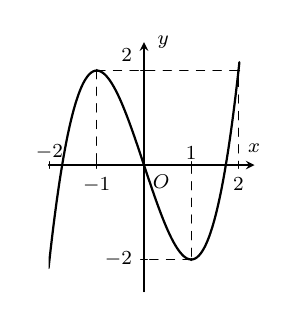
\begin{tikzpicture}[>=stealth,line join=round,line cap=round,font=\footnotesize,scale=0.6]			
			\draw[->,color=black] (-2.02,0.) -- (2.34,0.);
			\foreach \x in {-1,2}
			\draw[shift={(\x,0)},color=black] (0pt,2pt) -- (0pt,-2pt) node[below] {$\x$};
			\foreach \x in {-2,1}
			\draw[shift={(\x,0)},color=black] (0pt,2pt) -- (0pt,-2pt) node[above] {$\x$};
			\draw[color=black] (2.02,0.08) node [anchor=south west] {$x$};
			\draw[->,color=black] (0.,-2.68) -- (0.,2.6);
			\foreach \y in {-2}
			\draw[shift={(0,\y)},color=black] (2pt,0pt) -- (-2pt,0pt) node[left] {$\y$};
			\foreach \y in {2}
			\draw[shift={(0,\y)},color=black] (2pt,0pt) -- (-2pt,0pt) node[above left] {$\y$};
			\draw[color=black] (0.1,2.6) node [anchor=west] { $y$};
			\draw[color=black] (0pt,-10pt) node[right] {$\tiny  {\text{O}}$};
			\clip(-2.02,-2.68) rectangle (2.34,2.66);
			\draw[smooth][line width=0.8pt,color=black,smooth,samples=100,domain=-2.02:2.02] plot(\x,{(\x^3.0-3.0*\x});
			\draw [dashed] (-1.,2.)-- (0,2)--(2,2)--(2,0);
			\draw [dashed] (-1.,2.)-- (-1.,0.);
			\draw [dashed] (1.,0.)-- (1.,-2.);
			\draw [dashed] (1.,-2.)-- (0.,-2.);
			\fill (1,-2) circle(1pt) 
			(-1,2) circle(1pt)(2,2) circle(1pt);	
	\end{tikzpicture}}
	\loigiai{ \begin{enumerate}[a)]
			\item
			Từ đồ thị, ta có hàm số đồng biến trên các khoảng $(-\infty; -1)$ và $(1; +\infty)$, nghịch biến trên khoảng $(-1;1)$.
			\item Từ đồ thị ta thấy trên đoạn $[0;2]$ hàm số đã cho có giá trị nhỏ nhất bằng $-2$ và giá trị nhỏ nhất bằng $2$.
	\end{enumerate}}
\end{bt}

% từ: cau-hoi/lop10/0D3_Ham_so_bac_hai_va_do_thi/0D3-1-5_Tinh_dong_bien_nghich_bien.tex
\begin{bt}%[0D3H1-5]%[0K6BE-3]%[ma:997edf8f]
	Vẽ đồ thị của các hàm số $y=-x-2$ và $y=-\dfrac{1}{2}x^2$.\\
	Hãy cho biết
	\begin{enumerate}[a)]
		\item Hàm số $y=-x-2$ đồng biến hay nghịch biến trên $\mathbb{R}$?
		\item Hàm số $y=-\dfrac{1}{2}x^2$ đồng biến hay nghịch biến trên $(-\infty;\,0)$ và $(0;\,+\infty)$?
	\end{enumerate}
	\loigiai{
		\immini
		{Vẽ đồ thị $y=-x-2$}
		{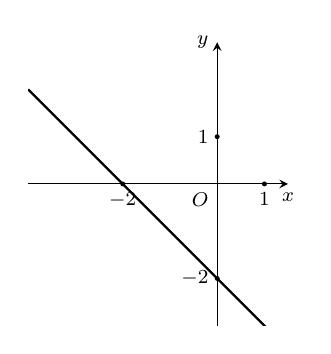
\begin{tikzpicture}[>=stealth,x=1cm,y=1cm,font=\footnotesize,scale=0.6]
				\draw[->] (-4,0) -- (1.5,0) node[below] {$x$};
				\draw[->] (0,-3) -- (0,3) node[left] {$y$};
				\draw (0,0)node[below left]{$O$};
				\fill (-2,0)node[below]{$-2$} circle(1.5pt);
				\fill (1,0)node[below]{$1$} circle(1.5pt);
				\fill (0,1)node[left]{$1$} circle(1.5pt);
				\fill (0,-2)node[left]{$-2$} circle(1.5pt);
				\clip (-4,-3)rectangle(1.5,3);
				\draw[thick,samples=150,smooth,domain=-4:1.5] plot(\x,{-\x-2});
		\end{tikzpicture}}
		\immini
		{Vẽ đồ thị $y=-\dfrac{1}{2}x^2$}
		{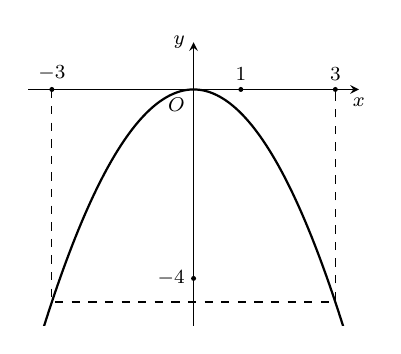
\begin{tikzpicture}[>=stealth,x=1cm,y=1cm,font=\footnotesize,scale=0.6]
				\def\a{-1/2}
				\draw[->] (-3.5,0) -- (3.5,0) node[below] {$x$};
				\draw[->] (0,-5) -- (0,1) node[left] {$y$};
				\draw (0,0)node[below left]{$O$};
				\fill (-3,0)node[above]{$-3$} circle(1.5pt);
				\fill (1,0)node[above]{$1$} circle(1.5pt);
				\fill (3,0)node[above]{$3$} circle(1.5pt);
				\fill (0,-4)node[left]{$-4$} circle(1.5pt);
				\clip (-3.5,-5)rectangle(3.5,1);
				\draw[thick,samples=150,smooth,domain=-3.5:3.5] plot(\x,{\a*(\x)^2});
				\draw[dashed] (-3,0)--(-3,-9/2)--(3,-9/2)--(3,0);
		\end{tikzpicture}}
		\begin{enumerate}[a)]
			\item Từ đồ thị của hàm số $y=-x-2$ ta thấy đồ thị của hàm số là một đường đi xuống từ trái qua phải nên hàm số đã cho là hàm nghịch biến trên $\mathbb{R}$.
			\item Từ đồ thị của hàm số $y=-\dfrac{1}{2}x^2$ ta thấy đồ thị của hàm số ở bên trái trục tung là một đường đi lên từ trái qua phải nên hàm số đã cho là hàm đồng biến trên khoảng $(-\infty;\,0)$ và đồ thị của hàm số ở bên phải trục tung là một đường đi xuống từ trái qua phải nên hàm số đã cho là hàm nghịch biến trên khoảng $(0;\,+\infty)$.
		\end{enumerate}
	}
\end{bt}

% từ: cau-hoi/lop10/0D3_Ham_so_bac_hai_va_do_thi/0D3-1-5_Tinh_dong_bien_nghich_bien.tex
\begin{bt}%[0D3H1-5]%[Dự án đề kiểm tra HKII-22-23-Nguyễn Tài Tuệ]%[ma:c8b4e9b6]
	Xét tính đồng biến, nghịch biến cùa hàm số $f(x)=\dfrac{-3}{2 x-10}$ trên khoảng $(5 ;+\infty)$.
	\loigiai{$\forall x_1 ; x_2\in(5 ;+\infty)$, giả sử $x_1<x_2\Leftrightarrow x_1-x_2<0$.\\
	Ta có 	$f\left(x_1\right)-f\left(x_2\right)=\dfrac{-3}{2x_1-10}+\dfrac 3{2x_2-10}=\dfrac{6\left(x_1-x_2\right)}{\left(2x_1-10\right)\cdot\left(2x_2-10\right)}$.\\
	Vì $x_1 ; x_2\in(5 ;+\infty)$ nên $\heva{&2x_1-10>0\\ &2x_2-10>0}$ và $x_1-x_2<0$.\\
	Do đó $f(x)_1-f\left(x_2\right)<0$.\\
	Vậy hàm số đã cho đồng biến trên khoảng $(5 ;+\infty)$.
	}
\end{bt}

% từ: cau-hoi/lop10/0D3_Ham_so_bac_hai_va_do_thi/0D3-1-5_Tinh_dong_bien_nghich_bien.tex
\begin{bt}%[0D3H1-5]%ID%[Dự án đề kiểm tra Toán 10 GHKI NH23-24- Tacgia]%[THPT ]%[ma:9dc7fab7]
	Xét tính đồng biến và nghịch biến của hàm số $f(x)=2x^2-7$ trên khoảng $(2;5)$.
	\loigiai{
		Hàm với xác định định với mọi $x\in\mathbb{R}$. Suy ra nó xác định trên khoảng $(2;5)$.\\
		Lấy $x_1,x_2$ là hai số túy ý thuộc khoảng $(2;5)$ sao cho $2<x_1<x_2<5$, ta có \[f(x_1)-f(x_2)=(2x_1^2-7)-(2x_2^2-7)=2(x_1-x_2)(x_1+x_2).\]
		Do $2<x_1<x_2<5$ nên $x_1-x_2<0$. Suy ra $f(x_1)-f(x_2)<0$ hay $f(x_1)<f(x_2)$.\\
		Vậy hàm số đã cho đồng biến trên khoảng $(2;5)$.
	}
\end{bt}

% từ: cau-hoi/lop10/0D3_Ham_so_bac_hai_va_do_thi/0D3-1-5_Tinh_dong_bien_nghich_bien.tex
\begin{bt}%[0D3H1-5]%[Đề thi HK1, THPT Ten lơ Man-TPHCM-TuanBC]%[ma:86e927fb]
	Xét sự đồng biến, nghịch biến của hàm số $y=f(x)=3x^2$ trên khoảng $(-\infty;0)$.
	\loigiai{
Ta có bảng biến thiên của hàm số như sau:
\begin{center}
	
\begin{tikzpicture}
		\tkzTabInit[lgt=1.2,espcl=4]
		{$x$/1.2,$y$/2.5}
		{$-\infty$,$0$,$+\infty$}
		\tkzTabVar{+/$+\infty$,-/$0$,+/$+\infty$}
	\end{tikzpicture}
\end{center}	
Hàm số nghịch biến trên khoảng $(-\infty;0)$.
}
\end{bt}

% từ: cau-hoi/lop10/0D3_Ham_so_bac_hai_va_do_thi/0D3-1-5_Tinh_dong_bien_nghich_bien.tex
\begin{bt}%[0D3H1-5]%[ma:3c5f651b]
	Cho hàm số $y=f(x)$ có đồ thị như hình vẽ bên dưới. Hãy chỉ ra những khoảng đồng biến và nghịch biến của hàm số $y=f(x)$.
	\begin{center}
		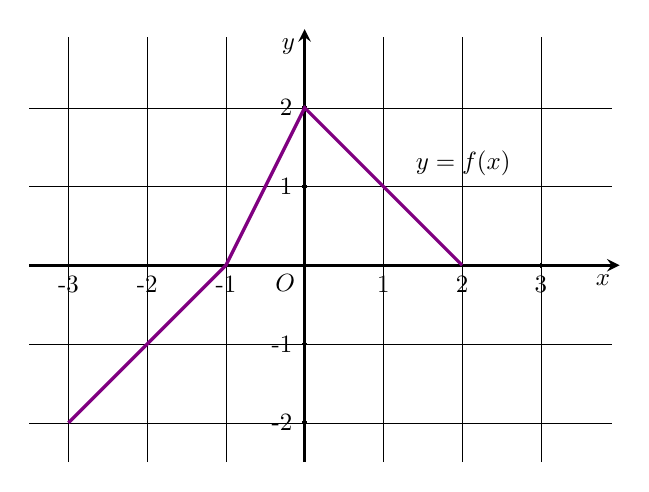
\begin{tikzpicture}[>=stealth,x=1cm,y=1cm]
		\draw[line width=0.1pt] (-3.5,-2.5) grid (3.9,2.9);
		\draw[->,line width=1pt](-3.5,0)--(0,0)node[below left]{$O$}--(4,0)node[below left]{$x$};
		\draw[->,line width=1pt](0,-2.5)--(0,3)node[below left]{$y$};
		\foreach \x in {-3,-2,-1,1,2,3}
		\draw[thin] (\x,1pt)--(\x,-1pt) node[below]{\x};
		\foreach \y in {-2,-1,1,2}
		\draw[line width=1pt] (1pt,\y)--(-1pt,\y) node[left]{\y};
		\draw[-,violet, line width=1.2pt] (-3,-2)--(-1,0)--(0,2)--(2,0);
		\node at (1.3,1.3)[right]{$y=f(x)$};
		\end{tikzpicture}
	\end{center}
	\loigiai{
		Hàm số đồng biến trên khoảng $(-3;0)$. \\
		Hàm só nghịch biến trên khoảng $(0;2)$.
	}
\end{bt}

% từ: cau-hoi/lop10/0D3_Ham_so_bac_hai_va_do_thi/0D3-2-1_Xac_dinh_ham_so_bac_hai.tex
\begin{ex}%[0D3B2-1]%[ma:d49aec93]
	Tung một đồng xu cân đối và đồng chất hai lần liên tiếp. Tính xác suất để cả hai lần tung đều xuất hiện  mặt ngửa.
	 \choice
		 {$\dfrac{1}{3}$}
		 {$\dfrac{1}{2}$}
		 {$\dfrac{3}{4}$}
		 {\True $\dfrac{1}{4}$}
	 \loigiai{
		Số phần tử  của không gian mẫu $ n(\Omega)=4 $.\\
		Biế cố hai lần đều xuất hiện mặt ngửa $  A=\{NN\} \Rightarrow n\left(A\right) =1$.\\
		 Do đó xác suất cần tìm là $ P(A)=\dfrac{1}{4} $.
	 }
\end{ex}

% từ: cau-hoi/lop10/0D3_Ham_so_bac_hai_va_do_thi/0D3-2-2_Bang_bien_thien_tinh_don_dieu_max_min.tex
\begin{bt}%[0D3H2-2]%[ma:687e2956]
	Tìm giá trị lớn nhất của hàm số $y=-2x^2+x+5$. Kết quả  làm tròn đến hàng phần mười.
	 \shortans{0,3}
	 \loigiai{
		Xét  hàm số $y=-2x^2+x+5$ có $a=-2< 0$ và có đỉnh $I\left(\dfrac{1}{4}; \dfrac{41}{8}\right)$.\\
		Do đó,  hàm số đạt giá trị lớn nhất bằng $\dfrac{41}{8}$ tại $x=\dfrac{1}{4}\approx0{,}3$.
	} 
\end{bt}

% từ: cau-hoi/lop10/0D3_Ham_so_bac_hai_va_do_thi/0D3-2-3_Do_thi_cua_ham_so_bac_hai.tex
\begin{ex}%[0D3H2-3]%[ma:06c1e007]
	Hàm số $y=ax^2+bx+c$ với $a>0$; $ b>0$ và $c<0$ có đồ thị là đường  cong nào dưới đây?
	 \choice
		{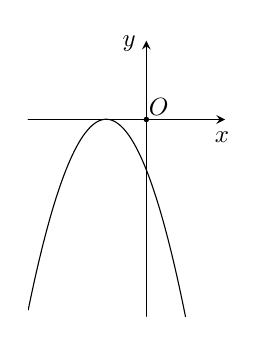
\begin{tikzpicture}[font=\footnotesize,line join=round,line cap=round,>=stealth]
		\tikzset{declare function={xmin=-1.5; xmax=1; ymin=-2.5; ymax=1; 
			f (\x)=-2.47*(\x)^2-2.52*(\x)-0.64; 
			 },
			 smooth,samples=450
		} 
		\draw[->] (xmin,0)--(xmax,0) node[shift={(-100:7pt)},font=\normalsize]{$ x  $};
		 \draw[->] (0,ymin)--(0,ymax) node[shift={(190:7pt)},font=\normalsize]{$ y $};
		\fill  (0,0) node[shift={(45:7pt)},font=\normalsize]{$ O $};
		\fill (0,0) circle  (1pt);
		\clip (xmin,ymin) rectangle (xmax,ymax); 
		\draw plot[domain=xmin:xmax] (\x,{f  (\x)});
	\end{tikzpicture}
		} 
		{\begin{tikzpicture}[font=\footnotesize,line join=round,line cap=round,>=stealth]
		\tikzset{declare function={xmin=-1.5; xmax=2.5; ymin=-1;  ymax=2.5;
			f (\x)=-1.3*(\x)^2+1.3*(\x)+1.6; 
			 },
			smooth,samples=450 
		 }
		\draw[->] (xmin,0)--(xmax,0) node[shift={(-100:7pt)},font=\normalsize]{$  x $};
		\draw[->] (0,ymin)--(0,ymax) node[shift={(190:7pt)},font=\normalsize]{$ y $}; 
		\fill (0,0) node[shift={(45:7pt)},font=\normalsize]{$ O  $};
		\fill (0,0) circle  (1pt);
		\clip (xmin,ymin) rectangle (xmax,ymax); 
		\draw  plot[domain=xmin:xmax] (\x,{f (\x)});
	\end{tikzpicture}
		 }
		{\True 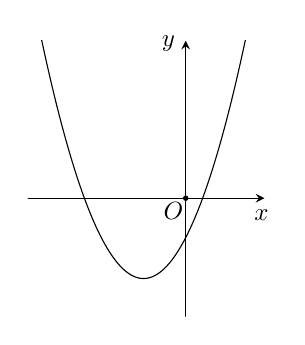
\begin{tikzpicture}[font=\footnotesize,line join=round,line cap=round,>=stealth]
		\tikzset{declare function={xmin=-2; xmax=1; ymin=-1.5;  ymax=2;
			f (\x)=1.81*(\x)^2+1.94*(\x)-0.5; 
			}, 
			smooth,samples=450 
		} 
		\draw[->] (xmin,0)--(xmax,0)  node[shift={(-100:7pt)},font=\normalsize]{$ x $};
		\draw[->] (0,ymin)--(0,ymax) node[shift={(190:7pt)},font=\normalsize]{$ y $}; 
		\fill (0,0)  node[shift={(-135:7pt)},font=\normalsize]{$ O $};
		 \fill (0,0) circle (1pt);
		 \clip (xmin,ymin) rectangle (xmax,ymax);
		\draw plot[domain=xmin:xmax]  (\x,{f (\x)});
	\end{tikzpicture}
		 }
		{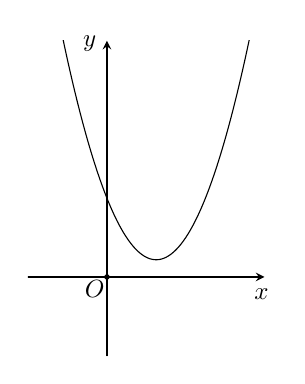
\begin{tikzpicture}[font=\footnotesize,line join=round,line cap=round,>=stealth]
		\tikzset{declare function={xmin=-1; xmax=2; ymin=-1; ymax=3; 
			f (\x)=2*(\x)^2-2.5*(\x)+1; 
			}, 
			smooth,samples=450 
		} 
		\draw[->]  (xmin,0)--(xmax,0) node[shift={(-100:7pt)},font=\normalsize]{$ x $};
		\draw[->] (0,ymin)--(0,ymax) node[shift={(190:7pt)},font=\normalsize]{$  y $};
		 \fill (0,0) node[shift={(-135:7pt)},font=\normalsize]{$ O $};
		\fill (0,0) circle  (1pt);
		\clip (xmin,ymin) rectangle (xmax,ymax); 
		\draw  plot[domain=xmin:xmax] (\x,{f (\x)});
	\end{tikzpicture}
		 }
	 \loigiai{
		Đồ thị hàm số $a>0$ nên bề  lõm đồ thị quay lên và $c<0$ nên đồ thị cắt trục $Oy$ tại điểm có tung độ âm.
		\begin{center}
			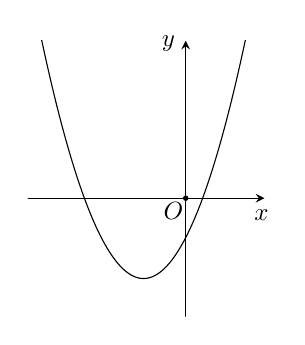
\begin{tikzpicture}[font=\footnotesize,line join=round,line cap=round,>=stealth]
					\tikzset{declare  function={xmin=-2; xmax=1; ymin=-1.5; ymax=2;
						f  (\x)=1.81*(\x)^2+1.94*(\x)-0.5;
						}, 
						smooth,samples=450 
					} 
					 \draw[->] (xmin,0)--(xmax,0) node[shift={(-100:7pt)},font=\normalsize]{$ x $};
					 \draw[->] (0,ymin)--(0,ymax) node[shift={(190:7pt)},font=\normalsize]{$ y $};
					\fill (0,0)  node[shift={(-135:7pt)},font=\normalsize]{$ O $};
					\fill (0,0) circle  (1pt);
					 \clip (xmin,ymin) rectangle (xmax,ymax);
					 \draw plot[domain=xmin:xmax] (\x,{f (\x)});
				\end{tikzpicture}
		\end{center}
	} 
\end{ex}

% từ: cau-hoi/lop10/0D3_Ham_so_bac_hai_va_do_thi/0D3-2-3_Do_thi_cua_ham_so_bac_hai.tex
\begin{ex}%[0D3K2-3]%[ma:6c57620d]
	 Đồ thị dưới đây là của hàm số nào?
	\begin{center}
		\begin{tikzpicture}[scale=0.85,>=stealth,font=\footnotesize,line join=round,line cap=round]
				\def\xmin{-2}  \def\xmax{5}
				 \def\ymin{-2} \def\ymax{6}
				\draw[->] (\xmin,0)--(\xmax,0)  node [below]{$x$};
				\draw[->] (0,\ymin)--(0,\ymax) node [left]{$y$}; 
				\node at (0,0) [below left]{$O$}; 
				\clip (\xmin+0.1,\ymin+0.1)  rectangle (\xmax-0.5,\ymax-0.1);
				\draw[smooth,samples=300,domain=-1.5:4.5] plot  (\x,{(\x)^2-4*(\x)+3});
				\draw[dashed] (2,-2)--(2,5) 
					 (0,-1)--(2,-1);
				\draw (-1,0) node[below]  {$-1$}
					 (1,0) node[below left] {$1$}
					(2,0) node  [below right] {$2$}
					(3,0) node[below  right] {$3$}
					(4,0) node[below]  {$4$};
				 \draw (0,-1) node[left] {$-1$}
					(0,1) node[left]  {$1$}
					(0,2) node  [left] {$2$}
					(0,3) node[left] {$3$} 
					 (0,4) node[right] {$4$};
			\end{tikzpicture}
	\end{center}
	\choice 
		{$y=x^2-4x-1$} 
		 {\True $y=x^2-4x+3$}
		 {$y=-x^2+4x-1$}
		 {$y=-x^2+4x+3$}
	 \loigiai{
		Parabol  có bề lõm hướng lên trên nên $a>0$, hơn nữa parabol cắt $Oy$ tại điểm $(0;3)$ nên $c=3$. Do đó đồ thị trong hình vẽ là đồ thị của hàm số $y=x^2-4x+3$.
	} 
\end{ex}

% từ: cau-hoi/lop10/0D3_Ham_so_bac_hai_va_do_thi/0D3-2-3_Do_thi_cua_ham_so_bac_hai.tex
\begin{bt}%[0D3N2-3]%[6.7 sách kết nối]%[ma:ebdd503c]
	Vẽ các đường parabol sau
	\begin{multicols}{2}
		\begin{enumerate}
			\item $y=x^2-3x+2$
			\item $y=-2x^2+2x+3$
			\item $y=x^2+2x+1$
			\item $y=-x^2+x-1$
		\end{enumerate}
	\end{multicols}
	\loigiai{
		\begin{enumerate}		
			\item \immini{Tập xác định $\mathscr{D}=\mathbb{R}$.\\
			Đỉnh $I\left(\dfrac{3}{2}\,;\,-\dfrac{1}{4}\right)$.\\
			Trục đối xứng  $x=\dfrac{3}{2}$.\\
			Đồ thị của hàm số cắt trục $Ox$ tại hai điểm
			$A\left(1\,;\,0\right), B\left(2\,;\,0\right)$ và cắt trục $Oy$ tại một điểm $C\left(0\,;\,2\right)$.\\
			Ta có đồ thị $\left(P\right)$ như hình vẽ.}
			{
				\begin{tikzpicture}[>=latex, scale=1,font=\footnotesize]
					\draw[->,line width =1pt] (-2,0)--(0,0)node [above left]{$ O $}--(4,0) node[above]{$x$};
					\draw[->,line width =1pt] (0,-1)--(0,3) node[right]{$y$};
					\fill (0,0) circle (1.5pt);
					\draw[ smooth, line width=1pt,samples=100] plot[domain=-0.2:3.2] (\x,{(\x)^2-3*\x+2});
					\fill (1.5,0) node[above]{$\dfrac{3}{2}$} circle (1.5pt);
					\fill (1,0) node[above]{$1$} circle (1.5pt);
					\fill (2,0) node[above]{$2$} circle (1.5pt);
					\fill (3,0) node[below]{$3$} circle (1.5pt);
					\fill (0,-0.25) node[below left]{$-\dfrac{1}{4}$} circle (1.5pt);
					\fill (0,2) node[left]{$2$} circle (1.5pt);
					\draw[dashed,line width=1pt] (0,2)--(3,2)--(3,0) ;
					\draw[dashed,line width=1pt] (0,-0.25)--(1.5,-0.25)--(1.5,0) ;
					\fill (1.5,-0.25) circle (1.5pt);
				\end{tikzpicture}
			}
			\item \immini{Tập xác định $\mathscr{D}=\mathbb{R}$.\\
			Đỉnh $I\left(\dfrac{1}{2}\,;\,\dfrac{7}{2}\right)$.\\
			Trục đối xứng  $x=\dfrac{1}{2}$.\\
			Đồ thị của hàm số cắt trục $Ox$ tại hai điểm
			$A\left(\dfrac{1+\sqrt{7}}{2}\,;\,0\right), B\left(\dfrac{1-\sqrt{7}}{2}\,;\,0\right)$ và cắt trục $Oy$ tại một điểm $C\left(0\,;\,3\right)$.\\
			Ta có đồ thị $\left(P\right)$ như hình vẽ.}{
				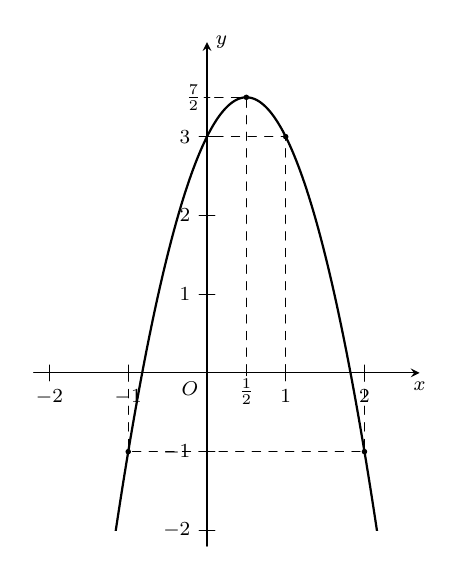
\begin{tikzpicture}[scale=1, font=\footnotesize, line join=round, line cap=round, >=stealth]
					\def\xmin{-2}\def\xmax{2.5}\def\ymin{-2}\def\ymax{4}
					\draw[->] (\xmin-0.2,0)--(\xmax+0.2,0) node[below] {\footnotesize $x$};
					\draw[->] (0,\ymin-0.2)--(0,\ymax+0.2) node[right] {\footnotesize $y$};
					\draw (0,0) node [below left] {\footnotesize $O$};
					\foreach \x in {-2,-1,1,2}\draw (\x,0.1)--(\x,-0.1) node [below] {\footnotesize $\x$};
					\foreach \y in {-2,-1,1,2,3}\draw (0.1,\y)--(-0.1,\y) node [left] {\footnotesize $\y$};
					\clip (\xmin,\ymin) rectangle (\xmax,\ymax);
					\draw[thick,smooth,samples=200,domain=\xmin:\xmax] plot (\x,{-2*((\x)^2)+2*\x+3});
					\draw[dashed] (0.5,0)--(0.5,3.5)--(0,3.5);\fill (0.5,3.5) circle (1pt);
					\draw (0.5,-1pt)--(0.5,1pt) node [below] {\footnotesize $\frac{1}{2}$};
					\draw (-1pt,3.5)--(1pt,3.5) node [left] {\footnotesize $\frac{7}{2}$};
					\draw[dashed] (-1,0)--(-1,-1)--(0,-1);\fill (-1,-1) circle (1pt);
					\draw[dashed] (1,0)--(1,3)--(0,3);\fill (1,3) circle (1pt);
					\draw[dashed] (2,0)--(2,-1)--(0,-1);\fill (2,-1) circle (1pt);
				\end{tikzpicture}
			}
			\item \immini{Tập xác định $\mathscr{D}=\mathbb{R}$.\\
			Đỉnh $I\left(-1\,;\,0\right)$.\\
			Trục đối xứng  $x=-1$.\\
			Đồ thị của hàm số cắt trục $Ox$ tại một điểm
			$A\left(-1\,;\,0\right)$ và cắt trục $Oy$ tại một điểm $C\left(0\,;\,1\right)$.\\
			Ta có đồ thị $\left(P\right)$ như hình vẽ.}{
				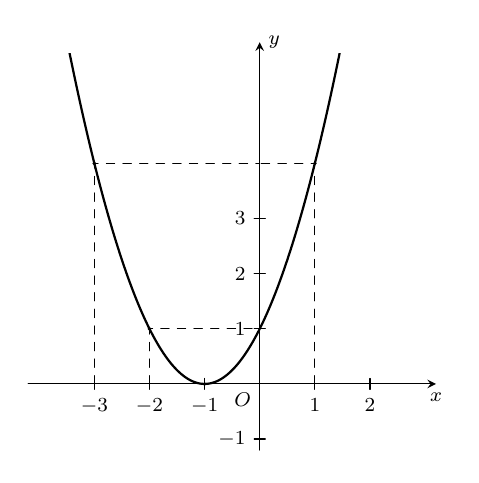
\begin{tikzpicture}[scale=0.7, font=\footnotesize, line join=round, line cap=round, >=stealth]
					\def\xmin{-4}\def\xmax{3}\def\ymin{-1}\def\ymax{6}
					\draw[->] (\xmin-0.2,0)--(\xmax+0.2,0) node[below] {\footnotesize $x$};
					\draw[->] (0,\ymin-0.2)--(0,\ymax+0.2) node[right] {\footnotesize $y$};
					\draw (0,0) node [below left] {\footnotesize $O$};
					\foreach \x in {-3,-2,-1,1,2}\draw (\x,0.1)--(\x,-0.1) node [below] {\footnotesize $\x$};
					\foreach \y in {-1,1,2,3}\draw (0.1,\y)--(-0.1,\y) node [left] {\footnotesize $\y$};
					\clip (\xmin,\ymin) rectangle (\xmax,\ymax);
					\draw[thick,smooth,samples=200,domain=\xmin:\xmax] plot (\x,{1*((\x)^2)+2*\x+1});
					\draw[dashed] (-1,0)--(-1,0)--(0,0);\fill (-1,0) circle (1pt);
					\draw[dashed] (-3,0)--(-3,4)--(0,4);\fill (-3,4) circle (1pt);
					\draw[dashed] (-2,0)--(-2,1)--(0,1);\fill (-2,1) circle (1pt);
					\draw[dashed] (1,0)--(1,4)--(0,4);\fill (1,4) circle (1pt);
				\end{tikzpicture}
			}
			\item \immini{Tập xác định $\mathscr{D}=\mathbb{R}$.\\
			Đỉnh $I\left(\dfrac{1}{2}\,;\,-\dfrac{3}{4}\right)$.\\
			Trục đối xứng  $x=\dfrac{1}{2}$.\\
			Ta có đồ thị $\left(P\right)$ như hình vẽ.}{
				\begin{tikzpicture}[scale=1, font=\footnotesize, line join=round, line cap=round, >=stealth]
					\def\xmin{-2}\def\xmax{3}\def\ymin{-4}\def\ymax{1}
					\draw[->] (\xmin-0.2,0)--(\xmax+0.2,0) node[below] {\footnotesize $x$};
					\draw[->] (0,\ymin-0.2)--(0,\ymax+0.2) node[right] {\footnotesize $y$};
					\draw (0,0) node [above left] {\footnotesize $O$};
					\foreach \x in {-1,1,2}\draw (\x,0.1)--(\x,-0.1) node [below] {\footnotesize $\x$};
					\foreach \y in {-3,-2,-1,1}\draw (0.1,\y)--(-0.1,\y) node [left] {\footnotesize $\y$};
					\clip (\xmin,\ymin) rectangle (\xmax,\ymax);
					\draw[thick,smooth,samples=200,domain=\xmin:\xmax] plot (\x,{-1*((\x)^2)+1*\x+-1});
					\draw[dashed] (0.5,0)--(0.5,-0.75)--(0,-0.75);\fill (0.5,-0.75) circle (1pt);
					\draw (0.5,1pt)--(0.5,-1pt) node [above] {\footnotesize $\frac{1}{2}$};
					\draw (-1pt,-0.75)--(1pt,-0.75) node [left] {\footnotesize $-\frac{3}{4}$};
					\draw[dashed] (-1,0)--(-1,-3)--(0,-3);\fill (-1,-3) circle (1pt);
					\draw[dashed] (1,0)--(1,-1)--(0,-1);\fill (1,-1) circle (1pt);
					\draw[dashed] (2,0)--(2,-3)--(0,-3);\fill (2,-3) circle (1pt);
				\end{tikzpicture}
			}
		\end{enumerate}
	}
\end{bt}

% từ: cau-hoi/lop10/0D7_Bat_phuong_trinh_bac_2_mot_an/0D7-2-2_Giai_bat_phuong_trinh_bac_hai_biet_BXD_do_thi.tex
\begin{bt}%[0D7H2-2]%[Tex hóa SGK CD-CT,T7/22, Tuấn Nguyễn]%Bài 4%[ma:67c2f5fd]
	Dựa vào đồ thị của hàm số bậc hai được cho, hãy giải các bất phương trình sau
	\begin{listEX}[2]
		\item $f(x) \geq 0$.
		\begin{center}
			\begin{tikzpicture}[scale=1,font=\footnotesize,line cap=round,line join=round,>=stealth]
				\def\a{-1/2} \def\b{5.5/2} \def\c{-6/2} % Hệ số
				\def\xt{-1} \def\xp{5} \def\yt{1} \def\yd{-2} % x_trái, x_phải, y_trên, y_dưới (giới hạn)
				\draw[->] (\xt,0)--(\xp,0) node [below]{$x$};
				\draw[->] (0,\yd)--(0,\yt) node [left]{$y$};
				\node at (0,0) [below left]{$O$};
				\clip (\xt-0.1,\yd+0.1) rectangle (\xp-0.1,\yt-0.1);
				\draw[smooth,samples=300] plot(\x,{\a*(\x)^2+\b*(\x)+\c});
				\draw[fill=black] (1.5,0) node[shift={(-90:.4)}]{$\tfrac{3}{2}$} circle(1pt);\draw[fill=black] (4,0) node[shift={(-90:.4)}]{$4$} circle(1pt);
				\draw (1,-1) node[shift={(0:.6)}]{$y=f(x)$};
			\end{tikzpicture}
		\end{center}
		\item $f(x)>0$.
		\begin{center}
			\begin{tikzpicture}[scale=.6,font=\footnotesize,line cap=round,line join=round,>=stealth]
				\def\a{1/2} \def\b{-2/2} \def\c{-3/2} % Hệ số
				\def\xt{-2} \def\xp{4} \def\yt{2} \def\yd{-3} % x_trái, x_phải, y_trên, y_dưới (giới hạn)
				\draw[->] (\xt,0)--(\xp,0) node [below]{$x$};
				\draw[->] (0,\yd)--(0,\yt) node [left]{$y$};
				\node at (0,0) [above right]{$O$};
				%\clip (\xt-0.1,\yd+0.1) rectangle (\xp-0.1,\yt-0.1);
				\draw[smooth,samples=300,domain=-1.5:3.5] plot(\x,{\a*(\x)^2+\b*(\x)+\c});
				\draw[fill=black] (-1,0) node[shift={(-145:.4)}]{$-1$} circle(1pt);\draw[fill=black] (3,0) node[shift={(-70:.4)}]{$3$} circle(1pt);
				\draw (4,1) node[shift={(0:.4)}]{$y=f(x)$};
			\end{tikzpicture}
		\end{center}
		\item $f(x) \leq 0$.
		\begin{center}
			\begin{tikzpicture}[scale=1,font=\footnotesize,line cap=round,line join=round,>=stealth]
				\def\a{1} \def\b{-2} \def\c{1} % Hệ số
				\def\xt{-1} \def\xp{3} \def\yt{4} \def\yd{-1} % x_trái, x_phải, y_trên, y_dưới (giới hạn)
				\draw[->] (\xt,0)--(\xp,0) node [below]{$x$};
				\draw[->] (0,\yd)--(0,\yt) node [left]{$y$};
				\node at (0,0) [below left]{$O$};
				\clip (\xt-0.1,\yd+0.1) rectangle (\xp-0.1,\yt-0.1);
				\draw[smooth,samples=300,domain=-3.5:5.8] plot(\x,{\a*(\x)^2+\b*(\x)+\c});
				\draw[fill=black] (1,0) node[shift={(-90:.4)}]{$1$} circle(1pt);
				\draw (2,3) node[shift={(180:.1)}]{$y=f(x)$};
			\end{tikzpicture}
		\end{center}
		\item $f(x)<0$.
		\begin{center}
			\begin{tikzpicture}[scale=1,font=\footnotesize,line cap=round,line join=round,>=stealth]
				\def\a{1} \def\b{2} \def\c{1.5} % Hệ số
				\def\xt{-3} \def\xp{1} \def\yt{3} \def\yd{-1} % x_trái, x_phải, y_trên, y_dưới (giới hạn)
				\draw[->] (\xt,0)--(\xp,0) node [below]{$x$};
				\draw[->] (0,\yd)--(0,\yt) node [left]{$y$};
				\node at (0,0) [below left]{$O$};
				\clip (\xt-0.1,\yd+0.1) rectangle (\xp-0.1,\yt-0.1);
				\draw[smooth,samples=300,domain=-3:1] plot(\x,{\a*(\x)^2+\b*(\x)+\c});
				\draw (-2.5,2.5) node[shift={(0:1)}]{$y=f(x)$};
			\end{tikzpicture}	
		\end{center}
		\item $f(x)<0$.
		\begin{center}
			\begin{tikzpicture}[scale=1,font=\footnotesize,line cap=round,line join=round,>=stealth]
				\def\a{-1/3} \def\b{6/3} \def\c{-9/3} % Hệ số
				\def\xt{-1} \def\xp{6} \def\yt{1} \def\yd{-3} % x_trái, x_phải, y_trên, y_dưới (giới hạn)
				\draw[->] (\xt,0)--(\xp,0) node [below]{$x$};
				\draw[->] (0,\yd)--(0,\yt) node [left]{$y$};
				\node at (0,0) [below left]{$O$};
				\clip (\xt-0.1,\yd+0.1) rectangle (\xp-0.1,\yt-0.1);
				\draw[smooth,samples=300,domain=-0.1:5.8] plot(\x,{\a*(\x)^2+\b*(\x)+\c});
				\draw[fill=black] (3,0) node[shift={(-90:.4)}]{$3$} circle(1pt);
				\draw (1,-2) node[shift={(0:.4)}]{$y=f(x)$};
			\end{tikzpicture}
		\end{center}
		\item $f(x) \leq 0$.
		\begin{center}
			\begin{tikzpicture}[scale=1,font=\footnotesize,line cap=round,line join=round,>=stealth]
				\def\a{-1} \def\b{-2} \def\c{-1.5} % Hệ số
				\def\xt{-3} \def\xp{1} \def\yt{1} \def\yd{-3} % x_trái, x_phải, y_trên, y_dưới (giới hạn)
				\draw[->] (\xt,0)--(\xp,0) node [below]{$x$};
				\draw[->] (0,\yd)--(0,\yt) node [left]{$y$};
				\node at (0,0) [below left]{$O$};
				\clip (\xt-0.1,\yd+0.1) rectangle (\xp-0.1,\yt-0.1);
				\draw[smooth,samples=300,domain=-3.5:5.8] plot(\x,{\a*(\x)^2+\b*(\x)+\c});
				\draw (-2.5,-2.5) node[shift={(0:1)}]{$y=f(x)$};
			\end{tikzpicture}
		\end{center}
	\end{listEX}
	\loigiai{
		\begin{listEX}[3]
			\item $\dfrac{3}{2} \leq x \leq 4$.
			\item $x<-1$ hoặc $x>3$.
			\item $x=1$.
			\item Vô nghiệm.
			\item $x \ne 3$.
			\item $x \in \mathbb{R}$.
		\end{listEX}
	}
\end{bt}

% từ: cau-hoi/lop10/0D7_Bat_phuong_trinh_bac_2_mot_an/0D7-2-6_Bai_toan_co_tham_so.tex
\begin{bt}%[Bài Giảng K10-K11, Đỗ Viết Lân]%[0D7V2-6]%[ma:ef63ded4]
	Tìm các giá trị của tham số $m$ để tam thức bậc hai $x^2+(m-1)x+2m+7\geq 0 ,\,\forall x \in \mathbb{R}.$
	\loigiai{
		\allowdisplaybreaks
		\begin{eqnarray*}
			x^2+(m-1)x+2m+7\geq 0,\,\forall x \in \mathbb{R}&\Leftrightarrow& \heva{& 1>0\\& (m+1)^2-4\cdot 1\cdot (2m+7)\leq 0}\\
			&\Leftrightarrow& m^2-6m-3\leq 0\\
			&\Leftrightarrow & 3-2\sqrt{3} \leq m \leq 3+2\sqrt{3}.
		\end{eqnarray*}
	}
\end{bt}

% từ: cau-hoi/lop10/0D7_Bat_phuong_trinh_bac_2_mot_an/0D7-2-6_Bai_toan_co_tham_so.tex
\begin{bt}%[Bài Giảng K10-K11, Đỗ Viết Lân]%[0D7V2-6]%[ma:8367168e]
	Tìm các giá trị của tham số $m$ để tam thức bậc hai 
	$$-2x^2+(m+2)x+m-4\leq 0,\,\forall x \in \mathbb{R}.$$	
	\loigiai{
		\allowdisplaybreaks
		\begin{eqnarray*}
			-2x^2+(m+2)x+m-4\leq 0,\,\forall x \in \mathbb{R}&\Leftrightarrow& \heva{& -2<0\\& (m+2)^2-4\cdot (-2)\cdot (m-4)\leq 0}\\
			&\Leftrightarrow& m^2 + 12m -28 \leq 0\\
			&\Leftrightarrow & -14\leq m \leq 2.
		\end{eqnarray*}
	}
\end{bt}

% từ: cau-hoi/lop10/0D7_Bat_phuong_trinh_bac_2_mot_an/0D7-3-1_Phuong_trinh_can.tex
\begin{ex}%[0D7H3-1]%[ma:a507c802]
	Cho phương trình $\sqrt{x^2-4x-2}=\sqrt{3x^2-8}$. 
	\choiceTF 
		{Phương trình  có hai nghiệm phân biệt}
		{\True Phương trình có một  nghiệm}
		 {Phương trình có nghiệm $x=1$}
		{\True Phương  trình có nghiệm $x=-3$}
	\loigiai{ 
		 Bình phương hai vế của phương trình $\sqrt{x^2-4x-2}=\sqrt{3x^2-8}$ ta được
		\begin{eqnarray*}
			 && x^2-4x-2=3x^2-8\\
			&\Leftrightarrow& -2x^2-4x+6=0\\ 
			&\Leftrightarrow&  \hoac{&x=1\\&x=-3.}
		\end{eqnarray*}
		Thay lần lượt các giá  trị của $x$ vào phương trình ta thấy chỉ có $x=-3$ thỏa mãn.\\
		Vậy phương trình có một nghiệm là $x=-3$. 
	} 
\end{ex}

% từ: cau-hoi/lop10/0D7_Bat_phuong_trinh_bac_2_mot_an/0D7-3-5_Phuong_trinh_khac_quy_ve_phuong_trinh_bac_2.tex
\begin{bt}%[0D7H3-5]%[ma:ef07da7f]
	Có tất cả bao nhiêu giá trị nguyên của tham số $m$ để phương trình $mx^2-2(m-1)x+m-3=0$ có  nghiệm duy nhất? \shortans{2}
	\loigiai{ 
		\begin{itemize}
			\item Nếu  $m=0$ thì bất phương trình đã cho trở thành
			\[2x-3=0\Leftrightarrow  x =\dfrac{3}{2}.\]
			Do đó $m=0$, phương trình đã cho có nghiệm duy nhất $x= \dfrac{3}{2}$. 
			 \item Nếu $m \neq 0$ thì $mx^2-2(m-1)x+m-3=0$ là phương trình bậc hai. Phương trình này có nghiệm duy nhất khi
			\[\Delta' =0\Leftrightarrow (m-1)^2-m(m-3)=0\Leftrightarrow m+1=0\Leftrightarrow m=-1 \  \text{(nhận)}.\]
		\end{itemize}
		Vậy với  $m=0$, $m=-1$ thì phương trình đã cho có nghiệm duy nhất.
	} 
\end{bt}

% từ: cau-hoi/lop10/0D7_Bat_phuong_trinh_bac_2_mot_an/0D7-3-6_Toan_hinh_toan_thuc_te_ung_dung_phuong_trinh.tex
\begin{bt}%[0D7H3-6]%[Tex hóa SGK CD-CT,T7/22, Tuấn Nguyễn]%[ma:f6d47162]
	\immini
	{Một ngọn hải đăng đặt tại vị trí $A$ cách bờ biển một khoảng cách $A B=4$ km. Trên bờ biển có một cái kho ở vị trí $C$ cách $B$ một khoảng là $7$ km. Người canh hải đăng có thể chèo thuyền từ $A$ đến vị trí $M$ trên bờ biển vối vận tốc $3$ km/h rồi đi bộ đến $C$ với vận tốc $5$ km/h như Hình 35 . Tính khoảng cách từ vị trí $B$ đến $M$, biết thời gian người đó đi từ $A$ đến $C$ là 148 phút.}
	{\begin{tikzpicture}[scale=0.7, font=\footnotesize, line join=round, line cap=round, >=stealth]
			\path 
			(0,4) coordinate (A)
			(0,0) coordinate (B)
			(7,0) coordinate (C)
			(3,0) coordinate (M)
			(3.5,-1) coordinate (TT) node [below]{Hình 35}
			;
			\draw (B)--(A)node[left,midway]{$4$ km}--(M);
			\draw[shorten <= -0.5cm,shorten >= -0.5cm] (B)--(C);
			\draw[dashed] (B)--+(0,-0.5)(C)--+(0,-0.5);
			\draw[<->,dashed,yshift=-0.3cm] (0,0)--(7,0) node[below,midway]{$7$ km};
			\foreach \p/\g in {A/90,B/135,C/90,M/45}\fill[black] (\p) circle (1pt) +(\g:.5)node{$\p$};
	\end{tikzpicture}}
	\loigiai{
		Gọi $BM=a$ km suy ra $MC=7-a$ km ($0<a<7$).\\
		Theo giả thiết ta có $AM=\sqrt{AB^2+BM^2}=\sqrt{4^2+a^2}$.\\
		Từ đó suy ra \begin{eqnarray*}
			&&\dfrac{\sqrt{4^2+a^2}}{3}+\dfrac{7-a}{5}=\dfrac{148}{60}=\dfrac{37}{15}\\
			&\Leftrightarrow & 5\sqrt{4^2+a^2}=3a+16\\
			&\Leftrightarrow & 25(16+a^2)=9a^2+96a+256\\
			&\Leftrightarrow & 16a^2-96a+144=0\\
			&\Leftrightarrow & a=3.
		\end{eqnarray*}
		Vậy $BM=3$ km.	
	} 
\end{bt}

% từ: cau-hoi/lop10/0D8_Dai_so_to_hop/0D8-2-6_Bai_toan_co_yeu_to_hinh_hoc.tex
\begin{ex}%[0D8N2-6]%[ma:42cbd57e]
	Cho lục giác $ABCDEF$. Chọn khẳng định đúng trong các khẳng  định sau.
	\choiceTF 
		{\True Số véc-tơ khác $\overrightarrow{0}$ có điểm đầu, điểm cuối là hai  trong $6$ đỉnh của lục giác là $30$}
		{Số véc-tơ khác  $\overrightarrow{0}$ có điểm đầu, điểm cuối là hai trong $6$ đỉnh của lục giác là $15$}
		{\True Số tam  giác tạo thành từ $6$ đỉnh của lục giác là $20$}
		{Số tam giác tạo thành từ $6$ đỉnh của  lục giác là $120$}
	 \loigiai{
		\begin{itemize}
			\item Số véc-tơ khác $\overrightarrow{0}$ có điểm đầu, điểm cuối là hai trong $6$ đỉnh của  lục giác là $\mathrm{A}_6^2=30$.
			\item Số tam giác tạo thành từ  $6$ đỉnh của lục giác là $\mathrm{C}_6^3=20$.
		\end{itemize}
	} 
\end{ex}

% từ: cau-hoi/lop10/0D8_Dai_so_to_hop/0D8-3-2_Khai_trien_mot_nhi_thuc_Newton.tex
\begin{bt}%[0D8H3-2] % KIEM_TRA%[Dự án đề kiểm tra HKII NH22-23- Nguyễn Tú]%[THPT Nguyễn Chí Thanh]%%[ma:8ef69911]
	Lời dẫn
	\begin{enumerate}
		\item Khai triển và rút gọn biểu thức: $A=(1+x)^5+(1-x)^5$.
		\item Gieo $2$ con xúc xắc cân đối và đồng chất, tính xác suất của biến cố $A$  \lq \lq Tổng số chấm xuất hiện trên hai mặt của xúc xắc bằng $7$ \rq \rq?
	\end{enumerate}
	\loigiai{
	\begin{enumerate}
		\item {Khai triển và rút gọn biểu thức: $A=(1+x)^5+(1-x)^5$.\\
		Ta có: $\heva{&(1+x)^5=1+5x+10x^2+10x^3+5x^4+x^5\\ &(1-x)^5=1-5x+10x^2-10x^3+5x^4-x^5.}$\\
		Do đó: $A=(1+x)^5+(1-x)^5 = 2+20x^2+10x^4$.
		}
		\item {Không gian mẫu $n(\Omega)=6^2=36$,\\
	 	Biến cố $A \colon$ \lq \lq Tổng số chấm xuất hiện trên hai mặt của xúc xắc bằng $7$ \rq \rq.\\
	 	Các trường hợp thỏa biến cố $A$ là $(1{,}6)$, $(6{,}1)$, $(5{,}2)$, $(2{,}5)$, $(4{,}3)$, $(3{,}4)$.\\
	 	Do đó $n(A)=6$.\\
	 	Xác suất \lq \lq Tổng số chấm xuất hiện trên hai mặt của xúc xắc bằng $7$ \rq \rq là:\\
	 	$P(A)=\dfrac{n(A)}{n(\Omega)}=\dfrac{6}{36}=\dfrac{1}{6}$
		}
	\end{enumerate}	
	}
\end{bt}

% từ: cau-hoi/lop10/0D8_Dai_so_to_hop/0D8-3-5_Tinh_tong_nho_khai_trien_nhi_thuc_Newton.tex
\begin{ex}%[0D8H3-5]%[ma:69b4f9f3]
	Thu  gọn biểu thức $A=\left(2+\sqrt{3}\right)^5-\left(2-\sqrt{3}\right)^5$ ta được $A=a+b \sqrt{3}$ với $a$, $b$ là các số nguyên. Tính tổng $a+b$.
	\choice 
		 {$-209$}
		 {$209$}
		{$-418$} 
		{\True $418$} 
	\loigiai{ 
		 Ta có\\
		\indent $\left(2+\sqrt{3}\right)^5=\mathrm{C}_{5}^0 2^5+\mathrm{C}_{5}^1 2^4 \sqrt{3}+\mathrm{C}_{5}^2 2^3\left(\sqrt{3}\right)^2+\mathrm{C}_{5}^3 2^2\left(\sqrt{3}\right)^3+\mathrm{C}_{5}^4  2\left(\sqrt{3}\right)^4+\mathrm{C}_{5}^5\left(\sqrt{3}\right)^5$.\\
		\indent $\left(2-\sqrt{3}\right)^5=\mathrm{C}_{5}^0 2^5-\mathrm{C}_{5}^1 2^4 \sqrt{3}+\mathrm{C}_{5}^2 2^3\left(\sqrt{3}\right)^2-\mathrm{C}_{5}^3 2^2\left(\sqrt{3}\right)^3+\mathrm{C}_{5}^4  2\left(\sqrt{3}\right)^4-\mathrm{C}_{5}^5\left(\sqrt{3}\right)^5$.\\
		Do đó $A=2\left[\mathrm{C}_{5}^1  2^4 \sqrt{3}+\mathrm{C}_{5}^3 2^2\left(\sqrt{3}\right)^3+\mathrm{C}_{5}^5\left(\sqrt{3}\right)^5\right]=418 \sqrt{3}$.\\
		 Vậy $a+b=418$.
	} 
\end{ex}

% từ: cau-hoi/lop10/0H4_He_thuc_luong_trong_tam_giac/0H4-1-2_Tinh_cac_gia_tri_luong_giac.tex
\begin{bt}%[0H4H1-2]%[Dự án đề kiểm tra GHKI NH22-23- Nguyễn Văn Sơn]%[ma:1c682487]
	\begin{enumerate}
		\item Tính giá trị của $T=4\cos 60^\circ+2\sin 135^\circ+3\cot 120^\circ$.
		\item Cho tam giác $ABC$. Chứng minh $\cos (B+C)=-\cos A$.
		\item Tính khoảng cách từ vị trí $M$ của một người đang gọi điện thoại di động đến trạm phát sóng $B$ với số liệu đã cho trong hình.
		\begin{center}
			\begin{tikzpicture}[scale=1, font=\footnotesize, line join=round, line cap=round, >=stealth]
				\begin{scope}[transform shape,scale=1.5]
					\clip (-2,-1) rectangle (2,1);
					\begin{pgfinterruptboundingbox}
						\draw (-1.3,-.5)coordinate [label=below right:\tiny $A$] (A)--(1.15,-.5)coordinate [label=below left:\tiny $B$] (B)--(0.3,0.45)coordinate [label=left:\tiny $M$] (M)--cycle;
						%===========điện thoại
						\def\T{  
							(0.43,0.33)--(0.25,0.5)--(0.35,0.59)--(0.55,0.44)
							;}
						\draw \T;
						\fill[brown!70!] \T;
						\def\Q{  (0.55,0.44)..controls +(-120:0.05) and +(30:0.1) .. (0.43,0.33);}
						\draw \Q;
						\fill[black] \Q;
						%------------Cột phát
						\tikzset{cotphat/.pic={
								\draw (-1.45,-.1)--(-1.45,-.55) 
								(-1.55,-.55)--(-1.35,-.55)--(-1.45,-.15)--cycle
								(-1.49,-.3)--(-1.41,-.34)--(-1.495,-.4)--(-1.37,-.475)--(-1.55,-.55);
								\draw[thick] (-1.25,-.55)--(-1.7,-.55);
								\draw[cyan](-1.25,.1)arc(45:-35:.34 and .34);
								\draw[cyan](-1.27,.07)arc(45:-35:.3 and .3);
								\draw[cyan](-1.3,.03)arc(45:-35:.24 and .24);
								\draw[cyan](-1.34,-.02)arc(45:-35:.18 and .18);
								\draw[cyan](-1.7,.05)arc(120:235:.23 and .23);
								\draw[cyan](-1.65,.02)arc(120:235:.2 and .2);
								\draw[cyan](-1.6,0)arc(120:235:.17 and .17);
								\draw[cyan](-1.55,-0.02)arc(120:235:.15 and .15);
						}}
						\path pic[scale=1]{cotphat} pic[scale=1,xshift=2.8cm]{cotphat};
						%============================
						\draw[-] ($(A)!4mm!(M)$) to[bend right=-60] node[pos=.2,right]{\tiny $32^\circ$} ($(A)!4mm!(B)$);
						\node at (-.8,-0.12) [above]{\tiny $1,8$ km};
						\node at (.8,-0.12) [above]{\tiny $?$};
						\node at (0,-.8) [above]{\tiny $2$ km};
					\end{pgfinterruptboundingbox}
				\end{scope}
			\end{tikzpicture}
		\end{center}
	\end{enumerate}
\loigiai{
\begin{enumerate}
	\item Ta có 
	\begin{eqnarray*}
		T&=&4\cos 60^\circ+2\sin 135^\circ+3\cot 120^\circ\\
		&=&4\cdot \dfrac{1}{2}+2\cdot \dfrac{\sqrt{2}}{2}+3\cdot \left(-\dfrac{\sqrt{3}}{3}\right)\\
		&=&2+\sqrt{2}-\sqrt{3}.
	\end{eqnarray*}
	\item Ta có $\widehat{B}+\widehat{C}=180^\circ-\widehat{A}$.\\
	Do đó $\cos (B+C)=\cos (180^\circ-A)=-\cos A$.\\
	\item Ta có 
	$$MB^2=AB^2+AM^2-2\cdot AB\cdot AM\cdot \cos \widehat{A}=1{,}8^2+2^2-2\cdot 1{,}8\cdot 2\cdot \cos 32^\circ\approx 1{,}1\text{ km}.$$
	Vậy $MB\approx 1{,}05$ km.
\end{enumerate}
}
\end{bt}

% từ: cau-hoi/lop10/0H4_He_thuc_luong_trong_tam_giac/0H4-2-1_Bai_toan_chi_dung_dinh_ly_Sin_Cosin.tex
\begin{bt}%[BG12-3in1, Nguyễn Xuân Bảo-Phạm Ngọc Trung]%[0H4N2-1]%[ma:f2e15fe6]
	Tìm độ dài $x$ (\textit{làm tròn đến chữ số thập phân thứ nhất}) trong các tam giác sau
	\begin{center}
		\begin{tikzpicture}[font=\footnotesize, line join=round, line cap=round, >=stealth]		
			\path (0,0)		coordinate(A)
			+(70:2)coordinate(B)
			+(142:4)coordinate(C);
			\draw
			(A)--(B)--(C)--cycle	
			(A)+(100:.5)node[scale=.7]{$72^\circ$}
			(-1,-.5)node{$a)$}
			
			;
			\path
			(A)--(B)node[midway,right,scale=0.7]{$5$ }
			(A)--(C)node[midway,left,scale=0.7]{$6,5$ }
			(B)--(C)node[midway,above,scale=0.7]{$x$ }
			
			;	
			\tkzMarkAngles[size=.4](B,A,C C,B,A)
			\foreach \x/\g in {C/180,A/-90,B/30} \draw (\x)+(\g:0.3)node[scale=.8]{$\x$};
			
		\end{tikzpicture}	\hspace*{2cm}
		\begin{tikzpicture}[font=\footnotesize,line join=round, line cap=round, >=stealth,scale=1]		
			\path (0,0)		coordinate(A)
			+(0:3)coordinate(B)
			+(123:2)coordinate(C);
			\draw
			(A)--(B)--(C)--cycle	
			(A)+(50:0.5)node[scale=.7]{$123^\circ$}
			(1.5,-1)node{$b)$}
			
			;
			\path
			(A)--(B)node[midway,below,scale=0.7]{$\dfrac{1}{3}$ }
			(A)--(C)node[midway,left=.3cm,scale=0.7]{$\dfrac{1}{5}$ }
			(B)--(C)node[midway,above,scale=0.7]{$x$ }
			
			;			\tkzMarkAngle[size=.2](B,A,C)
			\foreach \x/\g in {C/150,A/-90,B/30} \draw (\x)+(\g:0.3)node[scale=.8]{$\x$};
			
		\end{tikzpicture}	
	\end{center}
	\loigiai{
		\begin{enumerate}
			
			\item Áp dụng định lý côsin, ta có
			$$BC^2=AB^2+AC^2-2\cdot AB\cdot AC\cdot \cos A=5^2+(6{,}5)^2-2\cdot 5\cdot 6{,}5\cdot \cos 72^\circ.$$
			Suy ra $BC=\sqrt{5^2+(6{,}5)^2-2\cdot 5\cdot 6{,}5\cdot \cos 72^\circ}\approx6{,}9$ hay $x=6{,}9$.
			\item Áp dụng định lý côsin, ta có
			$$BC^2=AB^2+AC^2-2\cdot AB\cdot AC\cdot \cos A=\left( \dfrac{1}{3}\right) ^2+\left(\dfrac{1}{5} \right) ^2-2\cdot \dfrac{1}{3}\cdot \dfrac{1}{5}\cdot \cos 123^\circ.$$
			Suy ra $BC=\sqrt{\left( \dfrac{1}{3}\right) ^2+\left(\dfrac{1}{5} \right) ^2-2\cdot \dfrac{1}{3}\cdot \dfrac{1}{5}\cdot \cos 123^\circ}\approx0{,}4$ hay $x=0{,}4$.
		\end{enumerate}	
		
		
	}	
\end{bt}

% từ: cau-hoi/lop10/0H4_He_thuc_luong_trong_tam_giac/0H4-2-3_Bien_doi_rut_gon_bieu_thuc.tex
\begin{bt}%[0H4V2-3]%[ma:b7069473]
    Cho tam giác $A B C$, chứng minh rằng
    \begin{listEX}
        \item $\cos \dfrac{A}{2}=\sqrt{\dfrac{p(p-a)}{b c}}$;
        \item $\sin A+\sin B+\sin C=4 \cos \dfrac{A}{2} \cos \dfrac{B}{2} \cos \dfrac{C}{2}$.
    \end{listEX}
    \loigiai{
        \begin{center}
            \begin{tikzpicture}[scale=1, font=\footnotesize, line join=round, line cap=round, >=stealth]
                \path (0,0)  coordinate(D) (2,0)  coordinate(A) (5,0)  coordinate(C) (30:4) coordinate(B) ($(D)!0.5!(B)$) coordinate (I);
                \draw (D)--(B)--(C)--cycle (B)--(A)--(I);
                \foreach \x/\g in {A/-90,B/90,C/-90,D/-90,I/90}\draw[fill=black] (\x) circle (.03) + (\g:.3) node{$\x$};
            \end{tikzpicture}
        \end{center}
        \begin{enumerate}
            \item Trên tia đối của tia $AC$ lấy $D$ thỏa $A D=A B=c$ suy ra tam giác $B D A$ cân tại $A$ và $\widehat{BDA}=\dfrac{1}{2} \widehat{A}$.
            Áp dụng định lý hàm số cô-sin cho $\triangle A B D$ ta có
            \allowdisplaybreaks
            \begin{eqnarray*}
                B D^{2} &=&A B^{2}+A D^{2}-2 A B \cdot A D \cdot \cos \widehat{BDA} \\
                &=&2 c^{2}-2 c^{2} \cdot \cos \left(180^{\circ}-A\right) \\
                &=&2 c^{2}(1+\cos A)=2 c^{2}\left(1+\dfrac{b^{2}+c^{2}-a^{2}}{2 b c}\right) \\
                &=&\dfrac{c}{b}(a+b+c)(b+c-a)=\dfrac{4 c}{b} p(p-a) \\
                \text {suy ra}\,\,  BD &=&2 \sqrt{\dfrac{c p(p-a)}{b}}.
            \end{eqnarray*}
            Gọi $I$ là trung điểm của $BD$ suy ra $A I \perp B D$.
            Trong tam giác $A D I$ vuông tại $I$, ta có
            $$
            \cos \dfrac{A}{2}=\cos A D I=\dfrac{D I}{A D}=\dfrac{B D}{2 c}=\sqrt{\dfrac{p(p-a)}{b c}}.
            $$
            Gọi $I$ là trung điểm của $BD$ suy ra $A I \perp B D$.
            Trong tam giác $A D I$ vuông tại $I$, ta có:
            $$
            \cos \dfrac{A}{2}=\cos A D I=\dfrac{D I}{A D}=\dfrac{B D}{2 c}=\sqrt{\dfrac{p(p-a)}{b c}} .
            $$
            Vậy $\cos \dfrac{A}{2}=\sqrt{\dfrac{p(p-a)}{b c}}$.
            \item Từ định lý hàm số $\sin$, ta có: $\sin A+\sin B+\sin C=\dfrac{a}{2 R}+\dfrac{b}{2 R}+\dfrac{c}{2 R}=\dfrac{p}{R}$.\qquad (1)\\
            Theo câu a) ta có $\cos \dfrac{A}{2}=\sqrt{\dfrac{p(p-a)}{b c}}$.\\
            Tương tự ta có: $\cos \dfrac{B}{2}=\sqrt{\dfrac{p(p-b)}{c a}}$ và $\cos \dfrac{C}{2}=\sqrt{\dfrac{p(p-c)}{a b}}$,
            kết hợp với công thức Heron $S=\sqrt{p(p-a)(p-b)(p-c)}=\dfrac{a b c}{4 R}$
            \allowdisplaybreaks
            \begin{eqnarray*}
                &\Rightarrow &4 \cos \dfrac{A}{2} \cos \dfrac{B}{2} \cos \dfrac{C}{2} \\
                &=&4 \sqrt{\dfrac{p(p-a)}{b c}} \sqrt{\dfrac{p(p-b)}{c a}} \sqrt{\dfrac{p(p-c)}{a b}} \\
                &=&\dfrac{4 p}{a b c} \sqrt{p(p-a)(p-b)(p-c)} \\
                &=&\dfrac{4 p S}{a b c}\\
                &=&\dfrac{p}{R}. \quad (2)
            \end{eqnarray*}
            Từ (1) và (2) suy ra $\sin A+\sin B+\sin C=4 \cos \dfrac{A}{2} \cos \dfrac{B}{2} \cos \dfrac{C}{2}$\\
            Nhận xét: \\
            Từ câu a) và hệ thức lượng giác cơ bản ta suy ra được các công thức \break $\sin \dfrac{A}{2}=\sqrt{\dfrac{(p-b)(p-c)}{b c}} ; \tan \dfrac{A}{2}=\sqrt{\dfrac{(p-b)(p-c)}{p(p-a)}} ; \cot \dfrac{A}{2}=\sqrt{\dfrac{p(p-a)}{(p-b)(p-c)}}$.
        \end{enumerate}
        
    }
\end{bt}

% từ: cau-hoi/lop10/0H4_He_thuc_luong_trong_tam_giac/0H4-3-1_Giai_tam_giac.tex
\begin{bt}%[0H4H3-1]%[ma:2395e5f8]
	Cho tam giác $ABC$ có $\widehat{A}=15^\circ, c=6$ và $\widehat{B}=120^\circ$.
	\begin{enumerate}
		\item Tính độ dài các cạnh $a, b$.
		\item Tính độ dài bán kính đường tròn ngoại tiếp tam giác và diện tích của tam giác.
		\item Tính độ dài đường cao $h_a$.
	\end{enumerate}
	\loigiai
	{
	\begin{enumerate}
		\item Do $\widehat{A}=15^\circ, \widehat{B}=120^\circ$ nên $\widehat{C}=180^\circ-\widehat{A}-\widehat{B}=45^\circ$.\\
		Áp dụng định lí sin ta được:
		$$
		\begin{aligned}
		&a=\dfrac{c}{\sin C}\cdot\sin A=\dfrac{6}{\sin 45^\circ}\cdot\sin 15^\circ=3(\sqrt{3}-1),\\
		&b=\dfrac{c}{\sin C}\cdot\sin B=\dfrac{6}{\sin 45^\circ}\cdot\sin 120^\circ=3\sqrt{6}.
		\end{aligned}$$
		\item Theo định li sin, bán kính đường tròn ngoại tiếp của tam giác là
		$$R=\dfrac{c}{2\sin C}=\dfrac{6}{2\sin 45^\circ}=3\sqrt{2}.$$
		Do $a=3(\sqrt{3}-1), b=3\sqrt{6}, c=6$ và $R=3\sqrt{2}$ nên
		$$S=\dfrac{a b c}{4R}=\dfrac{3(\sqrt{3}-1)\cdot 3\sqrt{6}\cdot 6}{4\cdot 3\sqrt{2}}=\dfrac{9\sqrt{3}(\sqrt{3}-1)}{2}.$$
		\item Từ kết quả của phần b), suy ra $$h_a=\dfrac{2S}{a}=\dfrac{9\sqrt{3}(\sqrt{3}-1)}{3(\sqrt{3}-1)}=3\sqrt{3}.$$
	\end{enumerate}
	\textbf{Nhận xét:}
	\begin{itemize}
		\item Định lí sin giúp ta giải tam giác trong trường hợp biết hai góc và một cạnh của tam giác.
		\item Ở phần b) cũng có thể sử dụng công thức $S=\dfrac{1}{2}ab\sin C$ để tính diện tích của tam giác.
	\end{itemize}		
	}
\end{bt}

% từ: cau-hoi/lop10/0H4_He_thuc_luong_trong_tam_giac/0H4-3-1_Giai_tam_giac.tex
\begin{bt}%[0H4H3-1]%[ma:3f295805]
	Cho tam giác $ABC$ có $\widehat{A}=45^\circ,\widehat{C}=30^\circ$ và $c=12$.
	\begin{enumerate}
		\item Tính độ dài các cạnh còn lại của tam giác.
		\item Tính độ dài bán kính đường tròn ngoại tiếp của tam giác.
		\item Tính diện tích của tam giác.
		\item Tính độ dài các đường cao của tam giác.
	\end{enumerate}
	\loigiai
	{
	\begin{enumerate}
		\item Áp dụng định lí sin, tính được $b=6\sqrt{2}(\sqrt{3}+1), a=12\sqrt{2}$.
		\item Đáp số: $R=12$.
		\item Đáp số: $S=\dfrac{1}{2}b c\sin A=36(\sqrt{3}+1)$.
		\item Đáp số: $h_a=3\sqrt{2}(\sqrt{3}+1), h_b=6\sqrt{2}, h_c=6(\sqrt{3}+1)$.
	\end{enumerate}
	}
\end{bt}

% từ: cau-hoi/lop10/0H4_He_thuc_luong_trong_tam_giac/0H4-3-1_Giai_tam_giac.tex
\begin{bt}%[0H4H3-1]%[Tex hóa SGK CD-CT,T7/22, Phạm Tiến Long]%[ma:49d2a61a]
	Cho tam giác $ABC$ có $\widehat{C}=120^\circ$, $AC=6$ cm và $BC=10$ cm. Tính độ dài cạnh $AB$ và các góc $A$, $B$ của tam giác đó.
	\loigiai{
		\immini
		{
			Theo định lí côsin, ta có:
			\begin{eqnarray*}
				AB^2&=&AC^2+BC^2-2AC \cdot BC \cdot \cos C\\
				&= & 6^2+10^2-2 \cdot 6 \cdot 10 \cdot \cos 120^\circ=196.
			\end{eqnarray*}
			Vậy $AB=\sqrt{196}=14$ cm.
		}
		{
			\begin{tikzpicture}[scale=0.7, font=\footnotesize, line join=round, line cap=round, >=stealth]
				\path
				(0,0) coordinate (C)
				(3,-0.3) coordinate (A)
				($(C)!5/3!-120:(A)$) coordinate (B)
				;
				\draw (A)--(B)--(C)--(A)
				(1.5,0.25)node{$6$ cm}
				(-2,-1.5)node{$10$ cm}
				(0.5,-1.3)node{$120^\circ$}
				;
				\foreach \x/\g in {A/0,B/-90,C/90} \fill[black] (\x) circle (1pt)+(\g:0.3) node{$\x$};
				\tkzMarkAngle[mark=](B,C,A)
			
\end{tikzpicture}
		}
		\noindent Theo hệ quả của định lí cô-sin, ta có:
		$$\cos A=\dfrac{AB^2+AC^2-BC^2}{2 \cdot AB \cdot AC}=\dfrac{14^2+6^2-10^2}{2 \cdot 14 \cdot 6}=\dfrac{11}{14}.$$
		Suy ra $\widehat{A} \approx 38^\circ12'48"$; $\widehat{B}=180^\circ-(\widehat{A}+\widehat{C}) \approx 21^\circ47'12"$.}
\end{bt}

% từ: cau-hoi/lop10/0H4_He_thuc_luong_trong_tam_giac/0H4-3-1_Giai_tam_giac.tex
\begin{bt}%[0H4H3-1]%[ma:7914ade0]
	Cho tam giác $ABC$ có $AB=1$, $BC=2$ và $\widehat{ABC} = 60^{\circ}$. Tính độ dài cạnh và số đo các góc còn lại của tam giác.
	\loigiai{
		\immini{Áp dụng định lý Cosin trong tam giác có
			\allowdisplaybreaks
				\begin{eqnarray*}
						AC &=& \sqrt{AB^2 + BC^2 - 2 \cdot AB \cdot BC \cdot \cos \widehat{ABC}}\\
						&=& \sqrt{1 + 4- 2 \cdot 1 \cdot 2 \cdot \cos 60^{\circ}} = \sqrt{3}.	
				\end{eqnarray*}
			Áp dụng định lý sin trong tam giác ta có
			\allowdisplaybreaks
				\begin{eqnarray*}
					&&\dfrac{BC}{\sin \widehat{BAC}} = \dfrac{AC}{\sin \widehat{ABC}}\\
					&\Rightarrow& \sin \widehat{BAC} = \dfrac{BC \cdot \sin \widehat{ABC}}{AC} = \dfrac{2 \cdot \sin 60^\circ}{\sqrt{3}}\\
					&\Rightarrow& \widehat{BAC} = 90^\circ.
				\end{eqnarray*}
			Suy ra $\widehat{BAC} = 30^\circ$.
		}{\begin{tikzpicture}[line join = round, line cap = round, scale=.7] 
				\coordinate[label = left:$A$] (A) at (0,0); 
				\coordinate[label = right:$B$] (B) at ($(A)+(4,0)$); 
				\coordinate[label = above:$C$] (C) at ($(A)+(0,6)$); 
				\draw[fill = gray!50] ($(A)!5pt!(B)$)--($(A)!5pt!(B)+(A)!5pt!(C)-(A)$)--($(A)!5pt!(C)$)--(A)--cycle;
				\draw (A)--(B)--(C)--cycle; 
				\foreach \x in {A,B,C} \fill[black] (\x) circle (1.5pt); 
			\end{tikzpicture} 
		}
	}
\end{bt}

% từ: cau-hoi/lop10/0H4_He_thuc_luong_trong_tam_giac/0H4-3-1_Giai_tam_giac.tex
\begin{bt}%[0H4H3-1]%[ma:d9b1438f]
	Cho tam giác $ABC$ có $a = 3$, $b = 5$ và $c = 7$.
	\begin{enumerate}
		\item Tính các góc của tam giác, làm tròn đến độ.
		\item Tính bán kinh đường tròn nội tiếp và đường tròn ngoại tiếp của tam giác.
	\end{enumerate}
	\loigiai{
		\begin{enumerate}
			\item Áp dụng định lý Cosin trong tam giác ta có
			\[c^2 = a^2 + b^2 - 2ab\cos \widehat{C} \Leftrightarrow \cos \widehat{C} = \dfrac{a^2 + b^2 - c^2}{2ab} = \dfrac{9 + 25 - 49}{30} = -\dfrac{1}{2} \Rightarrow \widehat{C} = 120^\circ.\]
			Áp dụng định lý sin trong tam giác ta có
			\[\dfrac{a}{\sin \widehat{A}} = \dfrac{c}{\sin \widehat{C}} \Rightarrow \sin \widehat{A} = \dfrac{a \cdot \sin \widehat{C}}{c} = \dfrac{3 \cdot \sin 120^\circ }{7}= \dfrac{3\sqrt{3}}{14} \Rightarrow \widehat{A} \approx 22^\circ.\]
			Suy ra $\widehat{B} \approx 38^\circ$.
			\item Áp dụng định lý sin ta có $\dfrac{c}{\sin \widehat{C}} = 2R \Leftrightarrow R = \dfrac{c}{2 \sin \widehat{C}} = \dfrac{7}{2\sin 120^\circ} = \dfrac{7\sqrt{3}}{3}$.\\
			Diện tích tam giác đã cho là $S = \dfrac{1}{2} \cdot a \cdot b \cdot \sin \widehat{C} = \dfrac{1}{2} \cdot 3 \cdot 5 \cdot \sin 120^\circ = \dfrac{15\sqrt{3}}{4} \;\; \text{(đvdt)}$.\\
			Nửa chu vi tam giác là $p = \dfrac{a + b + c}{2} = \dfrac{15}{2}$.\\
			Bán kính đường tròn nội tiếp tam giác đã cho là
			\[S = p \cdot r \Leftrightarrow r = \dfrac{S}{p} = \dfrac{\dfrac{15\sqrt{3}}{4}}{\dfrac{15}{2}} = \dfrac{\sqrt{3}}{2}.\]
		\end{enumerate}
	}
\end{bt}

% từ: cau-hoi/lop10/0H4_He_thuc_luong_trong_tam_giac/0H4-3-1_Giai_tam_giac.tex
\begin{ex}%[0H4H3-1]%[ma:hl10t15]%[ma:82a82ee4]
% nguon: AI tự sinh (Ôn thi HK)
	Cho tam giác $ABC$ có $AB=3$, $AC=4$, $BC=5$. Gọi $R$, $r$ lần lượt là bán kính đường tròn ngoại tiếp, nội tiếp tam giác. Xét tính đúng sai của các khẳng định sau.
	\choiceTF
		{\True Tam giác $ABC$ vuông tại $A$}
		{\True $R=2{,}5$}
		{\True $r=1$}
		{\True Khoảng cách từ tâm đường tròn nội tiếp đến tâm đường tròn ngoại tiếp bằng $\dfrac{\sqrt5}{2}$}
	\loigiai{
		\begin{itemchoice}
			\itemch Đúng. $BC^2=25=AB^2+AC^2=9+16$, nên tam giác vuông tại $A$.
			\itemch Đúng. $R=\dfrac{BC}{2}=\dfrac52=2{,}5$.
			\itemch Đúng. $p=6$, $S=\dfrac12\cdot 3\cdot 4=6$, $r=\dfrac{S}{p}=1$.
			\itemch Đúng. Tâm ngoại tiếp $O$ là trung điểm $BC$, tâm nội tiếp $I$. Theo hệ thức Ơ-le: $OI^2=R^2-2Rr=6{,}25-5=1{,}25=\dfrac54$, suy ra $OI=\dfrac{\sqrt5}{2}$.
		\end{itemchoice}
	}
\end{ex}

% từ: cau-hoi/lop10/0H5_Vecto_chua_xet_toa_do/0H5-2-6_Toan_thuc_te_ap_dung_tong_hieu_vecto.tex
\begin{bt}%[0H5V2-6]%[ma:61f8a549]
\immini[thm]
{
	Một máy bay đang bay từ hướng đông sang hướng tây với tốc độ $700$ km/h thì gặp luồng gió thổi từ hướng đông bắc sang hướng tây nam với tốc độ $40$ km/h (hình vẽ bên). Máy bay bị thay đổi vận tốc sau khi gặp gió thổi. Tìm tốc độ mới của máy bay (làm tròn kết quả đến hàng đơn vị theo đơn vị km/h).
}{
		\begin{tikzpicture}[scale=.8,font=\footnotesize, line join=round, line cap=round, >=stealth]
			\draw[<-] (-3,0) coordinate (A)--(0,0)coordinate (O);
			\draw[<-] (-1.5,-1.5)coordinate (B)--(0,0);
			\pic[draw,"$45^{\circ}$", angle eccentricity=0.6,angle radius=0.8cm]{angle=A--O--B};
			\path (O)--(A) node[above,midway,sloped]{$700$ km/h};
			\path (O)--(B) node[below,midway,sloped]{$40$ km/h};
			
			\fill[cyan] 
			(0,0) .. controls +(90:0.5) and +(180:0.4) ..(1.88,.4)--(2.45,1.25).. controls +(180:.7) and +(170:.7) ..(2.7,1.6)--(3,2.1).. controls +(180:.6) and +(190:.7) ..(3.17,2.4).. controls +(0:0.19) and +(170:.65) ..(3.9,2.8)--(3.25,1.2)--(3.1,.5).. controls +(-100:0) and +(180:0.2) ..(3.25,.33).. controls +(0:0) and +(0:0) ..(4.6,0.2)--(5.3,1.1)--(5.6,1.13)--(5.3,.13).. controls +(0:0) and +(0:0.15) ..(5.6,0)--
			(0,0) .. controls +(-90:0.5) and +(180:0.4) ..(1.88,-.4)--(2.45,-1.25).. controls +(180:.7) and +(-170:.7) ..(2.7,-1.6)--(3,-2.1).. controls +(180:.6) and +(-190:.7) ..(3.17,-2.4).. controls +(0:0.19) and +(-170:.65) ..(3.9,-2.8)--(3.25,-1.2)--(3.1,-.5).. controls +(100:0) and +(180:0.2) ..(3.25,-.33).. controls +(0:0) and +(0:0) ..(4.6,-.2)--(5.3,-1.1)--(5.6,-1.13)--(5.3,-.13).. controls +(0:0) and +(0:0.15) ..(5.6,0);
			
		\end{tikzpicture}
}
\shortans{$729$}
\loigiai{
Gọi $\overrightarrow{v_0}$ là vận tốc của máy bay khi không có gió, $\left|\overrightarrow{v_0}\right|=700$ (km/h);
$\overrightarrow{v}_1$ là vận tốc của gió, $\left|\overrightarrow{v}_1\right|=40$ (km/h); $\overrightarrow{v}_2$ là vận tốc của máy bay khi có gió.\\
Ta có: $\overrightarrow{v}_2=\overrightarrow{v}_1+\overrightarrow{v_0}$, vì $\left(\overrightarrow{v}_1,\overrightarrow{v_0}\right)=45^{\circ}$ nên
\allowdisplaybreaks
\begin{eqnarray*}
	\overrightarrow{v}_2^2&=&\left(\overrightarrow{v}_1+\overrightarrow{v_0}\right)^2\\
	&=&\overrightarrow{v}_1^2+2\cdot \overrightarrow{v}_1\cdot \overrightarrow{v_0}+{{\overrightarrow{v_0}}^2}\\
	&=&\left|\overrightarrow{v}_1\right|^2+2\cdot \left|\overrightarrow{v}_1\right|\cdot \left|\overrightarrow{v_0}\right|\cdot \cos 45^{\circ}+\left|\overrightarrow{v_0}\right|^2\\ 
	&=&40^2+2\cdot 40\cdot 700\cdot \dfrac{\sqrt{2}}{2}+700^2\approx 531197{,}98. \\ 
\end{eqnarray*}
Suy ra $\left|\overrightarrow{v}_2\right|\approx 729$ (km/h).
}
\end{bt}

% từ: cau-hoi/lop10/0H5_Vecto_chua_xet_toa_do/0H5-3-2_Bien_doi_thu_gon_1_dang_thuc_vecto.tex
\begin{bt}%[0H5V3-2]%[ma:f09a2c34]
	
	Cho tứ giác $ABCD$. Gọi $M,N$ lần lượt là trung điểm hai đường chéo $AC$, $BD$. Chứng minh $AB^2+BC^2+CD^2+AD^2=AC^2+BD^2+4MN^2$.
	\loigiai{
		\begin{center}
			\begin{tikzpicture}[scale=0.9,font=\footnotesize,line join=round,line cap=round,>=stealth]
				\path 
				(0,0) coordinate (A)
				(4,0) coordinate (D)
				(60:3) coordinate (B)
				(35:4) coordinate (C)
				($(A)!0.5!(C)$) coordinate (M)
				($(B)!0.5!(D)$) coordinate (N)
				;
				\draw[thick] (A)--(B)--(C)--(D)--(A)--(C) (B)--(D) (M)--(N);
				\foreach \x/\g in {A/180,B/90,C/45,D/0,M/90,N/45}
				\fill[black] 	(\x) circle (1pt)
				($(\g:3mm)+(\x)$) node {$\x$};
			\end{tikzpicture}
		\end{center}
		Trong tam giác $ABD,CBD$, ta có	\\
		$AB^2+AD^2=2AN^2+\dfrac{BD^2}{2}$ và $ CB^2+CD^2=2CN^2+\dfrac{BD^2}{2}$.\\
		Vậy nên $AB^2+BC^2+CD^2+DA^2=2\left( A{N^2}+C{N^2} \right)+BD^2$.\\
		Vì $M$ là trung điểm của $AC$ nên $NA^2+NC^2=2MN^2+\dfrac{AC^2}{2}$.\\
		Do đó $AB^2+BC^2+CD^2+DA^2=2\left( 2MN^2+\dfrac{AC^2}{2} \right)+BD^2=AC^2+BD^2+4MN^2$.}
\end{bt}

% từ: cau-hoi/lop10/0H5_Vecto_chua_xet_toa_do/0H5-3-9_Toan_thuc_te_ap_dung_tich_1_so_voi_vecto.tex
\begin{bt}%[0H5V3-9]%[ma:63cad46c]
	\immini{Một vật đang ở vị trí $O$ chịu hai lực tác dụng ngược chiều nhau là $\overrightarrow{F}_1$ và $\overrightarrow{F}_2$, trong đó độ lớn lực $\overrightarrow{F}_2$ lớn gấp đôi độ lớn lực $\overrightarrow{F}_1$. Người ta muốn vật dừng lại nên cần tác dụng vào vật hai lực $\overrightarrow{F}_3$ và $\overrightarrow{F}_4$ có phương hợp với lực $\overrightarrow{F}_1$ các góc $45^\circ$ như hình vẽ, chúng có độ lớn bằng nhau và bằng $20\text{ N}$. Tính tổng độ lớn của hai lực $\overrightarrow{F}_1$, $\overrightarrow{F}_2$ (làm tròn kết quả đến hàng phần mười).}{
		\begin{tikzpicture}[line join=round,line cap=round,thick,>=stealth,font=\footnotesize,scale=0.85]
			\coordinate (O) at (0,0); 
			\coordinate (B) at (4,0);
			\coordinate (C) at (2,2);
			\coordinate (D) at (2,-2); 
			\fill[gray!30] (O) circle (1.2);
			\path (O) node[above left]{$O$};
			\draw[->](O)--(4,0) node[above]{$\overrightarrow{F}_1$};
			\draw[->](O)--(-8,0) node[above]{$\overrightarrow{F}_2$}; 
			\draw[->](O)--(-4,0) node[above]{$\overrightarrow{F}_{12}$};
			\draw[dashed,->](O)--(1.5,1.5) node[above left]{$\overrightarrow{F}_3$};
			\draw[dashed,->](O)--(1.5,-1.5) node[below left]{$\overrightarrow{F}_4$};
			\draw[dashed](1.5,1.5)--(3,0); 
			\draw[dashed](1.5,-1.5)--(3,0); 
			\draw[dashed,->](O)--(3,0) node[above]{$\overrightarrow{F}_{34}$};
			\draw (O) circle (1.2);
			\pic["$45^\circ$",draw,angle radius=5mm,angle eccentricity=1.6]{angle=B--O--C}; 
			\pic["$45^\circ$",draw,angle radius=4mm,angle eccentricity=1.7]{angle=D--O--B};
		\end{tikzpicture}
	}
	\shortans{56,6} 
	\loigiai{
		Ta có $\left|\overrightarrow{F}_2 \right|=2\left|\overrightarrow{F}_1 \right|$ và $\overrightarrow{F}_1$, $\overrightarrow{F}_2$ ngược hướng.\\
		Đặt $\overrightarrow{F}_{12}=\overrightarrow{F}_1+\overrightarrow{F}_2\Rightarrow \left|\overrightarrow{F}_{12} \right|= \left|\overrightarrow{F}_2 \right|-\left|\overrightarrow{F}_1 \right|=\left|\overrightarrow{F}_1 \right|$.\\ 
		Đặt $\overrightarrow{F}_{34}=\overrightarrow{F}_3+\overrightarrow{F}_4$.\\ 
		Do $\overrightarrow{F}_3$ và $\overrightarrow{F}_4$ có phương hợp với lực $\overrightarrow{F}_1$ các góc $45^\circ$ nên $\overrightarrow{F}_3\perp \overrightarrow{F}_4$.\\
		Mặt khác $\left|\overrightarrow{F}_3\right|=\left|\overrightarrow{F}_4\right|=20\text{ N}$.\\
		Do đó $\left|\overrightarrow{F}_{34}\right|=\sqrt{2}\left|\overrightarrow{F}_3\right|=20\sqrt{2}\text{ N}$.\\ 
		Để vật dừng lại thì $\overrightarrow{F}_{12}=-\overrightarrow{F}_{34}\Rightarrow \left|\overrightarrow{F}_{12}\right|=\left|\overrightarrow{F}_{34}\right|\Leftrightarrow \left| \overrightarrow{F}_1\right|=20\sqrt{2}\text{ N}$.\\
		Vậy $\left| \overrightarrow{F}_1\right|+\left| \overrightarrow{F}_2\right|=40\sqrt{2}\text{ N}\approx 56{,}6\text{ N}$.
	} 
\end{bt}

% từ: cau-hoi/lop10/0H5_Vecto_chua_xet_toa_do/0H5-3-9_Toan_thuc_te_ap_dung_tich_1_so_voi_vecto.tex
\begin{bt}%[0H5V3-9]%[ma:bbdd99b1]
	 \immini[thm]{
	Một chất điểm $A$ chịu tác dụng của ba lực $\overrightarrow{F_1}, \overrightarrow{F_2}, \overrightarrow{F_3}$ như hình vẽ biết chất điểm $A$ đang ở trạng thái cân bằng. Nếu độ lớn của lực $\overrightarrow{F}_1$ bằng $12$ N thì độ lớn của lực $F_3$ bằng bao nhiêu (làm tròn kết quả đến hàng phần mười theo đơn vị  N)?
	}{ 
	\begin{tikzpicture}[rotate=90,scale=1.3,font=\footnotesize,line join=round,line cap=round,>=stealth]
			\path (0,0) coordinate (A)++(0:1)  coordinate (y)
				($(A)+(-90:1.73)$) coordinate (x) 
				($(A)+(120:2)$) coordinate  (z)
				($(A)!0.8!(x)$) coordinate  (F1) node[above,scale =1]{$\overrightarrow{F_1}$}
				($(A)!0.8!(y)$) coordinate (F2)  node[right,scale =1]{$\overrightarrow{F_2}$}
				($(A)!0.8!(z)$) coordinate (F3) node[above left,scale =1]{$\overrightarrow{F_3}$}; 
			\draw[thick,->] (A)--(x); 
			 \draw[thick,->] (A)--(y);
			 \draw[thick,->] (A)--(z);
			 \pic[draw,thin,angle radius=2mm] {right angle = y--A--x};
			 \pic[draw,thin,angle radius=2mm] {angle = y--A--z};
			\foreach \x/\g in {A/-180} \fill (\x)  circle (1.2pt)+(\g:.3) node {$\x$};
			\foreach \x/\g in {A/60} \fill (\x) circle (1.2pt)+(\g:.4) node {$120$}; 
		\end{tikzpicture}
	 }
	 \shortans{13,9}
	 \loigiai{
	 \immini{
		Đặt $\overrightarrow{F}_1=\overrightarrow{AB}, \overrightarrow{F_2}=\overrightarrow{AD}, \overrightarrow{F_3}=\overrightarrow{AE}$.\\ 
		Dựng  hình chữ nhật $A BC D$. Do vật ở trạng thái cân bằng nên
		\[ 
		\overrightarrow{F}_1+\overrightarrow{F}_2+\overrightarrow{F_3}=\overrightarrow{0} \Leftrightarrow \overrightarrow{AB}+\overrightarrow{AD}+\overrightarrow{A E}=\overrightarrow{0} \Leftrightarrow  \overrightarrow{AC}=-\overrightarrow{A E}.
		\] 
		 Ta có $A B=12, \widehat{C AD}=180^{\circ}-120^{\circ}=60^{\circ} \Rightarrow \widehat{B AC}=30^{\circ}$.
		 }{
		\begin{tikzpicture}[rotate=90,scale=1.3,font=\footnotesize,line join=round,line cap=round,>=stealth]
				\path (0,0) coordinate (A)++(0:1) coordinate (D) 
					($(A)+(120:2)$)  coordinate (E)
					($(A)+(-60:2)$)  coordinate (C)
					($(A)+(C)-(D)$)  coordinate (B);
				\draw  (A)--(B)
					(A)--(D) 
					 (A)--(E)
					 (A)--(C)
					(B)--(C)--(D); 
				\pic[draw,thin,angle  radius=2mm] {right angle = D--A--B};
				 \pic[draw,thin,angle radius=2mm] {angle = D--A--E};
				\foreach \x/\g in {A/-180,D/30,C/-30,B/-120,E/0} \fill (\x) circle  (1.2pt)+(\g:.2) node {$\x$};
				\foreach \x/\g in {A/60} \fill (\x) circle  (1.2pt)+(\g:.4) node {$120$};
			\end{tikzpicture}
		} 
		 \noindent
		Tam giác $A BC$ vuông tại $B$ nên  $BC=A B \tan 30^{\circ}=12 \cdot \dfrac{\sqrt{3}}{3}=4 \sqrt{3}=AD$.\\
		Suy ra $AC=\sqrt{A B^2+BC^2}=\sqrt{12^2+(4 \sqrt{3})^2}=8 \sqrt{3}$. \\Do  vậy $\left|\overrightarrow{F_3}\right|=\left|\overrightarrow{A E}\right|=AC=8\sqrt{3} \approx 13{,}9$.
	 }
\end{bt}

% từ: cau-hoi/lop10/0H5_Vecto_chua_xet_toa_do/0H5-4-4_Dieu_kien_vuong_goc.tex
\begin{bt}%[0H5H4-4]%[ma:797fdccf]
	Cho tứ giác lồi $ABCD$, hai đường chéo $AC$ và $BD$ cắt nhau tại $O$. Gọi $H$ và $K$ lần lượt là trực tâm các tam giác $ABO$ và $CDO$. Gọi $I$, $J$ lần lượt là trung điểm $AD$ và $BC$. Chứng  minh $HK\perp IJ$.
	\loigiai{ 
		Hình vẽ 
		\begin{center}
			\begin{tikzpicture}[line join = round,line cap = round,>=stealth,font=\footnotesize,scale=.5]
					\coordinate (D) at  ($(0,0)$);
					 \coordinate (A) at ($(D)+(9,0)$);
					\coordinate (B) at ($(D)+(7,6)$); 
					\coordinate (C)  at ($(D)+(1,5)$);
					\coordinate (I)  at ($(D)!0.5!(A)$);
					\coordinate (J) at  ($(B)!0.5!(C)$);
					\coordinate (O) at (intersection of A--C and  B--D);
					\coordinate (H1)  at ($(A)!(B)!(O)$);
					\coordinate (H2) at  ($(A)!(O)!(B)$);
					\coordinate (H) at (intersection of B--H1 and O--H2); 
					\coordinate (K1) at  ($(O)!(D)!(C)$);
					 \coordinate (K2) at ($(O)!(C)!(D)$);
					\coordinate (K) at (intersection of  D--K1 and C--K2);
					 \draw (D)--(A)--(B)--(C)--(D)--(B)
						 (A)--(C)
						 (B)--(H1)
						 (O)--(H2)
						 (D)--(K1)
						 (C)--(K2)
						 (I)--(J);
					\path  pic[draw,angle radius=6]{right angle=A--H1--B};
					\path pic[draw,angle radius=6]{right angle=O--H2--A}; 
					\path pic[draw,angle  radius=6]{right angle=D--K1--C};
					\path  pic[draw,angle radius=6]{right angle=C--K2--D};
					\foreach \x/\y in  {A/-90,B/90,C/90,D/-90,O/90,H/-30,K/180,I/-90,J/90}
					\draw[fill=black] (\x) circle (1.1pt) + (\y:0.5cm)  node{$\x$};
				\end{tikzpicture}
		\end{center}
		Ta có 
		 \[\heva{& \overrightarrow{IJ}=\overrightarrow{IA}+\overrightarrow{AC}+\overrightarrow{CJ} \\
		&\overrightarrow{IJ}=\overrightarrow{ID}+\overrightarrow{DB}+\overrightarrow{BJ}}\Rightarrow 2 \overrightarrow{IJ}=\overrightarrow{AC}+\overrightarrow{DB}.\] 
		Suy ra \begin{eqnarray*}
		\overrightarrow{HK}  \cdot 2 \overrightarrow{IJ}&=&\overrightarrow{HK}\left(\overrightarrow{AC}+\overrightarrow{DB}\right)\\
		&=&\overrightarrow{HK} \cdot \overrightarrow{AC}+\overrightarrow{HK} \cdot  \overrightarrow{DB}.\\
		&=&\left(\overrightarrow{HB}+\overrightarrow{BD}+\overrightarrow{DK}\right)\cdot \overrightarrow{AC}+\left(\overrightarrow{HA}+\overrightarrow{AC}+\overrightarrow{CK}\right) \cdot  \overrightarrow{DB}\\
		&=&\overrightarrow{AC}\cdot \left(\overrightarrow{BD}+\overrightarrow{DB}\right)\\ 
		&=&\overrightarrow{AC} \cdot \overrightarrow 0=0. 
	\end{eqnarray*}
	 Vậy $\overrightarrow{HK} \cdot \overrightarrow{IJ}=0$ hay $HK\perp IJ$.
 }
\end{bt}

% từ: cau-hoi/lop10/0H5_Vecto_chua_xet_toa_do/0H5-4-7_Toan_thuc_te_ap_dung_tich_vo_huong.tex
\begin{bt}%[0H5H4-7]%[Dự án đề kiểm tra HKI NH22-23 - Quang Anh]%[Trường Chinh - Đề 4]%[ma:9f140661]
	\begin{enumerate}
		\item Một người dùng một lực $\overrightarrow{F}$ có cường độ $30 \mathrm{~N}$ kéo một chiếc xe đi quãng đường đài $60 \mathrm{~m}$. Tính công sinh bởi lực $\overrightarrow{F}$, biết rằng góc giữa vectơ $\overrightarrow{F}$ và hướng di chuyển là $45^{\circ}$. \dapso{$900\sqrt{2}$ J}
		\item
		\immini{
			Giả sử $CD=h$ là chiều cao của tháp trong đó $C$ là chân tháp. Chọn hai điểm $A, B$ trên mặt đất sao cho ba điểm $A, B, C$ thẳng hàng. Ta đo được $AB=24$ m, $\widehat{CAD}=63^{\circ}$; $\widehat{CBD}=48^{\circ}$. Tính chiều cao $h$ của khối tháp?
			\dapso{$h\approx 61{,}4$ m}
		}{
			\begin{tikzpicture}[scale=1, font=\footnotesize, line join=round, line cap=round,>=stealth]
				\def\gn{48}
				\def\gl{63}
				\def\h{3.5}
				\pgfmathsetmacro{\x}{
					\h/ tan(\gn)
				};
				\pgfmathsetmacro{\g}{
					\h/ tan(\gl)
				};
				\path		
				(\g,0) coordinate (G)
				(\x,0) coordinate (X)
				(0,\h) coordinate (T)
				(0,0) coordinate (B)
				;
				\draw [fill=red!30]
				(-.3,0)
				.. controls ++(50:0.5) and ++(265: 1) .. (T) 
				.. controls ++(-85:1) and ++(130: 0.5) .. (.3,0)--cycle;
				\draw (G)--(B)--(T)--(G)--(X)node[pos=0.5,below]{$24\,\text{m}$}--(B) (T)--(X);
				\foreach \x/\g/\n in{G/-90/A,X/-60/B, T/90/D, B/-90/C}
				\fill[black] (\x) circle (1pt)+(\g:3mm) node {$\n$};
				\draw 
				pic[draw, angle radius=2mm]{angle=T--X--B}
				pic[draw, angle radius=2.5mm]{angle=T--X--B}; 
				\draw pic[draw, angle radius=2mm]{angle=T--G--B};
				\path 
				(X)+(162:5mm)node{$48^\circ$}
				(G)+(155:4mm)node{$63^\circ$};
			\end{tikzpicture}
		} 
		\item Trong một cuộc thi pha chế, mỗi đội chơi được sử dụng tối đa $24 \mathrm{~g}$ hương liệu, 9 lít nước và $210 \mathrm{~g}$ đường để pha chế nước cam và nước táo. Để pha chế 1 lít nước cam cần $30 \mathrm{~g}$ đường, 1 lít nước và $1 \mathrm{~g}$ hương liệu, pha chế 1 lít nước táo cần $10 \mathrm{~g}$ đường, 1 lít nước và $4 \mathrm{~g}$ hương liệu. Mỗi lít nước cam nhận được 60 điểm thưởng, Mỗi lít nước táo nhận được 80 điểm thưởng. Hỏi cần pha chế bao nhiêu lít nước trái cây mỗi loại để số điểm thưởng là lớn nhất. \dapso{$4$ lít nước cam và $5$ lít nước táo}
	\end{enumerate}	
\loigiai{
	\begin{enumerate}
		\item Công sinh bởi lực $\overrightarrow{F}$ là
		$$ \overrightarrow{F}\cdot \overrightarrow{d} = \left|\overrightarrow{F} \right|\cdot \left|\overrightarrow{d} \right|\cdot \cos 45^\circ = 30\cdot 60\cdot \dfrac{\sqrt{2}}{2} = 900\sqrt{2} \quad \textrm{(J).}$$
		\item \immini{$\triangle DCA$ vuông tại $C$ nên $\tan 63^\circ =\dfrac{DC}{AC}\\ \Rightarrow AC=\dfrac{DC}{\tan 63^\circ}=\dfrac{h}{\tan 63^\circ}$ m.\\
			$\triangle DCB$ vuông tại $C$ nên $\tan 48^\circ =\dfrac{DC}{BC}\\\Rightarrow BC=\dfrac{DC}{\tan 48^\circ}=\dfrac{h}{\tan 48^\circ}$ m.\\
			Mà $BC-AC=24\Leftrightarrow \dfrac{h}{\tan 48^\circ}-\dfrac{h}{\tan 63^\circ}=24 \\ \Leftrightarrow h=24:\left(\dfrac{1}{\tan 48^\circ}-\dfrac{1}{\tan 63^\circ}\right)\approx 61{,}4$ m.}
		{	\begin{tikzpicture}[scale=1, font=\footnotesize, line join=round, line cap=round,>=stealth]
				\def\gn{48}
				\def\gl{63}
				\def\h{3.5}
				\pgfmathsetmacro{\x}{
					\h/ tan(\gn)
				};
				\pgfmathsetmacro{\g}{
					\h/ tan(\gl)
				};
				\path		
				(\g,0) coordinate (G)
				(\x,0) coordinate (X)
				(0,\h) coordinate (T)
				(0,0) coordinate (B)
				;
				\draw [fill=red!30]
				(-.3,0)
				.. controls ++(50:0.5) and ++(265: 1) .. (T) 
				.. controls ++(-85:1) and ++(130: 0.5) .. (.3,0)--cycle;
				\draw (G)--(B)--(T)--(G)--(X)node[pos=0.5,below]{$24\,\text{m}$}--(B) (T)--(X);
				\foreach \x/\g/\n in{G/-90/A,X/-60/B, T/90/D, B/-90/C}
				\fill[black] (\x) circle (1pt)+(\g:3mm) node {$\n$};
				\draw 
				pic[draw, angle radius=2mm]{angle=T--X--B}
				pic[draw, angle radius=2.5mm]{angle=T--X--B}; 
				\draw pic[draw, angle radius=2mm]{angle=T--G--B};
				\path 
				(X)+(162:5mm)node{$48^\circ$}
				(G)+(155:4mm)node{$63^\circ$};
			\end{tikzpicture}
	} 
		\item Gọi $x$ và $y$ (lít) lần lượt là số lít nước cam và nước táo cần pha chế $(x,y \geq 0)$. $\hfill (1)$\\
		Số gam hương liệu cần để pha được $x$ lít nước cam và $y$ lít nước táo là $x + 4y$.\\ Mà người này chỉ có $24$ gam hương liệu nên $x + 4y \leq 24$. $\hfill(2)$\\
		Số lít nước cần để pha được $x$ lít nước cam và $y$ lít nước táo là $x + y$.\\ Mà người này chỉ có $9$ lít nước nên $x + y \leq 9$. $\hfill(3)$\\
		Số gam đường cần để pha được $x$ lít nước cam và $y$ lít nước táo là $30x + 10y$.\\ Mà người này chỉ có $210$ gam đường nên $30x + 10y \leq 210$. $\hfill(4)$\\
		Từ $(1)$, $(2)$, $(3)$, $(4)$ ta có hệ bất phương trình
		$$ \heva{&x \geq 0\\&y \geq 0\\&x + 4y \leq 24\\&x + y \leq 9\\&30x + 10y \leq 210.} \quad (*) $$
		Vì mỗi lít nước cam nhận được 60 điểm thưởng, mỗi lít nước táo nhận được 80 điểm thưởng nên số điểm thưởng khi pha chế $x$ lít nước cam và $y$ lít nước táo là $T(x;y) = 60x + 80y$ (điểm).\\
		Biểu diễn miền nghiệm của hệ bất phương trình $(*)$ (là phần bị gạch chéo có tính cả các đường biên) như sau.
		\begin{center}
			\begin{tikzpicture}[>=stealth,line join=round,line cap=round,font=\footnotesize,scale=1]
				\draw[->,line width = 1pt] (-0.5,0)--(0,0) node[below left]{$O$}--(5.5,0) node[below]{$x$};
				\draw[->,line width = 1pt] (0,-0.5) --(0,5) node[right]{$y$};
				\fill (0,1.2) node[left,scale = 0.7]{$6$} circle (1pt);
				\fill (0,1.8) node[left,scale = 0.7]{$9$} circle (1pt);
				\fill (0,4.2) node[left,scale = 0.7]{$21$} circle (1pt);
				\fill (1.4,0) node[below,scale = 0.7]{$7$} circle (1pt);
				\fill (1.8,0) node[below,scale = 0.7]{$9$} circle (1pt);
				\fill (4.8,0) node[below,scale = 0.7]{$24$} circle (1pt);
				\fill (1.2,0.6) circle (1pt);
				\fill (0.8,1) circle (1pt);
				\draw (0,1.2)--(4.8,0) (0,1.8)--(1.8,0) (0,4.2)--(1.4,0);
				\fill[opacity=.2,pattern= vertical lines] (0,0)--(0,1.2)--(0.8,1)--(1.2,0.6)--(1.4,0)--cycle;
			\end{tikzpicture}
		\end{center}
		Miền nghiệm của hệ $(*)$ là một đa giác có các đỉnh có tọa độ là $(0;0)$, $(0;6)$, $(4;5)$, $(6;3)$, $(7;0)$. Tính toán $T(x;y)$ tại các đỉnh này ta có $T(4;5) = 640$ (điểm) là lớn nhất.\\
		Vậy đội chơi cần pha $4$ lít nước cam và $5$ lít nước táo để có điểm thưởng lớn nhất.
	\end{enumerate}
	
}
\end{bt}

% từ: cau-hoi/lop10/0H9_Phuong_phap_toa_do_trong_mat_phang/0H9-1-3_Toa_do_diem_va_vecto_tren_he_truc_Oxy.tex
\begin{ex}%[0H9H1-3]%[ma:d3873ade]
	Cho ba điểm $A(1;2)$, $B(3;-1)$, $C(-1;4)$. Các khẳng định sau đúng hay sai?
	\choiceTF
	{\True $\overrightarrow{AB}=(2;-3)$}
	{\True $\overrightarrow{AB}+\overrightarrow{AC}=(0;-1)$}
	{\True $2\overrightarrow{AB}-\overrightarrow{AC}=(6;-8)$}
	{Ba điểm $A,B,C$ thẳng hàng}
	\loigiai{
		\begin{itemchoice}
			\itemch Đúng. $\overrightarrow{AB}=(3-1;-1-2)=(2;-3)$.
			\itemch Đúng. $\overrightarrow{AC}=(-1-1;4-2)=(-2;2)$, nên $\overrightarrow{AB}+\overrightarrow{AC}=(2-2;-3+2)=(0;-1)$.
			\itemch Đúng. $2\overrightarrow{AB}-\overrightarrow{AC}=2(2;-3)-(-2;2)=(4;-6)+(2;-2)=(6;-8)$.
			\itemch Sai. $\overrightarrow{AB}=(2;-3)$ và $\overrightarrow{AC}=(-2;2)$ không cùng phương vì $\dfrac{2}{-2}\ne\dfrac{-3}{2}$, nên ba điểm $A,B,C$ không thẳng hàng.
		\end{itemchoice}
	}
\end{ex}

% từ: cau-hoi/lop10/0H9_Phuong_phap_toa_do_trong_mat_phang/0H9-1-3_Toa_do_diem_va_vecto_tren_he_truc_Oxy.tex
\begin{bt}%[0H9H1-3]%[Tex hóa SGK CD-CT,T7/22, Lê Minh Thiện Anh]%[ma:2ced2d72]
	Cho tam giác $ABC$ có toạ độ các đỉnh là $A(2;2),B(6;3)$ và $C(5;5)$.
	\begin{enumerate}
		\item Tìm toạ độ điểm $H$ là chân đường cao của tam giác $ABC$ kẻ từ $A$.
		\item Tính độ dài ba cạnh của tam giác $ABC$ và số đo của góc $C$.
	\end{enumerate}
	\loigiai{
		\begin{enumerate}
			\item Xét điểm $H(x;y)$, ta có: $\overrightarrow{AH}=(x-2;y-2)$, $\overrightarrow{BH}=(x-6;y-3)$, $\overrightarrow{BC}=(-1;2)$.\\
			$H(x;y)$ là chân đường cao của tam giác $ABC$ kẻ từ $A$ nên ta có:\\
			$\overrightarrow{AH} \perp \overrightarrow{BC} \Leftrightarrow (x-2) \cdot (-1)+(y-2) \cdot 2=0 \Leftrightarrow -x+2y-2=0$ (1)\\
			Hai véc-tơ $\overrightarrow{BH},\overrightarrow{BC}$ cùng phương $\Leftrightarrow (x-6) \cdot 2-(y-3) \cdot (-1)=0 \Leftrightarrow 2x+y-15=0$ (2)\\
			Từ (1) và (2) ta được hệ phương trình: $\heva{&-x+2y-2=0\\&2x+y-15=0} \Leftrightarrow \heva{&x=\dfrac{28}{5}\\&y=\dfrac{19}{5}.}$\\
			Vậy $H\left(\dfrac{28}{5};\dfrac{19}{5}\right)$.
			\item Ta có: $\overrightarrow{AB}=(4;1),\overrightarrow{CB}=(1;-2),\overrightarrow{CA}=(-3;-3)$.\\
			Suy ra: $AB=\left|\overrightarrow{AB}\right|=\sqrt{4^2+1^2}=\sqrt{17}$,\\ $BC=\left|\overrightarrow{BC}\right|=\sqrt{(-1)^2+2^2}=\sqrt{5}$,\\ $AC=\left|\overrightarrow{AC}\right|=\sqrt{3^2+3^2}=3\sqrt{2}$.\\
			$\cos \widehat{C}=\cos (\overrightarrow{CA},\overrightarrow{CB})=\dfrac{\overrightarrow{CA} \cdot \overrightarrow{CB}}{CA \cdot CB}=\dfrac{(-3) \cdot 1+(-3) \cdot (-2)}{3\sqrt{2} \cdot \sqrt{5}}=\dfrac{\sqrt{10}}{10}$.\\
			Vậy $\widehat{C} \approx 71^{\circ}34'$.
		\end{enumerate}
	}
\end{bt}

% từ: cau-hoi/lop10/0H9_Phuong_phap_toa_do_trong_mat_phang/0H9-1-3_Toa_do_diem_va_vecto_tren_he_truc_Oxy.tex
\begin{bt}%[0H9H1-3]%[Tex hóa SGK CD-CT,T7/22, Trần Chiến]%[ma:e6a7bc67]
	Cho tam giác $ABC$ có $A(-2;1)$, $B(2;5)$, $C(5;2)$. Tìm toạ độ trung điểm $M$ của đoạn thẳng $AB$ và trọng tâm $G$ của tam giác $ABC$.
	\loigiai{
		Do $M\left(x_{M};y_{M}\right)$ là trung điểm đoạn thẳng $AB$ nên
		\[x_{M}=\dfrac{-2+2}{2}=0;y_{M}=\dfrac{1+5}{2}=3.\]
		Vậy $M(0;3)$.\\
		Do $G\left(x_{G};y_{G}\right)$ là trọng tâm tam giác $ABC$ nên
		\[x_{G}=\dfrac{-2+2+5}{3}=\dfrac{5}{3};y_{G}=\dfrac{1+5+2}{3}=\dfrac{8}{3}.\]
		Vậy $G\left(\dfrac{5}{3};\dfrac{8}{3}\right)$.
	}
\end{bt}

% từ: cau-hoi/lop10/0H9_Phuong_phap_toa_do_trong_mat_phang/0H9-2-1_Tich_vo_huong_goc_giua_2_vecto.tex
\begin{bt}%[0H9V2-1]%[ma:c7ad915f]
	Cho tam giác $ABC$ có $A(1;2), B(-2;6), C(9;8)$. Tính $\overrightarrow{AB}\cdot \overrightarrow{AC}$. Tam giác $\triangle ABC$ là tam giác gì?
\loigiai{
	Ta có $\overrightarrow{AB} = (-3;4)$, $\overrightarrow{AC}=(8;6) \Rightarrow\overrightarrow{AB}\cdot \overrightarrow{AC} =-3\cdot 8+4\cdot 6=0$.\\
	Do đó $\overrightarrow{AB}\perp \overrightarrow{AC}$ hay tam giác $ABC$ vuông tại $A$.
}
\end{bt}

% từ: cau-hoi/lop10/0H9_Phuong_phap_toa_do_trong_mat_phang/0H9-2-1_Tich_vo_huong_goc_giua_2_vecto.tex
\begin{ex}%[0H9N2-1]%[ma:258667b3]
% nguon: Đề kiểm tra HK1 Toán 10 – Câu 4
	Trong mặt phẳng $Oxy$, cho hai vectơ $\overrightarrow{a}=(2;3)$ và $\overrightarrow{b}=(-1;4)$. Tích $\overrightarrow{a}\cdot\overrightarrow{b}$ là
	\choice
		{$\overrightarrow{a}\cdot\overrightarrow{b}=12$}
		{\True $\overrightarrow{a}\cdot\overrightarrow{b}=10$}
		{$\overrightarrow{a}\cdot\overrightarrow{b}=-10$}
		{$\overrightarrow{a}\cdot\overrightarrow{b}=-12$}
	\loigiai{
		Ta có $\overrightarrow{a}\cdot\overrightarrow{b}=2\cdot(-1)+3\cdot 4=-2+12=10$.
	}
\end{ex}

% từ: cau-hoi/lop10/0H9_Phuong_phap_toa_do_trong_mat_phang/0H9-2-2_Tim_goc_nho_tich_vo_huong.tex
\begin{bt}%[0H9B2-2]%[ma:fa6e5860]
	Trong mặt phẳng $(Oxy)$  cho điểm $M(2;4)$ và đường thẳng $d\colon 3x+y+2022=0$. Viết phương trình đường thẳng $d'$ song song với đường thẳng $d$ và cách điểm $M$ một khoảng bằng $\sqrt{10}$.
	\loigiai{ 
		 Do $d'\parallel d$ nên $d'$ có phương trình dạng $3x+y+c=0$ với $c\ne 2022$.\\
		 Ta có $\mathrm{d}(M,d')=\sqrt{10}$ nên $\dfrac{\left| 6+4+c\right|}{\sqrt{10}}=\sqrt{10}\Leftrightarrow\left| 10+c\right|=10$.\\
		Suy ra $10+c=10$ hoặc  $10+c=-10$ hay $c=0$ hay $c=-20$.\\
		Vậy có  $2$ đường thẳng thoã mãn ycbt là $d'\colon 3x+y=0$; $d'\colon 3x+y-20=0$.
	 }
\end{bt}

% từ: cau-hoi/lop10/0H9_Phuong_phap_toa_do_trong_mat_phang/0H9-2-2_Tim_goc_nho_tich_vo_huong.tex
\begin{bt}%[0H9K2-2]%[ma:df3fea04]
	Trong mặt phẳng  tọa độ $Oxy$, cho $A(-2;1)$, $B(2;-3)$ và đường thẳng $(d)\colon 3x + 4y + 7 =0$.
	\begin{enumerate}
		\item Viết  phương trình tham số của đường thẳng $(d_1)$ đi qua hai điểm $A$, $B$.
		\item Viết phương trình đường thẳng $(d_2)$  đi qua $A$ và vuông góc với đường thẳng $(d)$.
		\item Tính $\cos $ của góc giữa hai đường thẳng  $(d_1)$ và $(d_2)$.
	\end{enumerate}
	 \loigiai{
		\begin{enumerate}
			\item Ta có $\overrightarrow{AB}=(4;-4)$.\\ 
			 Ta có $(d_1)$ qua $A(-2;1)$ và có véc-tơ chỉ phương $\overrightarrow{AB}=(4;-4)$ nên có phương trình tham số là
			\[\heva{&x = -2 + 4t\\&y=1  -4t} \quad (t\in \mathbb{R}).\]
			\item Ta có $(d_2)\perp (d)\colon 3x +  4y + 7=0$ nên $(d_2)\colon 4x - 3y+m=0$.\\
			Mà  $A(-2;1)\in (d_2)$ nên
			\[4\cdot (-2) -3\cdot 1  + m =0 \Leftrightarrow -11 + m =0 \Leftrightarrow m=11.\]
			 Vậy $(d_2)\colon 4x - 3y +11=0$.
			 \item Ta có $(d_1)$ có véc-tơ pháp tuyến là $\overrightarrow{n}_1 = (4;4)$, $(d_2)$ có véc-tơ pháp tuyến là $\overrightarrow{n}_2 = (4;-3)$.\\
			Khi đó 
			\[\cos (d_1,d_2)=\dfrac{|\overrightarrow{n}_1 \cdot \overrightarrow{n}_2|}{\left|\overrightarrow{n}_1\right|\cdot  \left|\overrightarrow{n}_2\right|}=\dfrac{|4\cdot 4 + 4\cdot (-3)|}{\sqrt{4^2 + 4^2}\cdot \sqrt{4^2 + (-3)^2}}=\dfrac{\sqrt{2}}{10}.\]
		\end{enumerate}
	 }
\end{bt}

% từ: cau-hoi/lop10/0H9_Phuong_phap_toa_do_trong_mat_phang/0H9-2-3_Dang_thuc_ve_tich_vo_huong_hoac_do_dai.tex
\begin{ex}%[0H9Y2-3]%[ma:63c14725]
	Cho  đường thẳng $d_1\colon 2x + y + 3=0$ và đường thẳng $d_2\colon x+2y+6=0$. Khẳng định nào sau đây là \textbf{đúng}?
	 \choice
		{\True $d_1$ cắt $d_2$} 
		{$d_1$  song song $d_2$}
		 {$d_1$ vuông góc $d_2$}
		{$d_1$ trùng  $d_2$}
	 \loigiai{
		Xét tỉ số $\dfrac{2}{1} \ne \dfrac{1}{2}$. Suy ra $d_1$ cắt  $d_2$.\\
		Hai đường thẳng $d_1, d_2$ lần lượt có hai véc-tơ pháp tuyến $\overrightarrow{n_1}=(2;1), \overrightarrow{n_2}=(1;2)$. Ta có $\overrightarrow{n_1}\cdot\overrightarrow{n_2}= 2\cdot1 +1\cdot2=4 \ne 0$. Do đó $d_1$ không vuông góc  với $d_2$.
	 }
\end{ex}

% từ: cau-hoi/lop10/0H9_Phuong_phap_toa_do_trong_mat_phang/0H9-3-2_Phuong_trinh_duong_thang.tex
\begin{bt}%[0H9V3-2]%[Hoàng Thanh Phương - ĐGNL-ĐGTD-2022]%[ma:a81bc506]
	Trong hệ tọa độ $Oxy$ cho hai đường $d_1\colon x+2y-3=0$ và $d_2\colon x+3y-5=0$. Lập phương trình đường tròn có tâm thuộc $d_1$, bán kính bằng $\sqrt{10}$ và tiếp xúc với $d_2$. 
	\loigiai{
Vì tâm $I\in d_1$ nên $I(-2t+3;t)$. \\
Vì $(C)$ tiếp xúc với $d_2$ nên 
$$\mathrm{d}(I,d_2)=\sqrt{10}\Leftrightarrow \dfrac{|t-2|}{\sqrt{10}}=\sqrt{10}\Leftrightarrow \hoac{&t=12\\&t=-8.}$$	
Với $t=12$ thì $I(-21;12)$, phương trình đường tròn cần tìm là $(x+21)^2+(y-12)^2=10$. \\
Với $t=-8$ thì $I(19;-8)$, phương trình đường tròn cần tìm là $(x-19)^2+(y+8)^2=10$. 
}
\end{bt}

% từ: cau-hoi/lop10/0H9_Phuong_phap_toa_do_trong_mat_phang/0H9-3-3_Vi_tri_tuong_doi_giua_hai_duong_thang.tex
\begin{bt}%[0H9K3-3]%[ma:b8e1711e]
	Trong mặt phẳng toạ độ $Oxy$, cho đường tròn $(C)\colon (x-2)^2+(y+3)^2=10$ và 2  điểm $A(-1; 3)$; $B(1; 2)$.
	\begin{enumerate}
		\item Xác định tâm  và bán kính của đường tròn $(C)$.
		 \item Viết phương trình tiếp tuyến của đường tròn $(C)$ biết tiếp tuyến song song với đường thẳng $d\colon 3 x-y+1=0$.
		\item  Viết phương trình đường thẳng qua điểm $A$ và vuông góc với đường thẳng $AB$.
	\end{enumerate}
	 \loigiai{
		\begin{enumerate}
			\item Đường tròn $(C)$ có tâm $I(2;-3)$ và bán  kính $R=\sqrt{10}$.
			\item Vì tiếp tuyến song song với đường  thẳng $d\colon 3 x-y+1=0$ nên phương trình tiếp tuyến $\Delta$ có dạng $3 x-y+C=0$ với $C\ne 1$.\\
			Do $\Delta$  tiếp xúc với đường tròn $(C)$ nên
			 \allowdisplaybreaks
			\begin{eqnarray*}
				\mathrm{d}(I,\Delta)=R&\Leftrightarrow&\dfrac{|3\cdot 2+3+C|}{\sqrt{10}}=\sqrt{10}\\ 
				 &\Leftrightarrow& \left|9+C\right|=10\\
				&\Leftrightarrow&  \hoac{&9+C=10\\&9+C=-10}\\
				&\Leftrightarrow& \hoac{&C=1 \text{  (loại)}\\&C=-19 \text{ (nhận)}.}
			\end{eqnarray*}
			Vậy phương  trình tiếp tuyến $\Delta$ là $3 x-y-19=0$.
			\item Đường thẳng $(d')\heva{&\text{qua điểm }  A(-1; 3)\\&\text{vuông góc với đường thẳng } AB\Rightarrow \text{ véc-tơ pháp tuyến }\overrightarrow{n}=\overrightarrow{AB}=(2;-1).}$\\
			 Suy ra phương trình tổng quát của đường thẳng $(d')\colon 2x-y+5=0$.
		\end{enumerate}
	} 
\end{bt}

% từ: cau-hoi/lop10/0H9_Phuong_phap_toa_do_trong_mat_phang/0H9-3-7_Bai_toan_dung_cho_tam_giac_tu_giac.tex
\begin{bt}%[0H9V3-7]%[Đề kiểm tra GHK1 môn Toán 10 trường THPT Chuyên Hạ Long]%[Lê Văn Tuyến, 10EX-HK1-2223]%[ma:aa316b93]
	Trong mặt phẳng tọa độ $Oxy$, tìm tọa độ các đỉnh $C$, $D$ của hình vuông $ABCD$ biết $A(-2;2)$, $B(2;-1)$.
	\loigiai{
		Gọi $C(x_C;y_C)$ khi đó $\overrightarrow{AB}=(4;-3)$, $\overrightarrow{BC}=(x_C-2 ;y_C+1)$. Từ $ABCD$ là hình vuông, ta có
		\begin{eqnarray*}
			\heva{&\overrightarrow{AB} \perp \overrightarrow{BC}\\&AB=BC}&\Leftrightarrow& \heva{&4(x_C-2)-3(y_C+1)=0\\&\sqrt{(x_C-2)^2+(y_C+1)^2}=\sqrt{4^2+(-3)^2}}\\
			&\Leftrightarrow & \heva{&4x_C-3y_C-11=0\\&x_C^2-4x_C+4+y_C^2+2y_C+1=25}\\ &\Leftrightarrow & \heva{&y_C=\dfrac{4x_C-11}{3} & (1)\\&x_C^2-4x_C+y_C^2+2y_C=20. & (2)} \end{eqnarray*}
		Thế $(1)$ vào $(2)$ ta được $$x_C^2-4x_C+\left(\dfrac{4x_C-11}{3}\right)^2+2\left(\dfrac{4x_C-11}{3}\right)=20 \Leftrightarrow x_C^2-4x_C-5 = 0 \Leftrightarrow \hoac{&x_C=5\\&x_C=-1.}$$
		\begin{itemize}
			\item Với $x_C=5\Rightarrow y_C=3$, khi đó $C(5;3)$. Do $ABCD$ là hình vuông nên $ABCD$ là hình bình hành, khi đó  $\overrightarrow{AB}=\overrightarrow{DC}$ với $D(x_D;y_D)$. \\
			Tức là $\heva{&5-x_D=4\\&3-y_D=-3} \Leftrightarrow \heva{&x_D=1\\&y_D=6} \Rightarrow D(1;6)$.
			\item Với $x_C=-1 \Rightarrow y_C=-5$, khi đó $C(-1;-5)$. Do $ABCD$ là hình vuông nên $ABCD$ là hình bình hành, khi đó  $\overrightarrow{AB}=\overrightarrow{DC}$ với $D(x_D;y_D)$. \\
			Tức là $\heva{&-1-x_D=4\\&-5-y_D=-3} \Leftrightarrow \heva{&x_D=-5\\&y_D=-2} \Rightarrow D(-5;-2)$.		
		\end{itemize}
		Vậy $C(5;3)$ và $D(1;6)$ hoặc $C(-1;-5)$ và $D(-5;-2)$.
	}
\end{bt}

% từ: cau-hoi/lop10/0H9_Phuong_phap_toa_do_trong_mat_phang/0H9-4-2_Phuong_trinh_duong_tron.tex
\begin{ex}%[0H9H4-2]%[ma:67c6a42b]
	\immini{Trong mặt phẳng  $Oxy$, đường tròn như hình bên có phương trình là một trong bốn phương trình sau. Hỏi đó là phương trình nào?
	 
	 {\True $(x-1)^2+(y+1)^2=4$}
	{$(x+1)^2+(y-1)^2=2$} 
	 {$(x+1)^2+(y-1)^2=4$}
	{$(x-1)^2+(y+1)^2=2$} 
	}{ 
	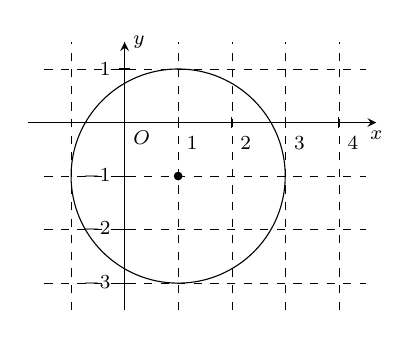
\begin{tikzpicture}[smooth,samples=300,scale=0.68,>=stealth,font=\footnotesize]
			\draw[line  width=0.1pt,dashed] (-1.5,-3.5) grid (4.5,1.5);
			\draw[->]  (-1.8,0)--(4.7,0) node[below]{$x$};
			 \draw[->] (0,-3.5)--(0,1.5) node[right]{$y$};
			\draw (0,0) node[below  right]{$O$};
			\draw (1,-1) circle  (2cm);
			\draw[fill=black] (1,-1) circle (2pt); 
			\foreach  \x in {1,2,3,4}\draw (\x,0.1)--(\x,-0.1) node [below right] {\footnotesize $\x$};
			\foreach \y in {-3,-2,-1,1}\draw (0.1,\y)--(-0.1,\y) node [left] {\footnotesize  $\y$};
		\end{tikzpicture}
	 }
	\loigiai{ 
		Đường tròn  có tâm $I(1;-1)$ và bán kính $R=2$ nên có dạng $(x-1)^2+(y+1)^2=4$.
	 }
\end{ex}

% từ: cau-hoi/lop10/0H9_Phuong_phap_toa_do_trong_mat_phang/0H9-4-2_Phuong_trinh_duong_tron.tex
\begin{bt}%[0H9H4-2]%[Dự án đề kiểm tra GHKII NH22-23 - Quang Anh]%[Trường Chinh]%[ma:fb012b63]
	\begin{enumerate}
	\item Cho đường thẳng $\Delta\colon 3x-4y+5=0$ và điểm $E(2;-1)$. Viết phương trình đường thẳng $d$ biết $d$ song song với $\Delta$ và $d$ đi qua $E$;
	\item  Xét vị trí tương đối và tìm giao điểm (nếu có) của hai đường thẳng sau:\\ $d_1\colon x+2y-2=0$; $d_2\colon 3x-y+1=0$.		
	\end{enumerate}
	\loigiai{ 
	\begin{enumerate}
		\item Vì đường thẳng $d$ song song với đường thẳng $\Delta$ nên đường thẳng $ d$ có dạng\\ $3x-4y+c=0$, với $ c\ne 5 $.	Mà $ E\in d $ nên $3\cdot2-4\cdot (-1)+c=0 \Leftrightarrow c=-10$.\\
		Vậy phương trình đường thẳng $ d\colon 3x-4y-10=0 $.
		\item Ta có $ \dfrac{1}{3}\ne\dfrac{2}{-1} $ suy ra $d_1\cap d_2={A}$, khi đó tọa độ giao điểm $A$ là nghiệm của hệ phương trình 
	\begin{eqnarray*}
		\heva{&x+2y-2=0\\&3x-y+1=0}\Leftrightarrow\heva{&x=0\\&y=1.}
	\end{eqnarray*}	
	Vậy $A(0;1)$.
	\end{enumerate}
		
	}
\end{bt}

% từ: cau-hoi/lop10/0H9_Phuong_phap_toa_do_trong_mat_phang/0H9-5-7_Xac_dinh_cac_yeu_to_cua_parabol.tex
\begin{ex}%[0H9V5-7]%[ma:a242f688]
	Trong mặt phẳng tọa độ $Oxy$, cho parabol $(P)\colon y^2=2x $ và hai điểm $ A(-3;2)$, $ B(0;-1) $. Gọi $C(a;b)$ là điểm thuộc parabol $ (P)$. Chọn khẳng định đúng, khẳng  định sai trong các khẳng định sau?
	\choiceTF 
		{\True Tọa độ của điểm  $C$ có dạng $ C\left(\dfrac{b^2}{2};b\right) $}
		 {\True Diện tích tam giác $ABC$ là $S=3\left(\dfrac{b^2}{4}+\dfrac{b}{2}+\dfrac{1}{2}\right)$}
		{\True Khi $ C\left(\dfrac{1}{2};-1\right)  $ thì tam giác $ABC$ có diện tích nhỏ nhất}
		{Khi tam giác $ABC$ cân tại $C$  thì diện tích tam giác $ABC$ đạt giá trị nhỏ nhất}
	 \loigiai{
		\begin{itemchoice}
			\itemch  Đây là khẳng định đúng vì\\
			Ta  có $ \overrightarrow{AB} =(3;-3)=3(1;-1)$.\\
			 Đường thẳng $ AB $ nhận $ \overrightarrow{u} =(1;1)$ làm một véc-tơ chỉ phương.\\
			 Suy ra đường thẳng $ AB $ nhận $ \overrightarrow{n} =(1;1)$ làm một véc-tơ pháp tuyến.\\
			Phương trình đường thẳng $ AB$ là $1\cdot (x-0)+1\cdot (y-(-1)) =0\Leftrightarrow  x+y+1=0$.\\
			Vì $ C(a;b) $ là  điểm thuộc parabol $ (P)$ nên $ b^2=2a \Rightarrow a=\dfrac{b^2}{2}$.\\
			Suy ra $  C\left(\dfrac{b^2}{2};b\right) $.\\
			 \itemch Đây là khẳng định đúng vì\\
			Diện tích tam giác $ ABC $ là 
			 \allowdisplaybreaks
			\begin{eqnarray*}
				S_{ABC}&=&\dfrac{1}{2}AB\cdot \mathrm{d}(C,AB)\\ 
				 &=&\dfrac{1}{2}\cdot \sqrt{3^2+(-3)^2}\cdot \dfrac{\left|\dfrac{b^2}{2}+b+1\right|}{\sqrt{1^2+1^2}}\\
				&=&\dfrac{3\sqrt{2}}{2}\cdot  \dfrac{\left|\dfrac{b^2}{2}+b+1\right|}{\sqrt{2}}\\
				 &=&\dfrac{3}{2}\left|\dfrac{b^2}{2}+b+1\right|=3\left(\dfrac{b^2}{4}+\dfrac{b}{2}+\dfrac{1}{2}\right).
			\end{eqnarray*}
			\itemch Đây là khẳng  định đúng vì \\
			Ta có 
			 $S_{ABC}=3\left(\dfrac{b^2}{4}+\dfrac{b}{2}+\dfrac{1}{2}\right)
			 =3\left(\left(\dfrac{b}{2}+\dfrac{1}{2}\right)^2+\dfrac{1}{4}\right)\geq 3\cdot \dfrac{1}{4}=\dfrac{3}{2}.$\\
			Ta có $ \min S_{ABC} =\dfrac{3}{2}$  đạt được khi và chỉ khi $b=-1$, $a=\dfrac{1}{2}$.\\
			Khi $  C\left(\dfrac{1}{2};-1\right) $ thì tam giác $ABC$ có diện tích nhỏ nhất.
			\itemch Đây là khẳng định sai  vì.\\
			Khi $ C\left(\dfrac{1}{2};-1\right) $ thì tam giác $ABC$  có diện tích nhỏ nhất.\\ Khi đó $CA=\dfrac{\sqrt{85}}{2}$, $CB=\dfrac{1}{2}$ nên tam giác $ABC$ không cân tại $C$.
		\end{itemchoice}
	 }
\end{ex}

% từ: cau-hoi/lop10/0H9_Phuong_phap_toa_do_trong_mat_phang/0H9-5-8_Phuong_trinh_chinh_tac_cua_parabol.tex
\begin{bt}%[0H9N5-8]%[10EX- Tex hóa CD -CT-hk2-Thầy Trịnh Xuân]%[ma:b52ccc47]
	\immini{
		Viết phương trình của parabol $(P)$ có tiêu điểm $F(3;0)$.
	}{
		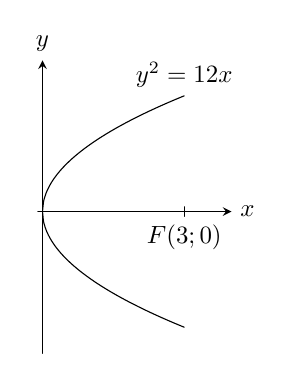
\begin{tikzpicture}[domain=0:3,line join = round, line cap = round,>=stealth,scale=0.6]
			\draw[->] (-0.1,0) -- (4,0) node[right] {$x$};
			\draw[->] (0,-3) -- (0,3.2) node[above] {$y$};
			\draw[smooth, samples=150] plot (\x,{-(2*(\x))^(0.5)});
			\draw[smooth, samples=150] plot (\x,{(2*(\x))^(0.5)}) node[above]{$y^2=12x$};
			\draw (3,0.1)--(3,-0.1) node[below]{$F(3;0)$};
		\end{tikzpicture}  
	}
	\loigiai{
		Parabol $(P)$ có tiêu điểm $F(3;0)$ nên ta có: $\dfrac{p}{2}=3$, suy ra $p=6$. Vậy $(P)$ có phương trình $y^2=12x$.
	}
\end{bt}

% từ: cau-hoi/lop11/1D1_Ham_so_luong_giac_va_phuong_trinh_luong/1D1-2-1_Cau_hoi_ly_thuyet.tex
\begin{ex}%[1D1B2-1]%[ma:3b7d7855]
	Phương trình $\sin  2x=\dfrac{\sqrt{3}}{2}$ có bao nhiêu nghiệm trên khoảng $(0;3\pi)$?
	\choice 
		{$1$} 
		{\True  $6$}
		 {$2$}
		{$4$} 
	 \loigiai{Ta có
	\[\sin  2x=\dfrac{\sqrt{3}}{2} \Leftrightarrow \hoac{&2x=\dfrac{\pi}{3}+k2\pi\\&2x=\dfrac{2\pi}{3}+k2\pi} \Leftrightarrow \hoac{&x=\dfrac{\pi}{6}+k\pi\\&x=\dfrac{\pi}{3}+k\pi}, k \in \mathbb{Z}.\]
	Khi đó 
	\begin{itemize}
		 \item Với $x=\dfrac{\pi}{6}+k\pi \in (0;3\pi) \Rightarrow k=0;~1;~2$.
		\item Với  $x=\dfrac{\pi}{3}+k\pi \in (0;3\pi) \Rightarrow k=0;~1;~2$.
	\end{itemize}
	Vậy phương trình đã cho có $6$  nghiệm thuộc $(0;3\pi)$.
	} 
\end{ex}

% từ: cau-hoi/lop11/1D1_Ham_so_luong_giac_va_phuong_trinh_luong/1D1-2-1_Cau_hoi_ly_thuyet.tex
\begin{ex}%[1D1B2-1]%[ma:8e6126e2]
	Đường thẳng $y=\dfrac{1}{2}$ cắt đồ thị hàm số $y=\cos x$ tại những  điểm có hoành độ là
	\choice 
		{\True $\pm \dfrac{\pi}{3}+k2\pi,k\in \mathbb{Z}$} 
		{$\pm  \dfrac{\pi}{6}+k2\pi,k\in \mathbb{Z}$}
		 {$\pm \dfrac{2\pi}{3}+k2\pi,k\in \mathbb{Z}$}
		{$\pm \dfrac{5\pi}{6}+k2\pi,k\in \mathbb{Z}$} 
	\loigiai{ 
		Phương trình hoành độ giao điểm $\cos x =\dfrac{1}{2}\Leftrightarrow x=\pm \dfrac{\pi}{3}+k2\pi,k\in  \mathbb{Z}$.
	 }
\end{ex}

% từ: cau-hoi/lop11/1D1_Ham_so_luong_giac_va_phuong_trinh_luong/1D1-2-2_Xet_dau_gia_tri_luong_giac_Tinh_gia_tri_luong.tex
\begin{bt}%[1D1H2-2]%[ma:a1dcffd6]
% nguon: Archive/2024/SP-K10-K11-LyVanHoang_TVN-023/11. C1-LuongGiac-lvhoang_TVN-023/dataC1K11/Bai1-Dang5.tex #1872
%[Dự án BG K10-K11]%[Dao-V- Thuy]
	Cho $90^\circ<\alpha<180^\circ$. Xét dấu các biểu thức sau:
	\begin{listEX}[2]
		\item $A=\sin (270^\circ-\alpha)$.
		\item $B=\cos (2\alpha+90^\circ)$.
	\end{listEX}
	\loigiai{
		\begin{enumerate}
			\item $A=\sin (270^\circ-\alpha)$.\\
			Vì $-180^\circ<-\alpha<-90^\circ$ nên $90^\circ<270^\circ-\alpha<180^\circ$.\\
			Do đó, điểm cuối của cung $270^\circ-\alpha$ thuộc góc phần tư thứ $\mathit{II}$ nên $A>0$.
			\item $B=\cos (2\alpha+90^\circ)$.\\
			Ta có $B=\cos (2\alpha+90^\circ)=\cos (90^\circ-(-2\alpha))=\sin(-2\alpha)=-\sin(2\alpha)$.\\
			Vì $180^\circ<2\alpha<360^\circ$ nên $\sin (2\alpha)<0$.\\
			Do đó, $B>0$.
		\end{enumerate}
	}
\end{bt}

% từ: cau-hoi/lop11/1D1_Ham_so_luong_giac_va_phuong_trinh_luong/1D1-2-3_Bien_doi_rut_gon_bieu_thuc_luong_giac_chung_m.tex
\begin{ex}[c]%[1D1H2-3]%[ma:7f6bbfde]
 Xét tính đúng - sai của  các đẳng thức sau.
  \choiceTF
  {$\sin \left(x-\dfrac{\pi}{6}\right)=\dfrac{\sqrt{3}}{2} \sin x+\dfrac{1}{2}  \cos x$}
   {\True $4 \sin x \cdot \sin 2 x \cdot \sin 3 x=\sin 4 x+\sin 2 x-\sin 6 x$}
  {$1+\sin 2 x+\cos 2 x=2 \sqrt{2} \sin  x \cdot \cos \left(x-\dfrac{\pi}{4}\right)$}
  {$\sin ^2 x+2 \sin (a-x) \cdot \sin x  \cdot \cos a+\sin ^2(a-x)=\cos ^2 a$}
 \loigiai{ 
  \begin{itemchoice}
    \itemch Sai. Theo công thức cộng ta có $$\sin \left(x-\dfrac{\pi}{6}\right)=\sin x \cdot \cos \dfrac{\pi}{6}-\cos x \cdot \sin \dfrac{\pi}{6}=\dfrac{\sqrt{3}}{2} \sin x-\dfrac{1}{2} \cos x.$$
   \itemch Đúng. Áp dụng  quy tắc từ tích sang tổng, ta được
   $$4 \sin x \cdot \sin 2 x \cdot \sin 3  x=2(\cos x-\cos 3 x) \sin 3 x=\sin 4 x+\sin 2 x-\sin 6 x.$$
   \itemch Sai. Ta có $1+\sin 2 x+\cos 2 x=2 \sin x \cos x+2 \cos ^2  x=2 \cos x\cdot (\sin x+\cos x)$.\\
   Mà $\sin x+\cos  x=\sqrt{2}\left(\cos x \dfrac{1}{\sqrt{2}}+\sin x \dfrac{1}{\sqrt{2}}\right)=\sqrt{2} \cos \left(x-\dfrac{\pi}{4}\right)$.\\
   Vậy $1+\sin 2  x+\cos 2 x=2 \sqrt{2} \cos x \cdot \cos \left(x-\dfrac{\pi}{4}\right)$.
   \itemch Sai. Ta  có
    $
   \begin{aligned}
    &\, \sin ^2 x+2 \sin (a-x)  \cdot \sin x \cdot \cos a+\sin ^2(a-x) \\
    =&\,\sin ^2 x+\sin (a-x) \cdot[\sin (x+a)+\sin (x-a)]+\sin  ^2(a-x) \\
     =&\,\sin ^2 x+\sin (a-x) \cdot[\sin (x+a)+\sin (x-a)+\sin (a-x)] \\
    =&\,\sin ^2 x+\sin (a-x) \cdot[\sin (x+a)+\sin (x-a)-\sin  (x-a)] \\
    =&\,\sin  ^2 x+\sin (a-x) \cdot \sin (x+a)\\
    =&\,\dfrac{1-\cos 2 x}{2}-\dfrac{\cos 2 a-\cos 2 x}{2}\\ 
    =&\,\dfrac{1-\cos 2 a}{2}=\sin  ^2 a .
   \end{aligned}
    $
  \end{itemchoice}
  }
\end{ex}

% từ: cau-hoi/lop11/1D1_Ham_so_luong_giac_va_phuong_trinh_luong/1D1-2-4_Cac_goc_luong_giac_co_lien_quan_dac_biet_bu_n.tex
\begin{ex}%[1D1H2-4]%[ma:7f70476f]
	Hãy  thực hiện các yêu cầu trong mỗi trường hợp sau
	\begin{enumerate}
		\item Biểu diễn $\sin \left(-\dfrac{29\pi}{3} \right)$ qua giá trị lượng giác của góc có số đo từ 0 đến $\dfrac{\pi}{4} $; 
		\item Biểu diễn tan $973^\circ $ qua giá trị  lượng giác của góc có số đo từ $0^\circ $ đến $45^\circ $.
	\end{enumerate}
	\loigiai{ 
		\begin{enumerate}
			\item  Ta có
			\begin{eqnarray*}
				\sin \left(-\dfrac{29\pi}{3} \right) &=&-\sin \left(\dfrac{29\pi}{3} \right)=-\sin  \left(\dfrac{5\pi}{3} +8\pi \right)\\
				&=& -\sin \left(\dfrac{2\pi}{3} +\pi  \right)=\sin \dfrac{2\pi}{3}\\
				&=&\cos \left(\dfrac{\pi}{2}  -\dfrac{2\pi}{3} \right)=\cos \left(-\dfrac{\pi}{6} \right)=\cos \dfrac{\pi}{6} .
			\end{eqnarray*}
			\item $\tan  973^\circ =\tan (73^\circ +5\cdot180^\circ)=\tan 73^\circ =\tan (90^\circ -17^\circ)=\cot 17^\circ $.
	\end{enumerate}}
\end{ex}

% từ: cau-hoi/lop11/1D1_Ham_so_luong_giac_va_phuong_trinh_luong/1D1-2-4_Cac_goc_luong_giac_co_lien_quan_dac_biet_bu_n.tex
\begin{bt}%[1D1V2-4]%[ma:afb2a128]
% nguon: Archive/2024/SP-K10-K11-LyVanHoang_TVN-023/11. C1-LuongGiac-lvhoang_TVN-023/dataC1K11/Bai-1-Dang-7-GTLG-GocLienQuanDacBiet.tex #1718
[MĐ3]
	Tính
	\begin{enumerate}
		\item $A=\sin ^2 5^{\circ}+\sin ^2 10^{\circ}+\sin ^2 15^{\circ}+\ldots+\sin ^2 85^{\circ}$ ($17$ số hạng).
		\item $B=\cos 5^{\circ}+\cos 10^{\circ}+\cos 15^{\circ}+\ldots+\cos 175^{\circ}$ ($35$ số hạng).
	\end{enumerate}
	\loigiai{
		\begin{enumerate}
			\item Vận dụng $\sin \left(90^{\circ}-\alpha\right)=\cos \alpha$.\\
			Ta có $\sin 85^{\circ}=\cos 5^{\circ}$,  $\sin 80^{\circ}=\cos 10^{\circ}$, $\sin 75^{\circ}=\cos 15^{\circ}, \ldots, \sin 50^{\circ}=\cos 40^{\circ}$.
			\begin{eqnarray*}
				A & =&\left(\sin ^2 5^{\circ}+\cos ^2 5^{\circ}\right)+\left(\sin ^2 10^{\circ}+\cos ^2 10^{\circ}\right)+\ldots+\left(\sin ^2 40^{\circ}+\cos ^2 40^{\circ}\right)+\sin ^2 45^{\circ} \\
				& =&\underbrace{1+1+\ldots+1}_{\text {8 số 1 }}+\left(\dfrac{\sqrt{2}}{2}\right)^2=\dfrac{17}{2} .
			\end{eqnarray*}
			\item Vận dụng $\cos \left(180^{\circ}-\alpha\right)=-\cos \alpha$.\\
			Ta có $\cos 175^{\circ}=-\cos 5^{\circ}, \cos 170^{\circ}=-\cos 10^{\circ}$, $\cos 165^{\circ}=-\cos 15^{\circ}, \ldots, \cos 95^{\circ}=-\cos 85^{\circ}$.
			\begin{eqnarray*}
				B&=&\left(\cos 5^{\circ}+\cos 175^{\circ}\right)+\left(\cos 10^{\circ}+\cos 170^{\circ}\right)+\ldots+\left(\cos 85^{\circ}+\cos 95^{\circ}\right)+\cos 90^{\circ}\\
				&=&\underbrace{0+0+\ldots+0}_{17 \text { số } 0}+\cos 90^{\circ}=0.
			\end{eqnarray*}
		\end{enumerate} 
	}
\end{bt}

% từ: cau-hoi/lop11/1D1_Ham_so_luong_giac_va_phuong_trinh_luong/1D1-3-3_Ap_dung_cong_thuc_nhan_doi_ha_bac.tex
\begin{ex}%[1D1H3-3]%[ma:8d083f77]
	Cho $\sin 2\alpha =\dfrac {3}{4}$. Tính giá trị biểu thức  $A=\tan \alpha +\cot \alpha$.
	\choice 
		{$A=\dfrac  {4}{3}$}
		{$A=\dfrac {2}{3}$} 
		 {\True $A=\dfrac {8}{3}$}
		 {$A=\dfrac {16}{3}$}
	\loigiai{ 
		\allowdisplaybreaks 
		\begin{align*}
			A&=\tan \alpha +\cot \alpha\\ 
			&=\dfrac {\sin \alpha}{\cos \alpha}+\dfrac {\cos \alpha}{\sin \alpha}\\ 
			&=\dfrac {\sin^2\alpha +\cos^2\alpha }{\sin \alpha \cos  \alpha}\\
			&=\dfrac  {1}{\dfrac {1}{2}\sin 2\alpha}\\
			&=\dfrac {1}{\dfrac {1}{2}\cdot \dfrac {3}{4}}\\ 
			&=\dfrac  {8}{3}.
		\end{align*}
	 }
\end{ex}

% từ: cau-hoi/lop11/1D1_Ham_so_luong_giac_va_phuong_trinh_luong/1D1-3-3_Ap_dung_cong_thuc_nhan_doi_ha_bac.tex
\begin{bt}%[1D1N3-3]%[ma:63fdcca7]
% nguon: Archive/SP_KhoLatex/ID6_old/1K1-2.tex #3593
%[Dự án 1 - TLDH - TeamTeXHoa - Huỳnh Xuân Tín]
	Cho $\dfrac{1}{\tan ^2 \alpha}+\dfrac{1}{\cot ^2 \alpha}+\dfrac{1}{\sin ^2 \alpha}+\dfrac{1}{\cos ^2 \alpha}=7$. Tính $\cos 4 \alpha$.	
	\loigiai{Ta có
		$$
		\begin{aligned}
		&\dfrac{1}{\tan ^2 \alpha}+\dfrac{1}{\cot ^2 \alpha}+\dfrac{1}{\sin ^2 \alpha}+\dfrac{1}{\cos ^2 \alpha}=7 \\
		& \Leftrightarrow \dfrac{\sin ^2 \alpha+1}{\cos ^2 \alpha}+\dfrac{\cos ^2 \alpha+1}{\sin ^2 \alpha}=7 \\
		& \Leftrightarrow \dfrac{\sin ^2 \alpha\left(\sin ^2 \alpha+1\right)+\cos ^2 \alpha\left(\cos ^2 \alpha+1\right)}{\sin ^2 \alpha \cos ^2 \alpha}=7 \\
		& \Leftrightarrow \sin ^4 \alpha+\cos ^4 \alpha+1=7 \sin ^2 \alpha \cos ^2 \alpha \\
		& \Leftrightarrow\left(\sin ^2 \alpha+\cos ^2 \alpha\right)^2-2 \sin ^2 \alpha \cos ^2 \alpha+1=7 \sin ^2 \alpha \cos ^2 \alpha \\
		& \Leftrightarrow 2=9 \sin ^2 \alpha \cos ^2 \alpha \\
		& \Leftrightarrow 8=9(2 \sin \alpha \cos \alpha)^2 \\
		& \Leftrightarrow 8=9 \sin ^2 2 \alpha \\
		& \Leftrightarrow 16=9(1-\cos 4 \alpha) \\
		& \Leftrightarrow \cos 4 \alpha=-\dfrac{7}{9}.
		\end{aligned}
		$$
		Vậy $\cos 4 \alpha=-\dfrac{7}{9}$.		
	}	
\end{bt}

% từ: cau-hoi/lop11/1D1_Ham_so_luong_giac_va_phuong_trinh_luong/1D1-3-4_Ap_dung_cong_thuc_bien_doi_tich_tong.tex
\begin{ex}%[1D1N3-4]%[ma:3b0fc677]
	Rút gọn biểu thức $A = \dfrac{1 + \sin 4\alpha - \cos 4\alpha}{1 + \sin 4\alpha  + \cos 4\alpha}$.
	\choice 
		{$\sin  2\alpha$}
		{$\cos 2\alpha$} 
		{\True $\tan 2\alpha$} 
		 {$\cot 2\alpha$}
	\loigiai{ 
		Ta có  \\
		$A = \dfrac{(1-\cos 4\alpha)+\sin 4\alpha}{(1+\cos 4\alpha)+\sin 4\alpha} = \dfrac{2\sin^2 2\alpha+2\sin  2\alpha\cos 2\alpha}{2\cos^2 2\alpha+2\sin 2\alpha\cos 2\alpha} = \dfrac{2\sin 2\alpha(\sin 2\alpha+\cos 2\alpha)}{2\cos 2\alpha(\sin 2\alpha+\cos 2\alpha)} = \tan 2\alpha$.
	} 
\end{ex}

% từ: cau-hoi/lop11/1D1_Ham_so_luong_giac_va_phuong_trinh_luong/1D1-3-5_Ket_hop_nhieu_cong_thuc_luong_giac.tex
\begin{ex}%[1D1H3-5]%[ma:ababe10f]
	Biết $\tan\alpha=2$. Khi  đó
	 \choiceTF
		{$\cot\alpha=-\dfrac{1}{2}$} 
		 {\True $\cos 2\alpha=-\dfrac{3}{5}$}
		{\True $\sin  2\alpha=\dfrac{4}{5}$}
		 {\True $\tan 2\alpha=-\dfrac{4}{3}$}
	 \loigiai{
		Ta  có
		\begin{itemize}
			\item $\cos 2\alpha=2\cos  ^2\alpha-1=\dfrac{2}{\tan^2\alpha+1}-1=\dfrac{2}{5}-1=-\dfrac{3}{5}$. \item $\sin 2\alpha=2\sin\alpha\cos\alpha=2\tan\alpha{\cos ^2}\alpha=\dfrac{2\tan\alpha}{\tan^2\alpha+1}=\dfrac{4}{5}$.
			\item $\tan 2\alpha=\dfrac{\sin 2\alpha}{\cos  2\alpha}=-\dfrac{4}{3}$.
		\end{itemize}
	 }
\end{ex}

% từ: cau-hoi/lop11/1D1_Ham_so_luong_giac_va_phuong_trinh_luong/1D1-3-5_Ket_hop_nhieu_cong_thuc_luong_giac.tex
\begin{ex}%[1D1V3-5]%[ma:cf54db80]
	Cho góc $\alpha$ thỏa  mãn $-\dfrac{\pi}{2}<\alpha<0$ và $\cot{\alpha}=-3$.
	\choiceTF 
		{$\sin{\alpha}>0$} 
		 {\True $\sin{\alpha}=-\dfrac{\sqrt{10}}{10}$}
		{\True  $\dfrac{\cos{\alpha}-\sin{\alpha}}{\cos^3{\alpha}+3\sin^3{\alpha}+2\cos{\alpha}}=\dfrac{10}{21}$}
		{\True $\left[\tan{\dfrac{17\pi}{4}}+\tan{\left(\dfrac{7\pi}{2}-\alpha\right)}\right]^2+\left[\cot{\dfrac{13\pi}{4}}+\cot{(7\pi-\alpha)}\right]^2=20$} 
	\loigiai{ 
	Ta có  $1+\cot^2{\alpha}=\dfrac{1}{\sin^2{\alpha}}\Rightarrow\sin^2{\alpha}=\dfrac{1}{1+\cot^2{\alpha}}=\dfrac{1}{1+(-3)^2}=\dfrac{1}{10}$.\\
	Mà $-\dfrac{\pi}{2}<\alpha<0$  nên suy ra $\sin{\alpha}=-\dfrac{\sqrt{10}}{10}$.\\
	 Đặt $P=\dfrac{\cos{\alpha}-\sin{\alpha}}{\cos^3{\alpha}+3\sin^3{\alpha}+2\cos{\alpha}}$.\\
	Chia cả tử và mẫu của $P$ cho  $\sin^3{\alpha}$, ta được
	\[P=\dfrac{\dfrac{\cos{\alpha}}{\sin^3{\alpha}}-\dfrac{1}{\sin^2{\alpha}}}{\dfrac{\cos^3{\alpha}}{\sin^3{\alpha}}+3+2\dfrac{\cos{\alpha}}{\sin^3{\alpha}}}=\dfrac{\cot{\alpha}\left(1+\cot^2{\alpha}\right)-\left(1+\cot^2{\alpha}\right)}{\cot^3{\alpha}+3+2\cot{\alpha}\left(1+\cot^2{\alpha}\right)}=\dfrac{10}{21}.\] 
	Ta có 
	\begin{itemize}
		\item $\tan{\dfrac{17\pi}{4}}=\tan{\left(\dfrac{\pi}{4}+4\pi\right)}=\tan{\dfrac{\pi}{4}}=1;  \tan{\left(\dfrac{7\pi}{2}-\alpha\right)}=\cot{\alpha}$.
		 \item $\cot{\left(\dfrac{13\pi}{4}\right)}=\cot{\left(\dfrac{\pi}{4}+3\pi\right)}=\cot{\dfrac{\pi}{4}}=1; \cot{(7\pi-\alpha)}=-\cot{\alpha}$.
	\end{itemize}
	Khi đó 
	\begin{align*}
		&\,\left[\tan{\dfrac{17\pi}{4}}+\tan{\left(\dfrac{7\pi}{2}-\alpha\right)}\right]^2+\left[\cot{\dfrac{13\pi}{4}}+\cot{(7\pi-\alpha)}\right]^2\\ 
		 &\,=\left(1+\cot{\alpha}\right)^2+\left(1-\cot{\alpha}\right)^2\\
		 &\,=2+2\cot^2{\alpha}=2+2\cdot(-3)^2=20.
	\end{align*}
	} 
\end{ex}

% từ: cau-hoi/lop11/1D1_Ham_so_luong_giac_va_phuong_trinh_luong/1D1-3-5_Ket_hop_nhieu_cong_thuc_luong_giac.tex
\begin{ex}%[1D1H3-5]%[ma:bb4d5a54]
	 Cho $\cot\alpha=3$. Tính $A=\dfrac{3\sin\alpha-2\cos\alpha}{12\sin^3\alpha+4\cos^3\alpha}$.
	 \shortans{0,25}
	 \loigiai{
		 Ta có
		 $A=\dfrac{3\sin\alpha-2\cos\alpha}{12\sin^3\alpha+4\cos^3\alpha}=\dfrac{\dfrac{1}{\sin^2\alpha}(3-2\cot\alpha)}{12+4\cot^3\alpha}=\left(1+\cot^2\alpha\right)\dfrac{3-2\cot\alpha}{12+4\cot^3\alpha}=-\dfrac{1}{4}$.
	} 
\end{ex}

% từ: cau-hoi/lop11/1D1_Ham_so_luong_giac_va_phuong_trinh_luong/1D1-3-5_Ket_hop_nhieu_cong_thuc_luong_giac.tex
\begin{ex}%[1D1H3-5]%[ma:d915def2]
	Cho $\tan\alpha=2$ .  Tính $C=\dfrac{\sin\alpha}{\sin^3\alpha+2\cos^3\alpha}$.
	\shortans{1} 
	\loigiai{ 
		Tacó  $C=\dfrac{\sin\alpha}{\sin^3\alpha+2\cos^3\alpha}=\dfrac{\tan\alpha\cdot\dfrac{1}{\cos^2\alpha}}{\tan^3\alpha+2}=\dfrac{\tan\alpha\left(1+\tan^2\alpha\right)}{\tan^3\alpha+2}=\dfrac{2\left(1+2^2\right)}{2^3+2}=1$.
	 }
\end{ex}

% từ: cau-hoi/lop11/1D1_Ham_so_luong_giac_va_phuong_trinh_luong/1D1-4-4_Xet_tinh_chan_le.tex
\begin{bt}%[1D1H4-4]%[ma:fda1ef9b]
% nguon: Archive/SP_KhoLatex/ID6_old/1K1-3.tex #3553
%[Dự án 1 - TLDH - TeamTeXHoa - Trần Trọng Tiên]
	Xét tính chẵn lẻ của các hàm số sau:
	\begin{listEX}[2]
		\item $y=\sin 2x+\tan 2x$;
		\item $y=\cos x+\sin^2x$;
		\item $y=\sin x\cos 2x$;
		\item $y=\sin x+\cos x$.
	\end{listEX}
	\loigiai{
		\begin{listEX}[1]
			\item Biểu thức $\sin 2x+\tan 2x$ có nghĩa khi $\cos 2x\ne 0$ $\left(\text{do } \tan 2x=\dfrac{\sin 2x}{\cos 2x}\right)$, tức là 
			\[2x\ne \dfrac{\pi}{2}+k\pi,~k\in\mathbb{Z}\Leftrightarrow x\ne\dfrac{\pi}{4}+k\dfrac{\pi}{2},~k\in\mathbb{Z}.\]
			Suy ra tập xác định của hàm số $y=f(x)=\sin 2x+\tan 2x$ là $\mathscr{D}=\mathbb{R}\setminus \left\{\dfrac{\pi}{4}+k\dfrac{\pi}{2}\big |k\in\mathbb{R}\right\}$.\\
			Do đó, nếu $x$ thuộc tập xác định $\mathscr{D}$ thì $-x$  cũng thuộc tập xác định $\mathscr{D}$. Ta có\\
			$f(-x)=\sin(-2x)+\tan(-2x)=-\sin 2x-\tan 2x=-(\sin 2x+\tan 2x)=-f(x)$, với mọi $x$ thuộc $\mathscr{D}$.\\
			Vậy $y=\sin 2x+\tan 2x$ là hàm số lẻ.
			\item Tập xác định của hàm số $y=\cos x+\sin^2x$ là $\mathscr{D}=\mathbb{R}$.\\
			Do đó, nếu $x$ thuộc tập xác định $\mathscr{D}$ thì $-x$ cũng thuộc tập xác định $\mathscr{D}$.\\
			Ta có $f(-x)=\cos(-x)+\sin^2(-x)=\cos x+(\sin x)^2=\cos x+\sin^2x=f(x),~\forall x\in\mathscr{D}$.\\
			Vậy $y=\cos x+\sin^2 x$ là hàm số chẵn.	
			\item Tập xác định của hàm số $y=\sin x\cos 2x$ là $\mathscr{D}=\mathbb{R}$.\\
			Do đó, nếu $x$ thuộc tập xác định $\mathscr{D}$ thì $-x$ cũng thuộc tập xác định $\mathscr{D}$.\\
			Ta có $f(-x)=\sin (-x)\cdot\cos (-2x)=-\sin x\cdot\cos 2x= -f(x),~\forall x\in\mathscr{D}$.\\
			Vậy $y=\sin x\cos 2x$  là hàm số lẻ.
			\item Tập xác định của hàm số $y=\sin x+\cos x$ là $\mathscr{D}=\mathbb{R}$.\\
			Do đó, nếu $x$ thuộc tập xác định $\mathscr{D}$ thì $-x$ cũng thuộc tập xác định $\mathscr{D}$.\\
			Ta có $f(-x)=\sin (-x)+\cos (-x)=-\sin x+\cos x\ne-f(x)$.\\
			Vậy $y=\sin x+\cos x$  là hàm số không chẵn, không lẻ.
		\end{listEX}
	}
\end{bt}

% từ: cau-hoi/lop11/1D1_Ham_so_luong_giac_va_phuong_trinh_luong/1D1-4-5_Xet_tinh_tuan_hoan_tim_chu_ky.tex
\begin{bt}%[1D1V4-5]%[ma:a980fac5]
% nguon: Archive/SP_KhoLatex/ID6_old/1K1-3.tex #3548
%[Dự án 1 - TLDH - TeamTeXHoa - Trần Trọng Tiên]
	Xét tính tuần hoàn và tìm chu kỳ cơ sở (nếu có) của các hàm số sau
	\begin{listEX}[2]
		\item $f(x)=\cos\dfrac{3x}{2}\cos\dfrac{x}{2}$;
		\item $y=\cos x+\cos \left(\sqrt{3}x\right)$;
		\item $f(x)=\sin \left(x^2\right)$;
		\item $y=\tan \sqrt{x}$.
	\end{listEX}
	\loigiai{
		\begin{listEX}[1]
			\item Ta có $f(x)=\cos\dfrac{3x}{2}\cos\dfrac{x}{2}=\dfrac{1}{2}\left[\cos\left(\dfrac{3x}{2}+\dfrac{x}{2}\right)+\cos \left(\dfrac{3x}{2}-\dfrac{x}{2}\right)\right]=\dfrac{1}{2}\left(\cos 2x+\cos x\right)$.
			\begin{itemize}
				\item 	Hàm số $f(x)=\cos 2x$ tuần hoàn với chu kì $\dfrac{2\pi}{2}=\pi$.
				\item Hàm số $f(x)=\cos x$ tuần hoàn với chu kì $\dfrac{2\pi}{1}=2\pi$.
			\end{itemize}
			Vậy hàm số $f(x)=\cos\dfrac{3x}{2}\cos\dfrac{x}{2}$ tuần hoàn với chu kì $T$ là bội chung nhỏ nhất của $\pi$ và $2\pi$, do đó $T=2\pi$.
			\item Giả sử hàm số đã cho tuần hoàn, suy ra có số thực dương $T$ thỏa:
			\[f(x+T)=f(x)\Leftrightarrow \cos(x+T)+\cos\sqrt{3}(x+T)=\cos x+\cos\sqrt{3}x.\]
			Cho $x=0\Rightarrow \cos T+\cos \sqrt{3} T=2\Leftrightarrow\heva{&\cos T=1\\&\cos \sqrt{3} T=1}\Rightarrow \heva{&T=2n\pi\\&\sqrt{3}T=2m\pi}$\\
			$\Rightarrow \sqrt{3}=\dfrac{m}{n}$ (vô lí do $m,n\in\mathbb{Z}\Rightarrow \dfrac{m}{n}$ là số hữu tỉ).\\
			Vậy hàm số đã cho không tuần hoàn.
			\item Hàm số  $f(x)=\sin \left(x^2\right)$ không tuần hoàn vì khoảng cách giữa các nghiệm (không điểm) liên tiếp của nó dần tới $0$
			\[\sqrt{(k+1) \pi}-\sqrt{k \pi}=\dfrac{\pi}{\sqrt{(k+1) \pi}+\sqrt{k \pi}} \rightarrow 0 \text{ khi } k\rightarrow \infty.\]
			\item Hàm số $y=\tan \sqrt{x}$ không tuần hoàn vì khoảng cách giữa các nghiệm (không điểm) liên tiếp của nó dần tới $0$
			\[(k+1)^2 \pi^2-k^2 \pi \rightarrow \infty \text{ khi }k \rightarrow \infty.\]
		\end{listEX}
	}
\end{bt}

% từ: cau-hoi/lop11/1D1_Ham_so_luong_giac_va_phuong_trinh_luong/1D1-4-6_Tim_tap_gia_tri_va_min_max.tex
\begin{ex}%[1D1H4-6]%[ma:cad220bb]
	Tìm tập giá trị của  các hàm số sau đây
	\begin{listEX}[2]
		 \item $y=2\sin\left(x-\dfrac{\pi}{4} \right)-1$.
		\item  $y=\sqrt{1+\cos x}-2$.
	\end{listEX}
	 \loigiai{
		\begin{enumerate}
			 \item Ta có \allowdisplaybreaks
			\begin{eqnarray*}
				&&-1\le \sin\left(x-\dfrac{\pi}{4} \right)\le 1,\,\forall x\in  \mathbb{R}\\
				&\Leftrightarrow& -2\le 2\sin\left(x-\dfrac{\pi}{4} \right)\le 2,\, \forall  x\in \mathbb{R}\\
				&\Leftrightarrow& -2-1\le 2\sin\left(x-\dfrac{\pi}{4} \right)-1\le  2-1,\, \forall x\in \mathbb{R}\\
				&\Leftrightarrow& -3\le 2\sin\left(x-\dfrac{\pi}{4}  \right)-1\le 1,\, \forall x\in \mathbb{R}\\
				&\Leftrightarrow& -3\le y\le 1,\, \forall x\in \mathbb{R}. 
			\end{eqnarray*}
			Vậy tập giá trị  của hàm số $y=2\sin\left(x-\dfrac{\pi}{4} \right)-1$ là $\left[-3;1\right]$
			\item Vì $-1\le \cos x\le 1$, $\forall x\in \mathbb{R}$ nên  $0\le 1+\cos x\le 2$, $\forall x\in \mathbb{R}$.\\
			Do đó $0\le \sqrt{1+\cos x} \le \sqrt{2}$, $\forall x\in \mathbb{R}$.\\ Suy ra $-2\le \sqrt{1+\cos x}-2\le \sqrt{2}-2$, $\forall x\in \mathbb{R}$.  \\
			Hay $-2\le y\le \sqrt{2}-2$,  $\forall x\in \mathbb{R}$.\\
			Vậy tập giá trị của hàm số $y=\sqrt{1+\cos x}-2$ là  $\left[-2;\sqrt{2}-2\right]$.
		\end{enumerate}
	} 
\end{ex}

% từ: cau-hoi/lop11/1D1_Ham_so_luong_giac_va_phuong_trinh_luong/1D1-4-6_Tim_tap_gia_tri_va_min_max.tex
\begin{bt}%[1D1V4-6]%[ma:b5b40c15]
% nguon: Archive/SP_KhoLatex/ID6_old/1K1-2.tex #3606

	Tìm giá trị nhỏ nhất, lớn nhất của biểu thức sau
	\begin{listEX}[2]
		\item $A=\sin x+\cos x$.
		\item $B=\sin^4x+\cos^4x$.
	\end{listEX}
	\loigiai{
		\begin{enumerate}
			\item Ta có $A^2=\left( \sin x+\cos x \right)^2=\sin^2x+\cos^2x+2\sin x\cos x=1+\sin 2x$.\\
			Vì $\sin 2x\le 1$ nên $A^2=1+\sin 2x\le 1+1=2$ suy ra $-\sqrt{2}\le A\le \sqrt{2}$.\\
			Khi $x=\dfrac{\pi }{4}$ thì $A=\sqrt{2}$, $x=-\dfrac{3\pi }{4}$ thì $A=-\sqrt{2}$.\\
			Do đó $\max A=\sqrt{2}$ và $\min A=-\sqrt{2}$.
			\item Ta có 
			\begin{eqnarray*}
				B &=& \left( \dfrac{1-\cos 2x}{2} \right)^2+\left( \dfrac{1+\cos 2x}{2} \right)^2\\
				&=& \dfrac{1-2\cos 2x+\cos^22x}{4}+\dfrac{1+2\cos 2x+\cos^22x}{4}\\
				&=& \dfrac{2+2\cos^2 2x}{4}=\dfrac{2+1+\cos 4x}{4}=\dfrac{3}{4}+\dfrac{1}{4}\cdot\cos 4x.
			\end{eqnarray*}
			Vì $-1\le \cos 4x\le 1$ nên $\dfrac{1}{2}\le \dfrac{3}{4}+\dfrac{1}{4}\cdot\cos 4x\le 1$ suy ra $\dfrac{1}{2}\le B\le 1$.\\
			Vậy $\max B=1$ khi $\cos 4x=1$ và $\min B=\dfrac{1}{2}$ khi $\cos 4x=-1$.
		\end{enumerate}
	}
\end{bt}

% từ: cau-hoi/lop11/1D1_Ham_so_luong_giac_va_phuong_trinh_luong/1D1-4-7_Bang_bien_thien_va_do_thi.tex
\begin{bt}%[1D1H4-7]%[ma:06a18539]
% nguon: Archive/SP_KhoLatex/ID6_old/1K1-3.tex #3549
%[Dự án 1 - TLDH - TeamTeXHoa]
	Vẽ đồ thị hàm số $y=\sin 4x$.
	\loigiai{
		Miền xác định: $\mathscr{D}=\mathbb{R}$.\\
		Ta chỉ cần vẽ đồ thị hàm số trên miền $\left[0 ; \dfrac{\pi}{2}\right]$ (do chu kì tuần hoàn $T=\dfrac{2\pi}{4}=\dfrac{\pi}{2}$).\\
		Bảng giá trị của hàm số $y=\sin 4x$ trên đoạn $\left[0 ; \dfrac{\pi}{2}\right]$ là
		\begin{center}
			\setlength\extrarowheight{10pt}
			\begin{tabular}{|c|c|c|c|c|c|c|c|c|c|c|}
				\hline
				$x$	& $0$ &$\dfrac{\pi}{16}$  & $\dfrac{\pi}{8}$ & $\dfrac{3\pi}{16}$ & $\dfrac{5\pi}{24}$ & $\dfrac{\pi}{4}$ & $\dfrac{5\pi}{16}$ & $\dfrac{3\pi}{8}$ &$\dfrac{\pi}{3}$  & $\dfrac{\pi}{2}$ \\
				\hline
				$y$	& $0$  & $\dfrac{\sqrt{2}}{2}$ & $1$ & $\dfrac{\sqrt{2}}{2}$ & $\dfrac{\sqrt{3}}{2}$ & $0$  & $-\dfrac{\sqrt{2}}{2}$ & $-1$ & $-\dfrac{\sqrt{3}}{2}$ &  $0$\\
				\hline
			\end{tabular}
		\end{center}
		Ta có đồ thị của hàm số $y=\sin 4x$ trên đoạn  $\left[0 ; \dfrac{\pi}{2}\right]$ và sau đó tịnh tiến cho các đoạn: $\ldots,\left[-\dfrac{\pi}{2} ; 0\right],\left[\dfrac{\pi}{2} ; \pi\right],\ldots$
	}
	\begin{center}
		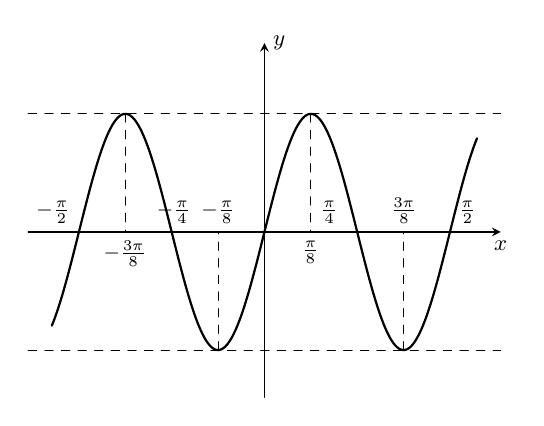
\begin{tikzpicture}[scale=1.5, font=\footnotesize, line join=round, line cap=round, >=stealth]
			\draw[->] (-2,0) -- (2,0) node[below] {\small $x$};
			\draw[->] (0,-1.4)-- (0,1.6) node[right] {\small $y$};
			\draw[thick,samples=300,domain=-1.8:1.8] plot(\x,{sin((4*\x)*180/pi)});
			\draw[dashed] (0.39,1)--(0.39,0) node[below] {$\frac{\pi}{8}$};
			\draw[dashed] (-0.39,-1)--(-0.39,0) node[above] {$-\frac{\pi}{8}$};
			\draw (-0.55,0) node[above left] {$-\frac{\pi}{4}$};	
			\draw (0.4,0) node[above right] {$\frac{\pi}{4}$};	
			\draw (-1.57,0) node[above left] {$-\frac{\pi}{2}$};
			\draw (1.57,0) node[above right] {$\frac{\pi}{2}$};	
			\draw[dashed] (-1.18,1)--(-1.18,0) node[below] {$-\frac{3\pi}{8}$};
			\draw[dashed] (1.18,-1)--(1.18,0) node[above] {$\frac{3\pi}{8}$};	
			\draw[dashed] (-2,1)--(2,1);
			\draw[dashed] (-2,-1)--(2,-1);
		\end{tikzpicture}	
	\end{center}
\end{bt}

% từ: cau-hoi/lop11/1D1_Ham_so_luong_giac_va_phuong_trinh_luong/1D1-4-8_Toan_thuc_te_ap_dung_ham_so_luong_giac.tex
\begin{ex}%[1D1V4-8]%[ma:dfc0e75c]
	\immini{Khi đu quay hoạt động, vận tốc theo phương ngang của một cabin $M$ phụ thuộc vào góc lượng giác $\alpha = \left(Ox,OM\right)$ theo hàm số $v_x = 0{,}5\sin\alpha$ (m/s).  Giá trị lớn nhất của $ v_x $ là
	 }{\resizebox{!}{4.5cm}{
	\begin{tikzpicture}[font=\small,line join=round,line cap=round,>=stealth]
			\tikzset{declare function={g=0;}} 
			 \coordinate (O) at (0,0);
			 \pgfmathsetmacro{\gx}{60-g};
			 \draw (O) circle (4.4)
				(O)  circle (3.53);
			\foreach \t in {0,1,...,11}{ 
				\draw[very thick,fill] (O)--(g+30*\t:4.4) circle  (0.06);
				\begin{scope}[shift={(g+30*\t:4.4)}]
				\draw[fill=teal] (-0.27,0)--(0.27,0)--(0.36,-0.18)--(-0.36,-0.18)--cycle 
				 (0.32,-0.18)--(0.32,-0.54)
				(-0.32,-0.18)--(-0.32,-0.54) 
				 (-0.4,-0.54)--(0.4,-0.54)--(0.27,-1)--(-0.27,-1)--cycle;
				\end{scope}}
			\draw[fill=gray!70!yellow]  (0.2,0)--(2.35,-5.53)--(3.65,-5.53)--(3.65,-6.02)--(1.95,-6.02)--(0,-0.85)--(-1.95,-6.02)--(-3.65,-6.02)--(-3.65,-5.53)--(-2.35,-5.53)--(-0.2,0)--cycle;
			\draw[fill=gray!10!yellow] (O) circle  (0.34);
			 \draw[fill] (-5,-5.85)--(0,-5.85) circle (0.08)--(6.4,-5.85);
			 \draw[->] (-5,0)--(6.7,0) node [below]{\color{black}$x$};
			\path 
				(3.82,2.22) coordinate (M) 
				($(M)-(1.8,0)$) coordinate  (N)
				 ($(N)+(0,2.5)$) coordinate (P);
			\fill[black] (M) circle (1pt)  node[above right]{$M$};
			\fill[black]  (N) circle (0pt) node[below left]{$\overrightarrow{v}_x$};
			\fill[black] (P) circle (0pt)  node[above]{$\overrightarrow{v}$};
			 \fill[black] (O) circle (1pt);
			\fill[black] (O)+(-90:0.3) circle (0pt) node[below]{$O$}; 
			\draw[->] (M)--(N); 
			\draw[->] (M)--(P); 
			\draw[dashed]  (N)--(P);
			\draw  (O)--(M);
			\draw[->] (O)+(0:0.8) arc (0:30:0.8) node[below right]{$\alpha$}; 
			 \draw pic[draw,angle radius = 4mm] {right angle=O--M--P};
		\end{tikzpicture}
	}} 
	 \shortans{0,5}
	 \loigiai{ Với mọi $ \alpha $ ta có\\
		$ -1\le \sin\alpha \le 1 \Rightarrow -0{,}5\le 0{,}5\sin\alpha \le 0{,}5 \Rightarrow -0{,}5 \le  v_x \le 0{,}5$.\\
		Vậy giá trị lớn  nhất của $v_x$ là $0{,}5$ (m/s).
	 }
\end{ex}

% từ: cau-hoi/lop11/1D1_Ham_so_luong_giac_va_phuong_trinh_luong/1D1-4-8_Toan_thuc_te_ap_dung_ham_so_luong_giac.tex
\begin{bt}%[1D1V4-8]%[ma:985f243b]
% nguon: Archive/2024/SP-K10-K11-LyVanHoang_TVN-023/11. C1-LuongGiac-lvhoang_TVN-023/dataC1K11/Bai-3-Dang-6-Dothihamsoluonggiac.tex #2063
%[BG K11, Nhật Thiện]
	[Mức độ 3]
	Trong hình vẽ bên dưới, một chiếc máy bay $A$ bay ở độ cao $500$ m theo một đường thẳng đi ngang qua phía trên trạm quan sát $T$ ở mặt đất. Hình chiếu vuông góc của $A$ lên mặt đất là $H$, $\alpha$ là góc lượng giác $\left(Tx,TA\right)$ $\left(0<\alpha<\pi\right)$.
	\begin{center}
		\begin{tikzpicture}[>=stealth,x=1.0cm,y=1.0cm, scale=1]
			\draw[->](0,0) -- (14,0) node[below]{\footnotesize $x$ (m)};
			\draw[dashed,red](0,3) -- (14,3);
			\path
			(5,0) coordinate (T)
			(10,0) coordinate (H)
			(10,3) coordinate (A)
			;
			\draw[fill = black] (T) node [below]{\footnotesize$T$ (trạm quan sát)} circle (1pt) -- (H) node [below] {\footnotesize$H$} circle (1pt) -- (A) node [above]{\footnotesize$A$ (máy bay)} circle (1pt) -- (T);
			\draw (10,1.5) node [right]{\footnotesize $500$m};
			\draw pic[->,draw, angle radius=5mm]{angle=H--T--A} (T) node[shift={(10:.8)}]{$\alpha$};
			\path pic[draw,angle radius=6]{right angle=A--H--T};
		\end{tikzpicture}
	\end{center}
	\begin{enumerate}
		\item Biểu diễn tọa độ $x_H$ của điểm $H$ trên trục $Tx$ theo $\alpha$.
		\item Dựa vào đồ thị hàm số cô-tang, hãy cho biết với $\dfrac{\pi}{6} < \alpha < \dfrac{2\pi}{3}$ thì $x_H$ nằm trong khoảng nào? Làm tròn kết quả đến hàng phần mười.
	\end{enumerate}
	\loigiai{
		\begin{enumerate}
			\item Coi trạm quan sát $T$ là gốc tọa độ thì ta có
			\[x_H = \overline{TH} = AH\cdot\cot\alpha = 500\cot\alpha\;\left(\text{m}\right).\]
			\item \immini{
				Dựa vào đồ thị hàm số $\cot x$, ta thấy với $\dfrac{\pi}{6} < \alpha < \dfrac{2\pi}{3}$ thì $-\dfrac{\sqrt{3}}{3} < \cot \alpha < \sqrt{3}$.\\
				Do đó $-\dfrac{500\sqrt{3}}{3} < x_H < 500\sqrt{3}$. Làm tròn kết quả đến hàng phần mười ta được
				\[-288{,}7 < x_H< 866{,}0.\]
			}{
				\begin{tikzpicture}[font=\footnotesize,line join = round, line cap = round,>=stealth,scale=1]
					\draw[->] (-1,0) -- (4,0.)node[below]{\footnotesize $x$};
					\draw[->] (0,-3.1) -- (0,4.25)node[left]{\footnotesize $y$};
					\draw (0,0) node[above left] {\footnotesize $O$};
					\draw[dashed,smooth,samples=100,domain=0.25:2.8] plot(\x,{cot(((\x))*180/pi)});
					\draw[line width=1pt,smooth,red,samples=100,domain=pi/6:2*pi/3] plot(\x,{cot(((\x))*180/pi)});
					\draw[dashed] (pi,-3.1) -- (pi,0) node[below right]{$\pi$} -- (pi,4.2);
					\draw[dashed] (pi/6,0) node[below]{$\tfrac{\pi}{6}$} circle (1pt) --(pi/6,1.73)--(0,1.73) node[left]{$\sqrt{3}$};
					\draw[dashed] (2*pi/3,0) node[above]{$\tfrac{2\pi}{3}$} circle (1pt) --(2*pi/3,-0.577)--(0,-0.577) node[left]{$-\tfrac{\sqrt{3}}{3}$};
				\end{tikzpicture}
			}
		\end{enumerate}
	}
\end{bt}

% từ: cau-hoi/lop11/1D1_Ham_so_luong_giac_va_phuong_trinh_luong/1D1-4-8_Toan_thuc_te_ap_dung_ham_so_luong_giac.tex
\begin{bt}%[1D1V4-8]%[ma:7220b941]
% nguon: Archive/2025-Sangtac/Khoi11/Data/1-CTST/CTST_1-OTGK1_De04.tex #5014

	\immini{Khi đu quay hoạt động, vận tốc theo phương ngang của một cabin $M$ phụ thuộc vào góc lượng giác $\alpha = \left(Ox,OM\right)$ theo hàm số $v_x = 0{,}5\sin\alpha$ (m/s). Giá trị lớn nhất của $ v_x $ là}
	{
		\begin{tikzpicture}[scale=0.6,font=\small,line join=round,line cap=round,>=stealth]
			\tikzset{declare function={g=0;}}
			\coordinate (O) at (0,0);
			%	\coordinate[label=above right:$A$] (A) at (0:4.4);
			%	\coordinate[label=above right:$M$] (M) at (30+g:4.4);
			\pgfmathsetmacro{\gx}{60-g};
			\coordinate (v) at ($(M)+(120+g:3.3)$);
			\coordinate (vx) at ($(M)+(180:3.3*cos \gx)$);
			\draw[thick] (O) circle(4.4) (O) circle(3.53);
			\foreach \t in {0,1,...,11}{
				\draw[very thick,fill] (O)--(g+30*\t:4.4)circle(0.06);
				\begin{scope}[shift={(g+30*\t:4.4)}]
					\draw[fill=teal] (-0.27,0)--(0.27,0)--(0.36,-0.18)--(-0.36,-0.18)--cycle
					(0.32,-0.18)--(0.32,-0.54) (-0.32,-0.18)--(-0.32,-0.54)
					(-0.4,-0.54)--(0.4,-0.54)--(0.27,-1)--(-0.27,-1)--cycle;
			\end{scope}}
			\draw[fill=gray!70!yellow] (0.2,0)--(2.35,-5.53)--(3.65,-5.53)--(3.65,-6.02)--(1.95,-6.02)--(0,-0.85)--(-1.95,-6.02)--(-3.65,-6.02)--(-3.65,-5.53)--(-2.35,-5.53)--(-0.2,0)--cycle;
			\draw[fill=gray!10!yellow] (O) circle(0.34);
			\draw[fill] (-5,-5.85)--(0,-5.85) circle(0.08)--(6.4,-5.85);
			\draw[->] (-5,0)--(6.7,0) node [below]{\color{black}$x$};
			\path 
			(3.82,2.22) coordinate (M)
			($(M)-(1.8,0)$) coordinate (N)
			($(N)+(0,2.5)$) coordinate (P)
			;
			\fill[black] (M) circle(1pt) node[above right]{$M$};
			\fill[black] (N) circle(0pt) node[below left]{$\overrightarrow{v}_x$};
			\fill[black] (P) circle(0pt) node[above]{$\overrightarrow{v}$};
			\fill[black] (O) circle(2pt);
			\fill[black] (O)+(-90:0.3) circle(0pt) node[below]{$O$};
			\draw[->] (M)--(N);
			\draw[->] (M)--(P);
			\draw[dashed] (N)--(P);
			\draw (O)--(M);
			\draw[->] (O)+(0:0.8) arc (0:30:0.8) node[below right]{$\alpha$};
			\draw pic[draw, angle radius = 4mm] {right angle=O--M--P};
		\end{tikzpicture}
	}
	\shortans{$ 0{,}5 $}
	\loigiai{ Với mọi $ \alpha $ ta có\\
		$ -1\le \sin\alpha \le 1 \Rightarrow -0{,}5\le 0{,}5\sin\alpha \le 0{,}5 \Rightarrow -0{,}5 \le v_x \le 0{,}5$.\\
		Vậy giá trị lớn nhất của $v_x$ là $0{,}5$ (m/s).
	}
\end{bt}

% từ: cau-hoi/lop11/1D1_Ham_so_luong_giac_va_phuong_trinh_luong/1D1-4-8_Toan_thuc_te_ap_dung_ham_so_luong_giac.tex
\begin{bt}%[1D1H4-8]%[ma:39160739]
% nguon: Archive/2024/TOAN_11_XE/TOAN_11_XE/data4/11C1/KNTT-1.3.tex #1179
%[Thành Đức Trung]
	Trong hình vẽ bên dưới, một chiếc máy bay $A$ bay ở độ cao $500$ m theo một đường thẳng đi ngang qua phía trên trạm quan sát $T$ ở mặt đất. Hình chiếu vuông góc của $A$ lên mặt đất là $H$, $\alpha$ là góc lượng giác $\left(Tx,TA\right)$ $\left(0<\alpha<\pi\right)$.
	\begin{center}
		\begin{tikzpicture}[>=stealth,x=1.0cm,y=1.0cm, scale=1]
			\draw[->](0,0) -- (14,0) node[below]{\footnotesize $x$ (m)};
			\draw[dashed,red](0,3) -- (14,3);
			\path
			(5,0) coordinate (T)
			(10,0) coordinate (H)
			(10,3) coordinate (A)
			;
			\draw[fill = black] (T) node [below]{\footnotesize$T$ (trạm quan sát)} circle (1pt) -- (H) node [below] {\footnotesize$H$} circle (1pt) -- (A) node [above]{\footnotesize$A$ (máy bay)} circle (1pt) -- (T);
			\draw (10,1.5) node [right]{\footnotesize $500$m};
			\draw pic[->,draw, angle radius=5mm]{angle=H--T--A} (T) node[shift={(10:.8)}]{$\alpha$};
			\path pic[draw,angle radius=6]{right angle=A--H--T};
		\end{tikzpicture}
	\end{center}
	\begin{enumerate}
		\item Biểu diễn tọa độ $x_H$ của điểm $H$ trên trục $Tx$ theo $\alpha$.
		\item Dựa vào đồ thị hàm số côtang, hãy cho biết với $\dfrac{\pi}{6} < \alpha < \dfrac{2\pi}{3}$ thì $x_H$ nằm trong khoảng nào? Làm tròn kết quả đến hàng phần mười.
	\end{enumerate}
	\loigiai{
		\begin{enumerate}
			\item Coi trạm quan sát $T$ là gốc tọa độ thì ta có
			\[x_H = \overline{TH} = AH\cdot\cot\alpha = 500\cot\alpha\;\left(\text{m}\right).\]
			\item \immini{
				Dựa vào đồ thị hàm số $\cot x$, ta thấy với $\dfrac{\pi}{6} < \alpha < \dfrac{2\pi}{3}$ thì $-\dfrac{\sqrt{3}}{3} < \cot \alpha < \sqrt{3}$.\\
				Do đó $-\dfrac{500\sqrt{3}}{3} < x_H < 500\sqrt{3}$. Làm tròn kết quả đến hàng phần mười ta được
				\[-288{,}7 < x_H< 866.\]
			}{
				\begin{tikzpicture}[font=\footnotesize,line join = round, line cap = round,>=stealth,scale=1]
					\draw[->] (-1,0) -- (4,0.)node[below]{\footnotesize $x$};
					\draw[->] (0,-3.1) -- (0,4.25)node[left]{\footnotesize $y$};
					\draw (0,0) node[above left] {\footnotesize $O$};
					\draw[dashed,smooth,samples=100,domain=0.25:2.8] plot(\x,{cot(((\x))*180/pi)});
					\draw[line width=1pt,smooth,red,samples=100,domain=pi/6:2*pi/3] plot(\x,{cot(((\x))*180/pi)});
					\draw[dashed] (pi,-3.1) -- (pi,0) node[below right]{$\pi$} -- (pi,4.2);
					\draw[dashed] (pi/6,0) node[below]{$\tfrac{\pi}{6}$} circle (1pt) --(pi/6,1.73)--(0,1.73) node[left]{$\sqrt{3}$};
					\draw[dashed] (2*pi/3,0) node[above]{$\tfrac{2\pi}{3}$} circle (1pt) --(2*pi/3,-0.577)--(0,-0.577) node[left]{$-\tfrac{\sqrt{3}}{3}$};
				\end{tikzpicture}
			}
		\end{enumerate}
	}
\end{bt}

% từ: cau-hoi/lop11/1D1_Ham_so_luong_giac_va_phuong_trinh_luong/1D1-5-3_Phuong_trinh_co_ban_dung_Radian.tex
\begin{ex}%[1D1H5-3]%[ma:73beecc1]
	 \immini[thm]{Nghiệm của phương trình $\tan x=\dfrac{-\sqrt{3}}{3}$ được biểu diễn trên đường tròn lượng giác ở hình bên là những điểm nào?
	 \choice
		 {\True Điểm $F$, điểm $D$}
		{Điểm $C$,  điểm $F$}
		{Điểm $C$,  điểm $D$, điểm $E$, điểm $F$}
		{Điểm $E$, điểm  $F$}
		 }
		{\begin{tikzpicture}[scale=2,line join = round,line cap = round,font=\footnotesize,>=stealth]
		\draw[->]  (-1.5,0)--(1.5,0) node[above] {$x$};
		\draw[->] (0,-1.5)--(0,1.5) node[right]  {$y$};
		 \path
			(0,0)  coordinate (O)
			(0:1) coordinate  (A)
			(30:1)  coordinate (C)
			(90:1) coordinate  (B)
			 (150:1) coordinate (D)
			(180:1) coordinate  (A')
			(-150:1) coordinate (E) 
			 (-90:1) coordinate (B')
			(-30:1) coordinate  (F);
		\draw (O) circle  (1);
		\foreach \x/\g in  {A/45,B/45,C/30,D/150,E/-150,F/-30,A'/-135,B'/-45}{\fill (\x) circle (1pt) node[shift=(\g:4mm)] {$\x$};}
	\end{tikzpicture}
		 }
	\loigiai{Ta có $\tan x=\dfrac{-\sqrt{3}}{3}\Leftrightarrow x=-\dfrac{\pi}{3}+k\pi$, $k\in  \mathbb{Z}$.
	 Với $0<x<2\pi \Rightarrow \hoac{&x=-\dfrac{\pi}{3} \\ &x=\dfrac{2\pi}{3}.}$}
\end{ex}

% từ: cau-hoi/lop11/1D1_Ham_so_luong_giac_va_phuong_trinh_luong/1D1-5-3_Phuong_trinh_co_ban_dung_Radian.tex
\begin{bt}%[1D1H5-3]%[ma:a155d853]
% nguon: Archive/2024/SP-K10-K11-LyVanHoang_TVN-023/11. C1-LuongGiac-lvhoang_TVN-023/dataC1K11/Chuong1-Bai4-Dang3-PhuongTrinhCBDungRadian.tex #1631
[Mức H, KNTT]%[BG Toán 11 CT2025, Quan Ón] 
	Giải các phương trình
	\begin{multicols}{3}
		\begin{enumerate}
			\item $\sin x=-\dfrac{\sqrt{3}}{2}$;
			\item $\sin x=\dfrac{1}{3}$;
			\item $\sin x=\dfrac{\sqrt{2}}{2}$;
			\item $\sin3x=-\sin5x$;
			\item $\cos x=-\dfrac{\sqrt{3}}{2}$;
			\item $\cos x=0{,}1$;
			\item $2\cos x=-\sqrt{2}$;
			\item $\cos3x-\sin5x=0$;
			\item $\tan x=-\sqrt{3}$;
			\item $\tan x=2$;
			\item $\sqrt{3}\tan2x=-1$;
			\item $\tan3x+\tan5x=0$;
			\item $\cot x=-\sqrt{3}$;
			\item $\cot x=5$;
			\item $\cot x=1$;
			\item $\sqrt{3}\cot x+1=0$.
		\end{enumerate}
	\end{multicols}
	\loigiai{
		\begin{enumerate}
			\item $\sin x=-\dfrac{\sqrt{3}}{2}\Leftrightarrow \sin x=\sin\left(-\dfrac{\pi}{3}\right)\Leftrightarrow \hoac{&x=-\dfrac{\pi}{3}+k2\pi\\&x=\pi-\left(-\dfrac{\pi}{3}\right)+k2\pi}\Leftrightarrow\hoac{&x=-\dfrac{\pi}{3}+k2\pi\\&x=\dfrac{4\pi}{3}+k2\pi}\,(k\in\mathbb{Z})$.
			\item Gọi $\alpha\in\left[-\dfrac{\pi}{2};\dfrac{\pi}{2}\right]$ là góc thỏa mãn $\sin\alpha=\dfrac{1}{3}$.\\Khi đó ta có $\sin x=\dfrac{1}{3}\Leftrightarrow\sin x=\sin\alpha\Leftrightarrow \hoac{&x=\alpha+k2\pi\\&x=\pi-\alpha+k2\pi}\,(k\in\mathbb{Z})$.
			\item $\sin x=\dfrac{\sqrt{2}}{2}\Leftrightarrow\sin x=\sin\dfrac{\pi}{4}\Leftrightarrow\hoac{&x=\dfrac{\pi}{4}+k2\pi\\&x=\pi-\dfrac{\pi}{4}+k2\pi}\Leftrightarrow\hoac{&x=\dfrac{\pi}{4}+k2\pi\\&x=\dfrac{5\pi}{4}+k2\pi}\,(k\in\mathbb{Z})$.
			\item $\sin3x=-\sin5x\Leftrightarrow\sin3x=\sin(-5x)\Leftrightarrow\hoac{&3x=-5x+k2\pi\\&3x=\pi+5x+k2\pi}\Leftrightarrow\hoac{&x=\dfrac{k\pi}{4}\\&x=-\dfrac{\pi}{2}-k\pi}\,(k\in\mathbb{Z})$.
			\item $\cos x=-\dfrac{\sqrt{3}}{2}\Leftrightarrow\cos x=\cos\dfrac{5\pi}{6}\Leftrightarrow x=\pm\dfrac{5\pi}{6}+k2\pi,\,(k\in\mathbb{Z})$.
			\item Gọi $\alpha\in\left[0;\pi\right]$ là góc thỏa mãn $\cos\alpha=0{,}1$. Khi đó ta có $\cos x=\cos\alpha\Leftrightarrow x=\pm\alpha+k2\pi,\,(k\in\mathbb{Z})$.
			\item $2\cos x=-\sqrt{2}\Leftrightarrow\cos x=-\dfrac{\sqrt{2}}{2}\Leftrightarrow\cos x=\cos\dfrac{3\pi}{4}\Leftrightarrow x=\pm\dfrac{3\pi}{4}+k2\pi,\,(k\in\mathbb{Z})$.
			\item $\cos3x-\sin5x=0\Leftrightarrow\cos3x=\sin5x\Leftrightarrow\cos3x=\cos\left(\dfrac{\pi}{2}-5x\right)\Leftrightarrow\hoac{&3x=\dfrac{\pi}{2}-5x+k2\pi\\&3x=-\dfrac{\pi}{2}+5x+k2\pi}\\\Leftrightarrow\hoac{&x=\dfrac{\pi}{16}+\dfrac{k\pi}{4}\\&x=\dfrac{\pi}{4}-k\pi}\,(k\in\mathbb{Z})$.
			\item $\tan x=-\sqrt{3}\Leftrightarrow\tan x=\tan\left(-\dfrac{\pi}{3}\right)\Leftrightarrow x=-\dfrac{\pi}{3}+k\pi,\,(k\in\mathbb{Z})$.
			\item Gọi $\alpha\in\left(-\dfrac{\pi}{2};\dfrac{\pi}{2}\right)$ sao cho $\tan\alpha=2$.\\Khi đó $\tan x=2\Leftrightarrow\tan x=\tan\alpha\Leftrightarrow x=\alpha+k\pi,\,(k\in\mathbb{Z})$.
			\item $\sqrt{3}\tan2x=-1\Leftrightarrow\tan2x=-\dfrac{\sqrt{3}}{3}\Leftrightarrow\tan2x=\tan\left(-\dfrac{\pi}{6}\right)\Leftrightarrow2x=-\dfrac{\pi}{6}+k\pi\\\Leftrightarrow x=-\dfrac{\pi}{12}+\dfrac{k\pi}{2},\,(k\in\mathbb{Z})$.
			\item Điều kiện $\heva{&3x\ne\dfrac{\pi}{2}+k\pi\\&5x\ne\dfrac{\pi}{2}+k\pi}\Leftrightarrow\heva{&x\ne\dfrac{\pi}{6}+\dfrac{k\pi}{3}\\&x\ne\dfrac{\pi}{5}+\dfrac{k\pi}{5}}\,(k\in\mathbb{Z})$.\\ $\tan3x+\tan5x=0\Leftrightarrow\tan3x=\tan(-5x)\Leftrightarrow3x=-5x+k\pi\Leftrightarrow x=\dfrac{k\pi}{8},\,(k\in\mathbb{Z})$.
			\item $\cot x=-\sqrt{3}\Leftrightarrow\cot x=\cot\left(-\dfrac{\pi}{6}\right)\Leftrightarrow x=-\dfrac{\pi}{6}+k\pi,\,(k\in\mathbb{Z})$.
			\item Gọi $\alpha\in\left(0;\pi\right)$ sao cho $\cot\alpha=5$.\\Khi đó $\cot x=5\Leftrightarrow\cot x=\cot\alpha\Leftrightarrow x=\alpha+k\pi,\,(k\in\mathbb{Z})$.
			\item $\cot x=1\Leftrightarrow\cot x=\cot\dfrac{\pi}{4}\Leftrightarrow x=\dfrac{\pi}{4}+k\pi,\,(k\in\mathbb{Z})$.
			\item $\sqrt{3}\cot x+1=0\Leftrightarrow\cot x=\dfrac{-1}{\sqrt{3}}\Leftrightarrow\cot x=\cot\left(-\dfrac{\pi}{3}\right)\Leftrightarrow x=-\dfrac{\pi}{3}+k\pi,\,(k\in\mathbb{Z})$.
	\end{enumerate}}
\end{bt}

% từ: cau-hoi/lop11/1D1_Ham_so_luong_giac_va_phuong_trinh_luong/1D1-5-3_Phuong_trinh_co_ban_dung_Radian.tex
\begin{bt}%[1D1N5-3]%[ma:851176db]
% nguon: Archive/2024/TOAN_11_XE/TOAN_11_XE/data4/11C1/KNTT-1.4.tex #1079
%[Tex hóa SGK 11, KNTT]
	Giải các phương trình sau:
	\begin{multicols}{2}
	\begin{enumerate}
		\item $\cot x=-\sqrt{3}$.
		\item  $\cot x=5$.
	\end{enumerate}
	\end{multicols}
	\loigiai{
		\begin{enumerate}
			\item $\cot x=-\sqrt{3} \Leftrightarrow \cot x=\cot \left(-\dfrac{\pi}{6}\right) \Leftrightarrow x=-\dfrac{\pi}{6}+k \pi, k \in \mathbb{Z}$.
			\item  Gọi $\alpha \in(0 ; \pi)$ là góc thoả mãn $\cot \alpha=5$. Khi đó, $$\cot x=5 \Leftrightarrow \cot x=\cot \alpha \Leftrightarrow x=\alpha+k \pi, k \in \mathbb{Z}.$$
		\end{enumerate}
	}
\end{bt}

% từ: cau-hoi/lop11/1D1_Ham_so_luong_giac_va_phuong_trinh_luong/1D1-5-5_Phuong_trinh_dua_ve_dang_co_ban.tex
\begin{ex}%[1D1N5-5]%[ma:fd8e213c]
 \immini{ 
 Điểm nào trong hình bên biểu diễn nghiệm của  phương trình $2\sin x+1=0$?
 \choiceTF 
  {\True  Điểm $E$}
  {Điểm $D$} 
   {Điểm $C$}
   {\True Điểm $F$}
  }{\begin{tikzpicture}[>=stealth,line join=round,line cap=round,font=\footnotesize,scale=1.2]
  \draw[->] (-1.3,0)--(1.3,0) node[right]  {$x$};
   \draw[->] (0,-1.3)--(0,1.3) node[above] {$y$};
  \path 
   (0:0)  coordinate (O)++(0:1) coordinate (A)
   (O)++(30:1) coordinate (C) 
    (O)++(90:1) coordinate (B)
    (O)++(150:1) coordinate (D)
   (O)++(180:1)  coordinate (A')
    (O)++(-150:1) coordinate (E)
   (O)++(-90:1) coordinate  (B')
   (O)++(-30:1) coordinate  (F);
   \draw (C)--(E)
    (D)--(F);
  \draw[dashed]  (C)--(D)
    (E)--(F);
  \draw (O) circle (1); 
  \foreach\p /\r in  {A/45,B/45,C/45,D/135,E/-135,F/-45,A'/135,B'/-45,O/-120}
  \fill (\p)  circle (1.2pt) node[shift={(\r:3mm)}]{$\p$};
   \fill (0,0.5) node[above right]{\footnotesize{$\tfrac{1}{2}$}}circle (1.2pt)
   (0,-0.5)  node[below right]{\footnotesize{$-\tfrac{1}{2}$}}circle (1.2pt);
 \end{tikzpicture}
  } 
 \loigiai{ 
  Các  điểm biểu diễn nghiệm của phương trình $2\sin x+1=0$ là các điểm có tung độ bằng $-\dfrac{1}{2}$ và là các điểm $E$ và $F$.
  }
\end{ex}

% từ: cau-hoi/lop11/1D1_Ham_so_luong_giac_va_phuong_trinh_luong/1D1-5-5_Phuong_trinh_dua_ve_dang_co_ban.tex
\begin{ex}%[1D1H5-5]%[ma:9efdf075]
	Cho hàm số  $y=\cos x-\sin x$. Khi đó
	\choiceTF 
		{\True Tập xác định của hàm  số là $\mathscr{D}=\mathbb{R}$}
		{Hàm số đã cho tuần hoàn với chu  kỳ $T=\pi$}
		{Giá trị nhỏ nhất của hàm số đã cho là $\min\limits_{\mathbb{R}}  y=-2$}
		{\True Phương trình  $y+1=0$ có tất cả $4$ nghiệm trên đoạn $\left[-2\pi; 2\pi \right]$}
	 \loigiai{
		\begin{itemchoice}
			\itemch  \textbf{Đúng.}\\
			 Tập xác định của hàm số $y=\sin x$, $y=\cos x$ đều là $\mathscr{D}=\mathbb{R}$, nên tập xác định của hàm số $y=\cos x-\sin x$ là $\mathscr{D}=\mathbb{R}$.
			\itemch  \textbf{Sai.}\\
			Ta có $y=\cos x-\sin x=\sqrt{2}\cos \left(x+\dfrac{\pi}{4}\right)$, suy ra  hàm số đã cho tuần hoàn với chu kỳ $T=\dfrac{2\pi}{\left|1\right|}=2\pi$.
			\itemch \textbf{Sai.}\\ 
			Vì tập giá trị của hàm số $y=\cos \left(x+\dfrac{\pi}{4}\right)$ là đoạn $\left[-1; 1\right]$, suy ra  giá trị nhỏ nhất của hàm số $y=\sqrt{2}\cos \left(x+\dfrac{\pi}{4}\right)$ là $\min\limits_{\mathbb{R}} y=-2y=-\sqrt{2}$.
			\itemch  \textbf{Đúng.}\\
			Phương trình 
			\begin{eqnarray*}
				y+1=0&\Leftrightarrow& \cos \left(x+\dfrac{\pi}{4}\right)=-\dfrac{\sqrt{2}}{2}\\ 
				&\Leftrightarrow& x+\dfrac{\pi}{4}=\pm \dfrac{3\pi}{4}+k2\pi\\  &\Leftrightarrow& \hoac{&{x=\dfrac{\pi}{2}+k2\pi}\\
				&{x=-\pi+k2\pi}. } 
			\end{eqnarray*}
			Trên đoạn $\left[-2\pi; 2\pi \right]$, ta tìm được $4$ nghiệm là $\left\{-\dfrac{3\pi}{2}; \dfrac{\pi}{2};-\pi; \pi  \right\}$.
		\end{itemchoice}
	 }
\end{ex}

% từ: cau-hoi/lop11/1D1_Ham_so_luong_giac_va_phuong_trinh_luong/1D1-5-5_Phuong_trinh_dua_ve_dang_co_ban.tex
\begin{ex}%[1D1H5-5]%[ma:e6dc82ff]
	Giải các phương  trình sau
	\begin{enumEX}{2}
		\item  $\cos \left(3x-\dfrac{\pi}{6} \right)=-\dfrac{\sqrt{2}}{2}$.
		 \item $\cos \left(x-2\right)=\dfrac{2}{5}$.
		\item $\cos  \left(2x+50^\circ \right)=\dfrac{1}{2}$.
		 \item $(1+2\cos x)(3-\cos x)=0$.
		\item  $\cos \left(3x-\dfrac{\pi}{6} \right)=1$.
		\item $2\cos  x=-1$.
		\item $2019\cdot\cos \left(x+30^\circ  \right)=2020$.
		\item $\cos \left(3x+10^\circ \right)=-1$. 
		\item $\sin 3x-\cos  2x=0$.
		\item $\cos \left(\cos  \left(x+2\right)\right)=1$.
	\end{enumEX}
	 \loigiai{
		\begin{enumerate}
			\item  Ta có
			\begin{eqnarray*}
				\cos \left(3x-\dfrac{\pi}{6} \right)=-\dfrac{\sqrt{2}}{2}&\Leftrightarrow& \cos  \left(3x-\dfrac{\pi}{6} \right)=\cos \dfrac{3\pi}{4}\\
				 &\Leftrightarrow& \hoac{&{3x-\dfrac{\pi}{6}=\dfrac{3\pi}{4}+k2\pi} \\
				 &{3x-\dfrac{\pi}{6}=-\dfrac{3\pi}{4}+k2\pi}
				 &} \\
				&\Leftrightarrow& \hoac{&{x=\dfrac{11\pi}{36}+\dfrac{k2\pi}{3}}  \\
				 &{x=\dfrac{-7\pi}{36}+\dfrac{k2\pi}{3}}
				&},\, k\in  \mathbb{Z}.
			\end{eqnarray*}
			Vậy phương trình đã cho có nghiệm là $x=\dfrac{11\pi}{36}+\dfrac{k2\pi}{3}$; $x=\dfrac{-7\pi}{36}+\dfrac{k2\pi}{3}$, $k\in  \mathbb{Z}$.
			 \item Ta có
			\begin{eqnarray*}
				\cos \left(x-2\right)=\dfrac{2}{5}&\Leftrightarrow& x-2=\pm \arccos \left(\dfrac{2}{5}  \right)+k2\pi\\
				 &\Leftrightarrow& x=\pm \arccos \left(\dfrac{2}{5} \right)+2+k2\pi,\; k\in \mathbb{Z}.
			\end{eqnarray*}
			Vậy phương trình đã cho có nghiệm là $x=\pm \arccos \left(\dfrac{2}{5} \right)+2+k2\pi$,  $k\in \mathbb{Z}$.
			\item  Ta có
			\begin{eqnarray*}
				\cos  \left(2x+50^\circ \right)=\dfrac{1}{2}&\Leftrightarrow& \cos \left(2x+50^\circ \right)=\cos 60^\circ\\
				&\Leftrightarrow& \hoac{&{2x+50^\circ=60^\circ+k.360^\circ} \\ 
				 &{2x+50^\circ=-60^\circ+k.360^\circ}
				&}  \\
				&\Leftrightarrow& \hoac{&{x=5^\circ+k\cdot 180^\circ} \\ 
				&{x=-55^\circ+k\cdot  180^\circ}
				&},\,k\in  \mathbb{Z}.
			\end{eqnarray*}
			Vậy phương trình đã cho có nghiệm là $x=5^\circ+k\cdot 180^\circ$; $x=-55^\circ+k\cdot  180^\circ$, $k\in \mathbb{Z}$.
			\item  Ta có
			\begin{eqnarray*}
				\left(1+2\cos x\right)\left(3-\cos x\right)=0&\Leftrightarrow& \hoac{&{1+2\cos x=0} \\&{3-\cos x=0\text{  (vô nghiệm).}}&}\\
				&\Leftrightarrow&  \cos x=-\dfrac{1}{2} \\
				 &\Leftrightarrow& x=\pm \dfrac{2\pi}{3}+k2\pi,\; k\in \mathbb{Z}.
			\end{eqnarray*}
			Vậy phương trình đã cho có nghiệm là  $x=\pm \dfrac{2\pi}{3}+k2\pi$, $k\in \mathbb{Z}$.
			 \item Ta có
			\begin{eqnarray*}
				\cos \left(3x-\dfrac{\pi}{6} \right)=1&\Leftrightarrow& 3x-\dfrac{\pi}{6}=k2\pi  \\
				&\Leftrightarrow& x=\dfrac{\pi}{18}+\dfrac{k2\pi}{3},\; k\in  \mathbb{Z}.
			\end{eqnarray*}
			Vậy phương trình đã cho có nghiệm là $x=\dfrac{\pi}{18}+\dfrac{k2\pi}{3}$, $k\in \mathbb{Z}$. 
			\item Ta  có
			\begin{eqnarray*}
				2\cos x=-1&\Leftrightarrow& \cos x=-\dfrac{1}{2}\\  &\Leftrightarrow& x=\pm \dfrac{2\pi}{3}+k2\pi,\; k\in \mathbb{Z}.
			\end{eqnarray*}
			Vậy phương trình đã  cho có nghiệm là $x=\pm \dfrac{2\pi}{3}+k2\pi$, $k\in \mathbb{Z}$.
			 \item Ta có $2019\cdot\cos \left(x+30^\circ \right)=2020\Leftrightarrow \cos \left(x+30^\circ \right)=\dfrac{2020}{2019} > 1$ (vô nghiệm).\\
			Vậy phương  trình đã cho vô nghiệm.
			\item  Ta có
			\begin{eqnarray*}
				 \cos \left(3x+10^\circ \right)=-1&\Leftrightarrow& 3x+10^\circ=180^\circ+k360^\circ\\
				&\Leftrightarrow& x=\dfrac{170^\circ}{3}+k120^\circ,\; k\in  \mathbb{Z}.
			\end{eqnarray*}
			Vậy phương trình đã cho có nghiệm là $x=\dfrac{170^\circ}{3}+k120^\circ$, $k\in  \mathbb{Z}$.
			\item Ta  có
			\begin{eqnarray*}
				\sin 3x-\cos 2x=0&\Leftrightarrow& \sin  3x=\sin \left(\dfrac{\pi}{2}-2x\right)\\
				&\Leftrightarrow&  \hoac{&{3x=\dfrac{\pi}{2}-2x+k2\pi} \\
				 &{3x=\dfrac{\pi}{2}+2x+k2\pi}
				 &} \\
				&\Leftrightarrow& \hoac{&{x=\dfrac{\pi}{10}+\dfrac{k2\pi}{5}}  \\
				 &{x=\dfrac{\pi}{2}+k2\pi}
				&},\; k\in \mathbb{Z}. 
			\end{eqnarray*}
			Vậy phương trình đã cho có nghiệm là $x=\dfrac{\pi}{10}+\dfrac{k2\pi}{5}$;  $x=\dfrac{\pi}{2}+k2\pi$, $k\in \mathbb{Z}$.
			\item Ta  có
			\begin{eqnarray*}
				\cos \left[\cos \left(x+2\right)\right]=1&\Leftrightarrow& \cos \left(x+2\right)=k2\pi,\,k\in \mathbb{Z}. 
			\end{eqnarray*}
			Vì $-1\le \cos \left(x+2\right)\le 1$  nên $k=0$.\\
			Khi  đó $\cos \left(x+2\right)=0\Leftrightarrow x+2=\dfrac{\pi}{2}+m\pi \Leftrightarrow x=\dfrac{\pi}{2}-2+m\pi, m\in \mathbb{Z}$.\\
			Vậy phương trình đã cho có  nghiệm là $xx=\dfrac{\pi}{2}-2+m\pi$, $m\in \mathbb{Z}$.
		\end{enumerate}
	 }
\end{ex}

% từ: cau-hoi/lop11/1D1_Ham_so_luong_giac_va_phuong_trinh_luong/1D1-5-5_Phuong_trinh_dua_ve_dang_co_ban.tex
\begin{ex}%[1D1V5-5]%[ma:3cefff42]
	Giải  các phương trình lượng giác sau đây.
	\begin{enumEX}{2}
		\item  $2\cos 3x+1=0$;
		\item $2\sin^2x+\sin x-3=0$; 
		\item $\cos 2x+5\sin  x-3=0$;
		\item $4\sin^2x+\cos 2x-5\sin  x+1=0$;
		\item $\cos  2x-\sin 2x=1$;
		 \item $\sin 4x+\cos 5x=0$.
	\end{enumEX}
	\loigiai{ 
		\begin{enumerate}
			\item  Ta có
			$2\cos 3x+1=0\Leftrightarrow\cos 3x=-\dfrac{1}{2}\Leftrightarrow\hoac{&3x=\dfrac{2\pi}{3}+k2\pi\\& 3x=-\dfrac{2\pi}{3}+k2\pi}\Leftrightarrow\hoac{&x=\dfrac{2\pi}{9}+\dfrac{k2\pi}{3}\\  &x=-\dfrac{2\pi}{9}+\dfrac{k2\pi}{3}}\, (k\in\mathbb{Z})$.
			\item Ta  có $2\sin^2x+\sin x-3=0\Leftrightarrow\hoac{&\sin x=1\\ &\sin x=-\dfrac{3}{2}.}$\\
			Với $\sin  x=1\Leftrightarrow x=\dfrac{\pi}{2}+k\pi\,(k\in\mathbb{Z})$.\\
			Với $\sin x=-\dfrac{3}{2}$, phương  trình vô nghiệm.\\
			Vậy phương trình  có nghiệm là $x=\dfrac{\pi}{2}+k\pi\,(k\in\mathbb{Z})$.
			\item  Ta có $\cos 2x+5\sin x-3=0\Leftrightarrow 1-2\sin^2x+5\sin x-3=0\Leftrightarrow-2\sin^2x+5\sin x-2=0\Leftrightarrow\hoac{&\sin x=\dfrac{1}{2}\\ &\sin x=2.}$\\
			Với $\sin x=2$, phương trình vô nghiệm.\\ 
			Với $\sin x=\dfrac{1}{2}\Leftrightarrow\sin  x=\sin\dfrac{\pi}{6}\Leftrightarrow \hoac{&x=\dfrac{\pi}{6}+k2\pi\\&x=\dfrac{5\pi}{6}+k2\pi}\,\left(k\in\mathbb{Z}\right)$.\\
			 Vậy phương trình đã cho có nghiệm $\hoac{& x=\dfrac{\pi}{6}+k2\pi\\
			 &x=\dfrac{5\pi}{6}+k2\pi}\,\left(k\in\mathbb{Z}\right)$.
			 \item Ta có
			\begin{eqnarray*}
				4\sin^2x+\cos 2x-5\sin x+1=0&\Leftrightarrow&  4\sin^2x+1-2\sin^2x-5\sin x+1=0\\ &\Leftrightarrow& 2\sin^2x-5\sin x+2=0\\
				&\Leftrightarrow&\hoac{&\sin x=\dfrac{1}{2}\\&\sin x=2.} 
			\end{eqnarray*}
			Với $\sin x=2$, phương trình  vô nghiệm.\\
			Với $\sin  x=\dfrac{1}{2}\Leftrightarrow\hoac{&x=\dfrac{\pi}{6}+k2\pi\\&x=\dfrac{5\pi}{6}+k2\pi}\,\left(k\in\mathbb{Z}\right)$.\\
			Vậy phương trình có nghiệm  là $\hoac{&x=\dfrac{\pi}{6}+k2\pi\\&x=\dfrac{5\pi}{6}+k2\pi}\,\left(k\in\mathbb{Z}\right)$.
			\item Ta  có
			\begin{eqnarray*}
				 \cos 2x-\sin 2x=1&\Leftrightarrow&\sqrt{2}\cos\left(2x+\dfrac{\pi}{4}\right)=1\\&\Leftrightarrow&\cos\left(2x+\dfrac{\pi}{4}\right)=\dfrac{1}{\sqrt{2}}\Leftrightarrow\hoac{&x=k\pi\\&x=-\dfrac{\pi}{4}+k\pi}\,(k\in\mathbb{Z}).
			\end{eqnarray*}
			 Vậy phương trình có nghiệm là $\hoac{&x=k\pi\\&x=-\dfrac{\pi}{4}+k\pi}\,(k\in\mathbb{Z})$.
			 \item Ta có
			\begin{eqnarray*}
				\sin4x+\cos5x=0 &\Leftrightarrow &  \cos 5x=-\sin 4x
				\Leftrightarrow\cos 5x=\cos\left(\dfrac{\pi}{2}+4x\right)\\& \Leftrightarrow & \hoac{&5x=\dfrac{\pi}{2}+4x+k2\pi\\&5x=-\dfrac{\pi}{2}-4x+k2\pi}\Leftrightarrow\hoac{&x=\dfrac{\pi}{2}+k2\pi\\&  x=-\dfrac{\pi}{18}+\dfrac{k2\pi}{9}.}
			\end{eqnarray*}
			Vậy phương trình có nghiệm là $\hoac{&x=\dfrac{\pi}{2}+k2\pi\\&  x=-\dfrac{\pi}{18}+\dfrac{k2\pi}{9}}\,(k\in\mathbb{Z})$.
		\end{enumerate}
	} 
\end{ex}

% từ: cau-hoi/lop11/1D1_Ham_so_luong_giac_va_phuong_trinh_luong/1D1-5-5_Phuong_trinh_dua_ve_dang_co_ban.tex
\begin{bt}%[1D1V5-5]%[ma:65869f87]
% nguon: Archive/SP_KhoLatex/ID6_old/1K1-4-5.tex #3326
%[DCHT Toán 11 - KNTT -Thọ Bùi] 
	Giải phương trình $\sin x\cdot\cos 2x=\sin 2x\cdot\cos 3x$.
	\loigiai{ Áp dụng công thức biến đổi tích thành tổn, ta có: \allowdisplaybreaks
		\begin{eqnarray*}
			\sin x\cdot\cos 2x=\sin 2x\cdot\cos 3x
			&\Leftrightarrow&\dfrac{1}{2}\left(\sin 3x-\sin x\right)=\dfrac{1}{2}\left(\sin 5x-\sin x\right)\\
			&\Leftrightarrow&\sin 5x=\sin 3x\\
			&\Leftrightarrow&\hoac{&5x=3x+k2\pi\\&5x =\pi -3x+k2\pi}\\
			&\Leftrightarrow&\hoac{&x=k\pi\\& x=\dfrac{\pi}{8}+\dfrac{k\pi}{4}}, \left(k\in \mathbb{Z}\right).
		\end{eqnarray*}
	}
\end{bt}

% từ: cau-hoi/lop11/1D1_Ham_so_luong_giac_va_phuong_trinh_luong/1D1-5-5_Phuong_trinh_dua_ve_dang_co_ban.tex
\begin{bt}%[1D1H5-5]%[ma:e23364c4]
% nguon: Archive/SP_KhoLatex/ID6_old/1K1-4.tex #3799
%[Dự án 1 - TLDH - TeamTeXHoa - Nguyễn Cường]
	Giải các phương trình
	\begin{multicols}{2}
		\begin{enumerate}
			\item $\sin 2x-\sin 2x\cos x=0$;
			\item $\sin x\cos 2x=\sin 2x\cos 3x$.
		\end{enumerate}
	\end{multicols}
	\loigiai 
	{
		\begin{enumerate}
			\item Ta có
			\allowdisplaybreaks
			\begin{eqnarray*}
				\sin 2x-\sin 2x\cos x=0&\Leftrightarrow&\sin 2x\left(1-\cos x\right)=0\\
				&\Leftrightarrow&\hoac{&\sin 2x=0\\&\cos x=1}\\
				&\Leftrightarrow&\hoac{&2x=k\pi\\&x=k2\pi}\\
				&\Leftrightarrow& x=\dfrac{k\pi}{2},\, k\in\mathbb{Z}.
			\end{eqnarray*}
		\begin{luuy}
			Một số học sinh mắc sai lầm nghiêm trọng là rút gọn phương trình ban đầu cho $\sin 2x$ dẫn đến thiếu nghiệm.
		\end{luuy}
			\item \textbf{Định hướng:} Cả hai vế của phương trình đều cho dưới dạng tích của hai hàm số lượng giác. Thông thường ta sử dụng công thức biến đổi tích thành tổng.\\
			Ta nhắc lại $\sin a\sin b=\dfrac{1}{2}\left[\sin (a-b)+\sin(a+b)\right]$.\\
			Ta có
			\allowdisplaybreaks
			\begin{eqnarray*}
				\sin x\cos 2x=\sin 2x\cos 3x&\Leftrightarrow&\dfrac{1}{2}\left(\sin 3x-\sin x\right)=\dfrac{1}{2}\left(\sin 5x-\sin x\right)\\
				&\Leftrightarrow&\sin 5x=\sin 3x\\
				&\Leftrightarrow& \hoac{&5x=3x+k2\pi\\&5x=\pi-3x+k2\pi}\\
				&\Leftrightarrow&\hoac{&x=k\pi\\&x=\dfrac{\pi}{8}+\dfrac{k\pi}{4}},\, k\in\mathbb{Z}.
			\end{eqnarray*}
		\end{enumerate}
	}
\end{bt}

% từ: cau-hoi/lop11/1D1_Ham_so_luong_giac_va_phuong_trinh_luong/1D1-5-6_Toan_thuc_te_ap_dung_phuong_trinh_luong_giac.tex
\begin{ex}%[1D1C5-6]%[ma:e2f59177]
	\immini{Giả sử vật giao động  điều hòa xung quanh vị trí cân bằng theo phương trình $x=2\cos \left(5t-\dfrac{\pi}{6} \right)$. Ở đây, thời gian $t$ tính bằng giây và quãng đường $x$ tính bằng cm. Hãy cho biết trong khoảng thời gian từ $0$ đến $6$ giây, vật đi qua vị trí cân bằng bao nhiêu lần? (hình ảnh minh họa vị trí cân bằng)}
	{\resizebox{!}{5.5cm}{\begin{tikzpicture}[>=stealth, line join=round, line cap=round, font=\footnotesize]
		\tikzset{cogai/.pic={ 
				\draw  [fill=orange!30]
				(5.73,15.68) 
				 .. controls +(-0.31,-0.1) and +(-0.19,0.37) .. ++(-0.39,-0.60)
				.. controls +(-0.19,0.13) and +(0.00,0.26) ..  ++(-0.48,-0.21)
				--++(-.8,.6)--++(.34,.65)--cycle; 
				 \draw [fill=brown!20]
				 (5.42,15.69)
				..  controls +(0.58,-0.05) and +(-0.08,-0.48) .. ++(1.11,0.58)
				.. controls  +(0.19,0.08) and +(0.24,-0.53) .. ++(0.11,0.82)
				.. controls +(0.16,0.24)  and +(0.11,-0.37) .. ++(0.16,1.01)
				..  controls +(-0.63,0.24) and +(0.05,0.90) .. ++(-1.11,-0.98)
				.. controls +(-0.21,0.13) and +(0.13,0.29)  .. ++(-0.69,-0.08)
				.. controls +(-0.16,0.61) and +(0.13,1.32) .. ++(-1.16,-0.45) 
				 .. controls +(0.19,-0.40) and +(-0.77,0.03) .. ++(1.59,-0.90);
				 \fill [black] (6.6,17.5) circle (.12)
				 (6.2,17.2) circle (.12)
				; 
				\draw (6.54,16.27)--++(-.1,0); 
				\draw  [fill=brown!30!black!90]
				 (6.80,18.10)
				..  controls +(-0.63,0.24) and +(0.05,0.90) .. ++(-1.11,-0.98)
				.. controls  +(-0.21,0.13) and +(0.13,0.29) .. ++(-0.69,-0.08)
				.. controls +(-0.16,0.61) and +(0.13,1.32) .. ++(-1.16,-0.45) 
				.. controls +(-0.61,1.43) and +(-2.30,0.50)  .. ++(2.17,2.65)
				.. controls  +(0.63,-0.13) and +(0.42,0.69) .. ++(0.79,-1.14)
				 ;
				 \draw [fill=orange]
				(6.94,18.61) 
				.. controls +(-1.06,0.73)  and +(0.90,1.57) .. ++(-3.32,-1.26)
				 .. controls +(-0.47,-0.31) and +(-0.37,-0.69) .. ++(0.32,-0.26)
				 .. controls +(0.50,0.93) and +(-1.06,0.78) .. ++(2.93,1.15)
				.. controls +(.16,-.01) and +(.18,-.22) .. cycle; 
				
				\draw [fill=green] (4.87,14.87) ..  controls +(-.37,.45) and +(.53,.03) .. ++(-1.48,.71)
				.. controls +(-.74,.11) and +(.71,-.11)  .. ++(-1.69,-.21)
				.. controls +(-.5,-.05) and +(.29,-.03)  .. ++(-.53,-1.67)
				.. controls +(-.03,-2.14)  and +(-.32,.56) .. ++(1.69,-2.06)
				.. controls +(2.65,-1.08) and +(1.06,-2.54) .. cycle 
				 ;
				\draw [fill=cyan] (2.86, 11.64) .. controls +( -1.88, -0.85) and +(  1.43, 1.03) .. ++(-4.74, -3.92)
				..  controls +( -2.80, 0.48) and +( -0.87, 1.53) .. ++(-3.25, -1.11)
				.. controls +(  0.16, -0.19) and +( -1.01, 0.08) .. ++( 1.35, -0.48)
				.. controls +( -0.13, -0.58) and +(  -1.35, -0.24) .. ++( 1.83, -1.35)
				 .. controls +( 0.77, 0.19) and +( 0.77, 0.58) .. ++( 0.77, -2.09)
				.. controls  +( 0.50, -0.42) and +( -0.03, -2.35) .. ++( 2.88, 1.19)
				.. controls +( 2.96, 1.72) and  +( -1.06, -2.43) .. ++( 3.36, 5.90)
				.. controls +(.32,.26) and +(.63,-.42) ..  ++(.08,1.14)--cycle;
				\draw [fill=yellow] (5.34,15.08) .. controls  +(.63,-.82) and +(1.06,1.24) .. ++(.16,-3.52)
				.. controls +(-.45,-.66)  and +(.5,.53) .. ++(-1.01,-1.9)
				.. controls +(-.85,.05)  and +(-.21,-.101) .. ++(-.87,.9)
				.. controls  +(.56,-.56) and +(2.25,-1.38) .. ++(-.77,1.08)
				.. controls +(2.65,-1.08)  and +(1.06,-2.54) .. ++(2.01,3.23)
				..  controls +(0,.26) and +(-.19,.13) .. cycle
				; 
				 \draw [fill=yellow](4.42, 9.02)
				.. controls +(-0.79, -0.98) and +(1.67, -0.56)  .. ++(-4.23, -2.43)
				.. controls +(-0.66,  0.19) and +(-0.16, 0.56) .. ++(-1.56, -0.24)
				.. controls +(0.29, -0.29) and +(-0.45, 0.77) .. ++(1.08, -0.95) 
				.. controls +(0.19, -0.29) and +(-1.01, -0.58) .. ++(2.38, 0.74) 
				.. controls +(0.29,  -0.11) and +(-0.82, -2.75) .. ++(2.33, 2.88);
				\draw [fill=red] (1.69,  3.89)
				.. controls +( 2.96,  1.72) and +( -1.06, -2.43) .. ++( 3.36, 5.90)
				.. controls +( 0.32, 0.26) and +( 0.63, -0.42) .. ++( 0.08,  1.14)
				.. controls +( -0.98, -0.29) and  +( 4.15, 1.16) .. ++(-4.66, -6.19)
				.. controls +( -0.21, -0.11)  and +( -1.11, 0.13) .. ++( 1.22, -0.85);
				 %
				\draw [fill=pink] (-.74,.82) .. controls +(-.56,-.9) and +(-2.96,.58) .. ++(2,-1.69) 
				.. controls +(.85,.61)  and +(.63,-.63) .. ++(-1.33,1.48)--cycle;
				\draw [fill=orange!30] (-0.31, 2.31) 
				.. controls  +(-0.06, -0.38) and +(0.32, 0.53) .. ++(-0.43, -1.49)
				.. controls +(0.19, -0.21) and +(-0.21, -0.08)  .. ++(0.74, -0.21)
				.. controls +(0.21,  0.42) and +(-0.24, -0.64) .. ++(0.42, 1.64);
				\draw [line width=.1cm, blue]  (0,0)--(27,90) coordinate (I);
				\fill [brown!45] (4.42,16.19) .. controls +(-.29,-.34) and  +(1.24,-.26) .. ++(-1.32,-1.4)
				 .. controls +(-.63,.37) and +(-.06,-1.12) .. ++(.99,1.76)--cycle;
				\fill [brown!45]  (5.00, 17.04)
				.. controls +(0.05, -0.37) and +(0.58, 0.00)  .. ++(-0.61, -0.85)
				.. controls +(-0.34, 0.19) and +(-0.29, -0.32)  .. ++(-0.21, 0.85)
				.. controls +(0.24, 0.03)  and +(-0.77, 0.79) .. ++(0.82, 0.00);
		 }}
		 \def\g{35}
		\path (0,0)  coordinate (M) pic[scale=.1]{cogai} node [below=.2] {$M$}
		 (I)++(-90:1) coordinate (I')
		($(I)!(M)!(I')$) coordinate  (M')
		($(I)!1!{atan(.3)}:(M)$)  coordinate (O)
		($(I)!1!-\g:(O)$)  coordinate (A')
		($(I)!1!\g:(O)$)  coordinate (A)
		 ;
		\draw [semithick] let 
		\p1  = ($(A)-(I)$),
		 \n1 = {atan2(\y1,\x1)},
		\p2 = ($(A')-(I)$), 
		 \n2 = {atan2(\y2,\x2)}
		 in
		(I) ++(\p1) arc[start angle=\n1, end angle=\n2, radius={veclen(\p1)}];
		% 
		 \foreach \x in {A,M,A',I,O}{
			\draw [fill=brown!50!black!90] (\x) circle  (.25);
		} 
		\fill  [gray, thick, gray] (M) circle (.1) (I) circle (.1);
		\draw [thick, dash pattern=on  2pt off 2pt] (A')--(I)--(A)
		($(I)!-0.1!(O)$)--($(O)!-0.1!(I)$) node [above, pos=.5, sloped, rotate=180] {\bf vị trí cân bằng}; 
		\draw [<->] (M)--(M') node [pos=.5, fill=white, inner sep=.5pt]  {$h$};
	\end{tikzpicture}}
	} 
	 \shortans{9}
	 \loigiai{
		Khi vật ở vị trí cân  bằng thì $x=0$
		\begin{eqnarray*}
			&\Leftrightarrow& 3\cos \left(5t-\dfrac{\pi}{6}  \right)=0\Leftrightarrow \cos\left(5t-\dfrac{\pi}{6} \right)=0\\
			&\Leftrightarrow& 5t-\dfrac{\pi}{6}=\dfrac{\pi}{2}+k\pi, k\in {\bf \mathbb{Z}}\Leftrightarrow  t=\dfrac{2\pi}{15}+\dfrac{k\pi}{5}, k\in {\bf \mathbb{Z}}.
		\end{eqnarray*}
		Mà theo  giả thiết
		\begin{eqnarray*}
			0< t < 6&\Leftrightarrow& 0< \dfrac{2\pi}{15}+\dfrac{k\pi}{5} <  6\\
			 &\Leftrightarrow&-\dfrac{2}{3} < k < \dfrac{30}{\pi}-\dfrac{2}{3}\\
			k\in {\bf \mathbb{Z}}&\Rightarrow& k\in  \left\{0;1;2;3;4;5;6;7;8\right\}.
		\end{eqnarray*}
	 }
\end{ex}

% từ: cau-hoi/lop11/1D2_Day_so_Cap_so_cong_Cap_so_nhan/1D2-3-6_Tinh_tong_cua_cap_so_nhan.tex
\begin{ex}%[1D2H3-6]%[ma:56973c9d]
	Cho dãy số $(u_n)$,  $n\in \mathbb{N}^{*}$ thỏa mãn điều kiện
	$\heva{&u_1=3\\ 
	&u_{n+1}=-\dfrac{u_n}{5}}$. Gọi $S=u_1+u_2+u_3+\cdots+u_n$ là tổng $n$ số hạng đầu tiên của dãy  số đã cho. Khi đó $\lim S_n$ bằng
	\choice 
		 {$\dfrac{1}{2}$}
		 {$\dfrac{3}{5}$}
		{$0$} 
		{\True  $\dfrac{5}{2}$}
	\loigiai{Ta có $\dfrac{u_{n+1}}{u_n}=\dfrac{-\dfrac{u_n}{5}}{u_n}=-\dfrac{1}{5}$ do đó dãy $(u_n), n\in \mathbb{N}^{*}$ là một cấp số nhân lùi vô hạn  có $u_1=3$
		,  $d=-\dfrac{1}{5}$.\\
		Suy  ra $\lim S_n=\dfrac{u_1}{1-q}=\dfrac{3}{1+\dfrac{1}{5}}=\dfrac{5}{2}$.
	 }
\end{ex}

% từ: cau-hoi/lop11/1D2_Day_so_Cap_so_cong_Cap_so_nhan/1D2-3-6_Tinh_tong_cua_cap_so_nhan.tex
\begin{ex}%[1D2V3-6]%[ma:7f5b08d5]
	Cho dãy số $(U_n)$ xác định bởi $U_1=\dfrac{1}{3}$ và  $U_{n+1}=\dfrac{n+1}{3n}U_n$. Tổng $S=U_1+\dfrac{U_2}{2}+\dfrac{U_3}{3}+\dots+\dfrac{U_{10}}{10}$ bằng
	\choice 
		 {$\dfrac{3280}{6561}$}
		 {\True $\dfrac{29524}{59049}$}
		 {$\dfrac{25942}{59049}$}
		{$\dfrac{1}{243}$} 
	\loigiai{ 
	Theo  đề ta có $U_{n+1} = \dfrac{n+1}{3n}U_n \Leftrightarrow \dfrac{U_{n+1}}{n+1} = \dfrac{1}{3}\cdot\dfrac{U_n}{n}$ mà $U_1 = \dfrac{1}{3}$ hay $\dfrac{U_1}{1} = \dfrac{1}{3}$.\\
	Nên ta có $\dfrac{U_2}{2} = \dfrac{1}{3} \cdot\dfrac{U_1}{1} = \dfrac{1}{3}\cdot \left(\dfrac{1}{3} \right) = \left(\dfrac{1}{3} \right)^2$;$\dfrac{U_3}{3} = \dfrac{1}{3}\cdot  \dfrac{U_2}{2} = \dfrac{1}{3}\cdot \left(\dfrac{1}{3} \right)^2 = \left(\dfrac{1}{3} \right)^3$;$\ldots$;$\dfrac{U_{10}}{10} = \left(\dfrac{1}{3} \right)^{10}$.\\
	Hay dãy $\left(\dfrac{U_n}{n} \right)$ là một cấp số nhân có số hạng đầu $U_1 = \dfrac{1}{3}$, công bội  $q = \dfrac{1}{3}$.\\
	Khi đó $S = U_1 + \dfrac{U_2}{2} + \dfrac{U_3}{3} + \dots + \dfrac{U_{10}}{10} = \dfrac{3^{10} -  1}{2\cdot3^{10}} = \dfrac{59048}{2\cdot3^{10}} = \dfrac{29524}{59049}$.}
\end{ex}

% từ: cau-hoi/lop11/1D3_Gioi_han_Ham_so_lien_tuc/1D3-1-2_Phuong_phap_dat_thua_so_chung_lim_huu_han.tex
\begin{ex}%[1D3V1-2]%[ma:f8f673f8]
	Cho dãy số $\left(u_n \right)$ thỏa mãn $u_n=\sqrt{n+2018}-\sqrt{n+2017}, \forall n\in \mathbb{N}^{*}$. Khẳng định  nào sau đây sai?
	\choice 
		{\True Dãy số $\left(u_n \right)$ là dãy  tăng}
		 {$\lim\limits_{n\to+\infty} u_n=0$}
		{$0< u_n < \dfrac{1}{2\sqrt{2018}},  \forall n\in \mathbb{N}^{*}$}
		 {$\lim\limits_{n\to+\infty} \dfrac{u_{n+1}}{u_n}=1$}
	\loigiai{Ta có $u_n=\sqrt{n+2018}-\sqrt{n+2017}=\dfrac{1}{\sqrt{n+2018}+\sqrt{n+2017}}$.\\Suy ra $\dfrac{u_{n+1}}{u_n}=\dfrac{\sqrt{n+2018}+\sqrt{n+2017}}{\sqrt{n+2019}+\sqrt{n+2018}} < 1$ với mọi $n\in  \mathbb{N}^{*}$. Do đó, dãy số $\left(u_n \right)$ giảm.\\
		 Chú ý
		\begin{itemize}
			\item  $\lim\limits_{n\to+\infty} u_n=\lim\limits_{n\to+\infty} \dfrac{1}{\sqrt{n+2018}+\sqrt{n+2017}}=0$.
			\item $\lim\limits_{n\to+\infty} \dfrac{u_{n+1}}{u_n}=\lim\limits_{n\to+\infty}  \dfrac{\sqrt{n+2018}+\sqrt{n+2017}}{\sqrt{n+2019}+\sqrt{n+2018}}=1$.
			\item $0< u_n=\dfrac{1}{\sqrt{n+2018}+\sqrt{n+2017}} < \dfrac{1}{2\sqrt{n+2017}}  \le \dfrac{1}{2\sqrt{2018}}$.
		\end{itemize}
	 }
\end{ex}

% từ: cau-hoi/lop11/1D3_Gioi_han_Ham_so_lien_tuc/1D3-1-2_Phuong_phap_dat_thua_so_chung_lim_huu_han.tex
\begin{ex}%[1D3H1-2]%[ma:5698beae]
  Cho $u_n=\dfrac{7^n+2^{2n-1}+3^{n+1}}{7^{n+1}+5^{n-1}}$. Biết $\lim u_n=\dfrac{a}{b}$ (với $a,b\in \mathbb{Z};\dfrac{a}{b}$ tối giản). Khi đó:
  \choiceTF
  {\True  $a+b=8$}
  {$a-b=-7$} 
  {\True Bộ ba số $a$; $b$; $13$ tạo thành một cấp số cộng có công sai $d=7$} 
  {\True Bộ ba số $a$; $b$; $49$ tạo thành  một cấp số nhân có công bội $q=7$}
  \loigiai{
  Ta có $\lim u_n=\lim \dfrac{7^n+2^{2n-1}+3^{n+1}}{7^{n+1}+5^{n-1}}=\lim \dfrac{1+\dfrac{1}{2} \left(\dfrac{4}{7}  \right)^n+3\left(\dfrac{3}{7} \right)^n}{7+\dfrac{1}{5} \left(\dfrac{5}{7} \right)^n}=\dfrac{1}{7}$.\\
  Do  đó suy ra $a=1,b=7$.
  \begin{itemchoice}
   \itemch Đúng.  $a+b=8$.
   \itemch  Sai. $a-b=-6.$
   \itemch Đúng. Bộ ba số $a$; $b$; $13$ tạo thành một cấp số cộng có công sai $d=7$  vì $a+13=14=2b$.
   \itemch Đúng. Bộ ba số  $a$; $b$; $49$ tạo thành một cấp số nhân có công bội $q=7$ vì $a\cdot 49 = b^2$.
  \end{itemchoice}
 } 
\end{ex}

% từ: cau-hoi/lop11/1D3_Gioi_han_Ham_so_lien_tuc/1D3-1-2_Phuong_phap_dat_thua_so_chung_lim_huu_han.tex
\begin{ex}%[1D3H1-2]%[ma:6d46d245]
	Tính các giới hạn sau đây 
	\begin{listEX}[2]
		 \item $\lim \dfrac{n^2-4n^3}{2n^3+5n-2}$.
		\item  $\lim \dfrac{n^3-7n}{1+2n^2}$.
		\item $\lim  \dfrac{n+2}{n^2+n+1}$.
		\item $\lim  \dfrac{n^4}{(n+1)(2+n)\left(n^2+1\right)}$.
		\item $\lim  \dfrac{-4n^2+n+2}{2n^2+n+1}$.
		\item  $\lim \dfrac{5n^2+3n-7}{n^2}$.
	\end{listEX}
	\loigiai{ 
		\begin{enumerate}
			 \item Ta có $\lim \dfrac{n^2-4n^3}{2n^3+5n-2}=\lim \dfrac{n^3\left(\dfrac{1}{n}-4\right)}{n^3\left(2+\dfrac{5}{n^2}-\dfrac{2}{n^3}\right)}=\lim \dfrac{\dfrac{1}{n}-4}{2+\dfrac{5}{n^2}-\dfrac{2}{n^3}}=\dfrac{-4}{2}=-2$.
			\item Ta có $\lim \dfrac{n^3-7n}{1+2n^2}=\lim  \dfrac{n^3\left(1-\dfrac{7}{n^2}\right)}{n^2\left(\dfrac{1}{n^2}+2\right)}=\lim \left(n \cdot \dfrac{1-\dfrac{7}{n^2}}{\dfrac{1}{n^2}+2}\right)=+\infty$.\\
			Vì $\lim \left(\dfrac{1-\dfrac{7}{n^2}}{\dfrac{1}{n^2}+2}\right)=\dfrac{1}{2} > 0$;  $\lim n=+\infty$.
			\item Ta có $\lim \dfrac{n+2}{n^2+n+1}=\lim \dfrac{n\left(1+\dfrac{3}{n}\right)}{n^2\left(1+\dfrac{1}{n}+\dfrac{1}{n^2}\right)}=\lim  \dfrac{1}{n} \cdot \dfrac{1+\dfrac{3}{n}}{1+\dfrac{1}{n}+\dfrac{1}{n^2}}=0$.
			\item Ta có $\begin{aligned}
			\lim  \dfrac{n^4}{(n+1)(2+n)\left(n^2+1\right)}&=\lim \dfrac{n^4}{n\left(1+\dfrac{1}{n}\right) \cdot n\left(\dfrac{2}{n}+1\right) n^2\left(1+\dfrac{1}{n^2}\right)}\\
			&=\lim  \dfrac{1}{\left(1+\dfrac{1}{n}\right)\left(\dfrac{2}{n}+1\right)\left(1+\dfrac{1}{n^2}\right)}\\
			&=1. 
		\end{aligned}$
		\item Ta  có $\lim \dfrac{-4n^2+n+2}{2n^2+n+1}=\lim \dfrac{-4+\dfrac{1}{n}+\dfrac{2}{n^2}}{2+\dfrac{1}{n}+\dfrac{1}{n^2}}=\dfrac{-4}{2}=-2$.
		\item Ta có $\lim  \dfrac{5n^2+3n-7}{n^2}=\lim \left(\dfrac{5n^2}{n^2}+\dfrac{3n}{n^2}-\dfrac{7}{n^2}\right)=\lim \left(5+\dfrac{3}{n}-\dfrac{7}{n^2}\right)=5$.
	\end{enumerate}
 }
\end{ex}

% từ: cau-hoi/lop11/1D3_Gioi_han_Ham_so_lien_tuc/1D3-1-2_Phuong_phap_dat_thua_so_chung_lim_huu_han.tex
\begin{ex}%[1D3H1-2]%[ma:cd89ff0e]
	 Cho dãy số $(u_n)$ với $u_n=\dfrac{4n^2+n+2}{a n^2+5}$. Để dãy số đã cho có giới hạn bằng $2$, giá trị của $a$ bằng bao nhiêu?
	\loigiai{ 
		Ta có $2=\lim u_n=\lim \dfrac{4n^2+n+2}{a  n^2+5}=\lim \dfrac{4+\dfrac{1}{n}+\dfrac{2}{n^2}}{a+\dfrac{5}{n^2}}=\dfrac{4}{a}\ (a \neq 0) \Leftrightarrow a=2$.\\
		Giải nhanh: $2\sim \dfrac{4n^2+n+2}{a n^2+5} \sim \dfrac{4n^2}{a  n^2}=\dfrac{4}{a} \Leftrightarrow a=2$.
	} 
\end{ex}

% từ: cau-hoi/lop11/1D3_Gioi_han_Ham_so_lien_tuc/1D3-3-5_Bai_toan_phuong_trinh_co_nghiem.tex
\begin{ex}%[1D3H3-5]%[ma:8b393309]
	Cho phương trình $x^3-3x^2+2=0(1)$. Chọn khẳng định đúng trong các  khẳng định sau?
	\choice 
		{\True Phương trình $(1)$ có ít nhất hai nghiệm  trên khoảng $\left(-2; 3\right)$}
		{Phương trình $(1)$ có đúng một nghiệm  trên khoảng $\left(-2; 3\right)$}
		{Phương trình $(1)$ vô nghiệm} 
		{Phương trình $(1)$ có hai nghiệm trên  khoảng $\left(-2; 0\right)$}
	\loigiai{ 
		Ta có  hàm số $f(x)=x^3-3x^2+2=0$ liên tục trên $\mathbb{R}$.
		Suy ra hàm số liên  trên $\left[-2;3\right]$.
		Ta có: $\heva{& f\left(-2\right)=-18 \\ &f(0)=2} \Rightarrow f(x)=0$ có ít nhất một  nghiệm thuộc $\left(-2;0\right)$.
		 Ta có: $\heva{& f(0)=2 \\ & f(2)=-2} \Rightarrow f(x)=0$ có ít nhất một nghiệm thuộc $\left(0;2\right)$.
		Do đó phương trình có ít nhất  hai nghiệm thuộc khoảng $\left(-2; 3\right)$.
	} 
\end{ex}

% từ: cau-hoi/lop11/1D3_Gioi_han_Ham_so_lien_tuc/1D3-3-5_Bai_toan_phuong_trinh_co_nghiem.tex
\begin{ex}%[1D3H3-5]%[ma:59ad60ca]
	Với mọi giá trị thực của  tham số $m$ chứng minh phương trình $(1-m^2)x^5-3x-1=0$ luôn có nghiệm thực.
	\loigiai{ 
		Xét hàm số $f(x)=(1-m^2)x^5-3x-1$ là hàm đa thức nên liên tục  trên $\mathbb{R}$.\\
		 Các giá trị
		$\begin{aligned}
		&  f(0)=-1 \\
		& f(-1)=m^2+1 . 
	\end{aligned}$\\
	Ta có $f(0)\cdot f(-1)=-1\cdot (m^2+1)<0,\forall m$ nên phương trình  $f(x)=0$ có ít nhất một nghiệm thực thuộc $(-1;0)$.\\
	Vậy với mọi  giá trị thực của tham số $m$ phương trình $(1-m^2)x^5-3x-1=0$ luôn có nghiệm thực.
} 
\end{ex}

% từ: cau-hoi/lop11/1D6_Ham_so_mu_va_ham_so_logarit/1D6-3-1_Cau_hoi_ly_thuyet_ham_so_luy_thua_mu_logarit.tex
\begin{ex}%[1D6N3-1]%[ma:5d05380c]
	\immini{Đồ thị dưới đây có thể là  đồ thị của hàm số nào?
	 \choice
		{$y=3^x$} 
		 {$y=\left(\sqrt{3}\right)^x$}
		{$y=\left(-\dfrac{1}{3}\right)^x$} 
		{\True $y=\left(\dfrac{1}{3}\right)^x$}}{\begin{tikzpicture}[line cap=round,line join=round,>=latex,font=\footnotesize]
		\def\xmin{-2} 
		\def\xmax{4} 
		\def\ymin{-1} 
		\def\ymax{4} 
		\draw[-stealth]  (\xmin,0)--(0,0) node[below left]{$O$}--(\xmax,0) node[right]{$x$};
		\draw[-stealth] (0,\ymin)--(0,\ymax) node[left]{$y$}; 
		 \draw[dashed] (-1,0) node[below]{$-1$}--(-1,3)--(0,3) node[right]{$3$};
		\draw[smooth,samples=200,domain=-1.2:3]  plot (\x,{(1/3)^(\x)});
	\end{tikzpicture}
		} 
	 \loigiai{
		Đồ thị của hàm số  là $y=\left(\dfrac{1}{3}\right)^x$.
	 }
\end{ex}

% từ: cau-hoi/lop11/1D6_Ham_so_mu_va_ham_so_logarit/1D6-3-3_Su_bien_thien_va_do_thi_cua_ham_so_mu_logarit.tex
\begin{ex}%[1D6N3-3]%[ma:7486788f]
	Đường cong  trong hình vẽ sau là đồ thị của hàm số nào dưới đây?
	\begin{center}
		\begin{tikzpicture}[scale=.8,>=stealth,font=\footnotesize,line join=round,line cap=round]
				\def\xmax{5} \def\ymin{-2.5} \def\ymax{3} 
				\pgfmathsetmacro{\e}{exp (1)} 
				\draw[->] (-0.9,0)--(\xmax,0) node [below]{$x$}; 
				\draw[->] (0,\ymin)--(0,\ymax) node [left]{$y$}; 
				\node  at (0,0) [below left]{$O$};
				\clip (-0.9,\ymin)  rectangle (\xmax-0.1,\ymax-0.1);
				\draw[smooth,samples=300,domain=0.03:\xmax] plot (\x,{ln(\x)}); 
				\draw[dotted] (\e,0)|-(0,1); 
				\fill  (1,0) circle (1pt) node [below] {$1$}
					(\e,0) circle (1pt) node [below] {$\mathrm{e}$} 
					(0,1) circle (1pt)  node [left] {$1$};
			\end{tikzpicture}
	\end{center}
	 \choice
		 {$y=-\mathrm{e}^{x}$}
		{$y=|\ln{x}|$} 
		{$\True y=\ln{x}$} 
		 {$y=\mathrm{e}^{x}$}
	 \loigiai{
		Đồ thị hàm số đi qua điểm $(\mathrm{e};1)$ và nằm cả trên và dưới trục  hoành nên chỉ có hàm số $y=\ln{x}$ thỏa mãn.
	} 
\end{ex}

% từ: cau-hoi/lop11/1D6_Ham_so_mu_va_ham_so_logarit/1D6-3-3_Su_bien_thien_va_do_thi_cua_ham_so_mu_logarit.tex
\begin{ex}%[1D6H3-3]%[ma:1442da47]
	Hàm số nào  sau đây nghịch biến trên $\mathbb{R}$?
	\choice 
		{\True $y=\left(\dfrac{\pi}{4}\right)^x$} 
		{$y=\mathrm{e}^x$} 
		{$y=2\,022^x$} 
		{$y=2^x$} 
	\loigiai{Hàm số $y=\left(\dfrac{\pi}{4}\right)^x$ nghịch  biến trên $\mathbb{R}$ vì $0<\dfrac{\pi}{4}<1$.}
\end{ex}

% từ: cau-hoi/lop11/1D6_Ham_so_mu_va_ham_so_logarit/1D6-3-3_Su_bien_thien_va_do_thi_cua_ham_so_mu_logarit.tex
\begin{ex}%[1D6H3-3]%[ma:4210bfe9]
	Trong hình vẽ dưới đây có đồ thị của các  hàm số $y=a^x$, $y=b^x$, $y=\log_cx$.
	\begin{center}
		\begin{tikzpicture}[line join=round,line cap=round,>=stealth]
				 \tikzset{every node/.style={scale=0.9}}
				\draw[->] (-3.1,0)--(5.1,0) node[below left]  {$x$};
				\draw[->] (0,-1.1)--(0,5.1)  node[below left] {$y$};
				\draw  (0,0) node [below left] {$O$};
				\foreach \y/\ny in  {1/1}
				\draw[thin] (1pt,\y)--(-1pt,\y) node  [left=0.1cm] {$\ny$};
				\begin{scope}
					\clip (-3,-1)  rectangle (5,5);
					\draw[samples=200,domain=-3:4.5,smooth,variable=\x] plot (\x,{0.6^(\x)}) node[above]{$y=a^x$}; 
					 \draw[samples=200,domain=-3:2.3,smooth,variable=\x] plot (\x,{2^(\x)}) node[below right]{$y=b^x$};
					 \draw[samples=200,domain=0.25:4.5,smooth,variable=\x] plot (\x,{ln ((\x))/ln (2)}) node[above]{$y=c^x$};
				\end{scope}
			\end{tikzpicture}
	\end{center}
	Mệnh đề nào sau đây  đúng?
	 \choice
		{$a<b<c$} 
		 {$a<b=c$}
		 {$b<c<a$}
		{\True $a<c<b$} 
	\loigiai{ 
		Hàm số $y=a^x$  nghịch biến trên $\mathbb{R}$ nên $0<a<1$.\\
		Các hàm số $y=b^x$, $y=\log_cx$ đồng biến biến trên tập xác định của nó  nên $b$, $c>1$.\\
		Suy ra  $0<a<b$, $c<1$.\\
		Xét  đồ thị hàm số $y=\log_cx$, ta có $\log_c2>1\Leftrightarrow c<2$.\\
		Xét đồ thị hàm số $y=b^x$, ta có  $b^1>2\Leftrightarrow b>2$.\\
		Do đó  $0<a<c<b$.
	 }
\end{ex}

% từ: cau-hoi/lop11/1D6_Ham_so_mu_va_ham_so_logarit/1D6-3-3_Su_bien_thien_va_do_thi_cua_ham_so_mu_logarit.tex
\begin{ex}%[1D6H3-3]%[ma:f34e8540]
	Cho đồ thị hàm số $y=a^x$; $y=b^x$; $y=\log_cx$ như hình vẽ. Tìm mối liên  hệ của $a$, $b$, $c$.
	\begin{center}
		\begin{tikzpicture}[line join=round,line cap=round,>=stealth]
				\tikzset{every node/.style={scale=0.9}} 
				 \draw[->] (-1.1,0)--(4.1,0) node[below left] {$x$};
				 \draw[->] (0,-1.1)--(0,4.1) node[below left] {$y$};
				\draw  (0,0) node [below left] {$O$};
				\foreach \x/\nx in {1/1} 
				\draw[thin] (\x,1pt)--(\x,-1pt) node [below] {$\nx$}; 
				\foreach \y/\ny  in {1/1}
				\draw[thin]  (1pt,\y)--(-1pt,\y) node [above left] {$\ny$};
				\begin{scope}
					\clip (-1,-1.5) rectangle  (5,4.1);
					 \draw[samples=200,domain=-1:1.5,smooth,variable=\x] plot (\x,{2.5^(\x)}) node[right]{$y=a^x$};
					\draw[samples=200,domain=-1:3.3,smooth,variable=\x] plot (\x,{1.5^(\x)})  node[right]{$y=b^x$};
					\draw[samples=200,domain=0.089:2.8,smooth,variable=\x] plot (\x,{ln ((\x))/ln (0.4)})  node[above right=-0.1cm]{$y=c^x$};
				\end{scope}
			\end{tikzpicture}
	\end{center}
	\choice 
		 {\True $c<b<a$}
		{$b<a<c$} 
		 {$a<b<c$}
		 {$c<a<b$}
	 \loigiai{
		Nhìn đồ thị ta thấy hàm số  $y=a^x$ là hàm số đồng biến nên $a>1$; $y=b^x$ là hàm số đồng biến nên $b>1$; $y=\log_cx$ là hàm số nghịch biến nên $0<c<1$ do vậy ta có $\heva{&0<c<a\\&0<c<b.}$\\
		Khi thay $x=1$ vào hai hàm số $y=a^x$;  $y=b^x$ ta thu được $a>b$ vậy $c<b<a$.
	} 
\end{ex}

% từ: cau-hoi/lop11/1D6_Ham_so_mu_va_ham_so_logarit/1D6-3-3_Su_bien_thien_va_do_thi_cua_ham_so_mu_logarit.tex
\begin{ex}%[1D6H3-3]%[ma:170cedf8]
	 Mệnh đề nào trong các mệnh đề dưới đây \textbf{sai}?
	 \choice
		{\True Hàm  số $y=\left(\dfrac{2025}{\pi}\right)^{x^2+1}$ đồng biến trên $\mathbb{R}$}
		{Hàm số $y=\log x$ đồng biến trên $(0;+\infty)$} 
		{Hàm số $y=\ln \left(-x\right)$ nghịch biến trên  khoảng $(-\infty;0)$}
		{Hàm  số $y=2^x$ đồng biến trên $\mathbb{R}$}
	\loigiai{ 
		Hàm số $y=\left(\dfrac{2025}{\pi}\right)^{x^2+1}$ có tập xác định $\mathscr{D}=\mathbb{R}$.\\ 
		Ta có $y'=2x\cdot\left(\dfrac{2025}{\pi}\right)^{x^2+1}\cdot  \ln\left(\dfrac{2025}{\pi}\right)$.\\
		Do đó hàm số này không thể đồng biến trên  $\mathbb{R}$.
	 }
\end{ex}

% từ: cau-hoi/lop11/1D6_Ham_so_mu_va_ham_so_logarit/1D6-3-4_So_sanh_cac_luy_thua_va_logarit.tex
\begin{ex}%[1D6V3-4]%[ma:539c69f6]
	Cho các hàm số $ y=a^x$ và $ y=b^x$ với $ a$, $b$ là những số thực dương khác $ 1 $, có đồ thị như hình vẽ. Đường thẳng $  y=3$ cắt trục tung, đồ thị hàm số $ y=a^x$ và $ y=b^x$ lần lượt tại $ H$, $M$, $N$. Biết rằng $ 2HM=3MN$, khẳng định nào sau đây đúng?
	\begin{center}
		\begin{tikzpicture}[line join = round,line cap = round,>=stealth,font=\footnotesize,scale =1]
				\draw[->] (-2,0)--(0,0)  node[below right]{$O$}--(4.5,0) node[below]{$x$};
				\draw[->] (0,-1)--(0,4.5) node[right]{$y$}; 
				\draw (-2,2)--(4.5,2)  node [right]{$ d $};
				\clip (-2,-1)  rectangle (3,4.5);
				\draw[samples=300,domain=-2.5:4.5,smooth]  plot (\x,{(2)^(\x)});
				 \draw[samples=300,domain=-2.5:4.5,smooth] plot (\x,{(1.5157)^(\x)});
				\path[name path=ab]  (-2,2)--(4.5,2);
				\path[name path=f] plot (\x,{(2)^(\x)}); 
				\path[name path=g] plot (\x,{(1.5157)^(\x)}); 
				\coordinate (H) at  (0,2);
				\path[name intersections={of= ab and  f,by=M}];
				\path[name  intersections={of= ab and g,by=N}];
				\foreach \x/\y in {M/above left,N/below right,H/below left} \fill (\x) node [\y] {$\x$}  circle (1pt);
			\end{tikzpicture}
	\end{center}
	\choice 
		 {$a^5=b^3$}
		{$ 3a=5b$} 
		 {$a^2=b^3$}
		{\True  $a^3=b^5$}
	 \loigiai{
		$ 2HM=3MN\Rightarrow  HM=\dfrac{3}{5}HN$.\\
		 Gọi $ M\left(x_1;3\right)\in y=a^x\Rightarrow{x_1}=\log_a3$.\\
		$  N\left(x_1;3\right)\in y=b^x\Rightarrow{x_2}=\log_b3$.\\
		Khi đó 
	 $$ HM=\dfrac{3}{5}HN\Leftrightarrow{\log_a}3=\dfrac{3}{5}{\log_b}3\Leftrightarrow\dfrac{1}{\log_3a}=\dfrac{3}{5\log_3b}\Leftrightarrow{\log_3}a=\dfrac{5}{3}{\log_3}b\Leftrightarrow a=b^{\tfrac{5}{3}}\Leftrightarrow{a^3}=b^5.$$ }
\end{ex}

% từ: cau-hoi/lop11/1D6_Ham_so_mu_va_ham_so_logarit/1D6-4-4_Phuong_trinh_mu_logarit_dua_ve_cung_co_so.tex
\begin{ex}%[1D6H4-4]%[ma:8241ec0a]
	Tìm tất cả các giá trị của tham số $m$ để phương trình $2^{2x+1}-2^{x+3}-2m=0$  có hai nghiệm phân biệt.
	 \choice
		{$m >  0$}
		{$m  >-4$}
		{\True $-4< m < 0$} 
		{$m  <-4$}
	 \loigiai{
		Đặt $t=2^x, \left(t  > 0\right)$.\\
		Phương trình  trở thành $2t^2-8t-2m=0$ (*)\\
		Phương trình  có 2 nghiệm phân biệt khi phương trình (*) có $2$ nghiệm dương phân biệt $$\Leftrightarrow \heva{&{\Delta ' > 0} \\
		 &{S> 0} \\
		 &{P> 0}} \Leftrightarrow \heva{&{16+4m > 0} \\
		&{m <  0}
		 &} \Leftrightarrow-4< m < 0.$$
	} 
\end{ex}

% từ: cau-hoi/lop11/1D6_Ham_so_mu_va_ham_so_logarit/1D6-4-4_Phuong_trinh_mu_logarit_dua_ve_cung_co_so.tex
\begin{ex}%[1D6C4-4]%[ma:e2eb6020]
 Cho phương trình $\log_3^2 x-m\log_3 x+2m-7=0\quad(1)$ với $m$ là tham số. 
 \choiceTF 
  {Điều kiện xác định của phương trình $(1)$ là  $x\in \left[0;+\infty \right)$}
  {\True  Phương trình $(1)$ luôn có hai nghiệm phân biệt $x_1, x_2$ với $\forall m\in \mathbb{R}$}
  {\True  Phương trình $(1)$ có hai nghiệm phân biệt phân biệt $x_1$, $x_2$ thỏa mãn $x_1 \cdot x_2=81$ khi $m=4$}
  {Phương trình $(1)$ có hai nghiệm phân biệt phân biệt trái dấu khi  $m < \dfrac{7}{2}$}
 \loigiai{ 
  \begin{itemchoice}
   \itemch Sai. Điều  kiện $x > 0$.
   \itemch Đúng. Đặt $t=\log_3  x$.
   Phương trình $(1)$ trở thành $t^2-mt+2m-7=0$. 
   \[\Delta=m^2-8m+28=(m-4)^2+12 > 0,\forall m\in  \mathbb{R}.
   \] 
   Như  vậy, phương trình $(1)$ luôn có hai nghiệm phân biệt $t_1, t_2$.\\
   Do đó, phương trình đã cho luôn có hai nghiệm phân  biệt $x_1, x_2$.
   \itemch Đúng. Theo giả thiết $x_1\cdot x_2=81$ $\Leftrightarrow \log_3 \left(x_1  x_2 \right)=\log_3 81=4$ $\Leftrightarrow \log_3 x_1+\log_3 x_2=4$.
   Phương trình đã cho có hai nghiệm phân biệt $x_1$, $x_2$ thỏa mãn $x_1 x_2=81$ khi và chỉ khi $(1)$ có hai nghiệm phân biệt  $t_1$, $t_2$ thỏa mãn $t_1+t_2=4$.
   Vậy  $m=4$.
   \itemch Sai. Vì điều kiện $x > 0$  nên phương trình $(1)$ không thể có hai nghiệm trái dấu.
  \end{itemchoice}
  }
\end{ex}

% từ: cau-hoi/lop11/1D6_Ham_so_mu_va_ham_so_logarit/1D6-4-5_Bat_phuong_trinh_mu_logarit_dua_ve_cung_co_so.tex
\begin{bt}%[1D6H4-5]%[ma:c1c9254e]
	Giải các bất phương trình  sau
	\begin{listEX}[3]
		\item $3^x\ge  9$;
		\item $\left(\dfrac{1}{2}\right)^x\le 4$; 
		\item ${2^{x+2}}<\sqrt{2^3}$; 
		\item  $2^x>{3^{x+1}}$;
		\item  $\left(\dfrac{1}{2}\right)^x>32$;
		\item ${3^{x^2-2x}}<27$. 
	\end{listEX}
	 \loigiai{
	\begin{listEX}
		\item Ta có $3^x\ge 9\Leftrightarrow x\ge \log _39\Leftrightarrow x\ge 2$. Vậy tập nghiệm là  $S=\left[2;+\infty\right) $.
		\item Ta có $\left(\dfrac{1}{2}\right)^x\le 4\Leftrightarrow x\ge \log _{\tfrac{1}{2}}4 \Leftrightarrow x\geq -2$. Vậy tập nghiệm là $S=\left[-2;+\infty\right) $. 
		\item Ta có  $2^{x+2}<\sqrt{2^3}\Leftrightarrow 2^{x+2}<2^{\tfrac{3}{2}}\Leftrightarrow x+2<\dfrac{3}{2}\Leftrightarrow x<-\dfrac{1}{2}$.\\
		Vậy  tập nghiệm là $S=\left(-\infty;\dfrac{-1}{2}\right) $.
		\item Ta có  $2^x>3^{x+1}\Leftrightarrow 2^x>3\cdot 3^x\Leftrightarrow \left(\dfrac{2}{3}\right)^x>3\Leftrightarrow x<\log _{\tfrac{2}{3}}3$.\\
		Vậy tập  nghiệm là $S=\left(-\infty;\log _{\tfrac{2}{3}}3\right) $.
		 \item Ta có $\left(\dfrac{1}{2}\right)^x>32\Leftrightarrow \left(\dfrac{1}{2}\right)^x>\left(\dfrac{1}{2}\right)^{-5}\Leftrightarrow x<-5$. Vậy tập nghiệm là $S=\left(-\infty;-5\right) $.
		\item Ta có $3^{x^2-2x}<27\Leftrightarrow 3^{x^2-2x}<3^3\Leftrightarrow x^2-2x<3\Leftrightarrow x^2-2x-3<0\Leftrightarrow  -1<x<3$.\\
		Vậy tập nghiệm là  $S=\left(-1;3\right) $.
	\end{listEX}
	 }
\end{bt}

% từ: cau-hoi/lop11/1D7_Dao_ham/1D7-1-1_Tinh_dao_ham_bang_dinh_nghia.tex
\begin{ex}%[1D7N1-1]%[ma:dc0fecc5]
	Cho hàm  số $y=f(x)$ xác định trên $\mathbb{R}$ thỏa mãn $\lim\limits_{x\to 4}\dfrac{f(x)-f(4)}{x-4}=5$. Kết quả đúng là
	\choice 
		{$f'(2)=3$} 
		 {$f'(x)=2$}
		 {$f'(x)=5$}
		 {\True $f'(4)=5$}
	\loigiai{ 
		Theo định nghĩa đạo hàm của hàm  số tại một điểm ta có
	$\lim\limits_{x\to 4}\dfrac{f(x)-f(4)}{x-4}=5=f'(4)$.} 
\end{ex}

% từ: cau-hoi/lop11/1D7_Dao_ham/1D7-2-1_Tinh_dao_ham.tex
\begin{ex}%[1D7V2-1]%[ma:4d24a44b]
	Cho hàm số $f(x)=2\sin2x+\cos2x$. Giá trị lớn nhất của hàm số $g(x)=f'(x)+2\sin2x-3\cos2x$ bằng bao nhiêu (kết quả làm tròn đến hàng  phần trăm)?
	 \shortans{2,47}
	\loigiai{Ta có  $f'(x)=(2\sin2x+\cos2x)'=4\cos2x-2\sin2x$.\\
		Do đó  $g(x)=4\sin2x+2\cos2x+2\sin2x-3\cos2x=6\sin2x-\cos2x$.\\
		Áp  dụng bất đẳng thức BCS, ta có\\
		$$|g(x)|\leq\sqrt{(6^2+(-1)^2)(\sin^22x+\cos^22x)}\Leftrightarrow|g(x)|\leq\sqrt{37}.$$ 
		$\max g(x)=\sqrt{37}\Leftrightarrow\dfrac{\sin 2x}{\cos2x}=-6\Leftrightarrow\tan2x=-6$.\\ 
	 Vậy $\max g(x) \approx 2{,}47$.}
\end{ex}

% từ: cau-hoi/lop11/1D7_Dao_ham/1D7-2-2_Dang_thuc_co_va.tex
\begin{bt}%[1D7H2-2]%[ma:2d2c470c]
% nguon: Archive/2024/TOAN_11_XE/TOAN_11_XE/data4/11C9/BTTN2.tex #1317
%[Thy Nguyen Vo Diem]%
	Cho hai hàm số $y_1=\sin^4x+\cos ^4x$ và $y_2=\dfrac{1}{4}\cos 4x$. Chứng minh $y_1'=y_2'$.
	\loigiai{
		$y_1=(\sin^2x+\cos^2x)^2-2\sin^2 x\cos^2 x=1-\dfrac{1}{2}\sin^2 2x$\\
		$\Rightarrow y_1'=-\dfrac{1}{2}\cdot 2\sin 2x \cdot 2\cos 2x=-\sin 4x$.\\
		$y_2=\dfrac{1}{4}\cos 4x \Rightarrow y_2'=-\dfrac{1}{4}\cdot 4 \sin 4x=-\sin 4x$.\\
		Vậy $y_1'=y_2'$.
	}
\end{bt}

% từ: cau-hoi/lop11/1D9_Xac_suat/1D9-2-3_Quy_tac_cong_cho_hai_bien_co_xung_khac.tex
\begin{bt}%[1D9V2-3]%[ma:67141800]
% nguon: Archive/SP-4Phan-Dot3/Data/KNTT_1-OTHK2_De02.tex #4294

    Một xạ thủ bắn lần lượt $2$ viên đạn vào một bia. Xác suất trúng đích của viên thứ nhất và viên thứ hai lần lượt là $0{,}8$ và $0{,}7$. Biết rằng kết quả các lần bắn là độc lập với nhau. Tính xác suất của biến cố \lq\lq Ít nhất $1$ lần bắn trúng đích\rq\rq.
    \loigiai
    {
        Gọi $A_1$ là biến cố \lq\lq Viên thứ nhất bắn trúng đích\rq\rq, suy ra $\mathrm{P}\left(A_1\right)=0{,}8$.\\
        Gọi $A_2$ là biến cố \lq\lq Viên thứ hai bắn trúng đích\rq\rq, suy ra $\mathrm{P}\left(A_2\right)=0{,}7$.\\
        Ta có $A_1\cap A_2$ là biến cố \lq\lq Cả hai lần bắn đều trúng đích\rq\rq.\\
        Gọi $B$ là biến cố \lq\lq Ít nhất một lần bắn trúng đích\rq\rq.\\
        Ta có $B=\left(A_1\cap A_2\right)\cup\left(A_1\cap\overline{A_2}\right)\cup\left(\overline{A_1}\cap A_2\right)$.\\
        Vì $A_1$, $A_2$ là các biến cố độc lập và $A_1\cap A_2$, $ A_1\cap\overline{A_2}$, $\overline{A_1}\cap A_2$ là các biến cố đôi một xung khắc nên
        $$\begin{aligned}
            \mathrm{P}(B)
            &=\mathrm{P}\left(A_1\right)\cdot\mathrm{P}\left(A_2\right)+\mathrm{P}\left(\overline{A_1}\right)\cdot\mathrm{P}\left(A_2\right)+\mathrm{P}\left(A_1\right)\cdot\mathrm{P}\left(\overline{A_2}\right) \\
            &=0{,}8\cdot0{,}7+\left(1-0{,}8\right)\cdot0{,}7+0{,}8\cdot\left(1-0{,}7\right)=0{,}94.
        \end{aligned}$$
    }
\end{bt}

% từ: cau-hoi/lop11/1H4_Duong_thang_mat_phang_Quan_he_song_song/1H4-6-3_Xac_dinh_yeu_to_song_song.tex
\begin{ex}%[1H4V6-3]%[ma:8d1db816]
 Cho hình chóp $ S.ABCD $ có đáy $ ABCD $ là hình thang có đáy lớn là $ AD $. Gọi $ M $,  $ N $ lần lượt là các điểm trên các đoạn thẳng $ SA $ và $ SC $ sao cho $AM = 2MS$; $CN = 2NS$.
 \choiceTF 
  {Đường thẳng $CD$ và mặt phẳng $(SAB)$ không giao  nhau}
  {\True Giao  tuyến của hai mặt phẳng $(SAD)$ và $(SBC)$ song song với $AD$}
  {\True Đường thẳng $MN$  song song mặt phẳng $(BCD)$}
  {\True Thiết diện của hình chóp $S.ABCD$ cắt bởi mặt phẳng $(BMN)$ là một tứ  giác}
  \loigiai{
  \begin{center}
   \begin{tikzpicture}[scale=1,font=\footnotesize,line join=round,line cap=round,>=stealth]
     \def\ac{7} 
      \def\ab{3}
     \def\as{4.5} 
     \def\gocA{50} 
     \coordinate[label=left:$A$] (A) at  (0,0);
      \coordinate[label=right:$D$] (D) at (\ac,0);
     \coordinate[label=below left:$I$] (I) at (-\gocA:\ab); 
      \coordinate[label=above:$S$] (S) at (60:\as);
     \coordinate[label=below  left:$B$] (B) at ($(A)!.7!(I)$);
     \coordinate[label=below  right:$C$] (C) at ($(D)!.7!(I)$);
     \coordinate[label=left:$M$] (M) at ($(A)!2/3!(S)$); 
     \coordinate[label=  right:$N$] (N) at ($(C)!2/3!(S)$);
     \coordinate[label=below left:$B$] (B) at  ($(A)!.7!(I)$);
     \path[name  path=ac] (A)--(C);
     \path[name path=bd]  (B)--(D);
     \path[name intersections={of=  ac and bd,by=O}];
     \coordinate[label=below:$O$] (O) at (O); 
     \path[name path=so] (S)--(O); 
     \path[name  path=mn] (M)--(N);
      \path[name intersections={of= so and mn,by=J}];
     \coordinate[label=below left:$J$] (J) at  (J);
     \path[name  path=bj] (B)--($(J)+.35*(J)-.35*(B)$);
     \path[name  path=sd] (S)--(D);
     \path[name intersections={of= bj and sd,by=K}]; 
      \coordinate[label=above right:$K$] (K) at (K);
     \draw  (A)--(I)--(D)--(S)--cycle (M)--(B)--(N)--(K)
      (B)--(S)--(C)--(B); 
     \draw[dashed] (C)--(A)--(D)--(B) 
       (O)--(S)
       (B)--(K)--(M)--(N);
      \foreach \diem in {A,I,D,S,O,B,C,M,N,J,K}\fill (\diem) circle (1pt);
    \end{tikzpicture}
  \end{center}
  \begin{itemchoice}
   \itemch Sai.  Do $ABCD$ là hình thang có $ AB $ và $ CD $ không song song, gọi $I = AB \cap CD$.\\
   Khi đó, $I \in AB \Rightarrow  I \in (SAB)$ nên I là giao điểm.
   \itemch Đúng. Ta có, $S$ là  điểm chung của hai mặt phẳng.\\
   Trong hai mặt phẳng $ (SAD) $  và $ (SBC) $ lần lượt có $ AD \parallel BC $.\\
   Nên giao tuyến cần tìm là đường thẳng  $ Sx \parallel AD \parallel BC $.
   \itemch Sai. Ta có, $MN$ không thuộc mp$(BCD)$.\\ 
   Mà $\dfrac{SM}{SA}  = \dfrac{1}{3};\dfrac{SN}{SC} = \dfrac{1}{3}$ nên $ MN \parallel AC$.\\
   Vậy $ MN \parallel (ABCD)$ hay  $MN \parallel (BCD)$.
   \itemch Đúng. Gọi $ O=AC \cap BD $. Khi đó, $ SO\cap  MN = J $.\\
    Trong $ (SBD) $ có $ BJ\cap SD $ tại $K$. \\
   Như vậy, thiết diện  cận tìm là tứ giác $ BMKN $.
  \end{itemchoice}
  }
\end{ex}

% từ: cau-hoi/lop11/1H8_Quan_he_vuong_goc_trong_khong_gian/1H8-2-3_Xac_dinh_hoac_chung_minh_hai_duong_thang_vuon.tex
\begin{ex}%[1H8H2-3]%[ma:b5ed1c7e]
	Cho tứ diện $MNPQ$ có hai tam giác $MNP$  và $QNP$ là hai tam giác cân lần lượt tại $M$ và $Q$. Góc giữa hai đường thẳng $MQ$ và $NP$ bằng
	\choice 
		{$45^{\circ}$} 
		{$30^{\circ}$} 
		{$60^{\circ}$} 
		{\True $90^{\circ}$} 
	\loigiai{ 
	\immini{Gọi $I$ là trung điểm của $NP$.\\ 
		Khi đó $\triangle{MNP}$ cân tại $M$  nên $NP \perp MI$.\\
		Tương tự $\triangle{QNP}$ cân tại $Q$ nên $NP  \perp QI$.\\
		Ta có $\heva{&NP \perp MI\\ &NP \perp QI} \Rightarrow NP \perp  (MQI) \Rightarrow NP \perp MQ$.\\
		Suy ra góc giữa hai đường  thẳng $MQ$ và $NP$ bằng $90^{\circ}$.}{
		\begin{tikzpicture}[line join=round,line cap=round,>=stealth,scale=0.7]
				\path 
					(0,0)  coordinate (N) node[left]{$N$}
					(2,-2) coordinate  (P) node[below]{$P$}
					(5,0) coordinate  (Q) node[right]{$Q$}
					(3,4) coordinate (M) node[above]{$M$}; 
				\coordinate[label=below left:$I$]  (I) at ($(N)!0.5!(P)$);
				\draw  (I)--(M)--(N)--(P)--(Q)--(M)--(P);
				\draw[dashed] (N)--(Q)--(I); 
				\draw pic[draw,angle  radius=2mm,angle eccentricity=1.5]{right angle = Q--I--P};
				\draw pic[draw,angle radius=2mm,angle eccentricity=1.5]{right angle =  M--I--N};
				 \foreach \i in {M,N,P,Q,I}{\draw[fill](\i) circle (1pt);}
			\end{tikzpicture}
		 }
	 }
\end{ex}

% từ: cau-hoi/lop11/1H8_Quan_he_vuong_goc_trong_khong_gian/1H8-4-4_Dung_mat_phang_thiet_dien.tex
\begin{ex}%[1H8V4-4]%[ma:7fd2d5f0]
 Cho tứ diện đều $ABCD$ có cạnh bằng $a$. Gọi $M$, $N$ lần lượt là trọng tâm  của tam giác $ABC$ và tam giác $ ABD$.
  \choiceTF
  {\True Đường thẳng $AB$ và $CD$  chéo nhau}
  {\True  $MN$ song song với $CD$}
  {Thiết diện của hình tứ diện cắt bởi  $(BMN)$ là hình tứ giác}
  {\True Diện tích thiết diện của hình tứ diện cắt bởi  mặt phẳng $(BMN)$ bằng $\dfrac{a^2\sqrt{11}}{16}$}
 \loigiai{ 
  \begin{center}
   \begin{tikzpicture}[scale=1,font=\footnotesize,line join=round,line cap=round,>=stealth]
     \def\ac{4.5} 
     \def\ab{2} 
      \def\h{4}
     \def\gocA{45} 
     \coordinate[label=left:$A$] (A)  at (0,0);
     \coordinate[label=below left:$B$] (B) at  (-\gocA:\ab);
     \coordinate[label=right:$C$]  (C) at (\ac,0);
     \coordinate[label=below right:$E$] (E)  at ($(A)!.5!(C)$);
     \coordinate[label=below right:$M$] (M)  at ($(B)!2/3!(E)$);
     \coordinate[label=above left:$D$]  (D) at ($(M)+(90:\h)$);
      \coordinate[label=left:$F$] (F) at ($(D)!.5!(A)$);
     \coordinate[label=left:$N$] (N) at  ($(B)!2/3!(F)$);
     \draw  (A)--(B)--(C)--(D)--cycle (D)--(B)
       (B)--(F);
     \draw[dashed] (F)--(E)--(B) 
       (A)--(C)
      (N)--(M)--(D); 
      \foreach \diem in {A,B,C,E,M,D,F,N} \fill (\diem) circle (1pt);
    \end{tikzpicture}
  \end{center}
  Gọi $E$, $F$ lần lượt là trung điểm của các cạnh  $AC$, $AD$. Ta có
  \begin{itemchoice}
   \itemch $AB$ và $CD$ chéo nhau. 
   \itemch Xét tam giác $BEF$, có  $\dfrac{BN}{BF}=\dfrac{2}{3}=\dfrac{BM}{BE}$ nên $MN \parallel FE$.
    \itemch Thiết diện của hình tứ diện và $(BMN)$ là tam giác $BEF$.
   \itemch Diện tích thiết diện là diện tích tam giác  $BEF$. \\
   Xét tam giác $BEF$ có $BF=BE=\dfrac{a\sqrt{3}}{2}$, $MN=\dfrac{DC}{2}=\dfrac{a}{2}$.\\ 
   Ta có $\cos \widehat{EBF}=\dfrac{BF^2+BE^2-EF^2}{2\cdot  BF\cdot BE}=\dfrac{5}{6}$.\\
   Suy ra $\sin \widehat{EBF}=\dfrac{\sqrt{11}}{6}$.  Diện tích tam giác $BEF$ là
   $$S_{BEF}=\dfrac{1}{2}BE\cdot BF\cdot \sin \widehat{EBF}=\dfrac{\sqrt{11}a^2}{16}.$$ 
  \end{itemchoice}
 } 
\end{ex}

% từ: cau-hoi/lop11/1H8_Quan_he_vuong_goc_trong_khong_gian/1H8-6-1_Goc_giua_duong_thang_va_mat_phang.tex
\begin{ex}%[1H8H6-1]%[ma:3624f345]
	Cho  hình lập phương $ABCD.A'B'C'D'$. Góc giữa hai đường thẳng $A'C'$ và $BD$ bằng
	\choice 
		{$60^{\circ}$} 
		 {$30^{\circ}$}
		{$45^{\circ}$} 
		{\True  $90^{\circ}$}
	 \loigiai{
	\immini{Ta  có $(A'C',BD)=(AC,BD)=90^{\circ}$.}{
		\begin{tikzpicture}[scale=.8,>=stealth,font=\footnotesize,line join=round,line cap=round]
				\def\a{3.5} 
				\path (0:0)  coordinate (A)
					++(0:\a) coordinate (D) 
					++(-130:\a/2) coordinate (C) 
					 ($(A)+(C)-(D)$) coordinate (B)
					 ($(A)+(90:\a)$) coordinate (A')
					($(B)+(90:\a)$) coordinate (B') 
					($(C)+(90:\a)$) coordinate (C') 
					($(D)+(90:\a)$) coordinate (D'); 
				 \draw[dashed] (B)--(A)--(D)
					(A)--(A') 
					(A)--(C) 
					 (B)--(D);
				\draw[thick] (A')--(C') 
					(C)--(C') 
					(D)--(D') 
					 (B)--(B')
					 (B)--(C)--(D)
					(A')--(B')--(C')--(D')--cycle; 
				\foreach \x/\g  in {A/180,B/180,C/0,D/0,A'/180,B'/180,C'/0,D'/0}
				\fill[black]  (\x) circle (1pt)
					($(\g:4mm)+(\x)$)  node {$\x$};
			\end{tikzpicture}
		} 
	 }
\end{ex}

% từ: cau-hoi/lop11/1H8_Quan_he_vuong_goc_trong_khong_gian/1H8-6-2_Goc_nhi_dien_goc_phang_nhi_dien.tex
\begin{ex}%[1H8H6-2]%[ma:67d86cd6]
	Một tấm cầu dốc kê bậc thềm được làm bằng cao  su như hình vẽ sau. Biết $BCFE$ là hình vuông có cạnh bằng $1$ m và $AB=0{,}3$ m (đơn vị độ, kết quả làm tròn đến hàng đơn vị).
	\begin{center}
		\begin{tikzpicture}[line join=round,line cap=round,scale=1]
				\path 
					(0,0) coordinate (F) 
					(3,-1.5) coordinate (C) 
					 (4,0) coordinate (D)
					($(C)+(D)-(F)$) coordinate  (A)
					 ($(A)+(0,1)$) coordinate (B)
					($(B)+(D)-(A)$) coordinate (E); 
				\draw  (C)--(B) node[pos=0.5,rotate=15,above,scale=0.8]{$1$ m}--(E)--(F)--(C)--(A)--(B) node[pos=0.5,rotate=90,below,scale=0.7]{$0{,}3$ m};
				\draw[dashed,thin]  (A)--(D)--(E)
					 (D)--(F);
				\pic[draw,thin,angle radius=2mm] {right angle = E--D--F} 
					 pic[draw,thin,angle radius=2mm] {right angle = B--A--C};
				 \foreach \i/\g in {A/-30,B/60,C/-90,F/-110,E/90,D/30}{\fill (\i) circle (1pt)
					 ($(\i)+(\g:3mm)$) node[scale=1]{$\i$};}
			\end{tikzpicture}
	\end{center}
	 \choiceTF
		{$\sin  \widehat{BCA}=0{,}5$}
		{\True $\left(BC,(ACFD)\right) \approx 17^\circ$} 
		{\True $BF=  \sqrt{2}$ m}
		{$\left(BF,(ACFD)\right) \approx  15^\circ$}
	 \loigiai{
		\begin{itemchoice}
			\itemch Vì $AC$ là hình chiếu của $BC$ trên mặt phẳng  $(ACFD)$ nên
			$$\left(BC,(ACFD)\right)=(BC, AC)=\widehat{BCA}.$$ 
			 Tam giác $ABC$ vuông tại $A$ có
			$$\sin \widehat{BCA}=\dfrac{AB}{BC}=\dfrac{0{,}3}{1}=0{,}3.$$ 
			\itemch Vì $\sin \widehat{BCA}=0{,}3 \Rightarrow  \widehat{BCA} \approx 17^{\circ}$.\\
			Vậy  $\left(BC,(ACFD)\right)=\widehat{BCA} \approx 17^\circ$.
			\itemch Vì $AF$ là hình chiếu của $BF$ trên  mặt phẳng $(ACFD)$ nên
			 $$\left(BF,(ACFD)\right)=(BF, AF)=\widehat{BFA}.$$
			Hình vuông $BCFE$ cạnh bằng  $1$ m nên có đường chéo $BF=\sqrt{2}$ m.
			\itemch Tam  giác $ABF$ vuông tại $A$ có
			$$\sin \widehat{BFA}=\dfrac{AB}{BF}=\dfrac{3\sqrt{2}}{20} \Rightarrow  \widehat{BFA} \approx 12^\circ.$$
			Vậy $\left(BF,(ACFD)\right)=\widehat{BFA} \approx  12^\circ$.
		\end{itemchoice}
	 }
\end{ex}

% từ: cau-hoi/lop11/1H8_Quan_he_vuong_goc_trong_khong_gian/1H8-6-5_Khoang_cach_giua_diem_mat_phang_biet_truoc_go.tex
\begin{ex}%[1H8V6-5]%[ma:f6f8e582]
 Cho hình lăng trụ tam giác đều $ABC\cdot A' B' C'$ có cạnh đáy bằng $2a$, khoảng cách từ điểm $A'$ đến mặt phẳng $\left(AB' C'  \right)$ bằng $\dfrac{a\sqrt{3}}{2}$. Khi đó, các mệnh đề sau \textbf{ĐÚNG} hay \textbf{SAI}?
  \choiceTF
  {\True Trong mặt phẳng $\left(A' B' C' \right)$, kẻ  $A' H\perp B' C'$ tại $H$. Khi đó: $B'C'\perp (AA'H)$}
  {\True  $\mathrm{d}\left((ABC),\left(A' B' C' \right)\right)=a$}
  { Diện tích đáy  của lăng trụ là $a^2\sqrt{5}$}
   {\True Thể tích khối lăng trụ là $a^3\sqrt{3}$}
 \loigiai{ 
  \begin{center}
   \begin{tikzpicture}[scale=1,font=\footnotesize,line join=round,line cap=round,>=stealth]
      \path
      (0,3) coordinate[label=left: A'] (A') 
       (0,0) coordinate[label=above right: A] (A)
      (3,0) coordinate[label=right:  C] (C)
      (3,3) coordinate[label=right: C']  (C')
      (-1,2) coordinate[label=left:  B'] (B')
      (-1,-1) coordinate[label=left: B]  (B);
     \draw  (A')--(B')--(C')--cycle;
      \draw (B)--(B')--(C')--(C)--cycle;
     \draw[dashed]  (A')--(A)--(B)
      (A)--(C); 
    \end{tikzpicture}
  \end{center}
  \begin{itemchoice}
    \itemch Đúng.
    Trong mặt phẳng $\left(A' B' C' \right)$, kẻ $A' H\perp B' C'$ tại $H$.
   Trong mặt phẳng $\left(AA'  H\right)$, kẻ $A' K\perp AH$ tại $K$. \hfill{(1)}
   Ta có  $\heva{&B'C'\perp A'H \\ &B'C'\perp AA'(do AA'\perp (A'B'C'))} \Rightarrow B'C'\perp (AA'H)$.
    \itemch Đúng.
   Ta có $ A'K\perp B'C'$.  \hfill{(2)}
   Từ $(1)$ và $(2)$ suy ra  $A' K\perp \left(AB' C' \right)$ hay $\mathrm{d}\left(A', \left(AB' C' \right)\right)=A' K=\dfrac{a\sqrt{3}}{2}$.
   Tam giác $A' B' C'$ đều có  đường cao $A' H=\dfrac{2a\cdot \sqrt{3}}{2}=a\sqrt{3}$.
   Tam giác $AA' H$ vuông  tại $A'$ có đường cao $A' K$ nên
   \[\dfrac{1}{A' K^2}=\dfrac{1}{A' H^2}+\dfrac{1}{A'  A^2} \Rightarrow \dfrac{1}{\dfrac{3a^2}{4}}=\dfrac{1}{3a^2}+\dfrac{1}{A' A^2} \Rightarrow A' A=a.\]
   \itemch  Sai.
   Hai mặt đáy lăng trụ song song với nhau  và có khoảng cách là
   $\mathrm{d}\left((ABC),\left(A' B'  C' \right)\right)=AA'=a.\;$
   Diện tích  đáy của lăng trụ (đáy là tam giác đều) là $S_{\Delta A' B' C'}=\dfrac{(2a)^2\sqrt{3}}{4}=a^2\sqrt{3}$
   \itemch Đúng. 
   Thể tích khối lăng trụ là: $V=AA'  \cdot S_{\Delta A' B' C'}=a\cdot a^2\sqrt{3}=a^3\sqrt{3}$ (đơn vị thể tích).
  \end{itemchoice}
  }
\end{ex}

% từ: cau-hoi/lop12/2D1_Ung_dung_dao_ham_de_khao_sat_ham_so/2D1-1-1_Xet_tinh_don_dieu_cua_ham_so_cho_boi_cong_thu.tex
\begin{ex}%[2D1H1-1]%[ma:6fce6331]
		Cho hàm số $y=f(x)$ có đạo hàm $f'(x)=\left( {{x^2} - 1} \right)\left( {x + 1}  \right)\left( {5 - x} \right)$. Khi đó
	\choiceTF 
			 {$f(-2) < f(-1) < f(0)$}
			{\True $f(1)  < f(2) < f(4)$}
			{$f(5) < f(6)  < f(8)$}
			{$f(0) < f(1)  < f(2)$}
	\loigiai{ 
			Ta có $f'(x)=\left( {{x^2} - 1} \right)\left( {x + 1}  \right)\left( {5 - x} \right)=0\Leftrightarrow\hoac{&x^2-1=0\\& x+1=0\\&5-x=0}\Leftrightarrow\hoac{&x=\pm 1\\&x=-1\\&x=5.}$\\
			Bảng xét dấu  hàm số $f'(x)$.
			\begin{center}
				\begin{tikzpicture}
					\tkzTabInit[nocadre=false,lgt=2,espcl=2,deltacl=0.6] 
						{$x$ /0.6,$f'(x)$  /0.6}
						{$-\infty$,$-1$,$1$,$5$,$+\infty$} 
					\tkzTabLine{,-,$0$,-,$0$,+,$0$,-} 
				\end{tikzpicture}
			\end{center}
			\begin{itemchoice}
				\itemch Vì $f'(x)\le 0$ trên khoảng $(-\infty; 1)$  nên hàm số $f(x)$ nghịch biến trên khoảng $(-\infty; 1)$.\\
				Ta có $-2<-1<0\Rightarrow f(-2) > f(-1) >  f(0)$.
				\itemch Vì $f'(x)> 0$ trên khoảng $(1; 5)$ nên  hàm số $f(x)$ đồng biến trên khoảng $(1; 5)$.\\
				Ta có $1<2<4\Rightarrow f(1) < f(2) <  f(4)$.
				\itemch Vì $f'(x)< 0$ trên  khoảng $(5; +\infty)$ nên hàm số $f(x)$ nghịch biến trên khoảng $(5; +\infty)$.\\
				Ta có  $5<6<8\Rightarrow f(5) > f(6) > f(8)$.
				\itemch Vì $f'(x)< 0$ trên  khoảng $(-1;1)$ nên hàm số $f(x)$ nghịch biến trên khoảng $(-1;1)$ và $f'(x)> 0$ trên khoảng $(1;5)$ nên hàm số $f(x)$ đồng biến trên khoảng $(1;5)$.\\
				Do đó chưa khẳng định được $f(0) < f(1)  < f(2)$.\\
			\end{itemchoice}
		 }
	\end{ex}

% từ: cau-hoi/lop12/2D1_Ung_dung_dao_ham_de_khao_sat_ham_so/2D1-1-2_Xet_tinh_don_dieu_dua_vao_bang_bien_thien_do.tex
\begin{bt}%[2D1H1-2]%[ma:523d14a5]
% nguon: Archive/2024/TaiLieuGiangDay/1.HamSo/1. K12 - 4in1 - Hamso/ThubaiGoc/Bai1-Dang2.tex #2751
%[BG12new-4in1, Trần Hoà]
\immini{Cho hàm số $y=f(x)$ xác định trên $\mathbb{R}$ có đồ thị của hàm số $f'(x)$ như hình vẽ. Tìm khoảng đồng biến, nghịch biến của hàm số $y=f(x)$?
}{
\begin{tikzpicture}
[scale=1, font=\footnotesize, line join=round, line cap=round, >=stealth]
\draw[->] (-1,0)--(0,0) node[below left]{$O$}--(3,0) node[below]{$x$};
\draw[->] (0,-2) --(0,2) node[right]{$y$};
\foreach \x in {1,2}{
	\draw[fill] (\x,0) node[below]{$\x$} circle (1pt);
}

\draw [domain=.1:2.5, samples=100] %
plot (\x, {((\x)-2)*((\x)-1)^2});
%\draw [dashed] (-1,0)--(-1,4) --(0,4);%(2,0)--(2,-2)--(0,-2)--(-1,-2)--(-1,0);
\draw[fill] (0,0) circle (1pt);
\end{tikzpicture}
}
\loigiai{
Từ đồ thị hàm số $f'(x)$ ta thấy $f'(x)>0\Leftrightarrow x>2$.\\
Vậy hàm số $y=f(x)$ đồng biến trên $(2;+\infty)$.
}
\end{bt}

% từ: cau-hoi/lop12/2D1_Ung_dung_dao_ham_de_khao_sat_ham_so/2D1-1-5_Toan_thuc_te_ung_dung_su_dong_bien_nghich_bie.tex
\begin{ex}%[2D1V1-5]%[ma:4c6f8117]
		Xét một chất điểm chuyển động dọc theo trục $Ox$. Toạ độ của chất điểm tại thời điểm $t$ được xác định bởi hàm số $x(t)=t^3-6t^2+9t$ với $t \leq 0$. Khi đó $x'(t)$ là vận tốc của chất điểm tại thời điểm $t$, kí hiệu $v(t)$; $v'(t)$ là gia tốc chuyển động của chất điểm tại thời điểm $t$, kí hiệu  $a(t)$.
	\choiceTF 
			{Phương trình hàm vận tốc là $v(t) =  3t^2-6t+9$}
			{\True Phương trình hàm gia tốc là  $a(t)=6t-12$}
			{\True Vận tốc của chất điểm  tăng khi $t \in (0;1)\cup (3;+\infty)$}
			{\True Vận tốc của chất điểm giảm khi  $t \in (1;3)$}
	 \loigiai{
			\begin{itemchoice}
				\itemch Ta có $v(t) = x'(t) =  3t^2-12t+9$.
				\itemch Ta có $a(t) =  v'(t) = 6t-12$.
				\itemch Xét  $v(t)=0 \Leftrightarrow \hoac{&t=1\\&t=3.}$\\
				 Bảng xét dấu
				\begin{center}
					\begin{tikzpicture}[>=stealth,scale=1]
						 \tkzTabInit[lgt=2,espcl=2.7]
						{$t$/0.8,$v  (t)$/0.8}
						{$0$,$1$,$3$,$+\infty$} 
						\tkzTabLine{,+,0,-,0,+,} 
					\end{tikzpicture}
				\end{center}
				Suy ra vận tốc của chất điểm tăng khi $t \in (0;1) \cup (3;+\infty)$. 
				\itemch Vận tốc của chất điểm giảm khi $t \in  (1;3)$.
			\end{itemchoice}
		 }
	\end{ex}

% từ: cau-hoi/lop12/2D1_Ung_dung_dao_ham_de_khao_sat_ham_so/2D1-1-5_Toan_thuc_te_ung_dung_su_dong_bien_nghich_bie.tex
\begin{bt}%[2D1V1-5]%[ma:0c3f9ab2]
% nguon: Archive/2025-Sangtac/Khoi12/Data/2-KNTT/KNTT_2-OTGK1_De01.tex #4678

	Một chất điểm chuyển động theo phương trình $s(t)=-\dfrac{1}{3}t^3+18t^2-35t+10$, trong đó $t$ tính bằng giây, $s$ tính bằng mét. Trong $40$ giây đầu tiên, chất điểm đó có vận tốc tức thời giảm trong khoảng thời gian $ \left(a;b\right)$. Tính giá trị biểu thức $P=a+9b$. 
	
   \shortans{378}
	\loigiai{
		Ta có vận tốc tức thời: $v(t)=s'(t)=-t^2+36t-35 \Rightarrow v'(t)=-2t+36$
		\\
	\indent	$v'(t)=0\Rightarrow t=18$ (nhận). Ta có bảng biến thiên sau
	\begin{center}
		\begin{tikzpicture}
			\tkzTabInit[nocadre=false,lgt=1.2,espcl=2.5,deltacl=0.6]
			{$t$ /0.6, $v'(t)$ /0.6, $v(t)$ /2.5}
			{$0$,$18$,$40$}
			\tkzTabLine{,+,$0$,-,}
			\tkzTabVar{-/${}$,+/${}$,-/${}$}
		\end{tikzpicture}
	\end{center}
Dựa vào bảng biến thiên ta thấy: Trong $40$ giây đầu tiên, chất điểm đó có vận tốc tức thời giảm trong khoảng thời gian $ \left(18;40\right)$.\\
Suy ra $a=18, b=40 \Rightarrow a+9b=378$.
}
\end{bt}

% từ: cau-hoi/lop12/2D1_Ung_dung_dao_ham_de_khao_sat_ham_so/2D1-2-2_Tim_cuc_tri_dua_vao_BBT_do_thi.tex
\begin{bt}%[2D1H2-2]%[ma:2a501620]
% nguon: Archive/SP_KhoLatex/ID6_old/DeThamKhao-07.tex #3685
%[Dự án ĐGNL-ĐGTD-2022 GĐ1]%[Dao-V- Thuy]
	\immini[thm]
	{
		Cho hàm số $f(x)$ liên tục trên $\mathbb{R}$ và có đồ thị như hình vẽ bên. Hỏi hàm số có bao nhiêu điểm cực trị?
			}
	{
\begin{tikzpicture}[>=stealth,line join=round,line cap=round,font=\footnotesize,scale=.71]
			\draw[->] (-2,0)--(4,0) node[below] {$x$};
			\draw[->] (0,-1)--(0,3) node[left] {$y$};
			\draw (0,0) circle (1pt) node[below left] {$O$};
			\clip (-2,-1) rectangle (4,3);
			\draw[smooth, samples=100, domain=0:3] plot (\x, {(\x-1)^2)});
			\draw[smooth, samples=100, domain=-2:0] plot (\x, {.8*\x+1});
			\draw (1,0) circle (1pt) node[below] {$1$}
			(0,1) circle (1pt) node[left] {$1$}
			;
\end{tikzpicture}
	}
\noindent \textit{Kết quả:} \tikz\draw (0,0) rectangle (3,0.6);
	\loigiai
	{
		Dễ nhận thấy hàm số có một điểm cực trị là điểm cực tiểu tại $x=1$.\\
		Xét hàm số $f$ trên khoảng $\left( - \dfrac{1}{2}; \dfrac{1}{2}\right)$.\\
		Ta có $f(x)< f(0)$ với mọi $x\in \left( - \dfrac{1}{2}; 0\right) \cup \left( 0; \dfrac{1}{2}\right)$.\\
		Do đó $x=0$ là điểm cực đại của hàm số.\\
		Vậy hàm số có $2$ điểm cực trị.\\
\textit{Lưu ý.} Tại $x=0$ hàm số không có đạo hàm nhưng vẫn đạt cực trị tại điểm đó.
	}
\end{bt}

% từ: cau-hoi/lop12/2D1_Ung_dung_dao_ham_de_khao_sat_ham_so/2D1-2-7_Toan_thuc_te_ung_dung_cuc_tri_cua_ham_so.tex
\begin{bt}%[2D1V2-7]%[ma:195835f6]
	Khi chất thải hữu cơ được đổ vào một cái ao, quá  trình ôxy hóa xảy ra sẽ làm giảm hàm lượng ôxy trong nước. Tuy nhiên, theo thời gian, tự nhiên sẽ phục hồi lại mức ôxy về giá trị bình thường. Trong đồ thị kèm theo, $P(t)$ cho biết phần trăm hàm lượng ôxy (so với mức bình thường) sau $t$ ngày kể từ khi chất thải được đổ vào ao.\\
	Giả  sử hàm số cho hàm lượng ôxy là $P(t)=100\cdot\dfrac{t^2+10t+100}{t^2+20t+100}$ ($\%$ mức bình thường), $t \geq 0$.
	\begin{center}
		\begin{tikzpicture}[line join = round,line cap = round,>=stealth,font=\footnotesize,yscale=1/35,xscale=1/25]
			\def\xmin{-10}  \def\xmax{100}
			 \def\ymin{-10} \def\ymax{130}
			\def\f  (#1){100*(((#1)^2+10*(#1)+100)/((#1)^2+20*(#1)+100))}
			\def\xp{10} 
			\pgfmathsetmacro{\yp}{\f  (\xp)}
			\foreach \x in {} \draw (\x,2pt)--(\x,-2pt)  node [below] {$\x$};
			 \draw[-stealth] (\xmin,0)--(\xmax,0) node[below]{$t\,\left(\text{ngày}\right)$};
			\foreach \y in  {75,100} \draw (2,\y)--(-2,\y) node [left] {$\y$};
			 \draw[-stealth] (0,\ymin)--(0,\ymax) node[left]{$y\,\left(\%\right)$};
			\filldraw (0,0) node[below left]{$O$}  circle (1.5pt);
			 \clip (\xmin,\ymin) rectangle (\xmax,\ymax);
			 \draw[samples=100,domain=0:100,smooth] plot (\x,{\f (\x)});
			\draw[samples=100,domain=0:100,smooth,dashed] plot (\x,{100}); 
			\fill  (\xp,\yp) node[below]{$P$} circle (1.5);
		\end{tikzpicture}
	\end{center}
	Khi đó tọa độ của điểm $P(a;b)$ trên đồ  thị là điểm cực trị của đồ thị hàm số $P(t)$. Tính $a+b$? \shortans{85}
	\loigiai{ 
		Ta  có: $P'(t)=\dfrac{(2t+10)\left(t^2+20t+100\right)-(2t+20)\left(t^2+10t+100\right)}{\left(t^2+20t+100\right)^2}$.\\
		Khi đó \allowdisplaybreaks 
		\begin{eqnarray*}
			 &&P'(t)=0\\
			 &\Leftrightarrow&(2t+10)\left(t^2+20t+100\right)-(2t+20)\left(t^2+10t+100\right)=0\\
			 &\Rightarrow& 10t^2-1000=0\\
			 &\Rightarrow& t^2=100\\
			&\Rightarrow& t=10 \quad (t  \geqslant 0).
		\end{eqnarray*}
		Lập bảng biến thiên 
		\begin{center}
			\begin{tikzpicture}
				\tkzTabInit[nocadre=true,lgt=1.5,espcl=3,deltacl=1] {$x$ /1.2,$P’(x)$ /1.2,$P  (x)$/2.5}{$0$,$10$,$+\infty$}
				\tkzTabLine{,-,0,+,} 
				 \tkzTabVar{+/$100$,-/$75$,+/$100$}
			\end{tikzpicture}
		\end{center}
		Ta có  $t=10$ là điểm cực tiểu của hàm số.\\
		Thay $t=10$ vào $P(t):  P(10)=100\dfrac{10^2+10\cdot 10+100}{10^2+20\cdot 10+100}=100\dfrac{100+100+100}{100+200+100}=100\dfrac{300}{400}=75$.\\
		Vậy điểm  $P$ có tọa độ $(10; 75)$
	} 
\end{bt}

% từ: cau-hoi/lop12/2D1_Ung_dung_dao_ham_de_khao_sat_ham_so/2D1-3-1_GTLN_GTNN_tren_doan.tex
\begin{ex}%[2D1N3-1]%[ma:fc5b1e24]
	\immini{Cho  hàm số $f(x)=ax^3+bx^2+cx+d$ ($a$, $b$, $c$, $d\in \mathbb{R})$ có đồ thị như hình bên.
	\choiceTF 
		{\True Điểm cực  tiểu của hàm số là $0$}
		{Điểm cực đại của hàm số  là $4$}
		{Hàm số đồng biến trên khoảng  $(0;3)$}
		 {\True Giá trị lớn nhất của hàm số trên đoạn $[-1;3]$ bằng $4$}
		}{\resizebox{!}{5cm}{\begin{tikzpicture}[line join=round,line cap=round,>=stealth]
		 \tikzset{label style/.style={font=\footnotesize}}
		\draw[->] (-2.1,0)--(4.1,0)  node[below left] {$x$};
		\draw[->]  (0,-2.1)--(0,5.1) node[below left] {$y$};
		\fill (0,0)  node [below left] {$O$} circle (1pt);
		\foreach \x in {-2,-1,1,2} 
		 \draw (\x,2pt)--(\x,-1pt) node [below] {$\x$};
		\foreach \y in {-2,-1,1,2,3,4} 
		\draw (2pt,\y)--(-1pt,\y)  node [left] {$\y$};
		\begin{scope}
			\clip  (-2,-2) rectangle (4,5);
			\draw[samples=100,domain=-2:4,smooth,variable=\x] plot  (\x,{-((\x)^3)+3*((\x)^2)+0*(\x)+0});
		\end{scope}
		\fill (3,0) node  [below left] {$3$} circle (1pt);
	\end{tikzpicture}
		 }}
	 \loigiai{
		\begin{itemchoice}
			\itemch \textbf{Đúng}. Điểm cực  tiểu của hàm số đã cho là $x=0$.
			\itemch \textbf{Sai}. Điểm  cực đại của hàm số đã cho là $x=2$.
			\itemch \textbf{Sai}. Trên $(0;3)$ ta thấy hàm số đồng biến trên  khoảng $(0;2)$, nghịch biến trên khoảng $(2;3)$.
			\itemch \textbf{Đúng}. Giá trị lớn nhất của  hàm số trên đoạn $[-1;3]$ bằng $4$.
		\end{itemchoice}
	 }
\end{ex}

% từ: cau-hoi/lop12/2D1_Ung_dung_dao_ham_de_khao_sat_ham_so/2D1-3-4_Ung_dung_GTNN_GTLN_trong_bai_toan_phuong_trin.tex
\begin{bt}%[2D1H3-4]%[ma:1e5d9ede]
% nguon: Archive/2024/TaiLieuGiangDay/1.HamSo/1. K12 - 4in1 - Hamso/ThubaiGoc/Bai3-Dang6.tex #2026
[Mức độ 2]%[BG12-4IN1, Nguyễn Khánh Trọng]
	Tìm tất cả giá trị của tham số $m$ để bất phương trình $\ln x-x\le m$ có nghiệm $x\in\left(\dfrac{1}{\mathrm{e}};\mathrm{e}\right)$.
	\loigiai{
		Xét hàm số $f(x)=\ln x-x$ trên đoạn $\left[\dfrac{1}{\mathrm{e}};\mathrm{e}\right]$.\\
		Khi đó ta có $f'(x)=\dfrac{1}{x}-1=\dfrac{1-x}{x}$; $f'(x)=0\Rightarrow x=1$.\\
		Ta có $f\left(\dfrac{1}{\mathrm{e}}\right)=-1-\dfrac{1}{\mathrm{e}}$; $f(1)=-1$; $f(\mathrm{e})=1-\mathrm{e}$.\\
		Suy ra $\min\limits_{\left[\tfrac{1}{\mathrm{e}};\mathrm{e}\right]}f(x)=f(\mathrm{e})=1-\mathrm{e}$.\\
		Do đó, bất phương trình $\ln x-x\le m$ có nghiệm $x\in\left(\dfrac{1}{\mathrm{e}};\mathrm{e}\right)$ khi và chỉ khi
		$$\min\limits_{\left[\tfrac{1}{\mathrm{e}};\mathrm{e}\right]}f(x)<m\Leftrightarrow m>1-\mathrm{e}.$$
		Vậy $m\in\left(1-\mathrm{e};+\infty\right)$.
	}	
\end{bt}

% từ: cau-hoi/lop12/2D1_Ung_dung_dao_ham_de_khao_sat_ham_so/2D1-5-6_Phuong_trinh_tiep_tuyen_cua_do_thi_ham_so.tex
\begin{bt}%[2D1H5-6]%[ma:9e200e79]
	Cho đường cong $(C):y={{x}^{3}}-4$. Viết phương trình tiếp tuyến của đường cong $\left( C \right)$ đi qua  điểm $A\left( 2;4 \right)$.
	 \loigiai{
		Ta có $y'=3x^2$. Gọi $M\left( x_0;y_0 \right)$ là tọa độ  tiếp điểm.\\
		Phương trình tiếp tuyến của $\left( C \right)$ tại điểm $M$ có dạng $y=3x_0^2\cdot\left( x-x_0  \right)+x_0^3-4$.\\
		Vì tiếp tuyến đi qua điểm $A\left( 2;4 \right)$ nên ta  có
		\[4=3x_0^2\cdot\left( 2-x_0 \right)+x_0^3-4\Leftrightarrow -2x_0^3+6x_0^2-8=0\Leftrightarrow\hoac{&x_0=-1\\&x_0=2.}  \]
		\begin{itemize}
			\item Với $x_0=-1$  suy ra phương trình tiếp tuyến là $y=3x-2.$
			\item Với $x_0=2$ suy ra  phương trình tiếp tuyến là $y=12x-20.$
		\end{itemize}
	} 
\end{bt}

% từ: cau-hoi/lop12/2D4_Cac_so_dac_trung_ghep_nhom/2D4-1-1_Cong_thuc_ly_thuyet.tex
\begin{ex}%[2D4N1-1]%[ma:d812022c]
	Cho hàm  số $f(x)$ có đạo hàm $f'(x)$ liên tục trên $\mathbb{R}$, tìm mệnh đề đúng trong các mệnh đề dưới đây.
	 \choice
		{$\displaystyle\int  f'(x)\mathrm{\,d}x=f(x)$}
		 {$\displaystyle\int f(x)\mathrm{\,d}x=f'(x)$}
		{$\displaystyle\int f(x)\mathrm{\,d}x=f'(x)+C$} 
		{\True $\displaystyle\int f'(x)\mathrm{\,d}x=f(x)+C$} 
	 \loigiai{
	Ta có  $\displaystyle\int f'(x)\mathrm{\,d}x=f(x)+C$.
	} 
\end{ex}

% từ: cau-hoi/lop12/2D4_Nguyen_ham_tich_phan/2D4-1-6_Toan_thuc_te_ap_dung_nguyen_ham.tex
\begin{bt}%[2D4H1-6]%[ma:94ec366a]
	\immini{ 
	Một máy bay đang chuyển động thẳng đều trên mặt đất với vận tốc $v = 3$ (m/s) thì bắt đầu tăng tốc với độ biến thiên vận tốc là hàm số $a(t)$ có đồ thị hàm số là  đường thẳng như hình vẽ. Sau $15$ s tăng tốc thì máy bay đạt đến vận tốc đủ lớn để phóng khỏi mặt đất. Hãy tính vận tốc (m/s) khi máy bay bắt đầu rời khỏi mặt đất.
	 }{
	\begin{tikzpicture}[line cap=round,line join=round,>=stealth,x=1.0cm,y=1.0cm]
			 \draw[->,color=black] (-0.5,0) -- (2.5,0) node[below] {\footnotesize $t$};
			\draw[->,color=black] (0.,-0.5) -- (0.,6) node[right] {\footnotesize  $a$};
			\draw (0,0) node[below left] {\footnotesize  $O$}
				 (1.5,0) node[below] {\footnotesize $15$}
				(0,5)  node[left] {\footnotesize $90$};
			\draw  (0,0) -- (1.5,5);
			 \draw[dashed] (1.5,0)--(1.5,5)--(0,5);
			\fill (0cm,0cm) circle  (1.5pt);
		\end{tikzpicture}
	} 
	 \shortans{678}
	\loigiai{ 
		Đường thẳng $a(t) = mt + n$ đi  qua gốc tọa độ $O(0;0)$ và điểm $A(15;90)$ nên suy ra
		$$\heva{&m \cdot 0 + n = 0 \\ &m \cdot 15 + n = 90} \Leftrightarrow \heva{&n = 0 \\ &m = 6} \Rightarrow a(t) =  6t.$$
		Ta hiểu rằng, nguyên hàm của gia tốc $a(t)$ chính  là vận tốc của vật chuyển động.\\
		Do đó ta có 
		$$ v(t) = \displaystyle  \int a(t)\mathrm{\,d}t = \displaystyle \int 6t\mathrm{\,d}t = 3t^2 + C.$$
		Tại thời điểm bắt đầu tăng tốc thì xem như $t = 0$  và vận tốc lúc đó là $v = 3$ (m/s).\\
		 Suy ra $v(0) = 3 \Leftrightarrow 3 \cdot 0^2 + C = 3 \Leftrightarrow C = 3 \Rightarrow v(t) = 3t^2 + 3.$\\
		Vậy vận tốc máy bay đạt  được khi bắt đầu phóng khỏi mặt đất là
		$$v(15) = 3  \cdot 15^2 + 3 = 678 \text{ (m/s)}.$$
	} 
\end{bt}

% từ: cau-hoi/lop12/2D4_Nguyen_ham_tich_phan/2D4-2-2_Tich_phan_co_ban_da_thuc_phan_thuc.tex
\begin{ex}%[2D4H2-2]%[ma:05efb13c]
	Cho hàm số $f(x)$ xác định trên $\mathrm{R}\setminus \{0\}$ thỏa mãn  $f(x)=x+5-\dfrac{6}{x}$.
	 \choiceTF
		{\True $f(x)$ là  một nguyên hàm của hàm số $g(x)=1+\dfrac{6}{x^2}$}
		{$\displaystyle\int  f(x)\mathrm{\,d}x=\dfrac{1}{2}x^2+5x-6\ln x+C$}
		{\True Gọi $F(x)$ là một nguyên hàm của hàm số  $f(x)$ và thỏa mãn $F(1)=5$. Khi đó $F(2)=5+\displaystyle\int_1^2 f(x)\mathrm{\,d}x$}
		{Gọi $G(x)$ là một nguyên hàm  của $f(x)$ thỏa mãn $G(1)=4$ và $G(2)+G(-1)=5$. Khi đó $G(-6)=-13-6\ln 3$}
	\loigiai{ 
		\begin{itemchoice}
			 \itemch
			Vì $\displaystyle\int g(x)\mathrm{\,d}x=\displaystyle\int \left(1+\dfrac{6}{x^2}\right)\mathrm{\,d}x=x-\dfrac{6}{x}+C$  nên với $C=5$ thì $f(x)=x-\dfrac{6}{x}+5$ là một nguyên hàm của hàm số $g(x)=1+\dfrac{6}{x^2}$.
			\itemch 
			$\displaystyle\int f(x)\mathrm{\,d}x=\displaystyle\int  \left(x+5-\dfrac{6}{x}\right)\mathrm{\,d}x=\dfrac{1}{2}x^2+5x-6\ln|x|+C$.
			\itemch 
			Vì $\displaystyle\int_1^2 f(x)\mathrm{\,d}x=F(x)\Bigg|_1^2=F(2)-F(1)=F(2)-5$ nên $F(2)=5+\displaystyle\int_1^2  f(x)\mathrm{\,d}x$.
			\itemch 
			 Ta có $G(x)=\dfrac{1}{2}x^2+5x-6\ln|x|+C$.
			\begin{itemize}
				 \item Với $x>0$, suy ra $G(x)=\dfrac{1}{2}x^2+5x-6\ln|x|+C_1$.\\
				Vì  $G(1)=4$ nên $\dfrac{1}{2}+5-6\ln 1+C_1=4\Leftrightarrow C_1=-\dfrac{3}{2}$.\\
				Khi đó $G(2)=\dfrac{1}{2}\cdot 2^2+5\cdot 2-6\ln 2-\dfrac{3}{2}=\dfrac{21}{2}-6\ln  2$.
				\item Với $x<0$, suy ra  $G(x)=\dfrac{1}{2}x^2+5x-6\ln(-x)+C_2$.\\
				Ta có $G(2)+G(-1)=5\Leftrightarrow \dfrac{21}{2}-6\ln  2+\dfrac{1}{2}+5-6\ln 1+C_2=5\Leftrightarrow C_2=16+6\ln 2$.\\
				Suy ra $G(-6)=\dfrac{1}{2}\cdot (-6)^2+5\cdot (-6)-6\ln 6+16+6\ln 2=4-6\ln  3$.
			\end{itemize}
		\end{itemchoice}
	} 
\end{ex}

% từ: cau-hoi/lop12/2D4_Nguyen_ham_tich_phan/2D4-2-6_Toan_thuc_te_ap_dung_nguyen_ham.tex
\begin{bt}%[2D4V2-6]%[ma:c86f3b0f]
	Một vật chuyển động trong $4$ giờ với vận tốc $v$ (km/h) phụ thuộc vào thời gian $t(h)$ có đồ thị vận tốc là một đường parabol có đỉnh $I(3;10)$ và trục đối xứng vuông góc với trục hoành như hình vẽ. Tính quãng  đường vật di chuyển được trong nửa thời gian sau của chuyển động đó (kết quả làm tròn đến hàng phần chục và tính theo đơn vị km).
	\begin{center}
		\begin{tikzpicture}[scale=0.6,font=\footnotesize,line join=round,line cap=round,>=stealth]
				 \path
					 (0,0) coordinate (O) node[below left]{$O$}
					(3,10)  coordinate (A)
					(0,1) coordinate  (B) node[left]{$1$};
				\draw[->] (0,-1)--(0,11)  node[right]{$v$};
				\draw[->] (-1,0)--(5,0) node[below]{$t$}; 
				 \draw[blue,smooth,samples=100,domain=0:4] plot (\x,{-1*(\x)^2+6*(\x)+1});
				\draw[dashed] (0,10)  node[left]{$10$}--(A)--(3,0) node[below]{$3$};
				\foreach  \p in {A,B,O}
				\fill (\p) circle (1.2pt); 
			\end{tikzpicture}
	\end{center}
	 \shortans{19,3}
	\loigiai{ 
		Gọi phương trình vận tốc của vật là $v(t)=at^2+bt+c$, với $a$, $b$, $c$ là các số thực, $a<0$ và $t \in  [0;4]$.\\
		Theo đề ta có hệ  phương trình
		$$\heva{&v(0)=1\\&v(3)=10\\&-\dfrac{b}{2a}=3}\Leftrightarrow \heva{&c=1\\&9a+3b+c=10\\&6a+b=0}\Leftrightarrow  \heva{&a=-1\\&b=6\\&c=1.}$$
		Suy ra phương trình vận tốc của vật là $v(t)=-t^2+6t+1$, với $t  \in [0;4]$.\\
		Quãng đường $s(t)$ vật di chuyển được  trong thời gian $4$ giờ là một nguyên hàm của $v(t), t \in [0;4]$.\\
		Ta có  $s(t) = \displaystyle\int \left(-t^2+6t+1\right)\mathrm{\,d}t=-\dfrac{t^3}{3}+3t^2+t+C$.\\
		Quãng đường vật di chuyển được trong  $2$ giờ đầu là $s(2) = \dfrac{34}{3} + C$ (km).\\
		Quãng đường vật  di chuyển được trong $4$ giờ là $s(4) = \dfrac{92}{3} + C$ (km).\\
		 Vậy quãng đường vật di chuyển được trong nửa thời gian sau của chuyển động là
		$$s(4) - s(2)  = \dfrac{58}{3} \approx 19{,}3 \text{ (km)}.$$
	 }
\end{bt}

% từ: cau-hoi/lop12/2D4_Nguyen_ham_tich_phan/2D4-2-6_Toan_thuc_te_ap_dung_nguyen_ham.tex
\begin{bt}%[2D4V2-6]%[ma:219620dd]
	\immini[thm]{Một vật chuyển động trong $3$ giờ với vận tốc $v$ (km/h) phụ thuộc vào thời gian $t$ (h), có đồ thị vận tốc như hình bên dưới. Trong khoảng thời gian $1$ giờ kể từ khi bắt đầu chuyển động, đồ thị đó là một phần của đồ thị parabol có đỉnh $I(2;22)$, khoảng thời gian còn lại của đồ thị là một đoạn thẳng song song với trục hoành. Tính quãng đường $S$  (km) mà vật đi chuyển được trong $3$ giờ đó?}{
	\begin{tikzpicture}[scale=0.6,font=\footnotesize,line join=round,line cap=round,>=stealth,x=1cm,y=0.3cm]
			\def\a{-3} \def\b{12}  \def\c{10}
			\def\xt{-0.6}  \def\xp{4} \def\yt{24} \def\yd{-2}
			\draw[->] (\xt,0)--(\xp,0)  node [below]{$t$};
			\draw[->] (0,\yd)--(0,\yt) node [right]{$v$}; 
			\node at (0,0)  [below left]{$O$};
			\clip (\xt-0.1,\yd+0.1)  rectangle (\xp-0.1,\yt-0.1);
			 \draw[smooth,samples=300] plot[domain=0:1](\x,{\a*(\x)^2+\b*(\x)+\c});
			\draw[smooth,samples=300,dashed] plot[domain=1:3](\x,{\a*(\x)^2+\b*(\x)+\c}); 
			\draw[dashed] (0,22)  node[left]{$22$}--(2,22)--(2,0) node[below]{$2$};
			\draw[dashed]  (3,19)--(3,0) node[below]{$3$};
			\draw[dashed] (1,19)--(1,0) node[below]{$1$}; 
			\draw (1,19)--(3,19); 
			\node at (0,10) [left]{$10$}; 
			\node  at (2,22) [above]{$I$};
			\fill  (0,0) circle (1pt)
				(0,10) circle (1pt) 
				(1,0) circle  (1pt)
				(2,0)  circle (1pt)
				(3,0) circle  (1pt)
				(2,22)  circle (1pt);
		\end{tikzpicture}
	 }
	\shortans{53} 
	\loigiai{ 
		Gọi phương trình chuyển động của vật trong $1$ giờ đầu là $v(t)=at^2+bt+c$.\\ 
		Từ đồ thị ta có 
		 $\heva{&v(0)=10\\&v(2)=22\\&\dfrac{-b}{2a}=2}
		 \Leftrightarrow
		 \heva{&c=10\\&4a+2b+c=22\\&4a+b=0}
		\Leftrightarrow 
		\heva{&a=-3\\&b=12\\&c=10.}$\\ 
		Suy ra  $v(t)=-3t^2+12t+10$.\\
		Quãng  đường đi được trong giờ đầu là $S_1=\displaystyle\int_0^1(-3t^2+12t+10)\mathrm{\,d}t=15$ (km).\\
		Tại thời điểm $t=1$, vận tốc  của vật là $v(1)=19$ (km/h).\\
		Quãng đường vật đi được trong $2$ giờ tiếp theo  là $S_2=19\cdot2=38$ (km).\\
		Quãng đường vật đi được trong $3$ giờ là  $S=S_1+S_2=53$ (km).
	} 
\end{bt}

% từ: cau-hoi/lop12/2D4_Nguyen_ham_tich_phan/2D4-2-6_Toan_thuc_te_ap_dung_nguyen_ham.tex
\begin{ex}%[2D4V2-6]%[ma:fc4b807f]
% nguon: Archive/SP_KhoLatex/SP_Đề Theo Bài-Khối 12/2-OTC4-De2.tex #3861

Một vật chuyển động với gia tốc $a(t)=2\cos t$ (m/s$^2$).
	\choiceTF
	{\True Tại thời điểm bắt đầu chuyển động, vật có vận tốc bằng $0$. Khi đó, vận tốc của vật được biểu diễn bởi hàm số $v(t)=2\sin t$ (m/s)}
	{Vận tốc của vật tại thời điểm $t=\dfrac{\pi}{2}$ là $1$ m/s}
	{\True Quãng đường vật đi được từ thời điểm $t=0$ (s) đến thời điểm $t=\pi$ (s) là $4$ m}
	{Quãng đường vật đi được từ thời điểm $t=\dfrac{\pi}{2}$ (s) đến thời điểm $t=\dfrac{3\pi}{4}$ (s) là $2$ m}
	\loigiai{
		\begin{itemchoice}
	\itemch Ta có $v(t)=\displaystyle\int a(t) \mathrm{\,d}t=\displaystyle\int 2\cos t \mathrm{\,d}t=2\sin t+C$. \\
	Mà tại thời điểm bắt đầu chuyển động, vật có vận tốc bằng 0 nên ta có $v(0)=0$ hay $C=0$. \\
	Vậy $v(t)=2\sin t$.
\itemch Vận tốc của vật tại thời điểm $t=\dfrac{\pi}{2}$ là $v\left(\dfrac{\pi}{2}\right)=2\sin \dfrac{\pi}{2}=2$ (m/s).
\itemch Quãng đường vật đi được từ thời điểm $t=0$ (s) đến thời điểm $t=\pi$ (s) là
		$$
		\displaystyle\int_0^\pi v(t) \mathrm{\,d}t=\displaystyle\int_0^\pi 2 \sin t \mathrm{\,d}t=-\left.2 \cos t\right|_0 ^\pi=-2 \cos \pi-(-2 \cos 0)=4\,(\mathrm{m}).
		$$
	\itemch  Quãng đường vật đi được từ thời điểm $t=\dfrac{\pi}{2}$ (s) đến thời điểm $t=\dfrac{3\pi}{4}$ (s) là
		$\displaystyle\int_{\frac{\pi}{2}}^{\frac{3 \pi}{4}} v(t) \mathrm{\,d}t
		=\displaystyle\int_{\frac{\pi}{2}}^{\frac{3 \pi}{4}} 2 \sin t \mathrm{\,d}t
		=-2 \cos t\Big| _{\frac{\pi}{2}} ^{\frac{3 \pi}{4}}
		=-2 \cos \dfrac{3\pi}{4}-\left(-2 \cos \dfrac{\pi}{2}\right)
		=\sqrt{2}\,(\mathrm{m}).$
	\end{itemchoice}
		}
\end{ex}

% từ: cau-hoi/lop12/2D4_Nguyen_ham_tich_phan/2D4-3-1_Dien_tich_hinh_phang_duoc_gioi_han_boi_cac_do.tex
\begin{ex}%[2D4N3-1]%[ma:3be4274c]
	Cho hai hàm số $f(x)$ và $g(x)$ liên tục trên $[a; b]$. Diện tích hình phẳng giới hạn bởi đồ thị của các hàm số  $y=f(x)$, $y=g(x)$ và các đường thẳng $x=a$, $x=b$ bằng
	\choice 
		{$\left|\displaystyle\displaystyle\int_{a}^{b}[f(x)-g(x)]  \mathrm{\,d} x\right|$}
		{$\displaystyle\displaystyle\int_{a}^{b}|f(x)+g(x)| \mathrm{\,d}  x$}
		{\True  $\displaystyle\displaystyle\int_{a}^{b}|f(x)-g(x)| \mathrm{\,d} x$}
		 {$\displaystyle\displaystyle\int_{a}^{b}[f(x)-g(x)] \mathrm{\,d} x$}
	 \loigiai{
		Diện tích hình phẳng giới hạn bởi đồ thị của các hàm số  $y=f(x)$, $y=g(x)$ và các đường thẳng $x=a$, $x=b$ được tính theo công thức
		$$ S=\displaystyle\displaystyle\int_{a}^{b}|f(x)-g(x)| \mathrm{\,d}  x. $$
	 }
\end{ex}

% từ: cau-hoi/lop12/2H2_Toa_do_cua_vec_to_trong_khong_gian/2H2-1-3_Tich_vo_huong_va_ung_dung.tex
\begin{ex}%[2H2H1-3]%[ma:af96dc09]
	Cho tứ diện $ABCD$ đều cạnh bằng $a$. Gọi $O$ là tâm đường tròn ngoại tiếp tam giác $BCD$. Góc giữa  $AO$ và $CD$ bằng bao nhiêu?
	 \choice
		{$0^\circ$} 
		{$30^\circ$} 
		{\True  $90^\circ$}
		{$60^\circ$} 
	\loigiai{ 
		\begin{center}
			\begin{tikzpicture}[>=stealth,line join=round,line cap=round,font=\footnotesize,scale=1]
					\draw [dashed](20:3) arc (20:160: 3  and 1.5);
					\draw (160:3)  arc (160:250: 3 and 1.5) coordinate (C) arc (250:380:3 and 1.5);
					\path 
						(160:3)  coordinate (B)
						(20:3) coordinate  (D)
						 (barycentric cs:D=1,B=1,C=1) coordinate (O)
						(barycentric  cs:B=1,O=-3) coordinate (M);
					\draw[dashed] (O)--++(0,4) coordinate (A); 
					\draw (D)--(C) 
						(D)--(A)--(B)--(C)--(A); 
					\draw[dashed](B)--(D) 
						 (B)--(M) circle (1pt);
					\foreach \x/\goc  in {O/-90,A/90,B/180,C/-90,D/0}
					\draw (\x) node[shift={(\goc:7pt)},font=\scriptsize]{$\x$} circle  (1pt);
				\end{tikzpicture}
		\end{center}
		Ta  có
		\begin{eqnarray*}
			\overrightarrow{AO}\cdot \overrightarrow{CD} &=& \left(\overrightarrow{CO} - \overrightarrow{CA}\right)\cdot  \overrightarrow{CD}\\
			&=&\overrightarrow{CO}\cdot \overrightarrow{CD} - \overrightarrow{CA}\cdot  \overrightarrow{CD}\\
			 &=&CO\cdot CD\cdot \cos30^\circ - CA\cdot CD\cdot \cos60^\circ \\
			&=&\dfrac{a\sqrt{3}}{3}\cdot a\cdot  \dfrac{\sqrt{3}}{2} - a\cdot a\cdot \dfrac{1}{2}\\
			 &=& \dfrac{a^2}{2} - \dfrac{a^2}{2}\\
			&=&0. 
		\end{eqnarray*}
		Suy ra $\overrightarrow{AO}  \perp \overrightarrow{CD}$.
	 }
\end{ex}

% từ: cau-hoi/lop12/2H2_Toa_do_cua_vec_to_trong_khong_gian/2H2-2-4_Cong_thuc_toa_do_cua_tich_vo_huong_va_ung_dun.tex
\begin{bt}%[2H2V2-4]%[ma:1375a3e6]
% nguon: Archive/2024/0. [LVH] BG - 12 New - 4in1-20240625T224301Z-001/0. [LVH] BG - 12 New - 4in1/2. [LVH] TEX SGK 12 NEW-20240418T074833Z-001/2. [LVH] TEX SGK 12 NEW/[LVH] SGK-12-KNTT/data/C2/12-SGK-KNTT-2-8.tex #1198

	Trong không gian $Oxyz$, cho tam giác $ABC$ có $A(1;0;1)$, $B(0;-3;1)$ và $C(4;-1;4)$.
	\begin{enumerate}[a)]
		\item Tìm toạ độ trọng tâm của tam giác $ABC$.
		\item Chứng minh rằng $\widehat{BAC}=90^{\circ}$.
		\item Tính $\widehat{ABC}$.
	\end{enumerate}
	\loigiai{
		\begin{enumerate}[a)]
			\item Gọi $G$ là trọng tâm tam giác $ABC$.\\
			Ta có tọa độ của điểm $G$ là $\left(\dfrac{1+0+4}{3};\dfrac{0+(-3)+(-1)}{3};\dfrac{1+1+4}{3}\right)$, suy ra $G\left(\dfrac{5}{3};-\dfrac{4}{3};2\right)$.
			\item Ta có $\overrightarrow{AB}=(-1;-3;0)$ và $\overrightarrow{AC}=(3;-1;3)$.\\
			Khi đó $\overrightarrow{AB}\cdot\overrightarrow{AC}=(-1)\cdot 3+(-3)\cdot (-1)+0\cdot 3=0$.\\
			Do đó hai véc-tơ $\overrightarrow{AB}$ và $\overrightarrow{AC}$ vuông góc với nhau.\\
			Vậy $\widehat{BAC}=90^{\circ}$.
			\item Ta có $\overrightarrow{BA}=(1;3;0) \Rightarrow \left|\overrightarrow{BA}\right|=\sqrt{1^2+3^2+0^2}=\sqrt{10}$.\\ $\overrightarrow{BC}=(4;2;3)\Rightarrow \left|\overrightarrow{BC}\right|=\sqrt{4^2+2^2+3^2}=\sqrt{29}$.\\
			Ta có $\cos \left(\overrightarrow{BA},\overrightarrow{BC}\right)=\dfrac{\overrightarrow{BA}\cdot \overrightarrow{BC}}{\left|\overrightarrow{BA}\right| \cdot \left|\overrightarrow{BC}\right|}=\dfrac{1\cdot 4+3\cdot 2+0\cdot 3}{\sqrt{10}\cdot\sqrt{29}}=\dfrac{\sqrt{290}}{29}$.\\
			Suy ra $\widehat{ABC}=\left(\overrightarrow{BA},\overrightarrow{BC}\right)\approx 54^{\circ}$.
		\end{enumerate}
	}
\end{bt}

% từ: cau-hoi/lop12/2H5_Phuong_trinh_mat_phang_duong_thang_mat_c/2H5-1-2_Xac_dinh_vec_to_phap_tuyen_cap_vec_to_chi_phu.tex
\begin{ex}%[2H5H1-2]%[ma:23519b4e]
	Trong không gian $Oxyz$, cho ba điểm $A(2;-1;3), B(4;0;1), C(-10;5;3)$. Một cặp vectơ chỉ  phương của mặt phẳng $(ABC)$~là
	 \choice
		{$\overrightarrow{AB}=(2;1;-2),  \overrightarrow{AC}=(-12;6;0)$}
		{$\overrightarrow{AB}=(2;1;2),  \overrightarrow{AC}=(12;6;0)$}
		 {\True $\overrightarrow{AB}=(-2;1;2), \overrightarrow{AC}=(-12;6;0)$}
		{$\overrightarrow{AB}=(2;1;-2), \overrightarrow{AC}=(-12;6;3)$} 
	 \loigiai{
		Ta có  $\heva{&\overrightarrow{AB}=(-2;1;-2)\\&\overrightarrow{AC}=(-12;6;0).}$
	} 
\end{ex}

% từ: cau-hoi/lop12/2H5_Phuong_trinh_mat_phang_duong_thang_mat_c/2H5-1-5_Khoang_cach_diem_toi_mat_phang.tex
\begin{bt}%[2H5H1-5]%[ma:60c6976d]
	Biết góc quan sát ngang của một camera là $116^\circ$. Trong  không gian $Oxyz$, camera được đặt tại điểm $A(2;1;5)$ và chiếu thẳng về phía mặt phẳng $(P)\colon 2x-y-2z+13=0$.
	\begin{center}
		\begin{tikzpicture}[line cap=round,line join=round,>=stealth,x=1.0cm,y=1.0cm,scale=0.7]
				 \def\a{2}
				 \def\b{1}
				 \def\h{4}
				 \pgfmathsetmacro\g{asin (\b/\h)}
				\pgfmathsetmacro\xo{\a  *cos (\g)}
				\pgfmathsetmacro\yo{\b  *sin (\g)}
				 \draw[dashed]
					(\xo,\yo) arc  (\g:180-\g:{\a} and
					{\b}) 
					 (180:\a) coordinate (B) node[left]{$ $}
					 --(0:\a) coordinate (A)
					(90:\h)  coordinate (S)
					--(0:0) coordinate  (O)
					($(B)+(-2,-1.3)$)  coordinate (E)
					($(E)+(60:3cm)$) coordinate (F) 
					($(F)+(0:6cm)$) coordinate  (G)
					($(E)+(0:6cm)$) coordinate (H) 
					(intersection of F--G and  S--B) coordinate (M)
					(intersection of F--G and S--A) coordinate (N); 
				\draw  (90:\h)--(-\xo,\yo) arc
					 (180-\g:360+\g:{\a} and {\b})--cycle;
				\foreach \x/\g in{}  \fill (\x) circle (1pt)
					($(\x)+(\g:3mm)$) node{\small $\x$}; 
				\draw (M)--(F)--(E)--(H)--(G)--(N); 
				\draw  [dashed] (M)--(N);
				\draw pic[draw,angle radius=6mm,angle eccentricity=0.62,"$P$"] {angle  = H--E--F};
				\draw pic[draw,angle radius=12mm,angle eccentricity=0.62,"$116^\circ$"] {angle =  B--S--A};
				\draw (S) node [above]  {Camera};
			\end{tikzpicture}
	\end{center}
	Hỏi vùng quan sát được trên mặt phẳng $(P)$ của camera là hình tròn có diện tích bằng  bao nhiêu? (Làm tròn kết quả đến chữ số hàng phần chục).
	 \shortans{32,2}
	\loigiai{ 
		Gọi $H$ là hình chiếu vuông góc  của $A$ lên mặt phẳng $(P)$ và $B,C$ là hai điểm biên của vùng quan sát sao cho $\widehat{BAC}=116^\circ$.
		Vì camera quan sát đối xứng  sang hai phía nên
		\[ 
		 \widehat{BAH}=\widehat{CAH}=\dfrac{116^\circ}{2}=58^\circ.
		\] 
		Trước  hết, ta tính khoảng cách từ $A$ đến mặt phẳng $(P)$:
		 \[
		AH=d\bigl(A,(P)\bigr) 
		 =\dfrac{|2\cdot2-1-2\cdot5+13|}{\sqrt{2^2+(-1)^2+(-2)^2}}
		 =\dfrac{|4-1-10+13|}{\sqrt{4+1+4}}
		=\dfrac{6}{3}=2\  \text{ (đvđd)}.
		 \]
		Xét tam giác vuông $ABH$ tại  $H$, ta có
		\[ 
		 \tan\widehat{BAH}=\dfrac{BH}{AH}
		\Rightarrow  BH=AH\tan58^\circ=2\tan58^\circ.
		\] 
		Suy ra bán kính của hình tròn vùng quan sát  là
		\[ 
		 r=BH=2\tan58^\circ.
		 \]
		Diện tích vùng quan  sát trên mặt phẳng $(P)$ là
		 \[
		 S=\pi r^2=\pi\left(2\tan58^\circ\right)^2\approx32{,}2\ \text{ (đvdt)}.
		\] 
		Vậy diện tích vùng quan sát của camera trên mặt phẳng $(P)$  xấp xỉ $32{,}2$.
	} 
\end{bt}

% từ: cau-hoi/lop12/2H5_Phuong_trinh_mat_phang_duong_thang_mat_c/2H5-1-7_Toan_thuc_te_ap_dung_phuong_trinh_mat_phang.tex
\begin{bt}%[2H5V1-7]%[ma:25811aa1]
	Một hộ gia đình muốn làm chiếc lều. Đáy nằm trên nền đất phẳng, các cột vuông góc với đáy có chiều cao $AA'=DD'=1{,}5$m, $BB'=CC'=2$m, đáy là hình chữ nhật có $AB=2$m, $AD=1{,}5$m (tham khảo hình vẽ minh hoạ). Góc tạo  bởi mái nhà và nền nhà là bao nhiêu độ (làm tròn đến hàng đơn vị)
	\begin{center}
		\begin{tikzpicture}[scale=0.7,>=stealth,x=1cm,y=1cm,font=\footnotesize,line join=round,line cap=round]
				 \path
					 (0,0) coordinate (D)
					(-2,-2) coordinate (A) 
					 (3,-2) coordinate (B)
					(5,0)  coordinate (C)
					 (-2,2) coordinate (A')
					(3,4) coordinate (B') 
					(5,6)  coordinate (C')
					(0,4) coordinate  (D');
				\draw (A)--(B)--(C) 
					 (A')--(B')--(C')--(D')--(A')
					 (B)--(B')
					(C)--(C') 
					 (A)--(A');
				 \draw[dashed] (A)--(D)--(D');
				\foreach \x/\g in {A/180,B/0,C/0,D/180,A'/180,B'/0,C'/0,D'/180} 
				\fill (\x) circle  (0.8pt)
					($(\x)+(\g:3mm)$) node{\x}; 
				 \draw[dashed,fill=pink,opacity=0.7] (D)--(A)--(B)--(C)--(D)-- cycle;
			\end{tikzpicture}
	\end{center}
	 \shortans{14}
	\loigiai{ 
		\begin{center}
			\begin{tikzpicture}[scale=0.7,>=stealth,x=1cm,y=1cm,font=\footnotesize,line join=round,line cap=round]
					 \draw[->](5,0)--(6,0);
					\draw[->](-2,-2)--(-3,-3); 
					\draw[->](0,4)--(0,5); 
					\draw (6,0)  node[above]{$y$}
						(-3,-3) node[left]{$x$} 
						(0,5)  node[left]{$z$};
					 \path
						 (0,0) coordinate (D)
						(-2,-2) coordinate  (A)
						(3,-2) coordinate (B) 
						(5,0) coordinate  (C)
						(-2,2) coordinate  (A')
						(3,4)  coordinate (B')
						(5,6) coordinate  (C')
						(0,4) coordinate  (D');
					 \draw (A)--(B)--(C)
						(A')--(B')--(C')--(D')--(A') 
						(B)--(B') 
						(C)--(C') 
						 (A)--(A');
					\draw[dashed]  (A)--(D)--(D');
					\foreach \x/\g  in {A/180,B/0,C/40,D/180,A'/180,B'/0,C'/0,D'/180}
					\fill  (\x) circle (0.8pt)
						($(\x)+(\g:3mm)$) node{\x}; 
					\draw[dashed,fill=pink,opacity=0.7] (D)--(A)--(B)--(C)--(D)-- cycle; 
				\end{tikzpicture}
		\end{center}
		Chọn hệ trục $Oxyz$ với gốc tọa độ $D(0;0;0)$. Khi đó ta có $D'(0; 0; 1{,}5), A'(1{,}5; 0; 1{,}5), B'(1{,}5; 2; 2)$.\\ 
		 $$
		\begin{aligned}
			& \overrightarrow{D'A'}=(1{,}5; 0; 0)=1{,}5(1;  0; 0)\,\, \overrightarrow{D'B'}=(1{,}5; 2; 0{,}5)=0{,}5(3; 4; 1) . \\& \left[\overrightarrow{D'A'}, \overrightarrow{D' B'}\right]=(0;-1;-4)=-(0; 1; 4) \text {là véctơ pháp tuyến của }\left(A' B'C'D'\right).
		\end{aligned}
		$$ 
		Mặt $(A B C D)$ có vecto pháp tuyến là $\overrightarrow{k}=(0; 0;  1)$.\\
		Ta có$ 
		\cos \left((A B C D),\left(A' B'C'D'\right)\right)=\dfrac{|4|}{\sqrt{17}}=\dfrac{4}{\sqrt{17}}  \Rightarrow\left((A B C D),\left(A'B'C'D'\right)\right) \approx 14^{\circ}. $
	 }
\end{bt}

% từ: cau-hoi/lop12/2H5_Phuong_trinh_mat_phang_duong_thang_mat_c/2H5-1-7_Toan_thuc_te_ap_dung_phuong_trinh_mat_phang.tex
\begin{bt}%[2H5V1-7]%[ma:6e65cc92]
	Cho tờ giấy có hình dạng như sau: một hình vuông $ABCD$ có cạnh bằng $8$, ở hai cạnh đối diện $AB$ và $CD$ lần lượt gắn hai nửa đường tròn có đường kính là mỗi cạnh ấy. Trên cung tròn $AB$ lấy $2$ điểm chia thành ba đoạn bằng nhau, lấy điểm gần $B$ là $P$. Trên cung tròn $CD$, lấy điểm $Q$ chia cung tròn $CD$ thành hai đoạn bằng nhau. Gấp tờ giấy lên theo hai đường thẳng $AB$ và $CD$ sao cho hai nửa đường tròn dựng đứng (cùng phía) lên khỏi mặt phẳng $ABCD$. Khi đó, từ hai điểm $P$ và $Q$ ta hạ các đường vuông góc xuống mặt phẳng $(ABCD)$ được các hình chiếu là  $G$ và $H$.
	\begin{center}
		\begin{tikzpicture}[line join=round,line cap=round,>=stealth,font=\footnotesize,scale=0.9]
				\def\d{3cm} 
				\path 
					(0,0) coordinate  (A)
					(-90:\d) coordinate  (B)
					 (0:\d) coordinate (D)
					($(B)+(D)-(A)$) coordinate (C) 
					($(A)!0.5!(B)$) coordinate (F)++(-150:\d/2) coordinate (P); 
				\draw (A)--(B)--(C)--(D)--(A); 
			\draw (C) arc[start angle=-90,end angle=90,radius=\d/2];
		\draw (A) arc[start angle=90,end angle=270,radius=\d/2];
		\foreach \i/\g in {A/90,D/90,B/-90,C/-90,P/-150}{\draw (\i)  circle (1pt)
			($(\i)+(\g:3mm)$) node[scale=1]{$\i$};} 
		\end{tikzpicture}
		$\xrightarrow{\text{  sau dựng}}$
		\begin{tikzpicture}[line join=round,line cap=round,>=stealth,font=\footnotesize,scale=0.75]
				\def\d{4cm} 
				\path 
					(0,0)  coordinate (A)
					(-150:\d)  coordinate (B)
					(-30:\d*1.2)  coordinate (D)
					($(B)+(D)-(A)$) coordinate  (C)
					 ($(A)!0.2!(D)$) coordinate (E)
					($(A)!0.45!(D)$) coordinate (F); 
				\draw (B).. controls  +(-10:1.5) and +(-80:1).. (E) coordinate[pos=0.4] (P).. controls +(100:0.4) and +(10:0.4)..(A);
				\draw (C).. controls +(120:1.3) and +(-160:1.5).. (F) coordinate[pos=0.8] (Q).. controls  +(20:1) and +(120:1)..(D);
				 \draw (A)--(B)--(C)--(D)
					 (E)--(F)
					 (C)--(P)--(Q)--(C);
				\draw  [dashed] (A)--(E)
					(F)--(D) 
					(P)--++(-90:1) coordinate (G) 
					(Q)--++(-90:1.5)  coordinate (H);
				\pic[draw,angle radius=0.15cm]{right  angle=H--G--P};
				\pic[draw,angle  radius=0.15cm]{right angle=Q--H--G};
				\foreach \i/\g in {A/90,B/180,D/0,C/-90,P/90,Q/90,G/180,H/0}{\draw (\i) circle  (1pt)
					 ($(\i)+(\g:3mm)$) node[scale=1]{$\i$};}
			\end{tikzpicture}
	\end{center}
	Người ta cho biết $G$ và $H$ nằm bên  trong hình vuông $ABCD$ sao cho $PG=\sqrt{3};QH=2\sqrt{3}$. Gọi $\theta$ là góc giữa mặt phẳng $(PCQ)$ và mặt phẳng $(ABCD)$. Hỏi giá trị của $70cos^2 \theta$ bằng bao nhiêu?
	 \shortans{40}
	 \loigiai{
		Gắn hệ trục tọa độ $Oxyz$, sao cho $O\equiv C(0;0;0)$, tia $Ox\equiv CD$, tia $Oy\equiv CB$, tia $Oz$ thẳng đứng  lên.\\
		Gọi $E(4;0;0)$ là trung điểm  của $CD$, khi đó $QE=4$, $EH=\sqrt{QE^2 – QH^2}=2$.\\
		Suy ra tọa độ $H (4;2;0)$ và $Q(4;2;2\sqrt{3})$.\\ 
		Gọi $F$ là trung điểm $AB$, khi đó tam giác $PFB$  là tam giác đều có cạnh dài bằng $4$.\\
		 Kẻ $PI \perp AB$ tại $I$, khi đó $PI=2\sqrt{3}$, từ đó ta suy ra được $IG=\sqrt{PI^2 – PG^2}=3$.\\
		 Suy ra tọa độ $G(2;5;0)$ và $P(2;5;\sqrt{3})$ suy ra $PC=4\sqrt{2}$.
		\begin{center}
			\begin{tikzpicture}[line join=round,line cap=round,>=stealth,font=\footnotesize,scale=1]
					 \def\d{3cm}
					 \path
						(0,0) coordinate  (A)
						 (-90:\d) coordinate (B)
						(0:\d) coordinate  (D)
						($(B)+(D)-(A)$) coordinate  (C)
						($(A)!0.5!(B)$)  coordinate (F)++(-150:\d/2) coordinate (P)
						($(F)!0.5!(B)$) coordinate (I); 
				\draw (C) arc[start angle=-90,end angle=90,radius=\d/2];
			\draw (A) arc[start angle=90,end angle=270,radius=\d/2];
			\draw (A)--(I)--(B)  node[midway,right]{$2$}--(C)--(D)--(A) node[midway,above]{$8$}
				(B)--(P)--(F) 
				(P)--(I); 
			\draw pic["$60^{\circ}$",draw,angle eccentricity=2,angle  radius=0.25cm]{angle=P--F--I};
			\foreach \i/\g in  {A/90,D/90,B/-90,C/-90,P/-150,I/0,F/0}{\draw (\i) circle (1pt)
				 ($(\i)+(\g:3mm)$) node[scale=1]{$\i$};}
			\end{tikzpicture}
			\begin{tikzpicture}[line join=round,line cap=round,>=stealth,font=\footnotesize,scale=0.75]
					 \def\d{4cm}
					 \path
						 (0,0) coordinate (A)
						(-150:\d) coordinate (B) 
						(-30:\d*1.2)  coordinate (D)
						($(B)+(D)-(A)$) coordinate  (C)
						 ($(A)!0.2!(D)$) coordinate (e)
						($(A)!0.45!(D)$) coordinate  (f)
						($(C)!1.2!(D)$) coordinate (x) 
						 ($(C)!1.2!(B)$) coordinate (y);
					\draw (B).. controls +(-10:1.5) and +(-80:1).. (e) coordinate[pos=0.5] (P).. controls +(100:0.4) and  +(10:0.4)..(A);
					\draw (C).. controls +(120:1.3) and +(-160:1.5).. (f) coordinate[pos=0.8] (Q).. controls  +(20:1) and +(120:1)..(D);
					\draw  (A)--(B)--(C)--(D)
						 (e)--(f)
						(C)--(P)--(Q)--(C); 
					\draw [dashed]  (A)--(e)
						 (f)--(D)
						(P)--++(-90:1) node[midway,left]{$\sqrt{3}$} coordinate (G) 
						 (Q)--++(-90:1.5) node[midway,right]{$2\sqrt{3}$} coordinate (H);
					\pic[draw,angle  radius=0.15cm]{right angle=H--G--P};
					\pic[draw,angle radius=0.15cm]{right  angle=Q--H--G};
					 \path
						($(C)!0.5!(D)$) coordinate (E) 
						($(B)!0.22!(A)$) coordinate  (I)
						($(C)!0.22!(D)$) coordinate (J) 
						($(C)!0.5!(B)$)  coordinate (g);
					 \draw (Q)--(E)
						 (P)--(I);
					 \draw [dashed](G)--(g) node[below]{$5$}
						 (C)--(G)--(P)
						(C)--(H)--(E) 
						(G)--(H) 
						(I)--(J)  node[below right]{$2$};
					\draw [->](D)--(x)  node[above left]{$x$};
					\draw [->](B)--(y) node[above]{$y$}; 
					\draw [->](C)--++(90:5)  node[right]{$z$};
					\foreach  \i/\g in {A/90,B/-90,D/-90,C/-90,P/90,Q/90,G/180,H/40,I/90}{\draw (\i) circle (1pt)
						($(\i)+(\g:3mm)$)  node[scale=1]{$\i$};}
				\end{tikzpicture}
		\end{center}
		Xét $\Delta PCQ$ có $\heva{&PC=4\sqrt{2}\\ &CQ=4\sqrt{2}\\&PQ=4}$ là một tam giác cân tại $C$, suy ra  $S_{\Delta PCQ}=\dfrac{1}{2}\cdot 2\sqrt{7}\cdot 4=4\sqrt{7}$.\\
		 Xét $\Delta CGH \in (Oxy)$ ta có: $G(2;5); H(4;2)$.
		\begin{center}
			\begin{tikzpicture}[line join=round,line cap=round,>=stealth,font=\footnotesize,scale=0.6]
					 \path
						(0,0) coordinate (C) 
						(2,5) coordinate (G) 
						(4,2) coordinate  (H);
					 \draw [->] (C)--(90:6) node[right]{$y$};
					\draw  [->] (C)--(0:5) node[above]{$x$};
					\draw[fill=gray!30,dashed] (C)--(H)--(G)--(C); 
					\draw (4,0)--(4,5)--(0,5); 
					\draw [dashed]  (0,2)--(H)
						(G)--(2,0); 
					\foreach \x/\nx  in {2/2,4/4}
					 \draw[thin] (\x,0) circle (1pt) node [below] {$\nx$};
					\foreach \y/\ny in  {2/2,5/5}
					 \draw[thin] (0,\y) circle (1pt) node [left] {$\ny$};
					\foreach \i/\g in {C/-135,G/90,H/0}{\draw (\i) circle  (1pt)
						($(\i)+(\g:3mm)$)  node[scale=1]{$\i$};}
				\end{tikzpicture}
		\end{center}
		Suy ra  $S_{\Delta GCH}=20-(5+3+4)=8$.\\
		Ta dễ thấy được $\Delta CGH$ là hình chiếu vuông góc của tam giác $\Delta CPQ$ lên mặt phẳng $\left( ABCD\right)  $ nên
		\begin{align*}
			cos \theta=\dfrac{S_{\Delta GCH}}{S_{\Delta PCQ}}=\dfrac{8}{4\sqrt{7}} \Rightarrow 70cos^2  \theta=70\cdot \left( \dfrac{2}{\sqrt{7}}\right) ^2=40.
		\end{align*}
	} 
\end{bt}

% từ: cau-hoi/lop12/2H5_Phuong_trinh_mat_phang_duong_thang_mat_c/2H5-1-7_Toan_thuc_te_ap_dung_phuong_trinh_mat_phang.tex
\begin{bt}%[2H5V1-7]%[ma:6d81327a]
% nguon: Archive/2024/San pham - Tex hoa Lop 12 Chuong trinh moi - Dot 5 (Chuong 5)/Data/Chuong 5/Canh dieu/CD-Chuong5-Ontapchuong-De2.tex #1843
%[CD - Chương 5 - Ôn tập chương - Đề 2]%[Hector Tran]
	\immini {
		Góc quan sát ngang của một camera là $115^\circ$. Trong không gian $Oxyz$, camera được đặt tại điểm  $C(4; 2; 3)$ và chiếu thẳng về phía mặt phẳng $(P)\colon 2x-y+2z-3=0$. Biết vùng quan sát được trên mặt phẳng $(P)$  của camera là hình tròn. Tính diện tích của vùng quan sát đó\textit{ (làm tròn kết quả đến chữ số thập phân thứ nhất)}.
		\shortans[oly]{69,7}
	}{
		\begin{tikzpicture}[scale=0.6, font=\footnotesize,line join=round, line cap=round, >=stealth]
			\def\a{2}
			\def\b{0.7}
			\def\h{3}
			\path 
			(-1.5,-1) coordinate (P)++(0:\a*3) coordinate (x)	
			($(P)+(60:\a)$) coordinate (y)
			(0,0) coordinate (A)
			($(A)+(2*\a,0)$) coordinate (B)
			($(A)!0.5!(B)$) coordinate (H)
			($(H)+(0,\h)$) coordinate (C)
			;
			\draw(C)--(A) (C)--(B) (x)--(P)--(y);
			\draw[dashed,thin](A)--(B);
			\draw[dashed,thin] (A) arc (180:0:\a cm and \b cm);
			\draw (A) arc (-180:0:\a cm and \b cm);		
			\draw pic["$P$",draw,angle eccentricity=0.5,angle radius=5mm]{angle=x--P--y}
			pic["$115^\circ$",draw,angle eccentricity=1.2,angle radius=5mm]{angle=A--C--B}
			;			
			\path (C)node [scale=1.5]{\faCamera};
		\end{tikzpicture}
	}
	
	\loigiai{
		\begin{center}
			\begin{tikzpicture}[scale=0.8, font=\footnotesize,line join=round, line cap=round, >=stealth]
				\def\a{2}
				\def\b{0.7}
				\def\h{3}
				\path 
				(-1.5,-1) coordinate (P)++(0:\a*3) coordinate (x)	
				($(P)+(60:\a)$) coordinate (y)
				(0,0) coordinate (A)
				($(A)+(2*\a,0)$) coordinate (B)
				($(A)!0.5!(B)$) coordinate (H)
				($(H)+(0,\h)$) coordinate (C)
				;
				\draw(C)--(A) (C)--(B) (x)--(P)--(y);
				\draw[dashed,thin](A)--(B) (C)--(H);
				\draw[dashed,thin] (A) arc (180:0:\a cm and \b cm);
				\draw (A) arc (-180:0:\a cm and \b cm);
				\pic [draw,thin,angle radius=2mm] {right angle = C--H--B};
				\draw pic["$P$",draw,angle eccentricity=0.5,angle radius=5mm]{angle=x--P--y}
				pic["$115^\circ$",draw,angle eccentricity=1.3,angle radius=5mm]{angle=A--C--B}
				;
				\foreach \i/\g in {A/180,B/0,H/-90}
				\fill[black] (\i) circle(1pt)+(\g:3mm)node[scale=1]{$\i$};
				\path (C)node [scale=1.5]{\faCamera}
				(C)circle(1pt)+(90:6mm)node[scale=1]{$C$};
			\end{tikzpicture}
		\end{center}
		Kẻ $CH\perp (P)$, ta có $$CH=\mathrm{d}\left(C;(P)\right)=\dfrac{\left|2\cdot4-1\cdot2+2\cdot3-3\right|}{\sqrt{2^2+(-1)^2+2^2}}=3.$$ 
		Do tam giác $CAB$ cân tại $C$ nên $\widehat{ACH}=57{,}5^\circ$.\\
		Xét tam giác vuông $CAH$ có 
		$$AH=CH\cdot\tan \widehat{ACH}=3\cdot\tan 57{,}5^\circ.$$
		Vậy diện tích của vùng quan sát được của camera là 
		$$S=\pi\cdot r^2=\pi\cdot (3\cdot\tan 57{,}5^\circ)^2\approx 69{,}7 \text { (đvdt).}$$
	}
\end{bt}

% từ: cau-hoi/lop12/2H5_Phuong_trinh_mat_phang_duong_thang_mat_c/2H5-2-5_Vi_tri_tuong_doi_giua_duong_thang_va_mat_phan.tex
\begin{bt}%[2H5V2-5]%[ma:a582f738]
	Một khối thép không gỉ có dạng hình chóp cụt tứ  giác đều.
	Độ dài cạnh đáy lớn $8$ cm. Độ dài cạnh  đáy nhỏ $4$ cm. Chiều cao $8$ cm.
	\begin{center}
		\begin{tikzpicture}[scale=1,font=\footnotesize,line join=round,line cap=round,>=stealth]
				\path 
					(0,0)  coordinate (A)
					(4,0) coordinate  (B)
					(2,2) coordinate (D) 
					($(B)+(D)-(A)$)  coordinate (C)
					($(D)!.5!(B)$)  coordinate (O)
					(O)+(0,5)  coordinate (S)
					($(S)!.3!(A)$)  coordinate (E)
					($(S)!.3!(D)$)  coordinate (H)
					 ($(S)!.3!(C)$) coordinate (G)
					($(S)!.3!(B)$) coordinate (F); 
				\draw  (E)--(A)--(B)--(C)--(G)--(H)--(E)--cycle (E)--(F)--(G)
					(F)--(B); 
				 \draw[dashed] (A)--(D)--(C)--cycle (H)--(D)--(B);
				\draw[dashed,->] (O)--+(90:5) node[above left]{$z$}; 
				\draw[dashed,->] (O)--+(0:3) node[below right]{$x$}; 
				\draw[dashed,->] (O)--+(60:3)  node[above right]{$y$};
				\path (C)+(2,3) coordinate  (P)
					 ($(D)!1.2!(P)$) coordinate (Q);
				\draw  ($(P)+(135:5pt)$)--($(Q)+(135:5pt)$)--($(Q)+(-45:5pt)$)--($(P)+(-45:5pt)$)--cycle;
				\draw[dashed]  (P)--(170:2);
				 \foreach \x/\y in {A/-150,B/-60,D/180,C/0,G/60,F/120,H/120,E/180,P/150,Q/90,O/-90}
				 \fill (\x) circle (1pt) node[shift={(\y:3mm)}]{$\x$};
			\end{tikzpicture}
	\end{center}
	Gốc tọa độ $O\left( 0;0;0 \right)$ đặt tại tâm đáy lớn. Tia laser khoan  theo đoạn $PQ$ với $P\left( -3{,}5;9{,}5;6 \right)$ $Q\left( -6;16;8 \right)$. Tính độ dài kênh khoan biết đầu vào nằm trong mặt $CDHG$ và đầu ra nằm trong mặt $ABFE$.
	 \shortans{7,25}
	\loigiai{ 
		Ta quy ước gốc $O\left(  0;0;0 \right)$ tại tâm đáy lớn.\\
		 Trục $Oz$ vuông góc đáy; đáy lớn (cạnh $8$) là hình vuông $A\left( -4;-4;0 \right)$, $B\left( 4;-4;0 \right)$, $C\left( 4;4;0 \right)$, $D\left( -4;4;0 \right)$.\\
		Đáy nhỏ (cạnh $4$)  song song và ở $z=8$.\\
		Ta có $E\left( -2;-2;8 \right)$, $F\left( 2;-2;8 \right)$, $G\left( 2;2;8 \right)$, $H\left( -2;2;8 \right)$ (đơn vị: cm).\\ 
		Tia khoan đi theo đường thẳng qua $P\left( -3{,}5;9{,}5;6 \right)$, $Q\left( -6;16;8 \right)$ với véc tơ $\overrightarrow{v}=\overrightarrow{PQ}=\left(  -2{,}5;6{,}5;2 \right)$.\\
		Phương trình tham số $\ell\colon \heva{& x=-3{,}5-2{,}5t\\& y=9{,}5+6{,}5t\\& z=6+2t }$ $\left( t\in\mathbb{R} \right)$.  \\
		Suy ra phương trình các  mặt $(ABFE)\colon -4y+z-16=0$ và $(CDHG)\colon 4y+z-16=0$.\\
		Với $(CDHG)\colon 4y+z-16=0\Rightarrow t=-1\Rightarrow I=\left( -1;3;4  \right)$ nằm trong mặt $(CDHG)$ điểm vào $I\left( -1;3;4 \right)$.\\
		Với nằm trong mặt $(ABFE)\colon -4y+z-16=0\Rightarrow t=-2\Rightarrow K=\left( \dfrac{3}{2};-\dfrac{7}{2};2 \right)$ điểm ra $K\left(  \dfrac{3}{2};-\dfrac{7}{2};2 \right)$.\\
		Chiều dài  kênh khoan $IK=\sqrt{\left( \dfrac{3}{2}+1 \right)^{2}+\left( -\dfrac{7}{2}-3 \right)^{2}+\left( 2-4 \right)^{2}}=\dfrac{\sqrt{210}}{2}$ cm $\approx 7{,}25$ cm.
	} 
\end{bt}

% từ: cau-hoi/lop12/2H5_Phuong_trinh_mat_phang_duong_thang_mat_c/2H5-2-7_Goc_giua_hai_duong_thang_duong_thang_va_mat_p.tex
\begin{bt}%[2H5V2-7]%[ma:042fb701]
	Trong không gian $Oxyz$ cho tam giác $ABC$ có $A(1;2;-1)$, $B(2;-1;3)$, $C(-4;7;5)$. Tọa độ chân đường phân giác góc $\widehat{ABC}$ của tam giác $ABC$ là  $I(a;b;c)$. Tính tổng $a+b+c$.
	\shortans{4} 
	 \loigiai{
		Ta có phương trình đường thẳng $AC$ là $\begin{cases}x=1-5t\\ y=2+5t\\ z=-1+6t
	\end{cases}$ ($t\in\mathbb{R}$).\\
	 Gọi $I$ là chân đường phân giác góc $\widehat{ABC}$ của tam giác $ABC\Rightarrow I(1-5t;2+5t;-1+6t)$.\\
	Lại có $\overrightarrow{BA}=(-1;3;-4)$, $\overrightarrow{BC}=(-6;8;2)$,  $\overrightarrow{BI}=(-5t-1;5t+3;6t-4)$.\\
	Vì $I$ là chân  đường phân giác góc $\widehat{ABC}$ của tam giác ABC nên
	\[\begin{aligned}
	&\cos\left(\overrightarrow{BA},\overrightarrow{BI}\right)= \cos\left(\overrightarrow{BC},\overrightarrow{BI}\right)  \Leftrightarrow\dfrac{\overrightarrow{BA}\cdot\overrightarrow{BI}}{\left|\overrightarrow{BA}\right|\cdot\left|\overrightarrow{BI}\right|}=\dfrac{\overrightarrow{BC}\cdot\overrightarrow{BI}}{|\overrightarrow{BC}||\overrightarrow{BI}|} \\
	&  \Leftrightarrow\dfrac{(-1)(-5t-1)+3(5t+3)+(-4)(6t-4)}{\sqrt{(-1)^{2}+3^{2}+(-4)^{2}}}=\dfrac{(-6)(-5t-1)+8(5t+3)+2(6t-4)}{\sqrt{(-6)^{2}+8^{2}+2^{2}}} \\
	& \Leftrightarrow  \dfrac{5t+1+15t+9-24t+16}{\sqrt{26}}=\dfrac{30t+6+40t+24+12t-8}{\sqrt{104}} \\
	&\Leftrightarrow\dfrac{-4t+26}{\sqrt{26}}=\dfrac{82t+22}{\sqrt{104}}  \\
	&\Leftrightarrow\dfrac{-4t+26}{\sqrt{26}}=\dfrac{82t+22}{2\sqrt{26}}  \\
	&  \Leftrightarrow 2(-4t+26)=82t+22\\
	 & \Leftrightarrow -8t+52=82t+22 \\
	& \Leftrightarrow  t=\dfrac{1}{3}.
	\end{aligned}\]
	Khi đó  $I\left(-\dfrac{2}{3};\dfrac{11}{3};1\right)$.
	Vậy $a=-\dfrac{2}{3},b=\dfrac{11}{3},c=1\Rightarrow a+b+c=-\dfrac{2}{3}+\dfrac{11}{3}+1=4$. 
} 
\end{bt}

% từ: cau-hoi/lop12/2H5_Phuong_trinh_mat_phang_duong_thang_mat_c/2H5-2-7_Goc_giua_hai_duong_thang_duong_thang_va_mat_p.tex
\begin{ex}%[2H5H2-7]%[ma:417c2c03]
	Cho hình lăng trụ đứng $ABC.A'B'C'$ có $AB = AC = a$, $\widehat{BAC} = 120^\circ$, $AA' = a$. Gọi $M, N$ lần  lượt là trung điểm của $B'C'$ và $CC'$. Số đo góc giữa mặt phẳng $(AMN)$ và mặt phẳng $(ABC)$ bằng bao nhiêu?
	\loigiai{ 
		Chọn  hệ trục tọa độ như hình vẽ.
		\begin{center}
			\tdplotsetmaincoords{70}{110} 
			\begin{tikzpicture}[tdplot_main_coords,scale=2]
					\coordinate (M) at  (0,0,0);
					 \coordinate (C') at (-1.5,0,0);
					\coordinate (B') at  (1.5,0,0);
					 \coordinate (A') at (0,{-sqrt (3)*1.5},0);
					\coordinate (A) at (0,{-sqrt  (3)*1.5},2.5);
					\coordinate (C) at  (-1.5,0,2.5);
					\coordinate (B) at (1.5,0,2.5); 
					\coordinate (N) at  (-1.5,0,1.25);
					\draw[->] (0,0,0) -- (3,0,0) node[below]  {$y$};
					\draw[->] (0,{-sqrt (3)*1.5},0) --  (0,-4,0) node[left] {$x$};
					\draw[->] (0,0,0) --  (0,0,3.5) node[above] {$z$};
					\draw (A') --  (B');
					\draw[dashed] (M) --  (A') -- (C');
					\draw[dashed] (B')  -- (C');
					\draw (A) -- (B)  -- (C) -- cycle;
					\draw (A') -- (A)  node[above left] {$A$};
					\draw (B') -- (B) node[below left] {$B$}; 
					\draw (N) -- (M) -- (C') -- (C)  node[above right] {$C$};
					\node at (M) [below right]  {$M$};
					\node at (A') [below left]  {$A'$};
					\node at (B') [below] {$B'$}; 
					 \node at (C') [below right] {$C'$};
					\fill  (M) circle (1pt);
					\fill  (A) circle (1pt);
					\fill (B) circle  (1pt);
					\fill (C)  circle (1pt);
					 \fill (A') circle (1pt);
					 \fill (B') circle (1pt);
					\fill  (C') circle (1pt);
					\fill (N) circle (1pt) node[right]  {$N$};
					 \draw[dashed,black] (A) -- (M);
					\draw[dashed,black] (A) -- (N); 
					\draw[dashed,black] (M) -- (N); 
				\end{tikzpicture}
		\end{center}
		Ta có $MB' = MC'  = \dfrac{a\sqrt{3}}{2}$; $MA' = \dfrac{a}{2}$;
		$M(0;0;0)$, $N\left(0; -\dfrac{a\sqrt{3}}{2};  \dfrac{a}{2}\right)$.\\
		$A \in (Oxz) \Rightarrow A\left(\dfrac{a}{2}; 0; a\right)$, và  $(ABC) \parallel (A'B'C') $; $ (A'B'C') \equiv (Oxy)$.\\
		Suy ra mặt phẳng $(ABC)$  có một véc-tơ pháp tuyến là $\overrightarrow{k} = (0;0;1)$.\\
		Ta có $\overrightarrow{MA} = \left(\dfrac{a}{2}; 0; 0\right)$ cùng phương với $\overrightarrow{u}_1  = (1;0;2)$.\\
		 $\overrightarrow{MN} = \left(0; -\dfrac{a\sqrt{3}}{2}; \dfrac{a}{2}\right)$ cùng phương với $\overrightarrow{u}_2 = (0; -\sqrt{3}; 1)$.\\
		Mặt  phẳng $(AMN)$ có một véc-tơ pháp tuyến $\overrightarrow{n} = \left[\overrightarrow{u}_1, \overrightarrow{u}_2\right] = \left(2\sqrt{3}; -1; -\sqrt{3}\right)$.\\
		Do đó 
		$$ 
		\cos\left((AMN),(ABC)\right) = \left|\cos\left(\overrightarrow{k},\overrightarrow{n}\right)\right| = \left|\dfrac{\overrightarrow{k} \cdot \overrightarrow{n}}{\left|\overrightarrow{k}\right|\cdot  \left|\overrightarrow{n}\right|}\right| = \dfrac{\sqrt{3}}{4}.
		 $$
	 }
\end{ex}

% từ: cau-hoi/lop12/2H5_Phuong_trinh_mat_phang_duong_thang_mat_c/2H5-2-8_Toan_thuc_te_ap_dung_phuong_trinh_duong_thang.tex
\begin{bt}%[2H5V2-8]%[ma:0d221aba]
	Một kim tự tháp có các đỉnh $A(100;0;0)$, $B(100;100;0)$, $C(0;100;0)$, $D(0;0;0)$ và đỉnh $S(50;50;100)$. Từ mặt bên $BCS$ nhô ra một thanh $PQ$ thẳng đứng (là  một phần của cơ cấu nâng), trung điểm $T$ của thanh $PQ$ được đỡ bởi cột thẳng đứng $RT$. Biết $P(50;60;80)$, $Q(50;100;100)$. Tính chiều dài cột $TR$.
	\begin{center}
		\begin{tikzpicture}[line join = round,line cap=round,>=stealth,font=\footnotesize,scale=1]
				 \path
					 (0,0) coordinate (A)
					(4,0) coordinate (B) 
					(6,2) coordinate (C) 
					(2,2) coordinate (D) 
					(intersection of C--A and  B--D) coordinate (O)
					($(O)+(0,4)$)  coordinate (S)
					($(B)! 1/2  !(C)$) coordinate (B1)
					($(S)! 1/6 !(B1)$) coordinate (P) 
					($(S)+(2.3,0)$) coordinate  (Q)
					($(P)! 1/2 !(Q)$)  coordinate (T)
					($(S)!2/3!(B1)$) coordinate (R); 
				\draw  (A)--(B)--(C)--(D)--cycle;
				 \draw[->] (D)--++(0,4) node[left]{$z$};
				\draw[fill=gray!50] (S)--(A)--(B)--cycle (S)--(B)--(C)--cycle; 
				 \draw[red,line width=1.5] (P)--(Q);
				\draw[cyan,line width=1.5] (T)--(R); 
				 \draw[->] (A)--++(-0.5,-0.5) node[below]{$x$};
				\draw[->] (C)--++(0.5,0) node[below]{$y$}; 
				\foreach \p/\r in {A/-90,B/-90,C/45,S/90,P/-80,Q/0,T/90,R/-90} 
				\fill (\p) circle (1.2pt)  node[shift={(\r:3mm)}]{$\p$};
			\end{tikzpicture}
	\end{center}
	\shortans{50} 
	\loigiai{ 
		Xét  mặt phẳng $(BCS)$, ta có\\
		$\overrightarrow{BC} = (-100;0;0)$, $\overrightarrow{BS} = (-50;-50;100)$, $\overrightarrow{n}  = \left[\overrightarrow{BC},\overrightarrow{BS}\right] = (0;10\,000;5\,000) \sim (0;2;1)$.\\
		Suy ra phương trình tổng quát là $(BCS)\colon 2y + z - 200  = 0$.\\
		 Lại có $T$ là trung điểm của $PQ$ (gt).\\
		Do  đó $T(50;80;90)$.\\
		Mặt khác, cột $RT$ thẳng đứng (song song $Oz$) có phương trình $g\colon \heva{&x = 50 \\ &y = 80 \\ &z  = 90 + \lambda}$, $(\lambda \in \mathbb{R})$.\\
		Giao với $(BCS)\colon 2 \cdot 80 +  (90 + \lambda) - 200 = 0 \Rightarrow \lambda = -50$.\\
		Suy  ra $R(50;80;40)$.\\
		 Vậy $TR = 50$.
	} 
\end{bt}

% từ: cau-hoi/lop12/2H5_Phuong_trinh_mat_phang_duong_thang_mat_c/2H5-2-8_Toan_thuc_te_ap_dung_phuong_trinh_duong_thang.tex
\begin{bt}%[2H5V2-8]%[ma:517e33e6]
% nguon: Archive/2024/San pham - Tex hoa Lop 12 Chuong trinh moi - Dot 5 (Chuong 5)/Data/Chuong 5/Canh dieu/CD-Chuong5-Ontapchuong-De3.tex #1865
%[CD - Chương 5 - Bài Ôn tập chương - Đề 3]%[Huỳnh Thanh Chí]
	\immini{Trên một sườn núi (có độ nghiêng đều), người ta trồng một cây thông và muốn giữ nó không bị nghiêng bằng hai sợi dây neo như hình vẽ. Giả thiết cây thông mọc thẳng đứng và trong một hệ tọa độ phù hợp, các điểm gốc $O$ (gốc cây thông) và $A, B$ (nơi buộc dây neo) có tọa độ tương ứng là $O(0; 0; 0)$, $A(5;-3; 1)$, $B(-3;-4; 2)$, đơn vị trên mỗi trục tọa độ là mét. Biết rằng hai dây neo đều được buộc vào cây thông tại điểm $C(0; 0; 5)$ và được kéo căng tạo thành các đoạn thẳng. Khi đó, góc tạo bởi dây neo $CA$ và mặt phẳng sườn núi là bao nhiêu độ? (Kết quả làm tròn đến hàng đơn vị của độ).
	\shortans{37}
	}
	{
		\begin{tikzpicture}[line join = round, line cap=round,>=stealth,font=\footnotesize,scale=.7]
			\path 
			(0,0) coordinate (O)
			(-4,0) coordinate (A)
			(-3.5,1.5) coordinate (B)
			(0,2) coordinate (C)
			;
			\tikzset{cucda/.pic={
					\fill[ball color=gray!40!brown](0,0)..controls++(50:2) and++(160:1)..(4,0)..controls++(40:5) and++(130:3)..(10,0)..controls++(-110:2) and++(-140:3)..(0,0);
			}}
			\clip (-5,-1) rectangle (2,5);
			\draw[fill=black!2] (-5,-1) rectangle (2,5);
			
			\draw[fill=black!30] (-5,-1)--(-5,5)--(-4,5)--(2,-1)--cycle;		
			\path ($(B)+(0.5,2)$)pic[scale=0.1,rotate=-45]{cucda}
			($(B)+(2,1)$)pic[scale=0.1,rotate=-45]{cucda}
			($(B)+(3,-1)$)pic[scale=0.1,rotate=-25]{cucda}
			($(B)+(4,-2.5)$)pic[scale=0.1,rotate=0]{cucda}
			($(B)+(2,-2.5)$)pic[scale=0.1,rotate=0]{cucda}
			;			
			\tikzset{thong/.pic={ 
					\fill[green!30] (1,-2)--(-1,-2)--(-1.2,-1)--(-0.8,-1)--(-0.8,-0.2) to [bend left =30] (-3.1,-0.5)--(-2.6,-0.2) to [bend left =15] (-4,0) to [bend right =20] (-2.25,1.25) to [bend left =10] (-3.5,1.4) to [bend right =20] (-1.3,3) to [bend left =15] (-2,2.8)to [bend right =10] (0,5) to [bend right =10] (2,2.2) to [bend left =15] (1.3,3) to [bend right =20] (3.5,1.4) to [bend left =10] (2.25,1.25) to [bend right =20] (4,0) to [bend left =15] (2.6,-0.2) --(3.1,-0.5) to [bend left =30] (0.8,-0.2)--(0.8,-1)--(1.2,-1)--(1,-2);
			}}
			
			
			
			\draw[fill=brown] ($(O)+(0.25,0)$)--(C)--($(O)+(-0.25,0)$)--cycle
			;
			
			\path
			(C)pic[scale=0.2]{thong}
			($(C)+(0,0.5)$)pic[scale=0.2]{thong}
			($(C)+(0,1)$)pic[scale=0.2]{thong}
			($(C)+(0,1.5)$)pic[scale=0.2]{thong}
			;
			\draw[line width=1pt,yellow] (A)--(C)--(B);
			\foreach \p/\r in {A/180,B/90,C/90,O/-90}
			\fill (\p) circle (1.2pt) node[shift={(\r:3mm)}]{$\p$};
			
			\draw[line width=2pt,yellow] pic[draw,angle radius=10mm] { angle = O--A--C}; 
			\draw[line width=2pt,yellow] pic[draw,angle radius=10mm] { angle = O--B--C}; 
			\draw
			($(A)+(0.7,0)$) node[]{$\color{yellow} ?$}
			($(B)+(0.7,-0.2)$) node[]{$\color{yellow} ?$}
			;
		\end{tikzpicture}
	}
		\loigiai{
		Ta có $\overrightarrow{OA}=(5;-3; 1)$, $\overrightarrow{OB}=(-3;-4; 2)$ nên 
		\allowdisplaybreaks
		\begin{eqnarray*}
			\left[\overrightarrow{OA}, \overrightarrow{OB}\right]&=&\left(\left|\begin{array}{cc}-3& 1\\-4& 2\end{array}\right|;\left|\begin{array}{cc}1& 5\\ 2&-3\end{array}\right|;\left|\begin{array}{ll}5&-3\\-3&-4\end{array}\right|\right)\\
			&=&(-2;-13;-11).
		\end{eqnarray*}
		Suy ra vectơ $\overrightarrow{n}=\left[\overrightarrow{OA}, \overrightarrow{OB}\right]=(-2;-13;-11)$ là một vectơ pháp tuyến của mặt phẳng $(OAB)$.\\
		Mặt khác $\overrightarrow{CA}=(5;-3;-4)$ nên ta có
		\allowdisplaybreaks
		\begin{eqnarray*}
			\sin \left(CA,(OAB)\right)&=&|\cos (\overrightarrow{CA}, \overrightarrow{n})|=\dfrac{|\overrightarrow{CA} \cdot \overrightarrow{n}|}{|\overrightarrow{CA}|\cdot|\overrightarrow{n}|}\\
			&=&\dfrac{|5\cdot(-2)+(-3) \cdot(-13)+(-4) \cdot(-11)|}{\sqrt{5^2+(-3)^2+(-4)^2} \cdot \sqrt{(-2)^2+(-13)^2+(-11)^2}}\\
			&=&\dfrac{73}{70\sqrt{3}}.
		\end{eqnarray*}
		Suy ra $\left(CA,(OAB)\right) \approx 37^{\circ}$. \\
		Vậy góc tạo bởi dây neo $CA$ và mặt phẳng sườn núi khoảng $37^{\circ}$.
	}
\end{bt}

% từ: cau-hoi/lop8/8D2_Chuong_II_Hang_dang_thuc_dang_nho_va_ung/8D2-7-3_Tinh_nhanh_rut_gon_bieu_thuc.tex
\begin{bt}%[8D2H7-3]%[ma:8744438a]
	Tính nhanh giá trị của biểu thức $C = 28^3 + 3 \cdot 28^2 \cdot 2 + 3 \cdot 28 \cdot 2^2 + 2^3$.
	\loigiai{
		Ta thấy biểu thức $C$ có dạng khai triển của lập phương một tổng:
		\begin{align*} 
			C &= 28^3 + 3 \cdot 28^2 \cdot 2 + 3 \cdot 28 \cdot 2^2 + 2^3 \\
			&= (28+2)^3 \\
			&= 30^3 \\
			&= 27\,000.
		\end{align*}
	}
\end{bt}

% từ: cau-hoi/lop9/9D1_Chuong_I_Phuong_trinh_va_he_hai_phuong_t/9D1-3-4_Toan_thuc_te_hoa_hoc_vat_li_kinh_te.tex
\begin{bt}%[9D1V3-4]%[ma:b1da4443]
% nguon: Đề tham khảo Tuyển sinh 10 TP.HCM 2025-2026 – Quận 5 – Đề 2 – Bài 6
Ông Năm dự định cải tạo một mảnh vườn hình chữ nhật có chiều dài bằng $2{,}5$ lần chiều rộng. Ông nhận thấy rằng, nếu đào một cái hồ có mặt hồ là hình chữ nhật thì sẽ chiếm mất $3\%$ diện tích mảnh vườn. Còn nếu giảm chiều dài mặt hồ $5\text{ m}$ và tăng chiều rộng mặt hồ $2\text{ m}$ thì mặt hồ là hình vuông và diện tích mặt hồ giảm được $20\text{ m}^2$. Tính chiều dài, chiều rộng của mảnh vườn hình chữ nhật.
\loigiai{
Gọi chiều rộng của mặt hồ ban đầu là $x\text{ (m)}$ và chiều dài của mặt hồ ban đầu là $y\text{ (m)}$ ($y > 5, x > 0, y > x$).\\
Khi giảm chiều dài $5\text{ m}$ và tăng chiều rộng $2\text{ m}$ thì mặt hồ trở thành hình vuông, ta có phương trình:
$y - 5 = x + 2 \Leftrightarrow y - x = 7 \Leftrightarrow y = x + 7$.\\
Diện tích mặt hồ ban đầu là $x \cdot y\text{ (m}^2\text{)}$.\\
Diện tích mặt hồ sau khi thay đổi kích thước là $(y - 5)(x + 2) = (x + 2)^2\text{ (m}^2\text{)}$.\\
Vì diện tích mặt hồ mới giảm $20\text{ m}^2$ so với ban đầu nên ta có phương trình:
$\begin{aligned}
xy - (x + 2)^2 = 20 &\Leftrightarrow x(x + 7) - (x^2 + 4x + 4) = 20 \\
&\Leftrightarrow x^2 + 7x - x^2 - 4x - 4 = 20 \\
&\Leftrightarrow 3x = 24 \Leftrightarrow x = 8\text{ (thỏa mãn)}.
\end{aligned}$\\
Suy ra chiều rộng của mặt hồ là $8\text{ m}$ và chiều dài của mặt hồ là $y = 8 + 7 = 15\text{ m}$.\\
Diện tích của mặt hồ là:
$S_{\text{hồ}} = 8 \cdot 15 = 120\text{ (m}^2\text{)}$.\\
Vì diện tích mặt hồ chiếm $3\%$ diện tích mảnh vườn nên diện tích mảnh vườn là:
$S_{\text{vườn}} = \dfrac{120}{3\%} = \dfrac{120}{0{,}03} = 4\,000\text{ (m}^2\text{)}$.\\
Gọi chiều rộng của mảnh vườn là $W\text{ (m)}$ ($W > 0$). Chiều dài của mảnh vườn là $2{,}5W\text{ (m)}$.\\
Ta có phương trình diện tích mảnh vườn:
$W \cdot 2{,}5W = 4\,000 \Leftrightarrow 2{,}5W^2 = 4\,000 \Leftrightarrow W^2 = 1\,600 \Rightarrow W = 40\text{ (m)}$.\\
Chiều dài của mảnh vườn là:
$2{,}5 \cdot 40 = 100\text{ (m)}$.\\
Vậy mảnh vườn có chiều rộng là $40\text{ m}$ và chiều dài là $100\text{ m}$.
}
\end{bt}
